%%%%%%%%%%%%%%%%%%%%%%%%%%%%%%%%%%%%%%%%%%%%%%%%%%%
%
%  New template code for TAMU Theses and Dissertations starting Fall 2012.  
%  For more info about this template or the 
%  TAMU LaTeX User's Group, see http://www.howdy.me/.
%
%  Author: Wendy Lynn Turner 
%
%%%%%%%%%%%%%%%%%%%%%%%%%%%%%%%%%%%%%%%%%%%%%%%%%%%

\documentclass[12pt]{report}
%\setcounter{tocdepth}{3}
\usepackage[letterpaper]{geometry}
\geometry{verbose,tmargin=1.25in,bmargin=1.25in,lmargin=1.4in,rmargin=1.15in}
 \usepackage[doublespacing]{setspace}
 \usepackage{tocloft}
 \usepackage[rm, tiny,center, compact]{titlesec}
 \usepackage{indentfirst}
 \usepackage{etoolbox}
\usepackage{tocvsec2}
 \usepackage[titletoc]{appendix}
 \usepackage{appendix}
 \usepackage{tamuconfig}
\usepackage{rotating}
% Additional package includes
\usepackage{amssymb}
\usepackage{float}
\usepackage{bigints}
\usepackage{caption}
\usepackage{subcaption}
\usepackage{afterpage}
\usepackage{commath}
\usepackage{epstopdf}
\usepackage{pdflscape}
\usepackage{graphicx}
\usepackage{algorithm}
\usepackage{algpseudocode}
\usepackage{morefloats}

% Added to fix issues with pdf searching in some versions of LaTeX
%\usepackage[T1]{fontenc}\usepackage{lmodern}
%%%%%%%%%%%%%%%%%%%%%%%%%%%%%

% Hyperref setup below.  You should be able to get away with using uncommenting just the first line.
%\usepackage[hidelinks]{hyperref}

% if \usepackage[hidelinks]{hyperref} doesn't work try this.
% \usepackage{hyperref}  % Hidelinks is an option that removes link visiability.  TAMU Thesis Offices prefers to not see the links. But often doesn't work.  
% 
% \hypersetup{
%     colorlinks=true,
%     linkcolor=black,
%     citecolor=black,
%     filecolor=black,
%     urlcolor=black,
% }
%%%%%%%  End of hyperref setup.  One of these two options should work, but my motto with hyperref is when in doubt, comment it out!
%%%%%%%%%  This hopefully fixes the problem with vertical spacing of section headings at the top of the page..  Commented out in 1.0.7
% \preto\section{%
% \ifnum\value{section}>0\addtocontents{toc}{\vskip-6pt}\fi
% }
% \preto\subsection{%
% \ifnum\value{subsection}=0\addtocontents{toc}{\vskip-6pt}\fi
% \ifnum\value{subsection}>0\addtocontents{toc}{\vskip-6pt}\fi
% } 
%%%%%%%%%%%%%%%%%%%%%%%%%%%%%%%%%%%%%%%%%%%%%%%%%%%%%%

\begin{document}

% Student Information
\renewcommand{\tamumanuscripttitle}{Higher-Order DGFEM Transport Calculations on Polytope Meshes for Massively-Parallel Architectures}
\renewcommand{\tamupapertype}{Dissertation}
\renewcommand{\tamufullname}{Michael Wayne Hackemack}
\renewcommand{\tamudegree}{Doctor of Philosophy}
% Committee Members
\renewcommand{\tamuchairone}{Jean Ragusa}
\renewcommand{\tamumemberone}{Marvin Adams}
\newcommand{\tamumembertwo}{Jim Morel}
\newcommand{\tamumemberthree}{Nancy Amato}
\newcommand{\tamumemberfour}{Troy Becker}
\renewcommand{\tamudepthead}{Yassin Hassan}
% Graduation Information
\renewcommand{\tamugradmonth}{August}
\renewcommand{\tamugradyear}{2016}
\renewcommand{\tamudepartment}{Nuclear Engineering}

%%%%%%%%%%%%%%%%%%%%%%%%%%%%%%%%%%%%%%%%%%%%%%%%%%%%%%%%
% Organizational Sections

%%%%%%%%%%%%%%%%%%%%%%%%%%%%%%%%%%%%%%%%%%%%%%%%%%%
%
%  New template code for TAMU Theses and Dissertations starting Fall 2012.  
%  For more info about this template or the 
%  TAMU LaTeX User's Group, see http://www.howdy.me/.
%
%  Author: Wendy Lynn Turner 
%	 Version 1.0 
%  Last updated 8/5/2012
%
%%%%%%%%%%%%%%%%%%%%%%%%%%%%%%%%%%%%%%%%%%%%%%%%%%%

%%%%%%%%%%%%%%%%%%%%%%%%%%%%%% 
%% TITLE PAGE
%% The values get updated automatically.  Please do not make changes to this file other than adding/deleting committee members where necessary.
%%%%%%%%%%%%%%%%%%%%%%%%%%%%%%

\providecommand{\tabularnewline}{\\}



\begin{titlepage}
\begin{center}
\MakeUppercase{\tamumanuscripttitle}
\vspace{4em}

A \tamupapertype

by

\MakeUppercase{\tamufullname}

\vspace{4em}

\begin{singlespace}

Submitted to the Office of Graduate and Professional Studies of \\
Texas A\&M University \\

in partial fulfillment of the requirements for the degree of \\
\end{singlespace}

\MakeUppercase{\tamudegree}
\par\end{center}
\vspace{2em}
\begin{singlespace}
\begin{tabular}{ll}
 & \tabularnewline
& \cr
% If you have Co-Chairs comment out the 'Chair of Committee' line below and uncomment the 'Co-Chairs of Committee' line.
Chair of Committee, & \tamuchairone\tabularnewline
%Co-Chairs of Committee, & \tamuchairone\tabularnewline & \tamuchairtwo\tabularnewline
Committee Members, & \tamumemberone\tabularnewline
 & \tamumembertwo\tabularnewline
 & \tamumemberthree\tabularnewline
 & \tamumemberfour\tabularnewline
Head of Department, & \tamudepthead\tabularnewline

\end{tabular}
\end{singlespace}
\vspace{3em}

\begin{center}
\tamugradmonth \hspace{2pt} \tamugradyear

\vspace{3em}

Major Subject: \tamudepartment \par
\vspace{3em}
Copyright \tamugradyear \hspace{.5em}\tamufullname 
\par\end{center}
\end{titlepage}
\pagebreak{}




 
%%%%%%%%%%%%%%%%%%%%%%%%%%%%%%%%%%%%%%%%%%%%%%%%%%%
%
%  New template code for TAMU Theses and Dissertations starting Fall 2012.  
%  For more info about this template or the 
%  TAMU LaTeX User's Group, see http://www.howdy.me/.
%
%  Author: Wendy Lynn Turner 
%	 Version 1.0 
%  Last updated 8/5/2012
%
%%%%%%%%%%%%%%%%%%%%%%%%%%%%%%%%%%%%%%%%%%%%%%%%%%%
%%%%%%%%%%%%%%%%%%%%%%%%%%%%%%%%%%%%%%%%%%%%%%%%%%%%%%%%%%%%%%%%%%%%%
%%                           ABSTRACT 
%%%%%%%%%%%%%%%%%%%%%%%%%%%%%%%%%%%%%%%%%%%%%%%%%%%%%%%%%%%%%%%%%%%%%

\chapter*{ABSTRACT}
\addcontentsline{toc}{chapter}{ABSTRACT} % Needs to be set to part, so the TOC doesnt add 'CHAPTER ' prefix in the TOC.

\pagestyle{plain} % No headers, just page numbers
\pagenumbering{roman} % Roman numerals
\setcounter{page}{2}

\indent In this dissertation, we develop improvements to the discrete ordinates ($S_N$) neutron transport equation using a Discontinuous Galerkin Finite Element Method (DGFEM) spatial discretization on arbitrary polytope (polygonal and polyhedral) grids compatible for massively-parallel computer architectures. Polytope meshes are attractive for multiple reasons, including their use in other physics communities and their ease in handling local mesh refinement strategies. In this work, we focus on two topical areas of research. First, we discuss higher-order basis functions compatible to solve the DGFEM $S_N$ transport equation on arbitrary polygonal meshes. Second, we assess Diffusion Synthetic Acceleration (DSA) schemes compatible with polytope grids for massively-parallel transport problems.

We first utilize basis functions compatible with arbitrary polygonal grids for the DGFEM transport equation. We analyze four different basis functions that have linear completeness on polygons: the Wachspress rational functions, the PWL functions, the mean value coordinates, and the maximum entropy coordinates. We then describe the procedure to extend these polygonal linear basis functions into the quadratic serendipity space of functions. These quadratic basis functions can exactly interpolate monomial functions up to order 2. Both the linear and quadratic sets of basis functions preserve transport solutions in the thick diffusion limit. Maximum convergence rates of 2 and 3 are observed for regular transport solutions for the linear and quadratic basis functions, respectively. For problems that are limited by the regularity of the transport solution, convergence rates of 3/2 (when the solution is continuous) and 1/2 (when the solution is discontinuous) are observed. Spatial Adaptive Mesh Refinement (AMR) achieved superior convergence rates than uniform refinement, even for problems bounded by the solution regularity. We demonstrated accuracy in the AMR solutions by allowing them to reach a level where the ray effects of the angular discretization are realized.

Next, we analyzed DSA schemes to accelerate both the within-group iterations as well as the thermal upscattering iterations for multigroup transport problems. Accelerating the thermal upscattering iterations is important for materials ({\em e.g.,} graphite) with significant thermal energy scattering and minimal absorption. All of the acceleration scheme analyzed, use a DGFEM discretization of the diffusion equation that is compatible with arbitrary polytope meshes: the Modified Interior Penalty Method (MIP). MIP uses the same DGFEM discretization as the transport equation. The MIP form is Symmetric Positive Definite (SPD) and efficiently solved with Preconditioned Conjugate Gradient (PCG) with Algebraic MultiGrid (AMG) preconditioning. The analysis from previous work was extended to show MIP's stability and robustness for accelerating 3D transport problems. MIP DSA preconditioning was implemented in the Parallel Deterministic Transport (PDT) code at Texas A\&M University and linked with the HYPRE suite of linear solvers. Good scalability was numerically verified out to around 131K processors. The fraction of time spent performing DSA operations was small for problems with sufficient work performed in the transport sweep ($O(10^3)$ angular directions). Finally, we have developed a novel methodology to accelerate transport problems dominated by thermal neutron upscattering. Compared to historical upscatter acceleration methods, our method is parallelizable and amenable to massively parallel transport calculations. Speedup factors of about 3-4 were observed with our new method.

\pagebreak{}

%%%%%%%%%%%%%%%%%%%%%%%%%%%%%%%%%%%%%%%%%%%%%%%%%%%
%
%  New template code for TAMU Theses and Dissertations starting Fall 2012.  
%  For more info about this template or the 
%  TAMU LaTeX User's Group, see http://www.howdy.me/.
%
%  Author: Wendy Lynn Turner 
%	 Version 1.0 
%  Last updated 8/5/2012
%
%%%%%%%%%%%%%%%%%%%%%%%%%%%%%%%%%%%%%%%%%%%%%%%%%%%

%%%%%%%%%%%%%%%%%%%%%%%%%%%%%%%%%%%%%%%%%%%%%%%%%%%%%%%%%%%%%%%%%%%%%%
%%                           DEDICATION
%%%%%%%%%%%%%%%%%%%%%%%%%%%%%%%%%%%%%%%%%%%%%%%%%%%%%%%%%%%%%%%%%%%%%
\chapter*{DEDICATION}
\addcontentsline{toc}{chapter}{DEDICATION}  % Needs to be set to part, so the TOC doesnt add 'CHAPTER ' prefix in the TOC.

\begin{center}
\vspace{60 mm}
{\em For the greater glory of God} (AMDG).

\vspace{80 mm}
``Good ideas are not adopted automatically. They must be driven into practice with courageous impatience. Once implemented, they can be easily overturned or subverted through apath or lack of follow-up - so a continuous effort is required.''

- Admiral Hyman G. Rickover

\end{center}
\pagebreak{}

%%%%%%%%%%%%%%%%%%%%%%%%%%%%%%%%%%%%%%%%%%%%%%%%%%%
%
%  New template code for TAMU Theses and Dissertations starting Fall 2012.  
%  For more info about this template or the 
%  TAMU LaTeX User's Group, see http://www.howdy.me/.
%
%  Author: Wendy Lynn Turner 
%	 Version 1.0 
%  Last updated 8/5/2012
%
%%%%%%%%%%%%%%%%%%%%%%%%%%%%%%%%%%%%%%%%%%%%%%%%%%%


%%%%%%%%%%%%%%%%%%%%%%%%%%%%%%%%%%%%%%%%%%%%%%%%%%%%%%%%%%%%%%%%%%%%%%
%%                           ACKNOWLEDGEMENTS
%%%%%%%%%%%%%%%%%%%%%%%%%%%%%%%%%%%%%%%%%%%%%%%%%%%%%%%%%%%%%%%%%%%%%
\chapter*{ACKNOWLEDGEMENTS}
\addcontentsline{toc}{chapter}{ACKNOWLEDGEMENTS}  % Needs to be set to part, so the TOC doesnt add 'CHAPTER ' prefix in the TOC.


I would like to thank my graduate advisor and committee chair, Dr. Jean Ragusa for all of his guidance towards the completion of this research endeavour. I would also like to thank my other committee members: Dr. Marvin Adams, Dr. Jim Morel, Dr. Nancy Amato, and Dr. Troy Becker for all of their support.

This research was performed under appointment to the Rickover Graduate Fellowship Program in Nuclear Engineering sponsored by the Naval Reactors Division of the United States Department of Energy.


\pagebreak{}
%%%%%%%%%%%%%%%%%%%%%%%%%%%%%%%%%%%%%%%%%%%%%%%%%%%%
%
%  New template code for TAMU Theses and Dissertations starting Fall 2012.  
%  For more info about this template or the 
%  TAMU LaTeX User's Group, see http://www.howdy.me/.
%
%  Author: Wendy Lynn Turner 
%	 Version 1.0 
%  Last updated 8/5/2012
%
%%%%%%%%%%%%%%%%%%%%%%%%%%%%%%%%%%%%%%%%%%%%%%%%%%%

%%%%%%%%%%%%%%%%%%%%%%%%%%%%%%%%%%%%%%%%%%%%%%%%%%%%%%%%%%%%%%%%%%%%%%
%%                           NOMENCLATURE
%%%%%%%%%%%%%%%%%%%%%%%%%%%%%%%%%%%%%%%%%%%%%%%%%%%%%%%%%%%%%%%%%%%%%

\chapter*{NOMENCLATURE}
\addcontentsline{toc}{chapter}{NOMENCLATURE}  % Needs to be set to part, so the TOC doesnt add 'CHAPTER ' prefix in the TOC.

\begin{tabular}{ll}
B/CS  & Bryan/College Station\tabularnewline
HSUS & Humane Society of the United States\tabularnewline
P & Pressure\tabularnewline
T  & Time\tabularnewline
TVA & Tennessee Valley Authority\tabularnewline
TxDOT \hfill{}\hfill{}\hfill{}\hfill{}\hfill{}\hfill{}\hfill{}\hfill{} & \multicolumn{1}{l}{Texas Department of Transportation}\tabularnewline
\end{tabular}

\vspace{2em}


\pagebreak{}

%%%%%%%%%%%%%%%%%%%%%%%%%%%%%%%%%%%%%%%%%%%%%%%%%%%
%
%  New template code for TAMU Theses and Dissertations starting Fall 2012.  
%  For more info about this template or the 
%  TAMU LaTeX User's Group, see http://www.howdy.me/.
%
%  Author: Wendy Lynn Turner 
%	 Version 1.7
%  Last updated 3/24/2014
%
%%%%%%%%%%%%%%%%%%%%%%%%%%%%%%%%%%%%%%%%%%%%%%%%%%%
%%%%%%%%%%%%%%%%%%%%%%%%%%%%%%%%%%%%%%%%%%%%%%%%%%%%%%%%%%%%%%%%%%%%%%
%%       TABLE OF CONTENTS
%%%%%%%%%%%%%%%%%%%%%%%%%%%%%%%%%%%%%%%%%%%%%%%%%%%%%%%%%%%%%%%%%%%%%
% single-space sections in Table of Contents  - commented in version 1.7
%\renewcommand{\cftsecafterpnum}{\vskip0.5\baselineskip}
%\renewcommand{\cftsubsecafterpnum}{\vskip0.5\baselineskip}
%\renewcommand{\cftsubsubsecafterpnum}{\vskip0.5\baselineskip}
%%%%%%%%%%%%%%%%%%%%%%%%%%%%%%%%%%%%%%%%%%%%%%%%%%%

\phantomsection
\addcontentsline{toc}{chapter}{TABLE OF CONTENTS}  

\begin{singlespace}
\renewcommand\contentsname{\normalfont} {\centerline{TABLE OF CONTENTS}}

%\setcounter{tocdepth}{4} % This puts \subsubsection[]{×} in your List of Tables.  The default is 3.


%%%%%%%%%%%%%  Adds Page above the page number in TOC
\setlength{\cftaftertoctitleskip}{1em}
\renewcommand{\cftaftertoctitle}{%
\hfill{\normalfont {Page}\par}}



\tableofcontents

\end{singlespace}

\pagebreak{}

%%%%%%%%%%%%%%%%%%%%%%%%%%%%%%%%%%%%%%%%%%%%%%%%%%%%%%%%%%%%%%%%%%%%%%
%%                           LIST OF FIGURES
%%%%%%%%%%%%%%%%%%%%%%%%%%%%%%%%%%%%%%%%%%%%%%%%%%%%%%%%%%%%%%%%%%%%%

\phantomsection
\addcontentsline{toc}{chapter}{LIST OF FIGURES}  

\renewcommand{\cftloftitlefont}{\center\normalfont\MakeUppercase}

\setlength{\cftbeforeloftitleskip}{-12pt} %% Positions the LOF title vertically to match the chapter titles
\renewcommand{\cftafterloftitleskip}{12pt}


\renewcommand{\cftafterloftitle}{%
\\[4em]\mbox{}\hspace{2pt}FIGURE\hfill{\normalfont Page}\vskip\baselineskip}

\begingroup


\begin{center}
\begin{singlespace}
%% These values make the lof table entries appear double spaced between.
\setlength{\cftbeforechapskip}{0.4cm}
\setlength{\cftbeforesecskip}{0.30cm}
\setlength{\cftbeforesubsecskip}{0.30cm}
\setlength{\cftbeforefigskip}{0.4cm}
\setlength{\cftbeforetabskip}{0.4cm} 

\listoffigures

\end{singlespace}
\end{center}

\pagebreak{}


%%%%%%%%%%%%%%%%%%%%%%%%%%%%%%%%%%%%%%%%%%%%%%%%%%%%%%%%%%%%%%%%%%%%%%
%%                           lIST OF TABLES
%%%%%%%%%%%%%%%%%%%%%%%%%%%%%%%%%%%%%%%%%%%%%%%%%%%%%%%%%%%%%%%%%%%%%%
%
\phantomsection
\addcontentsline{toc}{chapter}{LIST OF TABLES}  

\renewcommand{\cftlottitlefont}{\center\normalfont\MakeUppercase}

\setlength{\cftbeforelottitleskip}{-12pt} %% Positions the LOT title vertically to match the chapter titles

\renewcommand{\cftafterlottitleskip}{12pt}


\renewcommand{\cftafterlottitle}{%
\\[4em]\mbox{}\hspace{4pt}TABLE\hfill{\normalfont Page}\vskip\baselineskip}

\begin{center}
\begin{singlespace}

%% These values make the lot table entries appear double spaced between.
\setlength{\cftbeforechapskip}{0.4cm}
\setlength{\cftbeforesecskip}{0.30cm}
\setlength{\cftbeforesubsecskip}{0.30cm}
\setlength{\cftbeforefigskip}{0.4cm}
\setlength{\cftbeforetabskip}{0.4cm}

\listoftables 

\end{singlespace}
\end{center}
\endgroup
\pagebreak{}  % Need this for the pagenumbering to be correct.   % Table of Contentes, List of Figures, and List of Tables

% Arabic numerals
\pagenumbering{arabic}
\pagestyle{plain} % No headers, just page numbers
\setcounter{page}{1}

%%%%%%%%%%%%%%%%%%%%%%%%%%%%%%%%%%%%%%%%%%%%%%%%%%%%%%%%
% Chapters
%%%%%%%%%%%%%%%%%%%%%%%%%%%%%%%%%%%%%%%%%%%%%%%%%%%
%
%  New template code for TAMU Theses and Dissertations starting Fall 2012.  
%  For more info about this template or the 
%  TAMU LaTeX User's Group, see http://www.howdy.me/.
%
%  Author: Wendy Lynn Turner 
%	 Version 1.0 
%  Last updated 8/5/2012
%
%%%%%%%%%%%%%%%%%%%%%%%%%%%%%%%%%%%%%%%%%%%%%%%%%%%
%%                           SECTION  - Introduction
%%%%%%%%%%%%%%%%%%%%%%%%%%%%%%%%%%%%%%%%%%%%%%%%%%%
\chapter{\uppercase {Introduction}}
\label{sec::Intro}

%%%%%%%%%%%%%%%%%%%%%%%%%%%%%%%%%%%%%%%%%%%%%%%%%%%
%%%   Section - Purpose
\section{Motivation and Purpose of the Dissertation}
\label{sec::Intro_Purpose}

Accurate solutions of the neutral particle transport equation are important for multiple fields, including medical imaging, radiotherapy, nuclear power, and other industrial applications.

\begin{enumerate}
	\item Polytope mesh cells are now being employed in other physics communities - most notably computational fluid dynamics (CFD) \cite{ref::star_CCM};
	\item They are believed to reduce the number of unknowns to solve with equivalent accuracy;
	\item They can reduce cell/face counts which can reduce algorithm wallclock times depending on the solution method;
	\item They can allow for transition elements between different portions of the domain (e.g., tetrahedral elements bordering hexahedral elements at the border of the boundary layer);
	\item They can easily be split along cut planes - allowing the mesh to be partitioned into regular or irregular divisions as well as be generated by simplical meshing techniques across processor sets in parallel;
	\item Hanging nodes from non-conforming meshes, like those that naturally arise from locally refined/adapted meshes, are no longer necessary. 
\end{enumerate}


%%%%%%%%%%%%%%%%%%%%%%%%%%%%%%%%%%%%%%%%%%%%%%%%%%%
%%%   Section - Current State of the Problem
\section{Current State of the Problem}
\label{sec::Intro_Past}

We now provide a brief overview on what consititutes the state-of-the-art in the different 

%%%%%%%%%%%%%%%%%%%%%%%%%%%%%%%%%%%%%%%%%%%%%%%%%%%
%%%   SubSection - DGFEM Sn Transport
\subsection{Background on the Multigroup DGFEM $S_N$ Transport Equation}
\label{sec::Intro_Past_DGFEMMGSn}

Multigroup goes here...

Angular discretization goes here...

DGFEM Sn goes here...

%%%%%%%%%%%%%%%%%%%%%%%%%%%%%%%%%%%%%%%%%%%%%%%%%%%
%%%   SubSection - DSA
\subsection{Diffusion Synthetic Acceleration}
\label{sec::Intro_Past_DSA}

For transport calculations involving highly-diffusive media, Diffusion Synthetic Acceleration (DSA) becomes an effective scheme to precondition the DGFEM transport iterations. For these optically thick problems, the traditional Richardson or Source Iteration (SI) schemes become ineffective and prohibitively-slow convergence arises \cite{ref::adams_larsen_iter_methods}. There are many different synthetic acceleration schemes that have been proposed over the years, but DSA is the most popular and common method for highly-diffusive problems.

Unfortunately, a continuous finite element (CFEM) discretization of the standard reaction-diffusion equation (the simplest option) is ineffective. This is because we are not guaranteed stability when it is used in conjunction with the DGFEM transport equation on multi-dimensional, unstructured meshes. It was realized that the discretization of the diffusion equations needed to be consistently derived from the discretized transport equation \cite{alcouffe1976stable,alcouffe1977DSA,larsen1982unconditionally_I,larsen1982unconditionally_II,warsa2002fully}. Unfortunately, for higher spatial dimensions, this ``fully-consistent'' DSA scheme constituted a hybrid DGFEM form of the $P_1$ equations that is computationally expensive to solve. Therefore, much work has been performed to develop ``partially-consistent'' DSA schemes that are stable and robust for many mesh types \cite{ref::dsa_DFEM_adams_martin,wareing1991diffusion,ref::DSA_wang_ragusa}. To date, the Modified Interior Penalty (MIP) DSA scheme is the only one that has been shown to be unconditionally stable and effective on unstructured meshes while still being computationally efficient \cite{ref::DSA_wang_ragusa,turcksin2014discontinuous}.

%%%%%%%%%%%%%%%%%%%%%%%%%%%%%%%%%%%%%%%%%%%%%%%%%%%
%%%   SubSection - Voronoi
\subsection{Polytope Grids Formed from Voronoi Mesh Generation}
\label{sec::Intro_Past_Voronoi}

Since this dissertation work is on the solution of the transport equation on polytope meshes, we next describe how these grids can be generated. Traditionally, FEM calculations have been performed on simplical (triangles and tetrahedra) and tensor based meshes (quadrilaterals and hexahedra). In fact, it is still a standard practice to refer to any type of mesh as a {\em triangulation} in some communities \cite{ern2013theory}. Many different mesh generation software has been developed to build these simple grids \cite{shewchuk1996triangle,shewchuk2002delaunay,si2015tetgen,geuzaine2009gmsh}. However, multiple fields including {\em computational fluid dynamics} (CFD) and {\em solid mechanics} are now finding benefits to utilizing polygonal and polyhedral meshes for their calculations.

However, polytope mesh generation is still in its infancy. 

%%%%%%%%%%%%%%%%%%%%%%%%%%%%%%%%%%%%%%%%%%%%%%%%%%%
%%%   SubSection - AMR
\subsection{Adaptive Mesh Refinement for the DGFEM $S_N$ Transport Equation}
\label{sec::Intro_Past_AMR}



%%%%%%%%%%%%%%%%%%%%%%%%%%%%%%%%%%%%%%%%%%%%%%%%%%%
%%%   Section - Organization
\section{Organization of the Dissertation}
\label{sec::Intro_Organization}

In this introductory chapter, we have presented a summary of work performed. We also gave our motivation for choosing this work as well as a brief discussion of previous work that has directly influenced this dissertation. We conclude this intoduction by briefly describing the remaining chapters of this dissertation.

In Chapter \ref{sec::Sn}, we present the DGFEM formulation for the multigroup, $S_N$ transport equation. We then describe the transport equation's discretization in energy, angle, and space. We have left the FEM spatial interpolation function as arbitrary at this point to be defined in detail in Chapter \ref{sec::BF}. For the spatial variable, we provide the theoretical convergence properties of the DGFEM form. We also detail the elementary assembly procedures to form the full set of spatial equations. We conclude by providing the methodology to be used to solve the full phase-space of the transport problem.

In Chapter \ref{sec::BF}, we present all the finite element basis functions that we will use in this work. In two dimensions, we present four different linearly-complete polygonal coordinate systems that we will use to generate our finite element basis functions. We then present the methodology that converts each of these linear coordinate systems into quadratically-complete coordinates for use as higher-order basis functions. We also present the single linearly-complete polyhedral coordinate system that we will use for the 3D transport problems.

In Chapter \ref{sec::DSA}, we present the methodologies to be used for DSA preconditioning of the DGFEM transport equation for optically thick problems. We give a discontinuous form of the diffusion equation which can be used on 2D and 3D polytope grids. The theoretical limits of the DSA scheme are analyzed and we conclude with a real-world problem of accelerating the thermal neutron upscattering of a large multigroup, heterogeneous transport problem. In doing so, we demonstrate that our methodology will work on massively-parallel computer architectures.

We then finalize this dissertation work by drawing conclusions and discussing open topics of research stemming from this dissertation in Chapter \ref{sec::Conclusions}. We note that our detailed literature reviews, numerical results, and conclusions pertaining to each topic are presented in their corresponding chapter.

Additional material that is not included in the main body of the dissertation for the sake of brevity is appended for completeness. The appendices are organized in a simple manner:

\begin{itemize}
\item Appendix \ref{sec::appendix_SN}: addendum to Section \ref{sec::Sn}, corresponding to additional material relating to the multigroup $S_N$ equations.
\item Appendix \ref{sec::appendix_BF}: addendum to Section \ref{sec::BF}, corresponding to additional material relating to the various polytope coordinate systems to be utilized as finite element basis functions.
\item Appendix \ref{sec::appendix_DSA}: addendum to Section \ref{sec::DSA}, corresponding to additional material relating to DSA preconditioning on polytope grids.
\end{itemize}
%%%%%%%%%%%%%%%%%%%%%%%%%%%%%%%%%%%%%%%%%%%%%%%%%%%
%
%  New template code for TAMU Theses and Dissertations starting Fall 2012.  
%  For more info about this template or the 
%  TAMU LaTeX User's Group, see http://www.howdy.me/.
%
%  Author: Wendy Lynn Turner 
%	 Version 1.0 
%  Last updated 8/5/2012
%
%%%%%%%%%%%%%%%%%%%%%%%%%%%%%%%%%%%%%%%%%%%%%%%%%%%
%%%                           SECTION II
%%%%%%%%%%%%%%%%%%%%%%%%%%%%%%%%%%%%%%%%%%%%%%%%%%%
\chapter{\uppercase {The DGFEM Formulation of the Multigroup $S_N$ Equations}}
\label{sec::Sn}

The movement of bulk materials and particles through some medium can be described with the statistical behavior of a non-equilibrium system. Boltzmann first devised these probabilistic field equations to characterize fluid flow via driving temperature gradients \cite{encyc_physics}. His work was later extended to model general fluid flow, heat conduction, hamiltonian mechanics, quantum theory, general relativity, and radiation transport, among others. The Boltzmann Equation can be written in the general form:

\begin{equation}
\label{eq::gen_boltzmann}
\frac{\partial u}{\partial t} = \left( \frac{\partial u}{\partial t}  \right)_{force} + \left( \frac{\partial u}{\partial t}  \right)_{advec} + \left( \frac{\partial u}{\partial t}  \right)_{coll}
\end{equation}

\noindent where $u(\vec{r},\vec{p},t)$ is the transport distribution function parameterized in terms of position, $\vec{r}=(x,y,z)$, momentum, $\vec{p}=(p_x,p_y,p_z)$, and time, $t$. In simplified terms, Eq. (\ref{eq::gen_boltzmann}) can be interpreted that the time rate of the change of the distribution function, $\frac{\partial u}{\partial t}$, is equal to the sum of the change rates due to external forces, $\left( \frac{\partial u}{\partial t}  \right)_{force} $, advection of the particles, $\left( \frac{\partial u}{\partial t}  \right)_{advec}$, and particle-to-particle and particle-to-matter collisions, $\left( \frac{\partial u}{\partial t}  \right)_{coll}$ \cite{mcgraw_physics}. 

For neutral particle transport, the following assumptions \cite{duderstadt1979transport} about the behavior of the radiation particles can be utilized:

\begin{enumerate}
	\item Particles may be considered as points;
	\item Particles do not interact with other particles;
	\item Particles interact with material target atoms in a binary manner;
	\item Collisions between particles and material target atoms are instantaneous;
	\item Particles do not experience any external force fields ({\em e.g.} gravity).
\end{enumerate}

These assumptions lead to the first order form of the Boltzmann Transport Equation, which we simply call the transport equation for brevity. The remainder of the chapter is layed out as follows. Section \ref{sec::Sn_neut} provides the general form of the neutron transport equation with some variants. Section \ref{sec::Sn_MG} describes how we discretize the transport equation in energy with the multigroup methodology and Section \ref{sec::Sn_Angle} presents the angular discretization via collocation. Section \ref{sec::Sn_BC} details which boundary conditions will be employed for our work. Section \ref{sec::Sn_Spatial} will conclude our discretization procedures in the spatial domain. Section \ref{sec::Sn_Solution} will present the iterative procedures used to converge our solution space. We then present concluding remarks for the chapter in Section \ref{sec::Sn_Conclusions}.

%%%%%%%%%%%%%%%%%%%%%%%%%%%%%%%%%%%%%%%%%%%%%%%%%%%
%%%   Section - Neutron Transport Equation
\section{The Neutron Transport Equation}
\label{sec::Sn_neut}

The time-dependent neutron angular flux, $\Psi (\vec{r}, E, \vec{\Omega}, t)$, at spatial position $\vec{r}$, with energy $E$ moving in direction $\vec{\Omega}$ and at time $t$, is defined within an open, convex spatial domain $\mathcal{D}$, with boundary, $\partial \mathcal{D}$ by the general neutron transport equation:


\begin{equation}
\label{eq::Sn_transport_eq_full}
\begin{aligned}
	\frac{\partial \Psi}{\partial t} + \vec{\Omega} \cdot \vec{\nabla} \Psi (\vec{r}, E, \vec{\Omega},t)+ \sigma_t (\vec{r}, E,t) \Psi (\vec{r}, E, \vec{\Omega},t) =Q_{ext} (\vec{r}, E, \vec{\Omega},t) \\
	+ \frac{\chi (\vec{r}, E,t)}{4 \pi} \int dE' \nu \sigma_f (\vec{r}, E',t) \int d\Omega' \Psi (\vec{r}, E', \vec{\Omega}',t) \\ 
	+ \int dE' \int d\Omega' \sigma_s (E' \rightarrow E, \Omega' \rightarrow \Omega) \Psi (\vec{r}, E', \vec{\Omega}')
\end{aligned}
\end{equation}

\noindent with the following, general boundary condition:

\begin{equation}
\label{eq::Sn_transport_bc_full}
\begin{aligned}
	\Psi (\vec{r}, E, \vec{\Omega},t) = \Psi^{inc} (\vec{r}, E, \vec{\Omega},t) + \int dE' \int d\Omega' \gamma (\vec{r}, E' \rightarrow E, \vec{\Omega}' \rightarrow \vec{\Omega},t) \Psi (\vec{r}, E', \vec{\Omega}',t) \\
	\text{for } \vec{r} \in \partial \mathcal{D}^{-} \left\{   \partial \mathcal{D}, \vec{\Omega}' \cdot \vec{n} < 0  \right\}
\end{aligned} .
\end{equation}

\noindent In Eqs. (\ref{eq::Sn_transport_eq_full}) and (\ref{eq::Sn_transport_bc_full}), the physical properties of the system are defined as the following: $\sigma_t (\vec{r}, E,t)$ is the total neutron cross section, $\chi (\vec{r}, E,t)$ is the neutron fission spectrum, $\sigma_f (\vec{r}, E',t)$ is the fission cross section, $\nu (\vec{r}, E',t)$ is the average number of neutroncs emitted per fission, $\sigma_s (E' \rightarrow E, \Omega' \rightarrow \Omega,t)$ is the scattering cross section, and $Q_{ext} (\vec{r}, E, \vec{\Omega},t)$ is a distributed external source. 

We can simplify Eq. (\ref{eq::Sn_transport_eq_full}) to:

\begin{equation}
\label{eq::Sn_transport_eq_op}
	\frac{\partial \Psi}{\partial t} + {\bf L} \Psi =  {\bf F} \Psi  + {\bf S} \Psi + {\bf Q},
\end{equation}

\noindent by dropping the dependent variable parameters and using the following operators:

\begin{equation}
\label{eq::Sn_transport_operators}
\begin{aligned}
	{\bf L} \Psi &= \vec{\Omega} \cdot \vec{\nabla} \Psi (\vec{r}, E, \vec{\Omega},t)+ \sigma_t (\vec{r}, E,t) \Psi (\vec{r}, E, \vec{\Omega},t), \\
	{\bf F} \Psi &= \frac{\chi (\vec{r}, E,t)}{4 \pi} \int dE' \nu \sigma_f (\vec{r}, E',t) \int d\Omega' \Psi (\vec{r}, E', \vec{\Omega}',t), \\
	{\bf S} \Psi &= \int dE' \int d\Omega' \sigma_s (E' \rightarrow E, \Omega' \rightarrow \Omega, t) \Psi (\vec{r}, E', \vec{\Omega}', t),  \\
	{\bf Q}       & = Q_{ext} (\vec{r}, E, \vec{\Omega},t) ,
\end{aligned}
\end{equation}

\noindent where ${\bf L}$ is the loss operator which includes total reaction and streaming, ${\bf F}$ is the fission operator, and ${\bf S}$ is the scattering operator. If we wish to analyze a transport problem at steady-state conditions, we simply drop the temporal derivative to form

\begin{equation}
\label{eq::Sn_transport_eq_op_SS}
	 {\bf L} \Psi =  {\bf F} \Psi  + {\bf S} \Psi + {\bf Q},
\end{equation}

\noindent and note that the operators of Eq. (\ref{eq::Sn_transport_operators}) no longer depend on time, $t$.

There is a special subset of transport problems that is routinely analyzed to determine the neutron behavior of a fissile system called the {\em k-eigenvalue problem}. In Eq. (\ref{eq::Sn_transport_eq_full}), $\nu (\vec{r}, E)$ acts as a multiplicative factor on the number of neutrons emitted per fission event. We replace this multiplicative factor in the following manner:

\begin{equation}
\label{eq::Sn_nubar_k}
	\nu (\vec{r}, E) \rightarrow \frac{\tilde{\nu} (\vec{r}, E)}{k},
\end{equation}

\noindent where we have introduced the eigenvalue, $k$. By also dropping the external source term, the steady-state neutron transport equation in Eq. (\ref{eq::Sn_transport_eq_op_SS}) can be rewritten into

\begin{equation}
\label{eq::Sn_transport_eq_op_keff}
	\left( {\bf L}  - {\bf S} \right) \tilde{\Psi} =  \frac{1}{k} {\bf F} \tilde{\Psi} ,
\end{equation}

\noindent where $(k, \tilde{\Psi})$ forms an appropriate eigenvalue-eigenvector pair. Of most interest is the eigenpair corresponding to the eigenvalue of largest magnitude.

We can then gain knowledge of the behavior of the neutron population in the problem by taking the full phase-space integrals of the loss operator $\int  \int \int \, {\bf L} \tilde{\Psi} \, dE \, d\Omega \, d\vec{r}$, the fission operator $\int  \int \int \, {\bf F} \tilde{\Psi} \, dE \, d\Omega \, d\vec{r}$, and the scattering operator $\int  \int \int \, {\bf S} \tilde{\Psi} \, dE \, d\Omega \, d\vec{r}$. With the appropriate eigenvector solution, $\tilde{\Psi}$, the $k$ eigenvalue then has the meaning as the multiplicative value which balances Eq. (\ref{eq::Sn_transport_eq_op_keff}) in an integral sense. This means that $k$ also has a physical meaning as well. A value $k<1$ is called subcritical and corresponds to a system whose neutron population decreases in time; a value $k=1$ is called critical and corresponds to a system whose neutron population remains constant in time; and a value $k>1$ is called supercritical and corresponds to a system whose neutron population increases in time \cite{ott1989}.


%%%%%%%%%%%%%%%%%%%%%%%%%%%%%%%%%%%%%%%%%%%%%%%%%%%
%%%   Section - Energy Discretization
\section{Energy Discretization}
\label{sec::Sn_MG}

We begin our discretization procedures by focusing on the angular flux's energy variable. An ubiquitous energy discretization procedure in the transport community is the multigroup method \cite{duderstadt1976nuclear,lewis1984computational}. The multigroup method is defined by splitting the angular flux solution into $G$ number of distinct, contiguous, and non-overlapping energy intervals called groups. We begin by restricting the full energy domain, $[0, \infty)$, into a finite domain, $E \in [E_G, E_0]$. $E_0$ corresponds to some maximum energy value and $E_G$ corresponds to some minimum energy value (typically 0). We have done this by defining $G+1$ discrete energy values that are in a monotonically continuous reverse order: $E_G < E_{G-1} <  \ldots < E_1 < E_0$. 

From this distribution of energy values, we then say that a particular energy group, $g$, corresponds to the following energy interval:

\begin{equation}
\label{eq::Sn_MG_energy_interval}
\Delta E_g \in [E_g, E_{g-1}].
\end{equation}

\noindent Figure \ref{fig::Sn_MG_energy_bands} provides a visual representation between the $G+1$ discrete energy values and the $G$ energy groups. While the order that we have prescribed may seem illogical (high-to-low) to those outside of the radiation physics community, it has been historically applied this way because radiation transport problems are iteratively solved from high energy to low energy. If the group structure is well chosen, then the transport solution can be more efficiently and easily obtained.

\begin{figure}[bht]
\centering
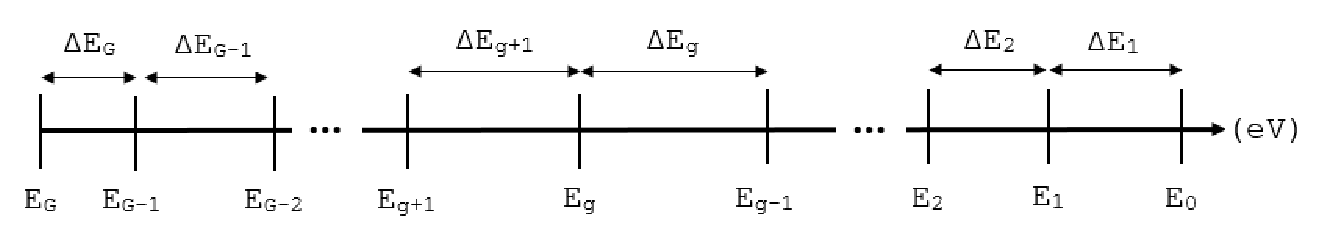
\includegraphics[width=1.00\textwidth]{figures/sec_Sn/MG_Energy_Bands.eps}
\caption{Interval structure of the multigroup methodology.}
\label{fig::Sn_MG_energy_bands}
\end{figure}

For the remainder of this energy discretization procedure, we will utilize the steady-state form of the transport equation in Eq. (\ref{eq::Sn_transport_eq_op_SS}). The time-dependent and eigenvalue forms are analagous and would be derived identically. Taking the energy interval for group $g$ as defined in Eq. (\ref{eq::Sn_MG_energy_interval}), the energy-integrated angular flux of group $g$ is

\begin{equation}
\label{eq::Sn_MG_ang_flux_g}
\Psi_g (\vec{r}, \vec{\Omega}) = \int_{E_g}^{E_{g-1}} \, \Psi (\vec{r}, E, \vec{\Omega}) \, dE .
\end{equation}

\noindent We can then use the energy-integrated angular flux to form the following coupled, $(g=1,...,G)$, discrete equations (we have dropped the spatial parameter and some of the angular parameters for further clarity):

\begin{equation}
\label{eq::Sn_MG_trans_eq}
\left(  \vec{\Omega} \cdot \vec{\nabla} + \sigma_{t,g}  \right) \Psi_g =  \sum_{g'=1}^{G} \left[ \frac{\chi_g}{4 \pi} \nu \sigma_{f,g'} \int_{4 \pi} \Psi_{g'} (\vec{\Omega}') \, d\Omega' + \int_{4 \pi} \sigma_{s}^{g' \rightarrow g} (\vec{\Omega}' , \vec{\Omega} ) \Psi_{g'} (\vec{\Omega}')  \, d\Omega'  \right] + Q_g
\end{equation}

\noindent where

\begin{equation}
\label{eq::Sn_MG_exact_condensed_terms}
\begin{aligned}
\sigma_{t,g} (\vec{r},\vec{\Omega}) & \equiv \frac{\int_{E_{g}}^{E_{g-1}} \sigma_{t} (\vec{r},\vec{\Omega},E) \Psi (\vec{r},\vec{\Omega}, E) \, dE}{\int_{E_{g}}^{E_{g-1}} \int_{4 \pi} \Psi (\vec{r},\vec{\Omega}, E) \, dE}\\
\nu\sigma_{f,g} (\vec{r}) & \equiv \frac{\int_{E_{g}}^{E_{g-1}} \nu\sigma_{f} (\vec{r},E)  \int_{4 \pi} \Psi (\vec{r},\vec{\Omega}, E) \, dE d\Omega}{\int_{E_{g}}^{E_{g-1}} \int_{4 \pi} \Psi (\vec{r},\vec{\Omega}, E) \, dE d\Omega} \\
\chi_g & \equiv \int_{E_{g}}^{E_{g-1}} \chi  (\vec{r},E) \, dE \\
\sigma_{s}^{g' \rightarrow g} (\vec{r},\vec{\Omega}' , \vec{\Omega} ) & \equiv \frac{\int_{E_{g'}}^{E_{g'-1}} \left[ \int_{E_{g}}^{E_{g-1}} \sigma_s (\vec{r},E' \rightarrow E,\vec{\Omega}' , \vec{\Omega} ) \, dE \right] \Psi (\vec{r},\vec{\Omega}', E') \, dE' }{\int_{E_{g}}^{E_{g-1}}  \Psi (\vec{r},\vec{\Omega}, E) \, dE} \\
Q_g (\vec{r}, \vec{\Omega}) & \equiv \int_{E_{g}}^{E_{g-1}} Q (\vec{r}, \vec{\Omega}, E) \, dE
\end{aligned}
\end{equation}

The above equations are mathematically exact to those presented in Eqs. (\ref{eq::Sn_transport_eq_full} - \ref{eq::Sn_transport_eq_op_SS}) and we have made no approximations at this time. However, this requires full knowledge of the energy distribution of the angular flux solution at all positions in our problem domain since we weight the multigroup cross sections with this solution. This is obviously impossible since the energy distibution is part of the solution space we are trying to solve for. Instead, we now define the process to make the multigroup discretization an effective approximation method.

We first define an approximate angular flux distribution for a region $s$:

\begin{equation}
\label{eq::Sn_MG_flux_approx}
\Psi (\vec{r},\vec{\Omega}, E) =  \hat{\Psi} (\vec{r},\vec{\Omega}) f_{s} (E) ,
\end{equation}

\noindent which is a factorization of the angular flux solution into a region-dependent energy function, $f_s (E)$, and a spatially/angularly dependent function, $\hat{\Psi} (\vec{r},\vec{\Omega})$. With this approximation, we can redefine the energy-collapsed cross sections of Eq. (\ref{eq::Sn_MG_exact_condensed_terms}):

\begin{equation}
\label{eq::MG_approx_condensed_terms}
\begin{aligned}
\sigma_{t,g} (\vec{r},\vec{\Omega}) & \equiv \frac{\int_{E_{g}}^{E_{g-1}} \sigma_{t} (\vec{r},\vec{\Omega},E) f_{s} (E) \, dE}{\int_{E_{g}}^{E_{g-1}} f_{s} (E) \, dE} ,\\
\nu\sigma_{f,g} (\vec{r}) & \equiv \frac{\int_{E_{g}}^{E_{g-1}} \nu\sigma_{f} (\vec{r},E)  f_{s} (E) \, dE }{\int_{E_{g}}^{E_{g-1}} f_{s} (E) \, dE}, \\
\sigma_{s}^{g' \rightarrow g} (\vec{r},\vec{\Omega}' , \vec{\Omega} ) & \equiv \frac{\int_{E_{g'}}^{E_{g'-1}} \left[ \int_{E_{g}}^{E_{g-1}} \sigma_s (\vec{r},E' \rightarrow E,\vec{\Omega}' , \vec{\Omega} ) \, dE \right] f_{s} (E')\, dE' }{\int_{E_{g}}^{E_{g-1}}  f_{s} (E) \, dE} .
\end{aligned}
\end{equation}

\noindent It is noted that we do not need to redefine the fission spectrum or the distributed external sources since they are not weighted with the angular flux solution. With this energy factorization, we would expect, in general, that the approximation error will tend to zero as the number of discrete energy groups increases (thereby making the energy bins thinner). This is especially true if the group structure is chosen with many more bins in energy regions with large variations in the energy solution. For certain problems, the region-dependent energy function is well understood ({\em i.e.} almost exactly known). This means, that for these problems, we can achieve reasonable solution accuracy with only a few groups where the energy bins of the multigroup discretization are well chosen. A good example of these kinds of problems are thermal-spectrum nuclear reactors which have historically achieved reasonable solutions with as few as 4-10 energy groups.

%%%%%%%%%%%%%%%%%%%%%%%%%%%%%%%%%%%%%%%%%%%%%%%%%%%
%%%   Section - Angle Discretization
\section{Angular Discretization}
\label{sec::Sn_Angle}

Now that we have provided the discretization of the energy variable, we next focus on the discretization of the transport problem in angle. We will do this in two stages: 1) expand the angular flux in the scattering source and the distributed external source in spherical harmonics and 2) collocate the angular flux at the interpolation points of the trial space. We will perform these discretization procedures by taking the stready-state equation presented in Eq. (\ref{eq::Sn_transport_eq_op_SS}), dropping the fission term and spatial parameterization, and using only 1 energy group:

\begin{equation}
\label{eq::Sn_Angle_simple_trans_eq}
\vec{\Omega} \cdot \vec{\nabla} \Psi (\vec{\Omega}) + \sigma_t \Psi (\vec{\Omega}) = \int_{4 \pi}  d\Omega' \, \sigma_s ( \vec{\Omega}' \cdot \vec{\Omega}) \Psi (\vec{\Omega}') + Q  (\vec{\Omega}) .
\end{equation}

We first expand the angular flux and the scattering cross section in spherical harmonics,

\begin{equation}
\label{eq::Sn_Angle_moments}
\begin{aligned}
	\Phi_{p,n} &\equiv \int_{4 \pi} d\Omega \, \Psi(\vec{\Omega}) \, Y_{p,n} (\vec{\Omega}), \\
	\sigma_{s,p} &\equiv  \int_{-1}^{1} \, d \mu \, \sigma_s ( \mu) P_p (\mu)  ,
\end{aligned}
\end{equation}

\noindent where we have used the following relationships:

\begin{equation}
\label{eq::Sn_Angle_other_terms}
\begin{aligned}
	\mu &\equiv \vec{\Omega}' \cdot \vec{\Omega}, \\
	\sigma_s ( \vec{\Omega}' \cdot \vec{\Omega}) &\equiv  \frac{1}{2 \pi} \sigma_s ( \mu ) ,\\
	P_p ( \vec{\Omega}' \cdot \vec{\Omega}) &\equiv  \frac{1}{2 \pi} P_p (\mu).
\end{aligned}
\end{equation}

\begin{table}[hbt]
\centering
\caption{2D angle mapping from the first quadrant into the other 3 quadrants.}
\begin{tabular}{|c|cc|}
	\hline
	Quadrant & $\mu$ & $\eta$ \\
	\hline
	1 & $\mu_1=\mu_1$ & $\eta_1=\eta_1$ \\
	\hline
	2 & $\mu_2=-\mu_1$ & $\eta_2=\eta_1$ \\
	\hline
	3 & $\mu_3=-\mu_1$ & $\eta_3=-\eta_1$ \\
	\hline
	4 & $\mu_4=\mu_1$ & $\eta_4=-\eta_1$ \\
	\hline
\end{tabular}
\label{tab::Sn_2D_octant_mapping}
\end{table}

\begin{table}[hbt]
\centering
\caption{3D angle mapping from the first octant into the other 7 octants.}
\begin{tabular}{|c|ccc|}
	\hline
	Quadrant & $\mu$ & $\eta$ & $\xi $ \\
	\hline
	1 & $\mu_1=\mu_1$ & $\eta_1=\eta_1$ & $\xi_1=\xi_1$ \\
	\hline
	2 & $\mu_2=-\mu_1$ & $\eta_2=\eta_1$ & $\xi_2=\xi_1$ \\
	\hline
	3 & $\mu_3=-\mu_1$ & $\eta_3=-\eta_1$ & $\xi_3=\xi_1$ \\
	\hline
	4 & $\mu_4=\mu_1$ & $\eta_4=-\eta_1$ & $\xi_4=\xi_1$ \\
	\hline
	5 & $\mu_5=\mu_1$ & $\eta_5=\eta_1$ & $\xi_5=-\xi_1$ \\
	\hline
	6 & $\mu_6=-\mu_1$ & $\eta_6=\eta_1$ & $\xi_6=-\xi_1$ \\
	\hline
	7 & $\mu_7=-\mu_1$ & $\eta_7=-\eta_1$ & $\xi_7=-\xi_1$ \\
	\hline
	8 & $\mu_8=\mu_1$ & $\eta_8=-\eta_1$ & $\xi_8=-\xi_1$ \\
	\hline
\end{tabular}
\label{tab::Sn_3D_octant_mapping}
\end{table}

We conclude our discussion of angular discretizations by presenting two common angular quadrature sets that will be employed in this dissertation work. Section \ref{sec::Sn_Angle_LS} presents the Level Symmetric (LS) quadrature set and Section \ref{sec::Sn_Angle_PGLC} presents the Product Gauss-Legendre-Chebyshev (PGLC) quadrature set.

%%%%%%%%%%%%%%%%%%%%%%%%%%%%%%%%%%%%%%%%%%%%%%%%%%%
%%%   SubSection - Level-Symmetric
\subsection{Level-Symmetric Quadrature Set}
\label{sec::Sn_Angle_LS}

The first quadrature set we present is the common Level Symmetric set.

\begin{figure}
\centering
	\begin{subfigure}[b]{0.48\textwidth}
		\centering
		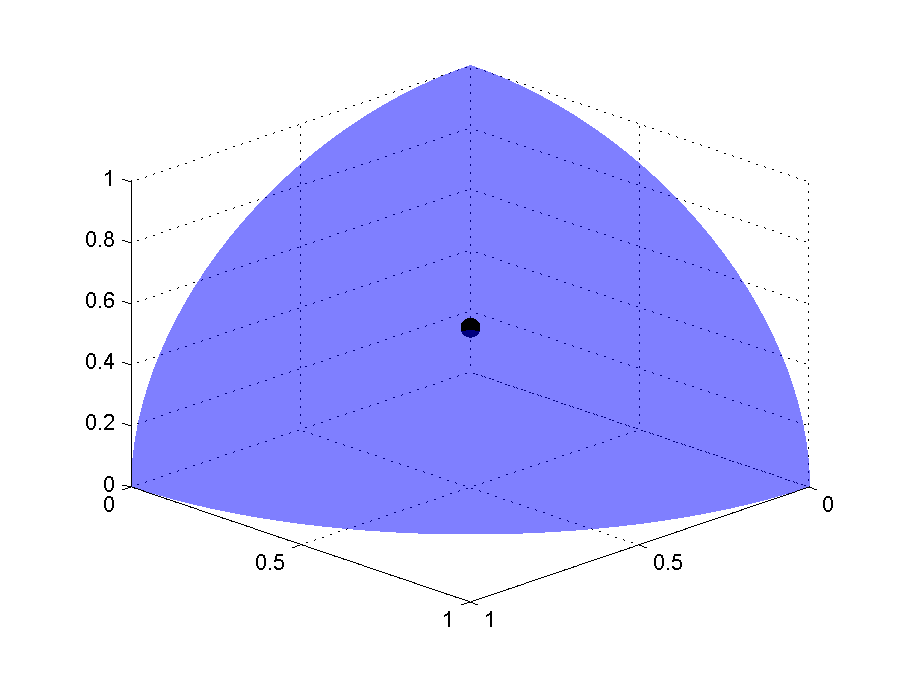
\includegraphics[width=0.92\textwidth]{figures/sec_Sn/LS2.eps}
		\caption{}
	\end{subfigure}
	\hfill
	\begin{subfigure}[b]{0.48\textwidth}
		\centering
		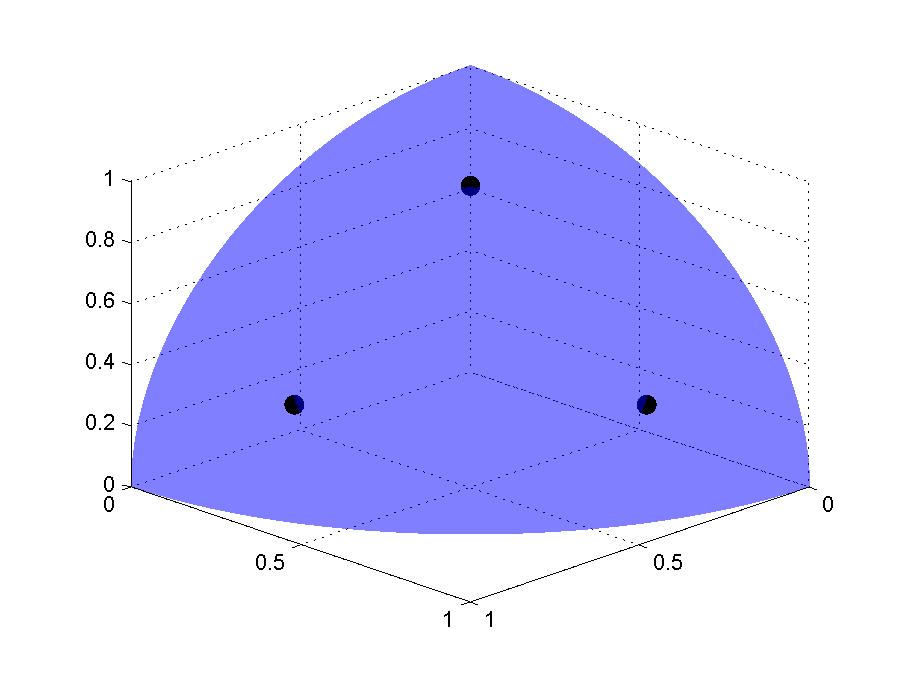
\includegraphics[width=0.92\textwidth]{figures/sec_Sn/LS4.eps}
		\caption{}
	\end{subfigure}
	\vfill
	\begin{subfigure}[b]{0.48\textwidth}
		\centering
		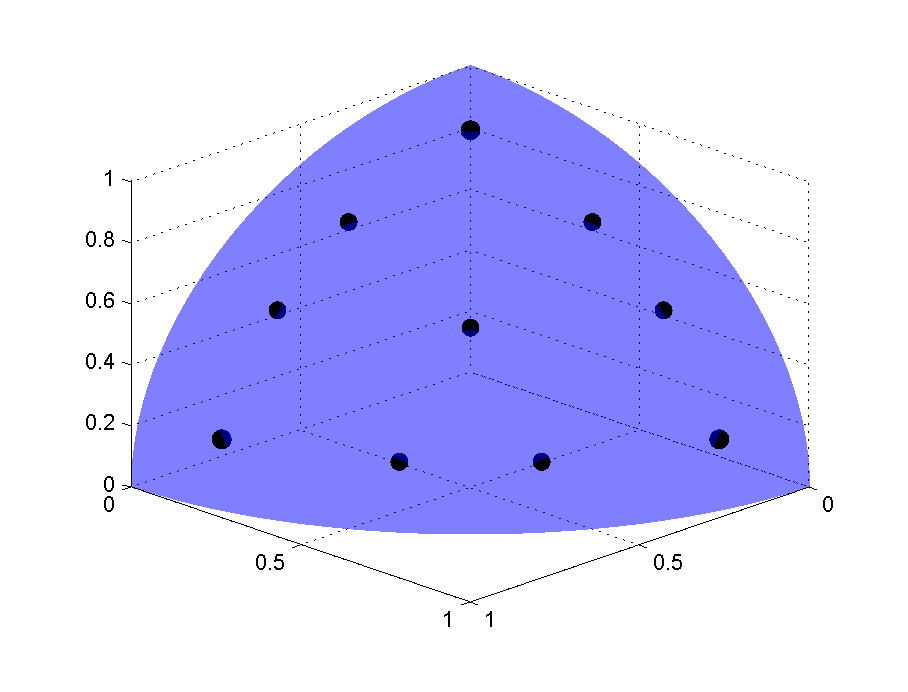
\includegraphics[width=0.92\textwidth]{figures/sec_Sn/LS8.eps}
		\caption{}
	\end{subfigure}
	\hfill
	\begin{subfigure}[b]{0.48\textwidth}
		\centering
		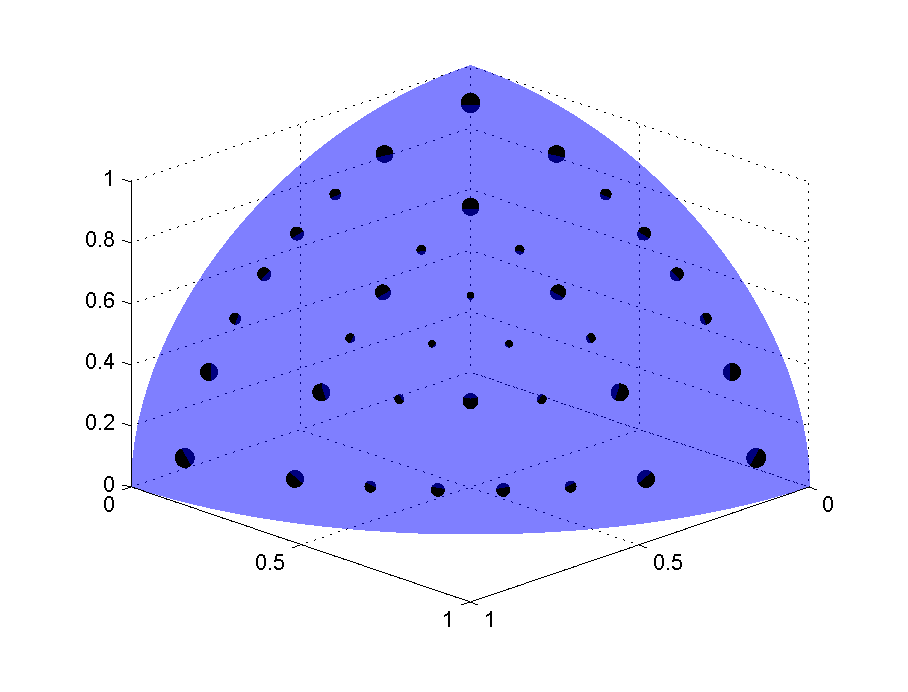
\includegraphics[width=0.92\textwidth]{figures/sec_Sn/LS16.eps}
		\caption{}
	\end{subfigure}
\caption[Level-Symmetric angular quadrature set]{Level-Symmetric angular quadrature set of order (a) 2, (b) 4, (c) 8, and (d) 16.}
\label{fig::Sn_Angle_LS_Quads}
\end{figure}

%%%%%%%%%%%%%%%%%%%%%%%%%%%%%%%%%%%%%%%%%%%%%%%%%%%
%%%   SubSection - PGLC
\subsection{Product Gauss-Legendre-Chebyshev Quadrature Set}
\label{sec::Sn_Angle_PGLC}

The second angular quadrature set we will present is a Product Gauss-Legendre-Chebyshev (PGLC) set. It is formed by the product-wise multiplication of a Gauss-Chebyshev quadrature in the azimuthal direction and a Gauss-Legendre quadrature in the polar direction. It has the following key differences from the Level Symmetric set:

\begin{itemize}
	\item Does not have $90^o$ rotational invariance within the primary octant; still maintains octant-to-octant symmetry however;
	\item Has more control over the placement of the anglular directions within the primary octant;
	\item Quadrature weights are aligned with the polar level;
	\item Has strictly positive weights for all polar and azimuthal combinations.
\end{itemize}

From the listed differences, we can already discern some clear advantages and disadvantages from a fully-symmetric quadrature set like LS. If a high number of angles are required for a problem, then negative weights do not arise. This is beneficial for transport problems with significant discontinuities. Also, the quadrature directions can be preferentially distributed in the primary octant if required for a particular problem. For example, if the transport solution is smoothly varying in the polar direction and not in the azimuthal direction, then we can specify a larger number of quadrature points in the azimuthal direction, with much fewer points in the polar direction. However, this also highlights the fact that the quadrature weights are aligned with the polar level, which can lead to less accurate moment integrations for certain transport problems. 

For this dissertation, we will use the following notation to define the product nature of the PGLC quadrature points: $S_{a}^{p}$. Here, $a$ and $p$ correspond to the number of azimuthal and polar directions in the primary octant, respectively. We demonstrate this definition in Figure \ref{fig::Sn_Angle_PGLC_Quads} with several combinations of azimuthal and polar directions. Again, the size of the direction marker corresponds to the relative weight of quadrature point. One can clearly see that the weights vary on the polar levels and all azimuthal weights on a given polar level are constant.

\begin{figure}
\centering
	\begin{subfigure}[b]{0.48\textwidth}
		\centering
		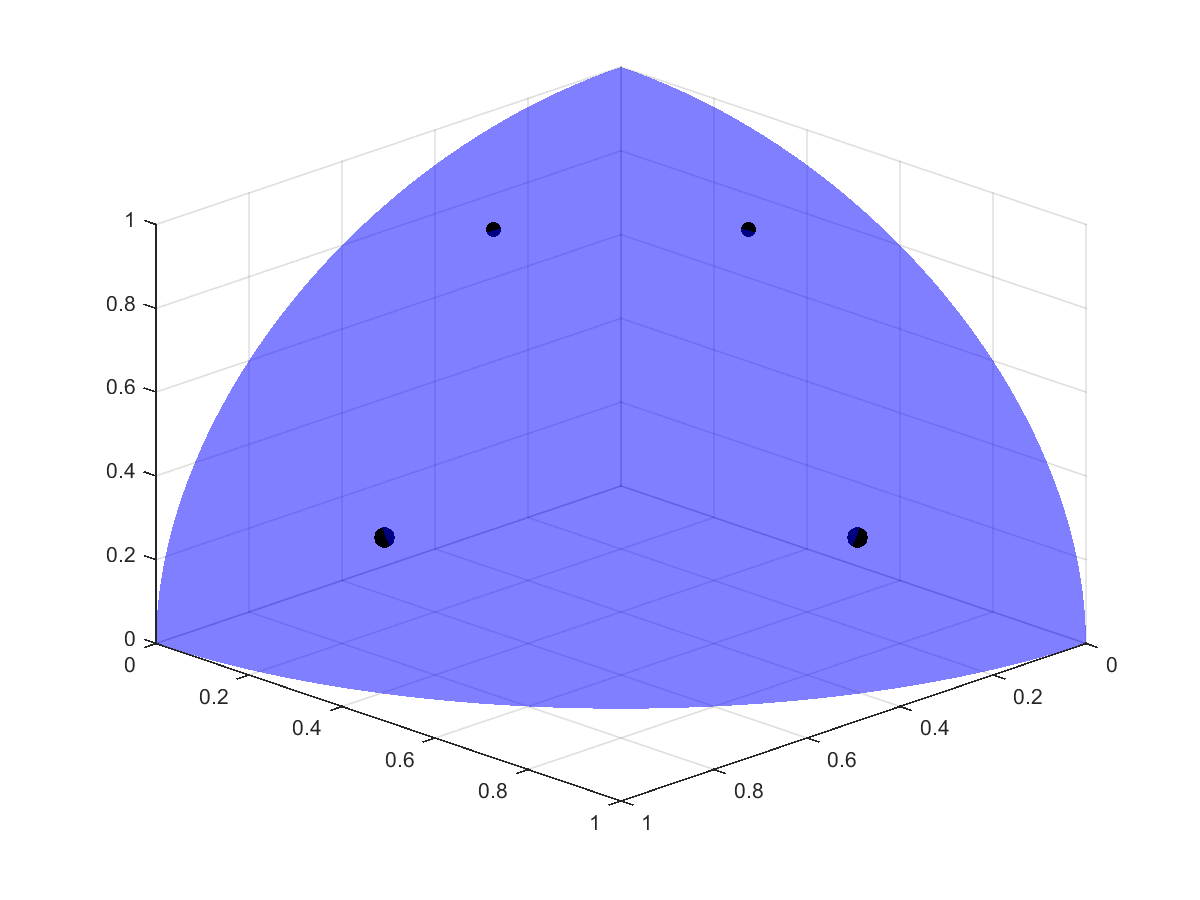
\includegraphics[width=0.92\textwidth]{figures/sec_Sn/PGLC2_2.png}
		\caption{}
	\end{subfigure}
	\hfill
	\begin{subfigure}[b]{0.48\textwidth}
		\centering
		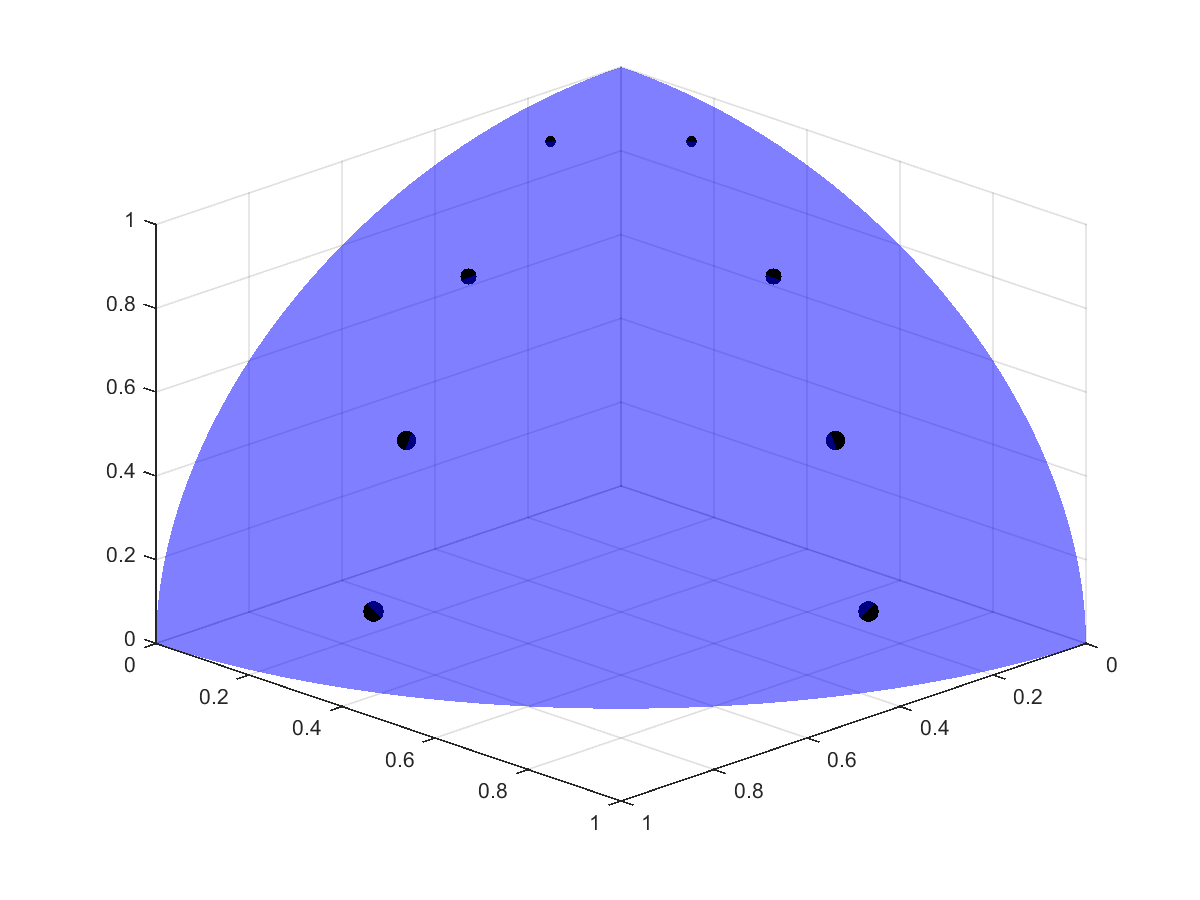
\includegraphics[width=0.92\textwidth]{figures/sec_Sn/PGLC2_4.png}
		\caption{}
	\end{subfigure}
	\vfill
	\begin{subfigure}[b]{0.48\textwidth}
		\centering
		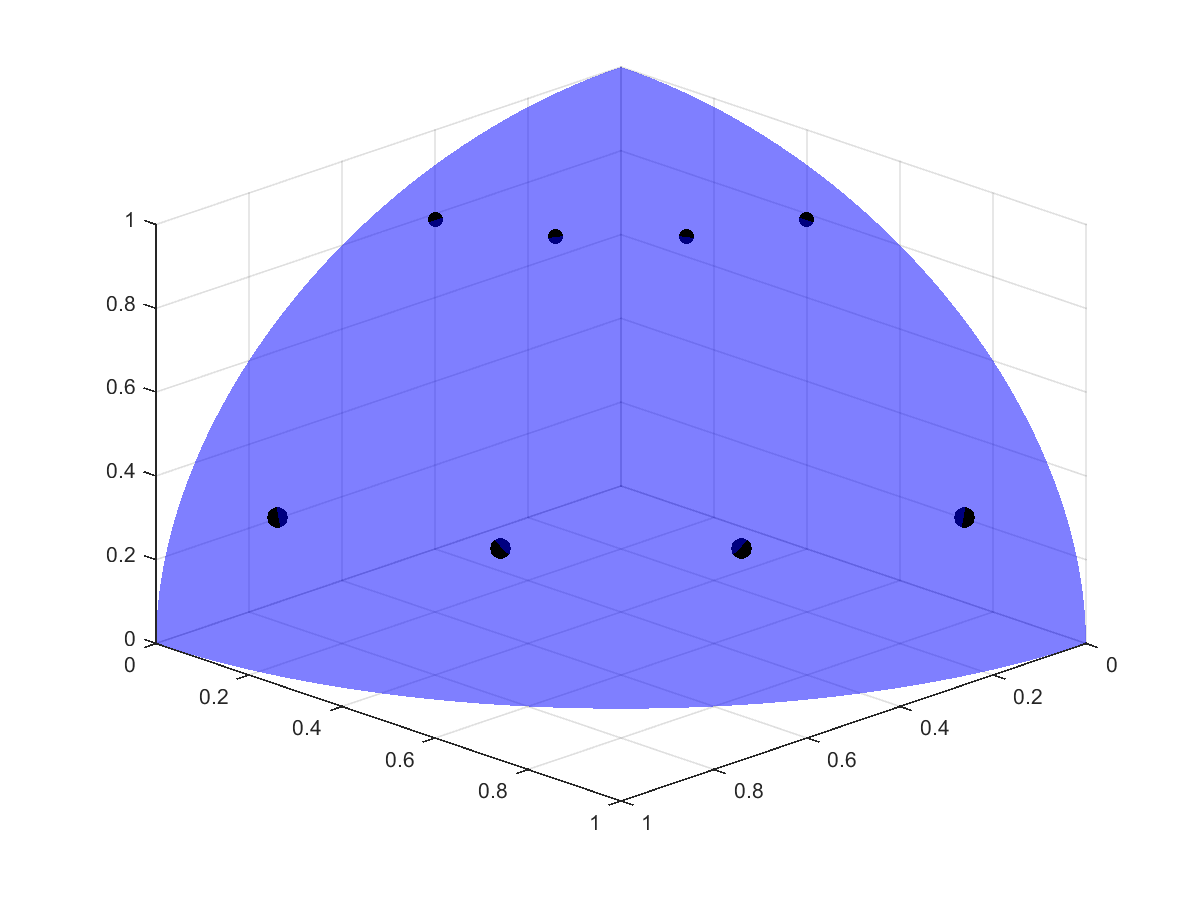
\includegraphics[width=0.92\textwidth]{figures/sec_Sn/PGLC4_2.png}
		\caption{}
	\end{subfigure}
	\hfill
	\begin{subfigure}[b]{0.48\textwidth}
		\centering
		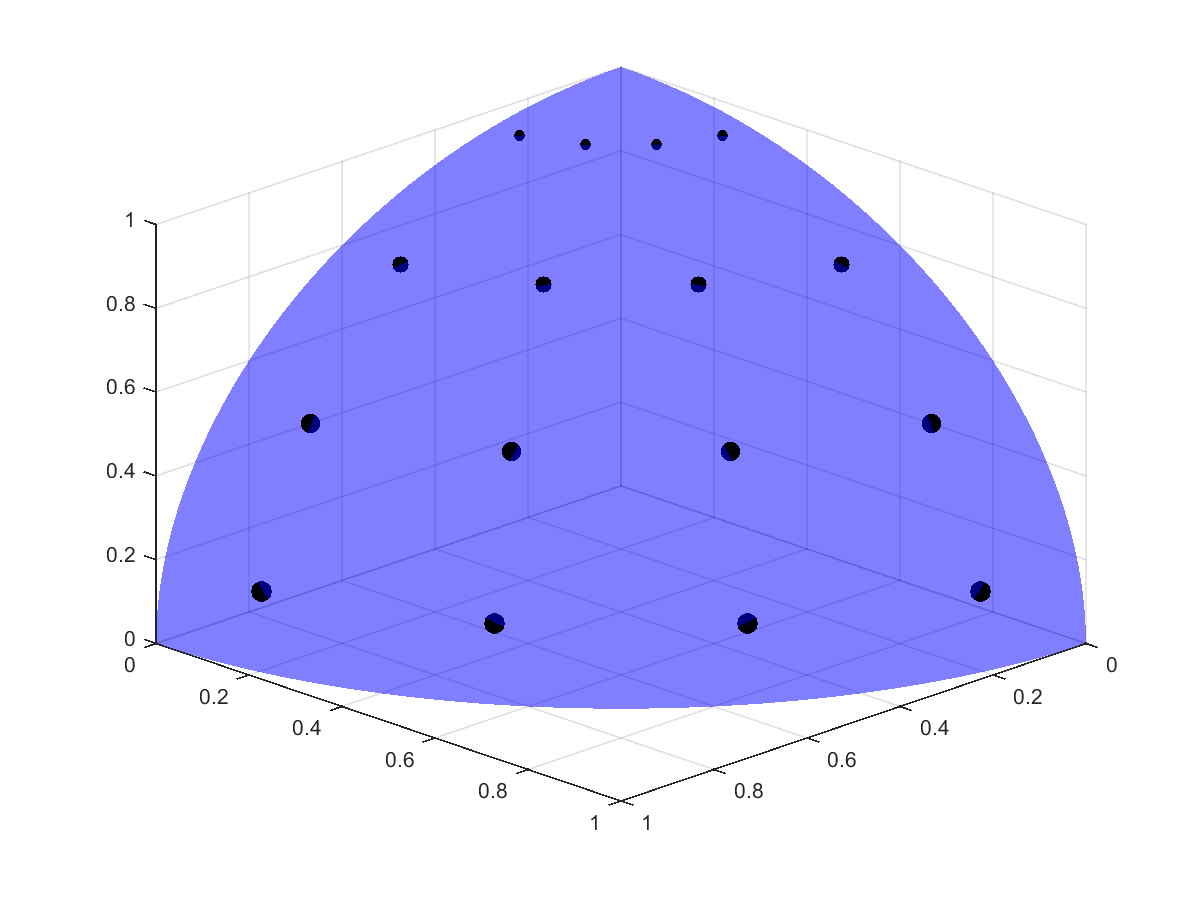
\includegraphics[width=0.92\textwidth]{figures/sec_Sn/PGLC4_4.png}
		\caption{}
	\end{subfigure}
	\vfill
	\begin{subfigure}[b]{0.48\textwidth}
		\centering
		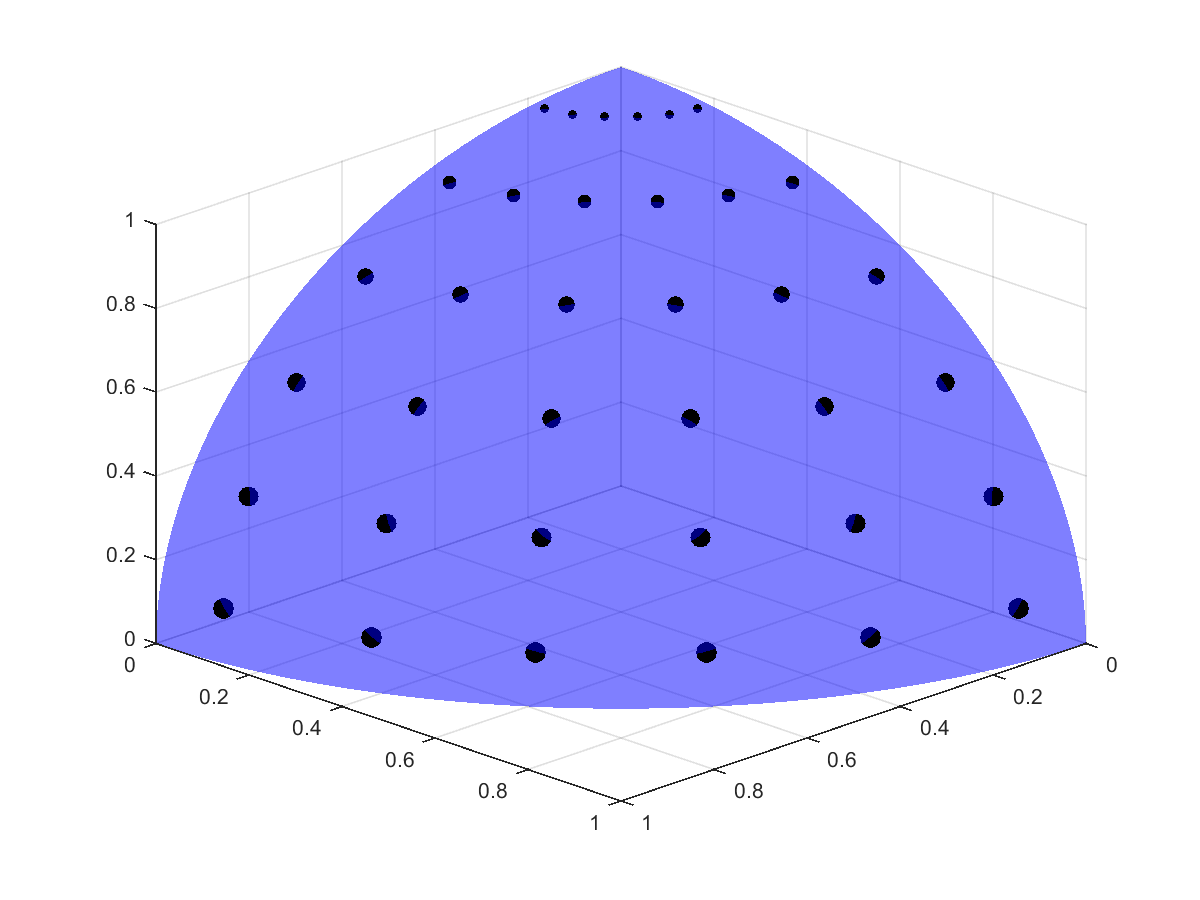
\includegraphics[width=0.92\textwidth]{figures/sec_Sn/PGLC6_6.png}
		\caption{}
	\end{subfigure}
	\hfill
	\begin{subfigure}[b]{0.48\textwidth}
		\centering
		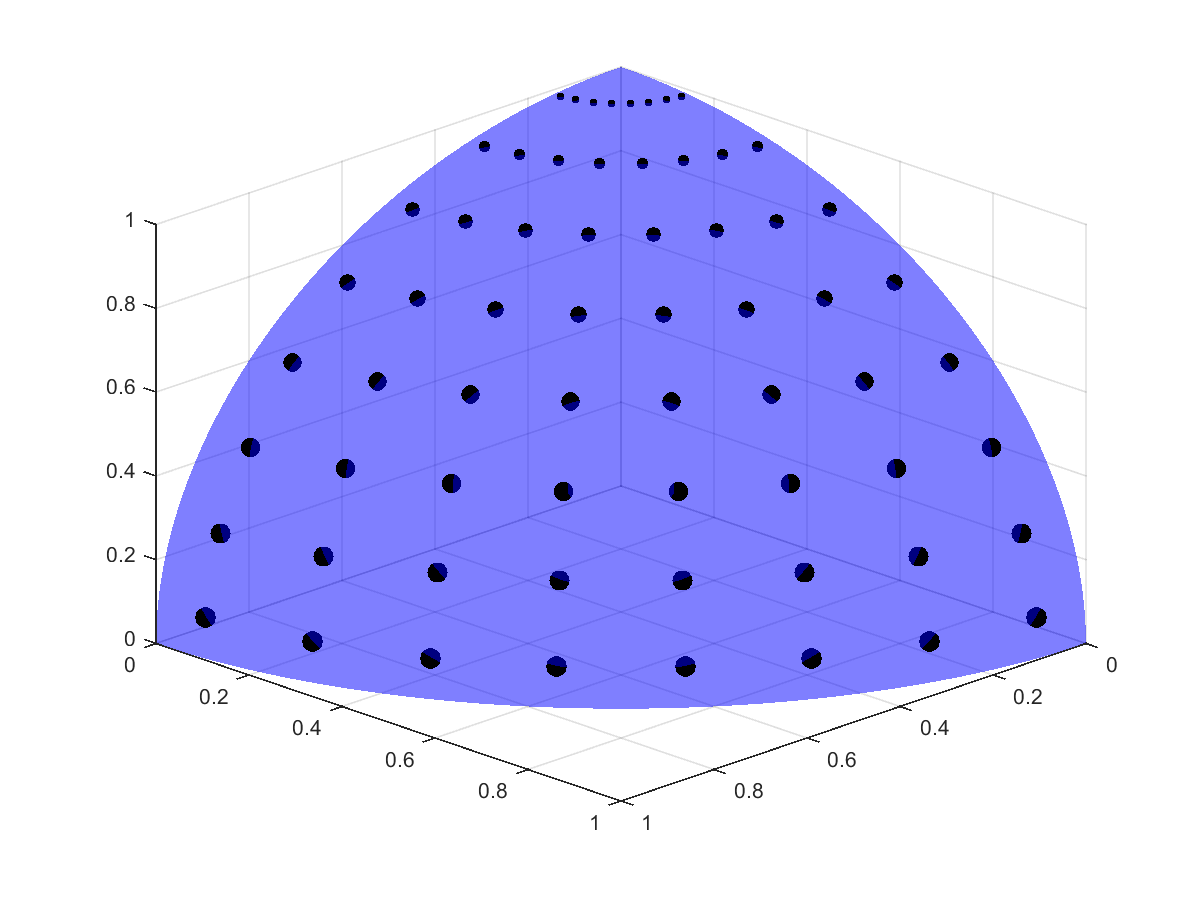
\includegraphics[width=0.92\textwidth]{figures/sec_Sn/PGLC8_8.png}
		\caption{}
	\end{subfigure}
\caption[Product Gauss-Legendre-Chebyshev angular quadrature set]{Product Gauss-Legendre-Chebyshev angular quadrature set with orders: (a) S$_2^2$, (b) S$_2^4$, (c) S$_4^2$, (d) S$_4^4$, (e) S$_6^6$, and (f) S$_8^8$.}
\label{fig::Sn_Angle_PGLC_Quads}
\end{figure}

%%%%%%%%%%%%%%%%%%%%%%%%%%%%%%%%%%%%%%%%%%%%%%%%%%%
%%%   Section - Boundary Conditions
\section{Boundary Conditions}
\label{sec::Sn_BC}

Using the energy and angular discretizations presented in Sections \ref{sec::Sn_MG} and \ref{sec::Sn_Angle}, respectively, we write the standard, steady-state, multigroup $S_N$ transport equation for one angular direction, $m$, and one energy group, $g$:

\begin{equation}
\label{eq::Sn_mg_sn_trans_eq}
\begin{aligned}
	 \left( \vec{\Omega}_m \cdot \vec{\nabla}  + \sigma_{t,g}  \right)  \Psi_{m,g}= \sum_{g'=1}^{G} \sum_{p=0}^{N_P} \frac{2p + 1}{4 \pi} \sigma_{s,p}^{g' \rightarrow g}   \sum_{n=-p}^{p}  \Phi_{p,n,g'}  Y_{p,n} (  \vec{\Omega}_m )  \\
	+ \frac{\chi_g}{4 \pi} \sum_{g'=1}^{G} \nu \sigma_{f,g'} \Phi_{g'}   + Q_{m,g}
\end{aligned} , 
\end{equation}

\noindent where we have dropped the spatial parameter for clarity and is beholden to the following general, discretized boundary condition:

\begin{equation}
\label{eq::Sn_mg_sn_trans_eq_bc}
\Psi_{m,g} (\vec{r}) = \Psi^{inc}_{m,g} (\vec{r}) + \sum_{g'=1}^{G} \sum_{\vec{\Omega}_{m'} \cdot \vec{n} > 0} \gamma_{g' \rightarrow g}^{m' \rightarrow m} (\vec{r})  \Psi_{m',g'} (\vec{r})  .
\end{equation}

\noindent These $(M \text{x} G)$ number of discrete, tightly-coupled equations are currently defined as continuous in space.

For this dissertation work, we will consider only one type of boundary conditions: Dirichlet-type boundaries (also called {\em first-type boundary condition} in some physics and mathematical communities). In particular we will only utilize incoming-incident and reflecting boundary conditions which correspond to $\vec{r} \in \partial \mathcal{D}^d$ and $\vec{r} \in \partial \mathcal{D}^r$, respectively. The full domain boundary is then the union: $\partial \mathcal{D} = \partial \mathcal{D}^d \cup \partial \mathcal{D}^r$. This leads to the boundary condition being succinctly written for one angular direction, $m$, and one energy group, $g$ as

\begin{equation}
\label{eq::Sn_simple_BC}
\Psi_{m,g} (\vec{r}) = \begin{cases}
	\Psi^{inc}_{m,g} (\vec{r}) , & \vec{r} \in \partial \mathcal{D}^d \\
	\Psi_{m',g} (\vec{r}) , & \vec{r} \in \partial \mathcal{D}^r
\end{cases}
\end{equation}

\noindent where the reflecting angle is $\vec{\Omega}_{m'} = \vec{\Omega}_{m} - 2 \left(  \vec{\Omega}_{m} \cdot \vec{n} \right) \vec{n}$ and $\vec{n}$ is oriented outward from the domain. To properly utilize the reflecting boundary condition that we have proposed, the angular quadrature set defined in Section \ref{sec::Sn_Angle} needs the following properties.

\begin{enumerate}
 	\item The reflected directions, $\vec{\Omega}_{m'}$, are also in the quadrature set for all $\vec{r} \in \partial \mathcal{D}^r$.
	\item The weights of the incident, $w_m$, and reflected, $w_{m'}$, angles must be equal.
\end{enumerate} 

\noindent For problems where the reflecting boundaries align with the $x,y,z$ axes, this will not be an issue with standard quadrature sets ({\em e.g.} level-symmetric or Gauss-Legendre-Chebyshev). However, if the reflecting boundaries do not align in this manner, then additional care must be employed in calculating appropriate angular quadrature sets.

%%%%%%%%%%%%%%%%%%%%%%%%%%%%%%%%%%%%%%%%%%%%%%%%%%%
%%%   Section - Spatial Discretization
\section{Spatial Discretization}
\label{sec::Sn_Spatial}

For the spatial discretization of the problem domain, we simplify Eq. (\ref{eq::Sn_mg_sn_trans_eq}) into a single energy group and drop the fission term (it can be lumped into the 0th order external source term and will act similarly to the total interaction term)

\begin{equation}
\label{eq::Sn_trans_eq_simple_no_energy_groups}
\vec{\Omega}_m \cdot \vec{\nabla} \Psi_{m}  + \sigma_{t}   \Psi_{m}=  \sum_{p=0}^{N_P} \frac{2p + 1}{4 \pi}    \sum_{n=-p}^{p}  Y_{p,n} (  \vec{\Omega}_m ) \left[ \sigma_{s,p}  \Phi_{p,n,}  + Q_{p,n} \right]
\end{equation}

\noindent to form $M$ ($m=1,...,M$) angularly discrete equations. We then lay down an unstructured mesh, $\mathbb{T}_h \in \mathbb{R}^{d}$, over the spatial domain, where $d$ is the dimensionality of the problem ($d=1,2,3$). This mesh consists of non-overlapping spatial elements to form a complete union over the entire spatial domain: $\mathcal{D} = \bigcup_{K \in \mathbb{T}_h} K$. To form the DGFEM set of equations \cite{ern2013theory,wareing2001discontinuous}, we consider a spatial cell $K \in \mathbb{R}^d$ which has $N_V^K$ vertices and $N_f^K$ faces. Each face of cell $K$ resides in dimension $\mathbb{R}^{d-1}$ and is formed by a connection of a subset of vertices. For a 1D problem, each face is a single point. For a 2D problem, each face is a line segment connecting two distinct points. For a 3D problem, each face is a $\mathbb{R}^2$ closed polygon (not necessarily coplanar) which may or not be convex. An example of this interconnection between elements is given for a $\mathbb{R}^2$ problem in Figure \ref{fig::Sn_two_ref_cells} between our cell of interest, $K$, and another cell, $K'$, separated by the face $f$. We have chosen the normal direction of the face to have orientation from cell $K$ to cell $K'$ while we form the DGFEM equations for cell $K$. This means that if we were instead analyzing cell $K'$, then the face $f$ normal, $\vec{n}' $, would be opposite ({\em i.e.} $\vec{n}' = -\vec{n}$).

\begin{figure}
\centering
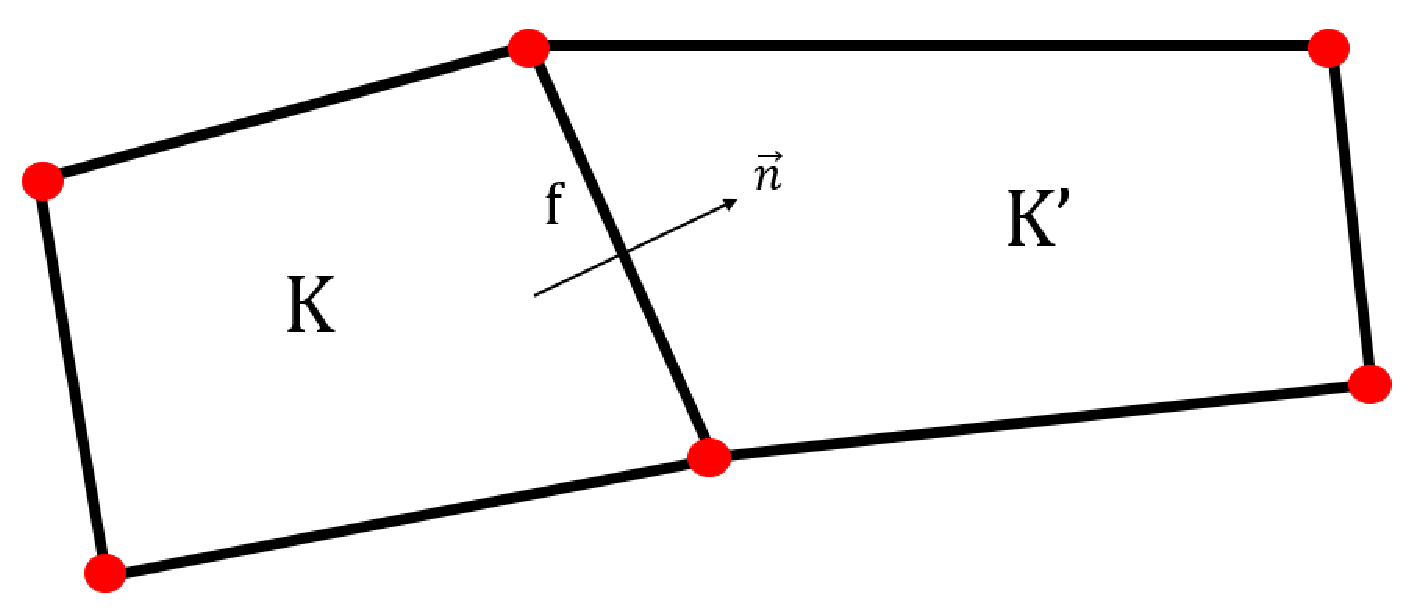
\includegraphics[width=0.7\textwidth]{figures/sec_Sn/two_cells_Rev1.eps}
\caption[Two cells of the spatial discretization]{Two cells of the spatial discretization with the connecting face, $f$, with normal direction, $\vec{n}$, oriented from cell $K$ to cell $K'$.}
\label{fig::Sn_two_ref_cells}
\end{figure}

Next, we left-multiply Eq. (\ref{eq::Sn_trans_eq_simple_no_energy_groups}) by an appropriate test function $b_m$, integrate over cell $K$, and apply Gauss' Divergence Theorem to the streaming term to obtain the Galerkin weighted-residual for cell $K$ for an angular direction $\vec{\Omega}_m$:

\begin{equation}
\label{eq::Sn_DGFEM_trans_eq_cellK}
\begin{aligned}
- \left( \vec{\Omega}_m \cdot  \vec{\nabla} b_m, \Psi_{m} \right)_{K} + \sum_{f=1}^{N_f^K} \Big< ( \vec{\Omega}_m \cdot \vec{n} ) \, b_m, \tilde{\Psi}_m  \Big>_{f}  + \Big(  \sigma_{t} b_m ,   \Psi_{m} \Big)_{K} \\
= \sum_{p=0}^{N_P} \sum_{n=-p}^{p} \frac{2p + 1}{4 \pi}  Y_{p,n} (  \vec{\Omega}_m ) \left[ \Big( \sigma_{s,p} \, b_m,  \Phi_{p,n,} \Big)_{K}  + \left(  b_m ,   Q_{p,n} \right)_{K} \right]
\end{aligned} .
\end{equation}

\noindent The cell boundary fluxes, $\tilde{\Psi}_m$, will depend on the cell boundary type and will be defined shortly. The cell boundary $\partial \mathcal{D}_K = \bigcup_{ f \in N_f^K} f$ is the closed set of the $N_f^K$ faces of the geometric cell. The inner products:

\begin{equation}
\label{eq::Sn_spatial_inner_products_cell}
 \Big( f, g \Big)_K \equiv \int_K f \, g \, d r
\end{equation} 

\noindent and

\begin{equation}
\label{eq::Sn_spatial_inner_products_face}
 \Big< f, g \Big>_f \equiv \int_f f \, g \, d s
\end{equation}

\noindent correspond to integrations over the cell and faces, respectively, where $dr \in \mathbb{R}^d$ is within the cell and $ds \in \mathbb{R}^{d-1}$ is along the cell boundary. We note that we will use this notation of the inner product for the remainder of the dissertation unless otherwise stated. We then separate the summation of the cell $K$ boundary integration terms into two different types: outflow boundaries ($\partial K^+ = \{  \vec{r} \in \partial K: \vec{n} (\vec{r}) \cdot \vec{\Omega}_m > 0 \}$) and inflow boundaries ($\partial K^- = \{  \vec{r} \in \partial K: \vec{n} (\vec{r}) \cdot \vec{\Omega}_m < 0 \}$). The inflow boundaries can further be separated into inflow from another cell: $\partial K^- \backslash \partial \mathcal{D} $; inflow from incident flux on the domain boundary: $\partial K^- \cap \partial \mathcal{D}^d $; and reflecting domain boundaries: $\partial K^- \cap \partial \mathcal{D}^r $. At this point, we note that the derivation can comprise an additional step by using Gauss' Divergence Theorem again on the streaming term. This is sometimes performed for radiation transport work so that mass matrix lumping can be performed, but we will not do so here. Therefore, with the cell boundary terminology as proposed, Eq. (\ref{eq::Sn_DGFEM_trans_eq_cellK}) can be written into the following form:

\begin{equation}
\label{eq::Sn_DGFEM_trans_eq_cellK_diff_faces}
\begin{aligned}
- \left( \vec{\Omega}_m \cdot  \vec{\nabla} b_m, \Psi_{m} \right)_{K}   + \Big(  \sigma_{t} b_m ,   \Psi_{m} \Big)_{K}  \\
+  \Big< ( \vec{\Omega}_m \cdot \vec{n} ) \, b_m, \tilde{\Psi}_m  \Big>_{\partial K^+}  + \Big< ( \vec{\Omega}_m \cdot \vec{n} ) \, b_m, \tilde{\Psi}_m  \Big>_{\partial K^- \backslash \partial \mathcal{D}} \\
  + \Big< ( \vec{\Omega}_m \cdot \vec{n} ) \, b_m, \tilde{\Psi}_m  \Big>_{\partial K^- \cap \partial \mathcal{D}^d}  + \Big< ( \vec{\Omega}_m \cdot \vec{n} ) \, b_m, \tilde{\Psi}_m  \Big>_{\partial K^- \cap \partial \mathcal{D}^r}  \\
= \sum_{p=0}^{N_P} \sum_{n=-p}^{p} \frac{2p + 1}{4 \pi}  Y_{p,n} (  \vec{\Omega}_m ) \left[ \Big( \sigma_{s,p} \, b_m,  \Phi_{p,n,} \Big)_{K}  + \left(  b_m ,   Q_{p,n} \right)_{K} \right]
\end{aligned} .
\end{equation}

We can now deal with the boundary fluxes, $\tilde{\Psi}_m$, by enforcing the ubiquitously-used {\em upwind scheme}. In simple nomenclature, the upwind scheme corresponds to using the angular flux values within the cell for outflow boundaries and angular flux values outside the cell for inflow boundaries. Mathematically, the upwind scheme can succinctly be written as the following for all boundary types,

\begin{equation}
\label{eq::Sn_upwind_cases}
\tilde{\Psi}_m (\vec{r}) = \begin{cases}
\Psi_m^{-} , & \partial K^+ \\
\Psi_m^{+}, & \partial K^- \backslash \partial \mathcal{D} \\
\Psi_m^{inc}, & \partial K^- \cap \partial \mathcal{D}^d \\
\Psi_{m'}^{-}, & \partial K^- \cap \partial \mathcal{D}^r
\end{cases} ,
\end{equation}

\noindent when the following trace is applied to the angular fluxes :

\begin{equation}
\label{eq::Sn_ang_flux_trace}
\Psi_m^{\pm} (\vec{r}) \equiv \lim_{s \rightarrow 0^{\pm}} \Psi_m \Big( \vec{r} + s (\vec{\Omega}_m \cdot \vec{n}) \vec{n} \Big) .
\end{equation}

\noindent This trace has the notation, with $\vec{n}$ pointing outwards from cell $K$, of $\Psi_m^-$ corresponding to fluxes within the cell and $\Psi_m^+$ corresponding to fluxes out of the cell. Now, using the upwind scheme as previously defined, we can write our complete set of DGFEM equations for cell $K$ as

\begin{equation}
\label{eq::Sn_DGFEM_trans_eq_cellK_complete}
\begin{aligned}
-  \Big( \vec{\Omega}_m \cdot  & \vec{\nabla} b_m, \Psi_{m} \Big)_{K}   + \Big(  \sigma_{t} b_m ,   \Psi_{m} \Big)_{K} +  \Big< ( \vec{\Omega}_m \cdot \vec{n} ) \, b_m, {\Psi}_m^{-}  \Big>_{\partial K^+}  \\
  + & \Big< ( \vec{\Omega}_m \cdot \vec{n} ) \, b_m, {\Psi}_m^{+}  \Big>_{\partial K^- \backslash \partial \mathcal{D}}  + \Big< ( \vec{\Omega}_m \cdot \vec{n} ) \, b_m, {\Psi}^{-}_{m'}  \Big>_{\partial K^- \cap \partial \mathcal{D}^r}  \\
= & \sum_{p=0}^{N_P} \sum_{n=-p}^{p} \frac{2p + 1}{4 \pi}  Y_{p,n} (  \vec{\Omega}_m ) \left[ \Big( \sigma_{s,p} \, b_m,  \Phi_{p,n,} \Big)_{K}  + \left(  b_m ,   Q_{p,n} \right)_{K} \right] \\
+ & \Big< ( \vec{\Omega}_m \cdot \vec{n} ) \, b_m, {\Psi}_m^{inc}  \Big>_{\partial K^- \cap \partial \mathcal{D}^d}
\end{aligned} .
\end{equation} 

\noindent We note that fluxes without the trace superscript are all within the cell. By completely defining our mathematical formulation for an arbitrary spatial cell, it is easy to see that the full set of equations to define our discretized solution space for a single angle and energy group comprises of a simple double integration loop. The full set of equations can be formed by looping over all spatial cells, $\mathcal{D} = \bigcup_{K \in \mathbb{T}_h} K$, while further looping over all faces within each cell, $\partial \mathcal{D}_K = \bigcup_{ f \in N_f^K} f$. Section \ref{sec::Sn_Solution} will further detail how all the DGFEM equations are formed along with efficient solution methods. We conclude this section by defining the elementary matrix terms for a given cell as follows.

%%%%%%%%%%%%%%%%%%%%%%%%%%%%%%%%%%%%%%%%%%%%%%%%%%%
%%%   SubSection - Mass
\subsection{Elementary Mass Matrices}
\label{sec::Sn_Spatial_Mass}

In the spatially discretized equations presented in Section \ref{sec::Sn_Spatial}, there are several reaction terms that appear with the form: $\Big( \sigma  b_m , \Psi_m  \Big)_K$ for a given angular direction, $m$, and for a spatial cell, $K$. In FEM analysis these reaction terms are ubiquitously referred to as the mass matrix terms \cite{zeinkiewicz2005finite,akin1982application}. For cell $K$, we define the elementary mass matrix, ${\bf M}$ as

\begin{equation}
\label{eq::Sn_mass_matrix_analytical}
{\bf M}_K =    \int_K {\bf b}_K \, {\bf b}_K^T \, d r ,
\end{equation}

\noindent where ${\bf b}_K$ corresponds to the set of $N_K$ basis functions that have non-zero measure in cell $K$. Depending on the FEM basis functions utilized, the integrals in Eq. (\ref{eq::Sn_mass_matrix_analytical}) can be directly integrated analytically. However, if in general, the basis functions cannot be analytically integrated on an arbitrary set of cell shapes, then a numerical integration scheme becomes necessary. If we define a quadrature set, $\left\{  \vec{x}_q , w_q^{K}  \right\}_{q=1}^{N_q}$, for cell $K$, consisting of $N_q$ points, $\vec{x}_q$, and weights, $w_q^K$, then we can numerically calculate the mass matrix by the following

\begin{equation}
\label{eq::Sn_mass_matrix_numerical}
{\bf M}_K =    \sum_{q = 1}^{N_q} w_{q}^K {\bf b}_K (\vec{x}_q) \, {\bf b}_K^T (\vec{x}_q)  .
\end{equation}

\noindent In this case, it is necessary that the sum of the weights of this quadrature set exactly equal the geometric measure of cell $K$. This means that $\sum_{q = 1}^{N_q} w_{q}^K$ is equal to the cell width in 1 dimension, the cell area in 2 dimensions, and the cell volume in 3 dimensions.

Since ${\bf b}_K$ consists of a column vector for the basis functions and ${\bf b}_K^{T}$ consists of a row vector, then their multiplication will obviously yield a full $(N_K \, \text{x} \, N_K)$ matrix. This matrix is written for completeness of this discussion on the mass matrix:

\begin{equation}
\label{eq::Sn_mass_matrix_array}
{\bf M}_K =   \left[
\begin{array} {ccccc}
	\int_K b_1 \, b_1  & \ldots & \int_K b_1 \, b_j  & \ldots & \int_K b_1 \, b_{N_K} \\
	\vdots  &  & \vdots  &  & \vdots \\
	\int_K b_i \, b_1  & \ldots & \int_K b_i \, b_j  & \ldots & \int_K b_i \, b_{N_K} \\
	\vdots  &  & \vdots  &  & \vdots \\
	\int_K b_{N_K} \, b_1  & \ldots & \int_K b_{N_K} \, b_j  & \ldots & \int_K b_{N_K} \, b_{N_K} \\
\end{array}
\right] ,
\end{equation}

\noindent where an individual matrix entry is of the form:

\begin{equation}
\label{eq::Sn_mass_matrix_entry}
M_{i,j}^K =  \int_K b_i \, b_j .
\end{equation}

%%%%%%%%%%%%%%%%%%%%%%%%%%%%%%%%%%%%%%%%%%%%%%%%%%%
%%%   SubSection - Streaming
\subsection{Elementary Streaming Matrices}
\label{sec::Sn_Spatial_Streaming}

Next, we will consider the streaming term that has the form: $ \Big( \vec{\Omega}_m \cdot \vec{\nabla}  b_m , \Psi_m  \Big)_K$ for a given angular direction, $m$, and for a spatial cell, $K$. $\vec{\nabla} $ is the gradient operator in physical space. It has the form of $\vec{\nabla} = \left[ \frac{d}{dx} \right]$ in 1 dimension, the form of $\vec{\nabla} = \left[ \frac{\partial}{\partial x} , \frac{\partial}{\partial y} \right]$ in 2 dimensions, and the form of $\vec{\nabla} = \left[ \frac{\partial}{\partial x} , \frac{\partial}{\partial y} , \frac{\partial}{\partial z} \right]$ in 3 dimensions. Since for every cell, the streaming term is applied for all $M$ angles in the angular discretization, we define the analytical elementary streaming matrix:

\begin{equation}
\label{eq::Sn_streaming_matrix_analytical}
\vec{{\bf G}}_K =    \int_K \vec{\nabla} {\bf b}_K \, {\bf b}_K^T \, d r ,
\end{equation}

\noindent which has dimensionality $(N_K \text{x} N_K \text{x} d)$. We choose to store the elementary streaming matrix in this form and not store $M$ separate $(N_K \text{x} N_K)$ local matrices corresponding to the application of the dot product ($ \vec{\Omega}_m  \cdot \int_K  \vec{\nabla} {\bf b}_K \, {\bf b}_K^T \, d r$). Instead we simply evaluate the dot product with the appropriate angular direction whenever necessary. This has great benefit when trying to run large transport problems when memory becomes a premium and processor operations are not our limiting bottleneck. 

Just like the elementary mass matrix, we can use the same spatial quadrature set, $\left\{  \vec{x}_q , w_q^{K}  \right\}_{q=1}^{N_q}$, for cell $K$ to numerically calculate the streaming matrix:

\begin{equation}
\label{eq::Sn_streaming_matrix_numerical}
\vec{{\bf G}}_K =    \sum_{q = 1}^{N_q} w_{q}^K \vec{\nabla} {\bf b}_K (\vec{x}_q) \, {\bf b}_K^T (\vec{x}_q) .
\end{equation}

\noindent In this case, this local cell-wise streaming matrix has the full matrix form:

\begin{equation}
\label{eq::Sn_streaming_matrix_array}
\vec{{\bf G}}_K =   \left[
\begin{array} {ccccc}
	\int_K \vec{\nabla}b_1 \, b_1  & \ldots & \int_K \vec{\nabla}b_1 \, b_j  & \ldots & \int_K \vec{\nabla}b_1 \, b_{N_K} \\
	\vdots  &  & \vdots  &  & \vdots \\
	\int_K \vec{\nabla} b_i \, b_1  & \ldots & \int_K \vec{\nabla}b_i \, b_j  & \ldots & \int_K \vec{\nabla}b_i \, b_{N_K} \\
	\vdots  &  & \vdots  &  & \vdots \\
	\int_K \vec{\nabla} b_{N_K} \, b_1  & \ldots & \int_K \vec{\nabla} b_{N_K} \, b_j  & \ldots & \int_K \vec{\nabla} b_{N_K} \, b_{N_K} \\
\end{array}
\right] ,
\end{equation}

\noindent where an individual matrix entry is of the form:

\begin{equation}
\label{eq::Sn_streaming_matrix_entry}
\vec{G}_{i,j}^K =  \int_K \vec{\nabla}b_i \, b_j .
\end{equation}

%%%%%%%%%%%%%%%%%%%%%%%%%%%%%%%%%%%%%%%%%%%%%%%%%%%
%%%   SubSection - Surface
\subsection{Elementary Surface Matrices}
\label{sec::Sn_Spatial_Surface}

Finally, the last terms to consider of the discretized transport equation are those found on the faces of the cell boundary: $  \vec{\Omega}_m \cdot  \Big<  \vec{n} \, b_m, \Psi_m  \Big>_{\partial K}$. These terms are analagous to the cell mass matrix but are computed on the cell boundary with dimensionality $(d-1)$. Analyzing a single face, $f$, in cell $K$, the analytical surface matrix is of the form,

\begin{equation}
\label{eq::Sn_surface_matrix_analytical}
\vec{{\bf F}}^{f,K}  =    \int_f \vec{n} (\vec{r}) \, {\bf b}_K \, {\bf b}_K^T \, d s ,
\end{equation}

\noindent where we allow the outward surface normal, $\vec{n}$, to vary along the cell face. For 1D problems as well as 2D problems with colinear cell faces (no curvature), the outward normals would be constant along the entire face. However, there are many cases where 3D mesh cells would not have coplanar vertices along a face. Then, the outward normal would not be constant along the face and would need to be taken into account during integration procedures. A simple example of non-coplanar face vertices would be an orthogonal hexahedral cell that has its vertices undergo a randomized displacement.

With the analytical form of the surface matrices defined in Eq. (\ref{eq::Sn_surface_matrix_analytical}), we can see that they have dimensionality, $(N_K \text{x} N_K \text{x} d)$. This is the same dimensionality as the cell streaming term. However, it is possible to reduce the dimensionality of the surface matrices if it is desired to reduce the memory footprint. There are some basis sets where all but $N_b^{f,K}$ basis functions are zero along face $f$. If we also restrict the mesh cell faces of our transport problems to have colinear (in 2D) or coplanar (in 3D) vertices so that the outward normal is constant along a face $f$, then we can define the surface matrix as $\int_f {\bf b}_K \, {\bf b}_K^T \, d s$. For these basis sets with $N_b^{f,K}$ non-zero face values on colinear/coplanar face $f$, the surface matrix has reduced dimensionality of $(N_b^{f,K} \text{x} N_b^{f,K})$.

Just like the cell mass and streaming matrices, it is possible that the basis functions cannot be integrated analytically. Analogous to the cell-wise quadrature, we can define a quadrature set for  face face $f$: $\left\{  \vec{x}_q , w_q^{f}  \right\}_{q=1}^{N_q^f}$. This quadrature set is not specific for just one of the cells that face $f$ separates. If the quadrature set can exactly integrate the basis functions of both cells $K$ and $K'$ (as defined by Figure \ref{fig::Sn_two_ref_cells}), then only 1 quadrature set needs to be defined for both cells. Using this quadrature set, we can numerically calculate the surface matrix for face $f$ along cell $K$:

\begin{equation}
\label{eq::Sn_surface_matrix_numerical}
\vec{{\bf F}}^{f,K} =    \sum_{q = 1}^{N_q^f} w_{q}^f \vec{n} (\vec{x}_q) \, {\bf b}_K (\vec{x}_q) \, {\bf b}_K^T (\vec{x}_q) .
\end{equation}

\noindent Similar to the cell-wise spatial quadrature sets, the sum of the weights of these face-wise quadrature sets need to exactly equal the geometric measure of face $f$. This means that $\sum_{q = 1}^{N_q^f}$ is equal to 1.0 in 1 dimension, the length of the face edge in 2 dimensions and the face area in 3 dimensions. 

Using the same notation as the cell-wise mass and streaming matrices, the local face-wise surface matrix for face $f$ has the full matrix form,

\begin{equation}
\label{eq::Sn_surface_matrix_array}
\vec{{\bf F}}^{f,K} =   \left[
\begin{array} {ccccc}
	\int_f \vec{n} \, b_1 \, b_1  & \ldots & \int_f \vec{n} \, b_1 \, b_j  & \ldots & \int_f \vec{n} \, b_1 \, b_{N_K} \\
	\vdots  &  & \vdots  &  & \vdots \\
	\int_f \vec{n} \,  b_i \, b_1  & \ldots & \int_f \vec{n} \, b_i \, b_j  & \ldots & \int_f \vec{n} \, b_i \, b_{N_K} \\
	\vdots  &  & \vdots  &  & \vdots \\
	\int_f \vec{n} \,  b_{N_K} \, b_1  & \ldots & \int_f \vec{n} \,  b_{N_K} \, b_j  & \ldots & \int_f \vec{n} \,  b_{N_K} \, b_{N_K} \\
\end{array}
\right] ,
\end{equation}

\noindent where an individual matrix entry is of the form:

\begin{equation}
\label{eq::Sn_streaming_matrix_entry}
\vec{{ F}}_{i,j}^{f,K} =  \int_f \vec{n} \, b_i \, b_j .
\end{equation}

%%%%%%%%%%%%%%%%%%%%%%%%%%%%%%%%%%%%%%%%%%%%%%%%%%%
%%%   Section - Solution Procedures
\section{Solution Procedures}
\label{sec::Sn_Solution}

To this point, we have properly described the procedures to discretize the transport problem in energy, angle, and space. We now spend the remainder of this chapter discussing various methodologies to efficiently solve the tightly-coupled system of equations composing our transport problem. Section \ref{sec::Sn_Solution_Iterative} 

%%%%%%%%%%%%%%%%%%%%%%%%%%%%%%%%%%%%%%%%%%%%%%%%%%%
%%%   SubSection - Iterative Procedures
\subsection{Angle and Energy Iteration Procedures}
\label{sec::Sn_Solution_Iterative}

\begin{figure}
\centering
	\begin{subfigure}[b]{0.58\textwidth}
		\centering
		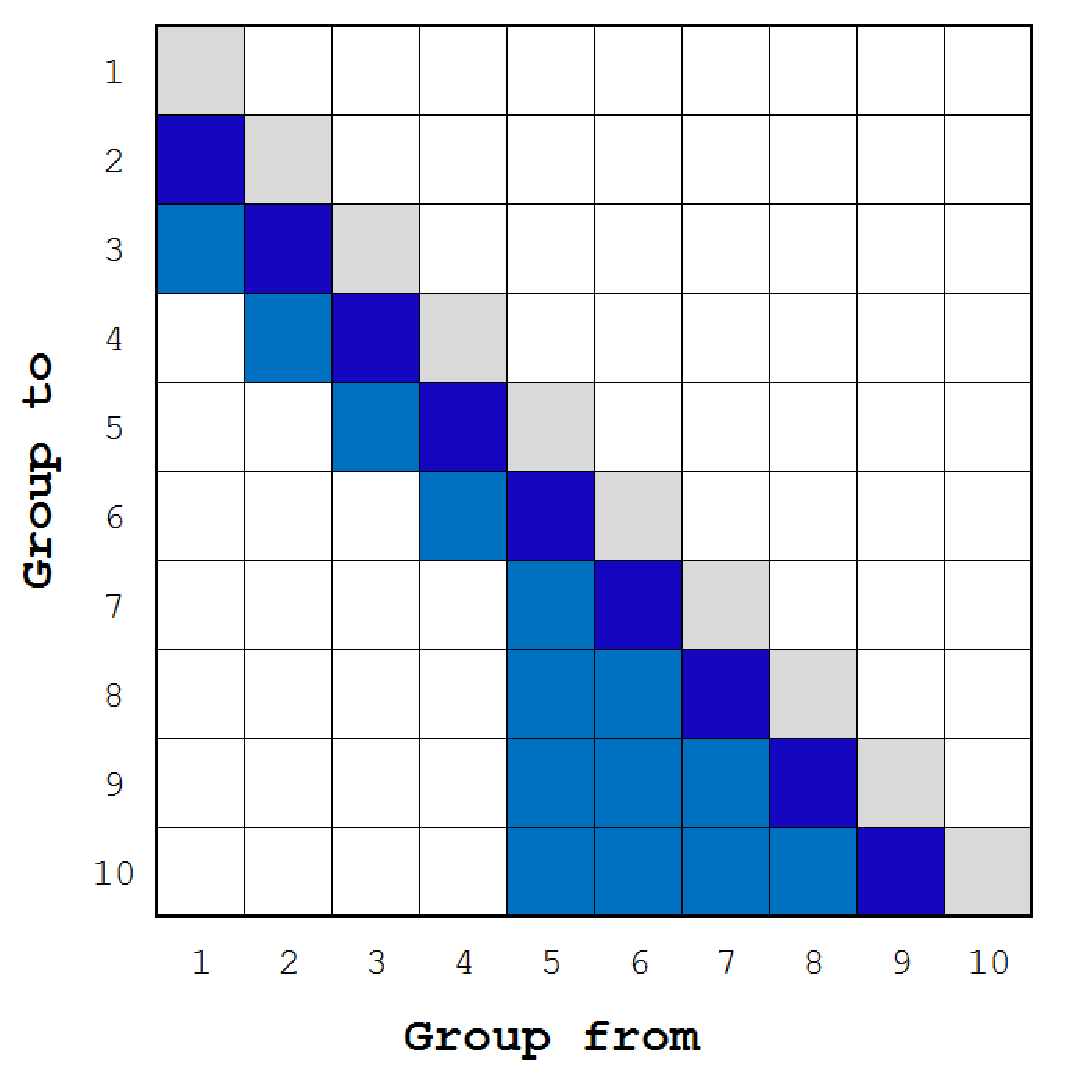
\includegraphics[width=\textwidth]{figures/sec_Sn/scattering_matrix_NO_upscattering.eps}
		\vspace{4mm}
	\end{subfigure}
	\hfill
	\begin{subfigure}[b]{0.58\textwidth}
		\centering
		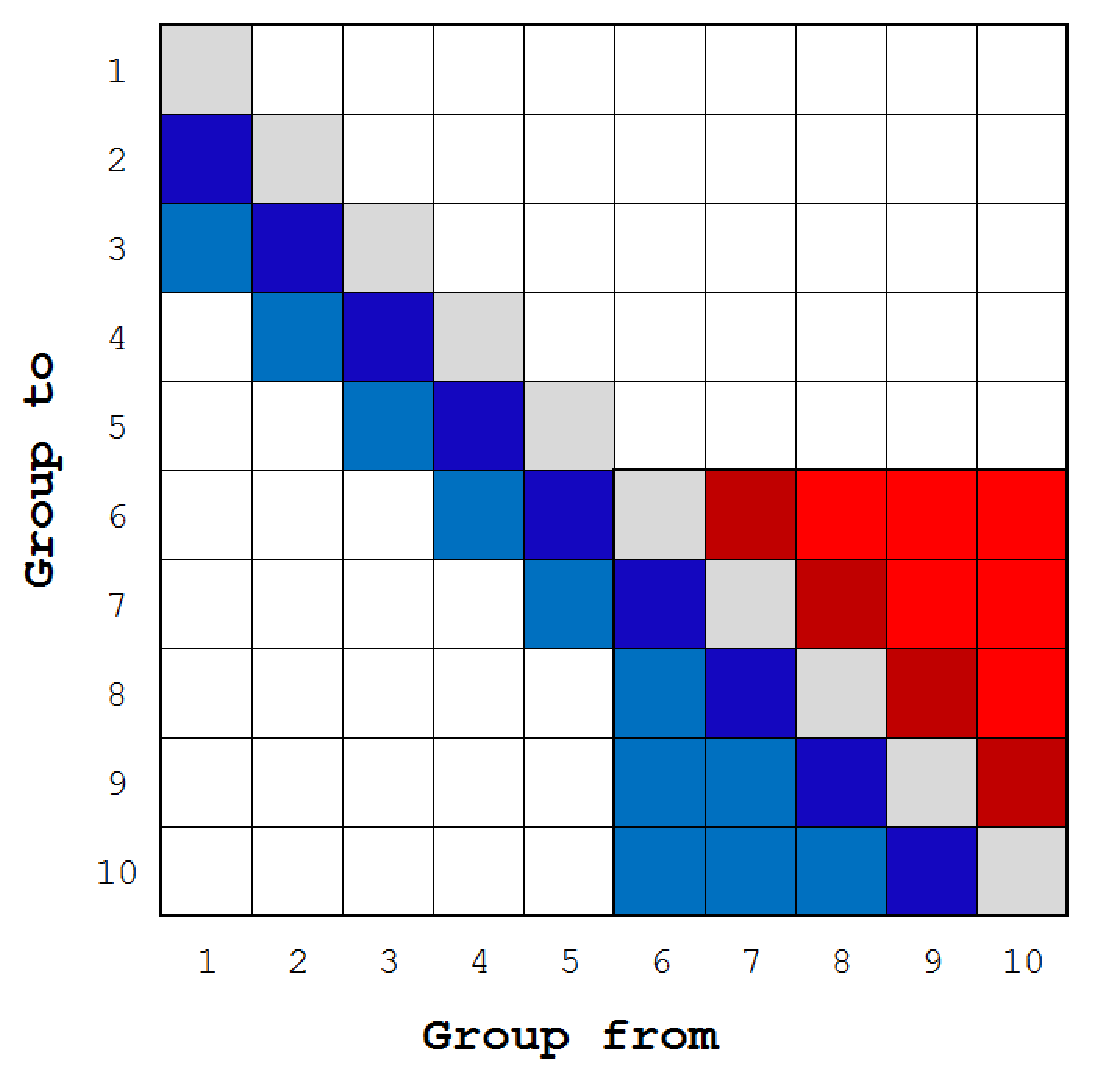
\includegraphics[width=\textwidth]{figures/sec_Sn/scattering_matrix_w_upscattering.eps}
	\end{subfigure}
\caption[Scattering matrices with and without upscattering]{Scattering matrices (top) without and (bottom) with upscattering. The gray corresponds to within-group scattering; the blue corresponds to down-scattering in energy; and the red corresponds to up-scattering in energy.}
\label{fig::Sn_Solution_Iterative_scattmatrix}
\end{figure}

\begin{equation}
\label{eq::Sn_full_sol_ops}
\begin{aligned}
{\bf L} {\bf \Psi} - {\bf M} {\bf \Sigma} {\bf \Phi}  =    {\bf Q} \\
{\bf \Phi} =  {\bf D} {\bf \Psi}
\end{aligned}
\end{equation}

\noindent where ${\bf L}$ is the fully-discretized loss operator which consists of total interaction and streaming terms, ${\bf M}$ is the moment-to-discrete operator of the angular discretization, ${\bf D}$ is the discrete-to-moment operator of the angular discretization, ${\bf \Sigma}$ is the scattering operator of the multigroup and angular discretizations, and ${\bf Q}$ is the full phase-space distributed source. In this case the source contains contributions from boundary and domain sources, fission sources, and scattering sources from outside the group set into the group set of interest.



\begin{equation}
\label{eq::Sn_full_sol_moments_only}
\left[ {\bf I} - {\bf D} {\bf L}^{-1}{\bf M} {\bf \Sigma}   \right] {\bf \Phi} =  {\bf D} {\bf L}^{-1}  {\bf Q} 
\end{equation}

\noindent where we define,

\begin{equation}
\label{eq::Sn_trans_op_T}
{\bf T} \equiv {\bf D} {\bf L}^{-1}{\bf M} {\bf \Sigma} ,
\end{equation}

\noindent for further brevity.



%%%%%%%%%%%%%%%%%%%%%%%%%%%%%%%%%%%%%%%%%%%%%%%%%%%
%%%   SubSubSection - Source Iteration
\subsubsection{Source Iteration}
\label{sec::Sn_Solution_Iterative_SI}

One simple method to invert $({\bf I} - {\bf T})$ of Eq. (\ref{eq::Sn_full_sol_moments_only}) is the {\em source iteration} technique, also known as {\em richardson iteration}.

\begin{equation}
\label{eq::Sn_si_iter}
\begin{aligned}
 {\bf \Psi}^{(\ell+1)} = {\bf L}^{-1}  {\bf M} {\bf \Sigma} {\bf \Phi}^{(\ell)} + {\bf L}^{-1}  {\bf Q} \\
{\bf \Phi}^{(\ell+1)} =  {\bf D} {\bf \Psi}^{(\ell+1)}
\end{aligned}
\end{equation}

%%%%%%%%%%%%%%%%%%%%%%%%%%%%%%%%%%%%%%%%%%%%%%%%%%%
%%%   SubSubSection - Source Iteration
\subsubsection{Krylov Subspace Methods - GMRES}
\label{sec::Sn_Solution_Iterative_GMRES}

%%%%%%%%%%%%%%%%%%%%%%%%%%%%%%%%%%%%%%%%%%%%%%%%%%%
%%%   SubSection - Spatial Solution Procedures
\subsection{Spatial Solution Procedures}
\label{sec::Sn_Solution_Spatial}

Section \ref{sec::Sn_Solution_Iterative} presented the methodology that we will employ to iteratively converge our transport solutions in energy and angle (flux moments). Both richardson iteration and GMRES were presented as methods that can invert the $({\bf I} - {\bf T})$ operator. In both of these iterative methods, the common operation of interest is the inversion of the loss operator (${\bf L}$). There are different techniques that could be used to perform this operation, including serveral matrix-dependent and matrix-free methodologies. For this work, we will utilize the full-domain transport sweep as we outline next in Section \ref{sec::Sn_Solution_Spatial_Sweeping}.

%%%%%%%%%%%%%%%%%%%%%%%%%%%%%%%%%%%%%%%%%%%%%%%%%%%
%%%   SubSubSection - Transport Sweeping
\subsubsection{Transport Sweeping}
\label{sec::Sn_Solution_Spatial_Sweeping}

The full-domain transport sweep is a beneficial matrix-free scheme because of the following:

\begin{itemize}
\item The number of sweep iterations does not grow with increasing problem size or processor counts. This is in contrast with partial-domain sweeping like {\em parallel block jacobi} (PBJ) \cite{zerr2011solution}.
\item Does not require the formation of $M$ separate matrices for each of the angular directions. 
\item 
\end{itemize}

\begin{figure}
\centering
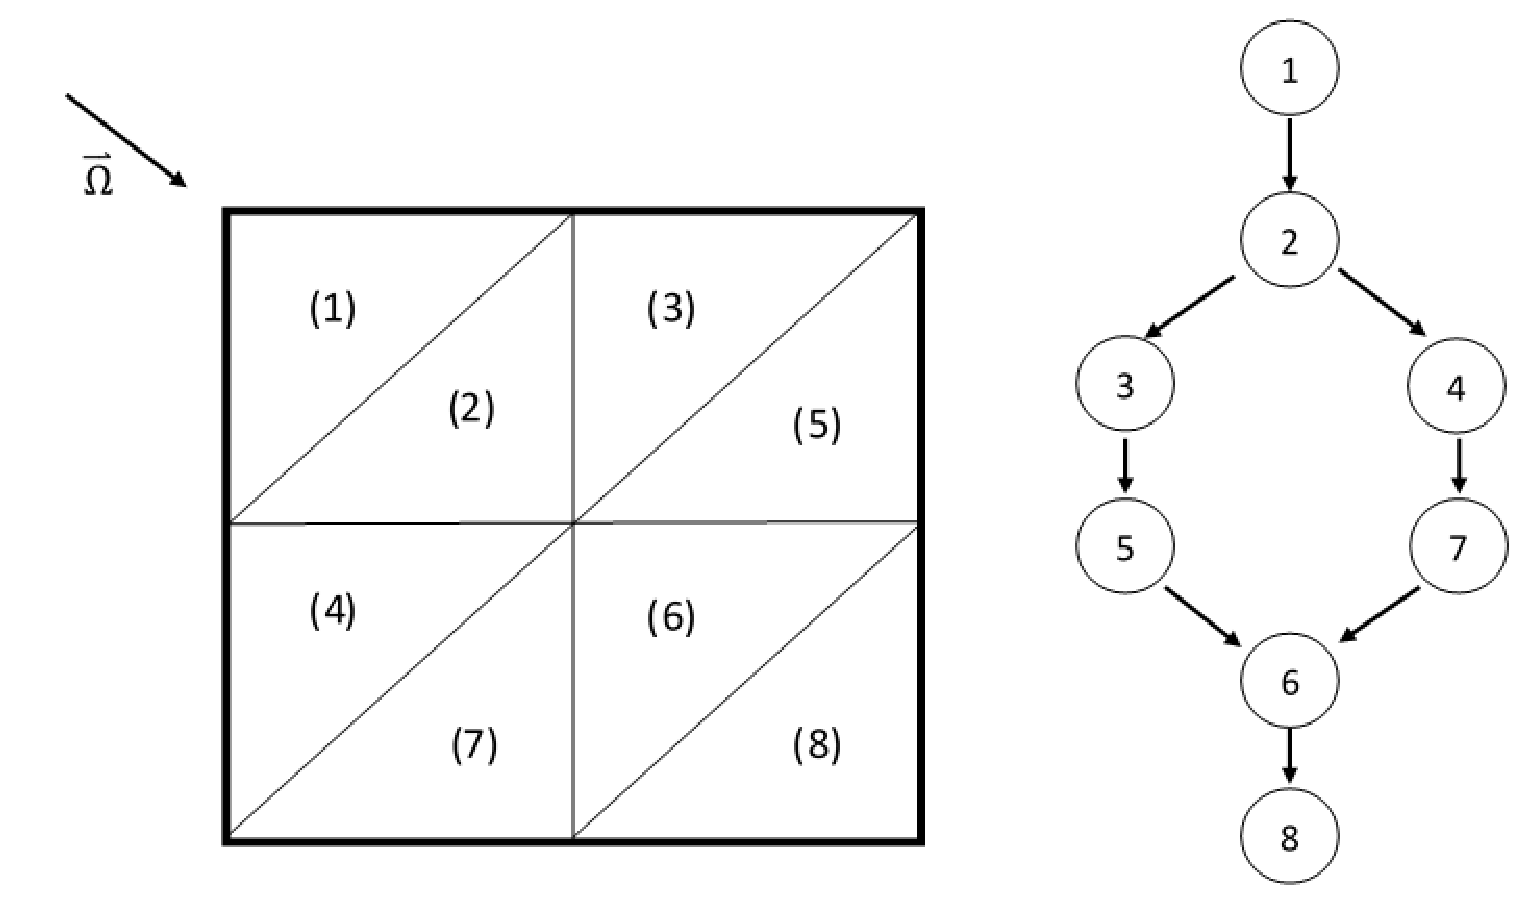
\includegraphics[width=0.75\textwidth]{figures/sec_Sn/triangle_graph_nocycle.eps}
\caption[blah]{blah.}
\label{fig::Sn_Solution_Spatial_Sweeping_sweepNOcycle}
\end{figure}

\begin{figure}
\centering
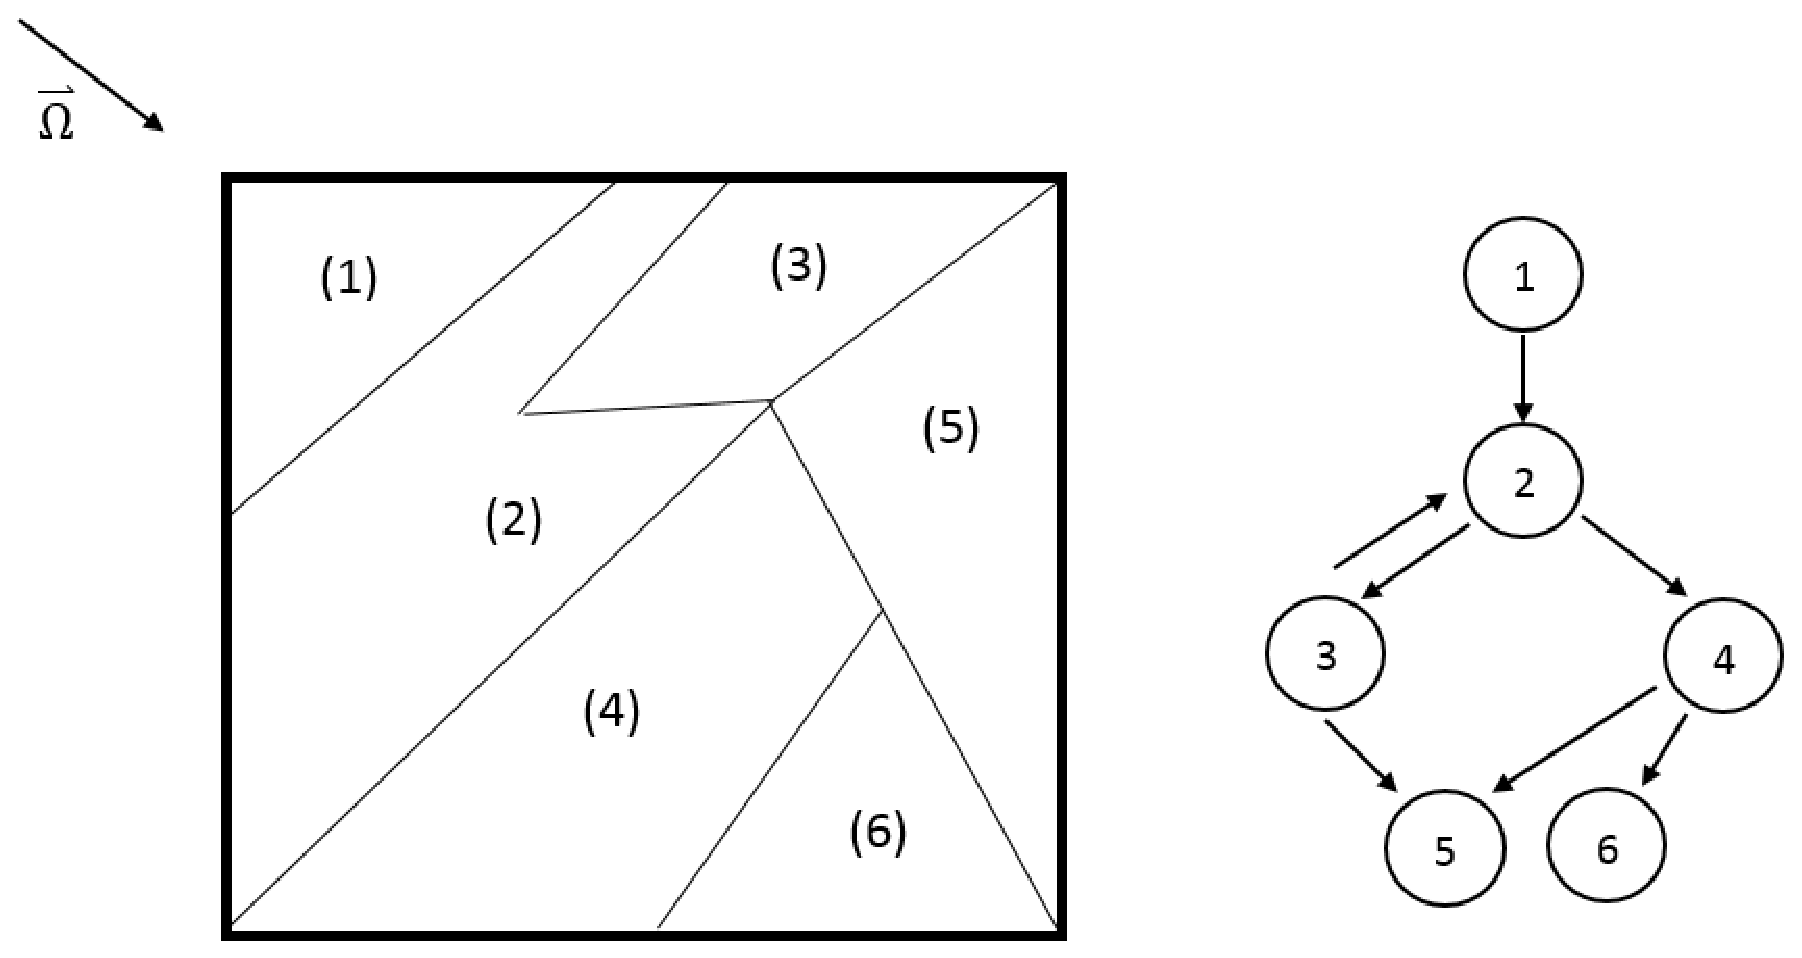
\includegraphics[width=0.75\textwidth]{figures/sec_Sn/graph_with_cycling.eps}
\caption[blah]{blah.}
\label{fig::Sn_Solution_Spatial_Sweeping_sweepWcycle}
\end{figure}

%%%%%%%%%%%%%%%%%%%%%%%%%%%%%%%%%%%%%%%%%%%%%%%%%%%
%%%   SubSubSection - AMR
\subsubsection{Adaptive Mesh Refinement}
\label{sec::Sn_Solution_Spatial_AMR}

\begin{equation}
\label{eq::Sn_AMR_jump_err_est}
\eta_K^r = \int\displaylimits_{\partial K} [\![ \Phi^r ]\!]^2 d \, s = \int\displaylimits_{\partial K} \left(  \sum_m w_m [\![ \Psi_m^r ]\!]  \right)^2
\end{equation}

\noindent where $[\![ \cdot ]\!]$ is the jump operator along a face defined as,

\begin{equation}
\label{eq::Sn_AMR_jump_def}
[\![ \Phi (\vec{r}) ]\!] = \Phi^+ (\vec{r}) - \Phi^- (\vec{r}),
\end{equation}

\noindent and the terms,$\Phi^+ (\vec{r})$ and $\Phi^- (\vec{r})$, are subject to the trace:

\begin{equation}
\label{eq::Sn_AMR_jump_trace}
\Phi^{\pm} (\vec{r})  = \lim\displaylimits_{s \rightarrow 0^{\pm}} \Phi (\vec{r} + s \vec{n}).
\end{equation}

\noindent In this case, the outward normal, $\vec{n}$, is determined with respect to the element $K$ along its boundary, $\partial K$. With this trace, $\Phi^- (\vec{r})$ always corresponds to the solution within cell $K$. Investigating face $f$ of cell $K$, the across-face solution, $\Phi^+ (\vec{r})$, is dependent on the boundary type of face $f$. The across-face solutions can be succinctly writen:

\begin{equation}
\label{eq::Sn_AMR_across_face_vals}
\Phi^+ (\vec{r}) = 
\begin{cases}
\lim\displaylimits_{s \rightarrow 0^{+}} \Phi (\vec{r} + s \vec{n}) & \vec{r} \notin \partial \mathcal{D} \\
\sum\displaylimits_{\vec{\Omega}_m \cdot \vec{n} > 0}  \Psi_m^- (\vec{r}) + \sum\displaylimits_{\vec{\Omega}_m \cdot \vec{n} < 0} \Psi_{m}^{inc} (\vec{r}) & \vec{r} \in \partial \mathcal{D}^d \\
\Phi^- (\vec{r}) & \vec{r} \in \partial \mathcal{D}^r
\end{cases}.
\end{equation}

\noindent From Eq. (\ref{eq::Sn_AMR_across_face_vals}), the across-face solutions for interior faces, incident boundaries and reflecting boundaries have different meanings. For an interior face $f$ ($\vec{r} \notin \partial \mathcal{D}$), the across-face solution comes from the cell $K'$ (as defined by Figure \ref{fig::Sn_two_ref_cells}). For incident boundaries ($\vec{r} \in \partial \mathcal{D}^d$), the across-face solution is a combination of integrals of the outgoing ($\Psi_m^-$) and incident boundary fluxes ($\Psi_m^{inc}$). Finally, for reflecting boundaries ($\vec{r} \in \partial \mathcal{D}^r$), the across-face solutions are simply the within-cell solutions. Therefore, the solution jump is exactly zero for all reflecting boundaries and yields no contribution to the error estimate.

\begin{equation}
\label{eq::Sn_AMR_err_crit}
\eta_K^r \geq \alpha \max\displaylimits_{K' \in \mathbb{T}_h^r} \left(  \eta_{K'}^{r} \right)
\end{equation}

\noindent where $\alpha$ is a user-defined value $(0,1)$. This refinement criterion has a simple meaning. If, for example, $\alpha = 0.2$, then a cell will be refined if its error estimate is greater than 20\% of the cell with the largest error estimate. This does not necessarily mean that 80\% of the mesh cells will be refined at level $r$. Instead, the criterion simply states that any cell above a particular threshold will be refined. This means that it is theoretically possible for the extreme cases of 1 or all cells being refined at a particular refinement cycle.


%%%%%%%%%%%%%%%%%%%%%%%%%%%%%%%%%%%%%%%%%%%%%%%%%%%
%%%   Section - Conclusions
\section{Conclusions}
\label{sec::Sn_Conclusions}

In this chapter, we have presented the tightly-coupled system of equations that comprise the DGFEM $S_N$ transport equation. We began with the fully-continuous transport equation presented in Section \ref{sec::Sn_neut} and then discretized it in energy, angle and space in Sections \ref{sec::Sn_MG}, \ref{sec::Sn_Angle}, and \ref{sec::Sn_Spatial}, respectively. Appropriate boundary conditions were presented in Section \ref{sec::Sn_BC}. For this work, we will only utilize incoming-incident and reflecting boundary conditions and not use any further albedo terms. We finished this chapter in Section \ref{sec::Sn_Solution} by describing the procedures that will be utilized to solve our system of equations.


%%%%%%%%%%%%%%%%%%%%%%%%%%%%%%%%%%%%%%%%%%%%%%%%%%%
%
%  New template code for TAMU Theses and Dissertations starting Fall 2012.  
%  For more info about this template or the 
%  TAMU LaTeX User's Group, see http://www.howdy.me/.
%
%  Author: Wendy Lynn Turner 
%	 Version 1.0 
%  Last updated 8/5/2012
%
%%%%%%%%%%%%%%%%%%%%%%%%%%%%%%%%%%%%%%%%%%%%%%%%%%%
%%%                           SECTION V
%%%%%%%%%%%%%%%%%%%%%%%%%%%%%%%%%%%%%%%%%%%%%%%%%%%
\chapter{\uppercase {FEM Basis Functions for Unstructured Polytopes}}
\label{sec::BF}

In Section \ref{sec::Sn_Spatial}, we detailed the spatial discretization of the transport equation. We then proceeded to give the functional forms for the various elementary matrices needed to form the full set of spatially-discretized PDEs. These included the mass, streaming, and surface matrices where the integrations on the element's domain and boundary require combinations of the basis functions' values and gradients.

%%%%%%%%%%%%%%%%%%%%%%%%%%%%%%%%%%%%%%%%%%%%%%%%%%%
%%%   Section - 2D Linear
\section{Linear Basis Functions on 2D Polygons}
\label{sec::BF_2DLinear}

Figure \ref{fig::BF_2D_ref_polygon}, gives an image of a reference polygon along with the geometric notations we will use to define the different linear polygonal coordinates. An element, $K\in \mathbb{R}^2$, is defined by a closed set of $N_K$ points (vertices) in $\mathbb{R}^2$. The vertices are ordered ($1,...,N_K$) in a counter-clockwise manner without restriction on their convexity. Face $j$ on the polygon, $e_j$, is defined as the line segment between vertices $j$ and $j+1$. The vertex $j+1$ is determined in general as $j+1 =\mod(j,N_K)+1$, which gives a wrap-around definition of vertex $N_K+1 = 1$.

We complete our geometric description for the polygonal coordinate system by analyzing a point $\vec{x}$ inside the polygon's domain, as also seen in Figure \ref{fig::BF_2D_ref_polygon}. $\alpha_j$ is the angle between the points ($\vec{x}_j, \vec{x}, \vec{x}_{j+1}$). Since element $K$ is defined by a closed set of $\mathbb{R}^2$ points, $\alpha_j$ is strongly bounded: ($[0, \pi]$). We conclude by defining $|\vec{u}|$ as the Euclidean distance of the vector $\vec{u}$. This means that $|\vec{x} - \vec{x}_j|$ is the distance between the points $\vec{x}$ and $\vec{x}_j$ and $|e_j|$ is the length of face $j$ between points $\vec{x}_j$ and $\vec{x}_{j+1}$.

\begin{figure}[hbt]
\centering
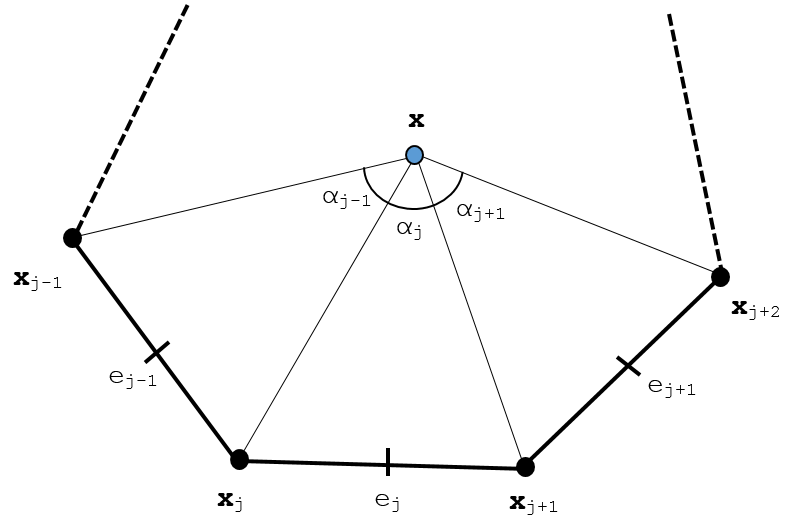
\includegraphics[width=0.65\textwidth]{figures/sec_BF/ref_polygon.png}
\caption{Arbitrary polygon with geometric properties used for 2D basis function generation.}
\label{fig::BF_2D_ref_polygon}
\end{figure}

In this dissertation, all 1st-order, two-dimensional basis functions for a cell will obey the properties for barycentric coordinates. They will form a {\em partition of unity},

\begin{equation}
\sum_{i=1}^{N_K} b_i (\vec{x})  =  1;
\label{eq::BF_linear_interp_partition}
\end{equation}

\noindent coordinate interpolation will result from an {\em affine combination} of the vertices,

\begin{equation}
\sum_{i=1}^{N_K} b_i(\vec{x}) \vec{x}_i  =  \vec{x};
\label{eq::BF_linear_interp_affine}
\end{equation}

\noindent and they will satisfy the {\em Lagrange property},

\begin{equation}
b_i (\vec{x}_j) = \delta_{ij}.
\label{eq::BF_linear_interp_lagrange}
\end{equation}

\noindent $N_K$ is again the number of spatial degrees with measure in element $K$. Using the {\em partition of unity} of Eq. (\ref{eq::BF_linear_interp_partition}), we can rewrite Eqs. (\ref{eq::BF_linear_interp_partition}-\ref{eq::BF_linear_interp_affine}) into a separate, compact, vectorized form for completeness

\begin{equation}
\sum_{i=1}^{N_K}  b_i (\vec{x}) \vec{c}_{i,1}(\vec{x}) = \vec{q}_1 ,
\label{eq::BF_linear_interp_req_vector}
\end{equation}

\noindent where $\vec{c}_{i,1}(\vec{x})$ and $\vec{q}_1$ are the lineary-complete constraint and equivalence terms, respectively. These terms are simply:

\begin{equation}
\vec{c}_{i,1}(\vec{x}) = \left[
\begin{array}{c}
1 \\
x_i - x \\
y_i - y
\end{array} \right]
  \qquad \text{and} \qquad \vec{q}_1 = \left[
\begin{array}{c}
1 \\
0 \\
0
\end{array} \right],
\label{eq::BF_linear_constraint_terms}
\end{equation}

\noindent respectively.

%%%%%%%%%%%%%%%%%%%%%%%%%%%%%%%%%%%%%%%%%%%%%%%%%%%
%%%   SubSection - Linear
\subsection{Traditional Linear Basis Functions - $\mathbb{P}_{1}$ and $\mathbb{Q}_{1}$ Spaces}
\label{sec::BF_2DLinear_LDandBLD}

Before presenting basis function sets applicable to polytope finite elements, we first provide two common basis functions that are exact on triangles and convex quadrilaterals: the $\mathbb{P}_{1}$ and $\mathbb{Q}_{1}$ spaces, respectively. 

\begin{equation}
\label{eq::2D_lin_basis_functions}
\begin{aligned}
	b_1(r,s) & = 1-r-s \\
	b_2(r,s) & = r \\
	b_3(r,s) & = s 
\end{aligned}
\end{equation}

\noindent 

and

\begin{equation}
\label{eq::BiL_basis_functions}
\begin{aligned}
	b_1(r,s) & = (1-r)(1-s) \\
	b_2(r,s) & = r(1-s) \\
	b_3(r,s) & = rs \\
	b_4(r,s) & = (1-r)s
\end{aligned}
\end{equation}


%%%%%%%%%%%%%%%%%%%%%%%%%%%%%%%%%%%%%%%%%%%%%%%%%%%
%%%   SubSection - Wachspress
\subsection{Wachspress Rational Basis Functions}
\label{sec::BF_2DLinear_Wachspress}

\begin{equation}
\label{eq::BF_wach_BF}
b_{j}^{W} (\vec{x}) = \frac{w_j (\vec{x}) }{\sum_i w_i (\vec{x})}
\end{equation}

\noindent where the Wachspress weight function for vertex $j$, $w_j$, has the following definition:

\begin{equation}
\label{eq::BF_wach_weights}
w_j (\vec{x})  = \frac{A(\vec{x}_{j-1}, \vec{x}_{j}, \vec{x}_{j+1})}{A(\vec{x}, \vec{x}_{j-1}, \vec{x}_{j}) \, A(\vec{x}, \vec{x}_{j}, \vec{x}_{j+1})}
\end{equation}

%%%%%%%%%%%%%%%%%%%%%%%%%%%%%%%%%%%%%%%%%%%%%%%%%%%
%%%   SubSection - PWL
\subsection{Piecewise Linear (PWL) Basis Functions}
\label{sec::BF_2DLinear_PWL}

\begin{equation}
\label{eq::PWL_2D}
	b_j^{PWL} (x,y) = t_j (x,y) + \alpha_j^K t_c (x,y)
\end{equation}

\noindent $t_j$ is the standard 2D linear function with unity at vertex $j$ that linearly decreases to zero to the cell center and each adjoining vertex. $t_c$ is the 2D cell ``tent'' function which is unity at the cell center and linearly decreases to zero to each cell vertex. $\alpha_{j}^{K}$ is the weight parameter for vertex $j$ in cell $K$. 



%%%%%%%%%%%%%%%
% Begin::2D PWL basis function plots
\pagebreak
\begin{figure}
\label{fig::2D_PWL_unit_square_basis_functions}
\centering
	\begin{subfigure}[b]{0.48\textwidth}
		\centering
		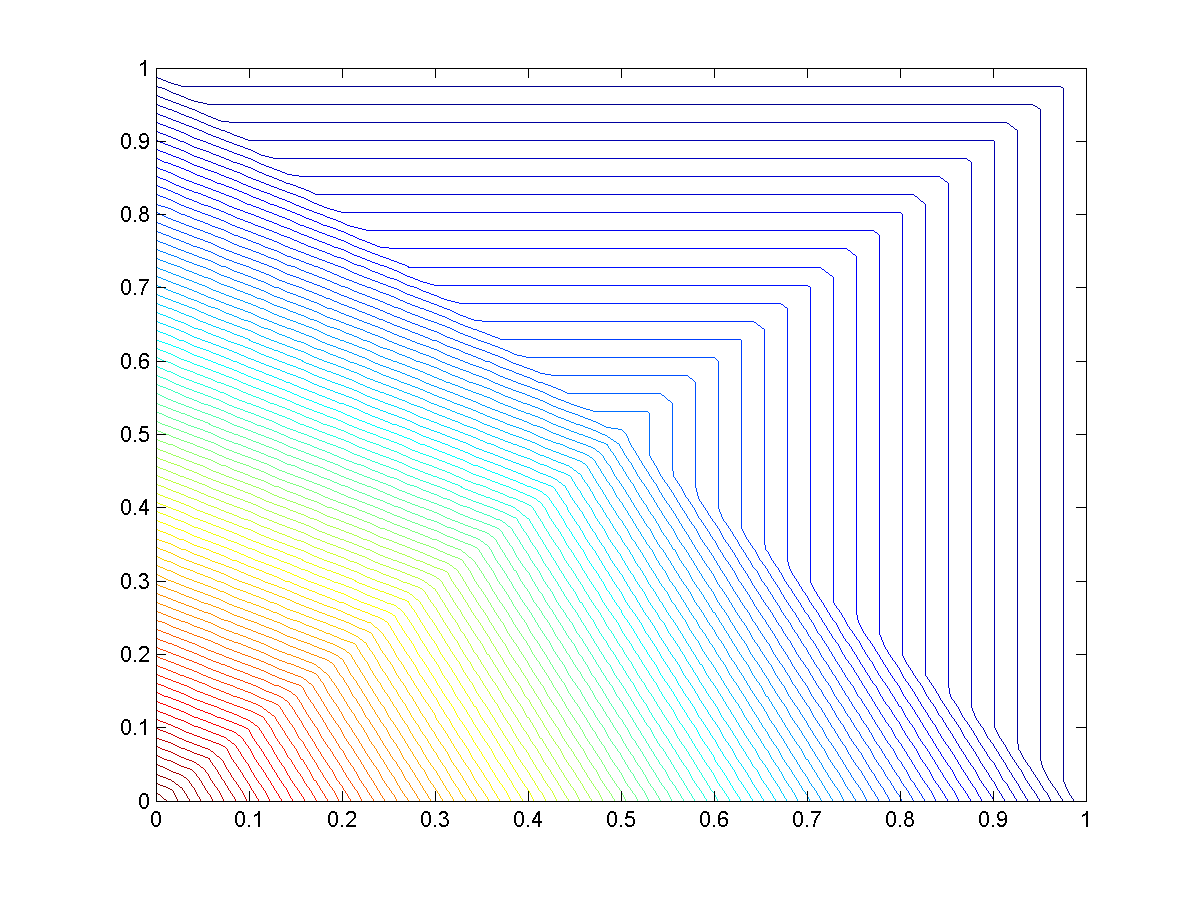
\includegraphics[width=\textwidth]{figures/sec_BF/PWL_square_contour_1.png}
		\caption{}
	\end{subfigure}
	\hfill
	\begin{subfigure}[b]{0.48\textwidth}
		\centering
		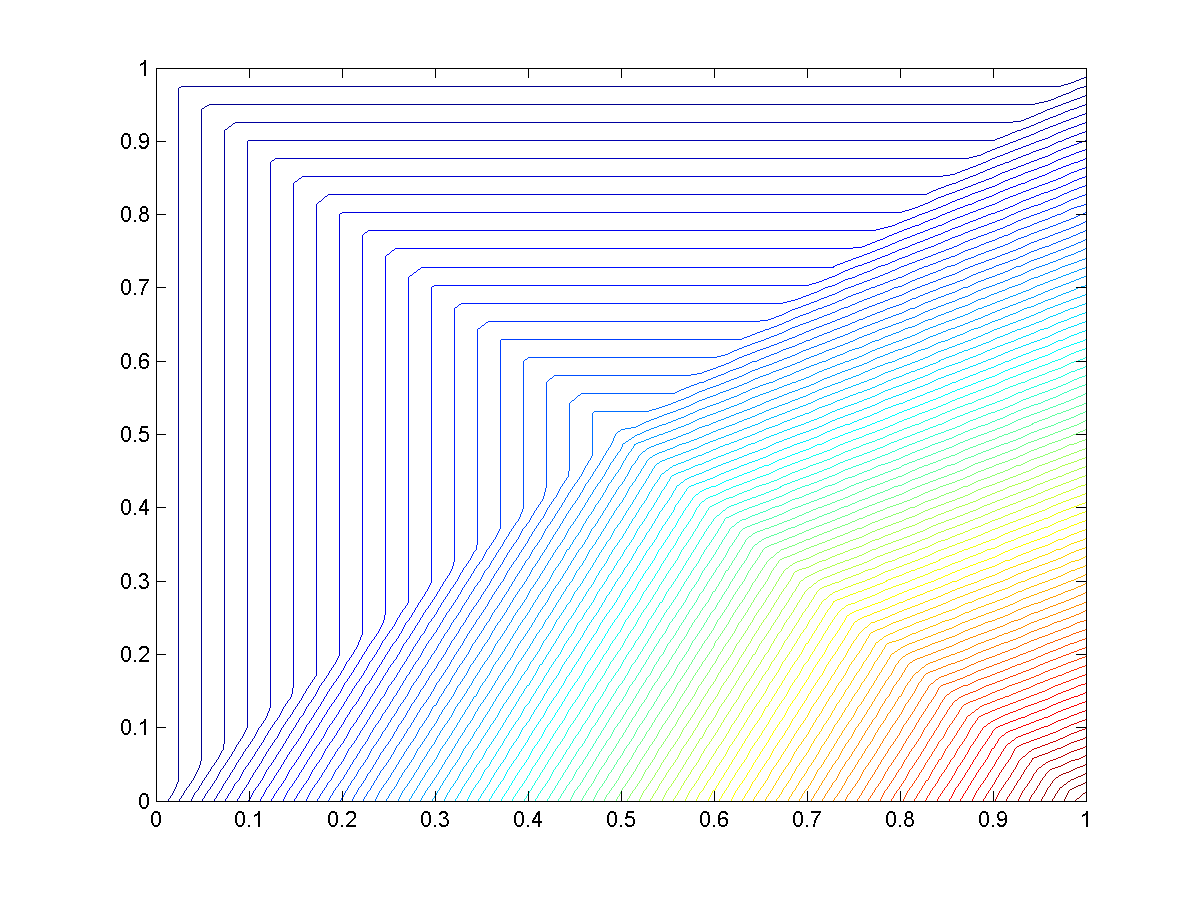
\includegraphics[width=\textwidth]{figures/sec_BF/PWL_square_contour_2.png}
		\caption{}
	\end{subfigure}
	\vfill
	\begin{subfigure}[b]{0.48\textwidth}
		\centering
		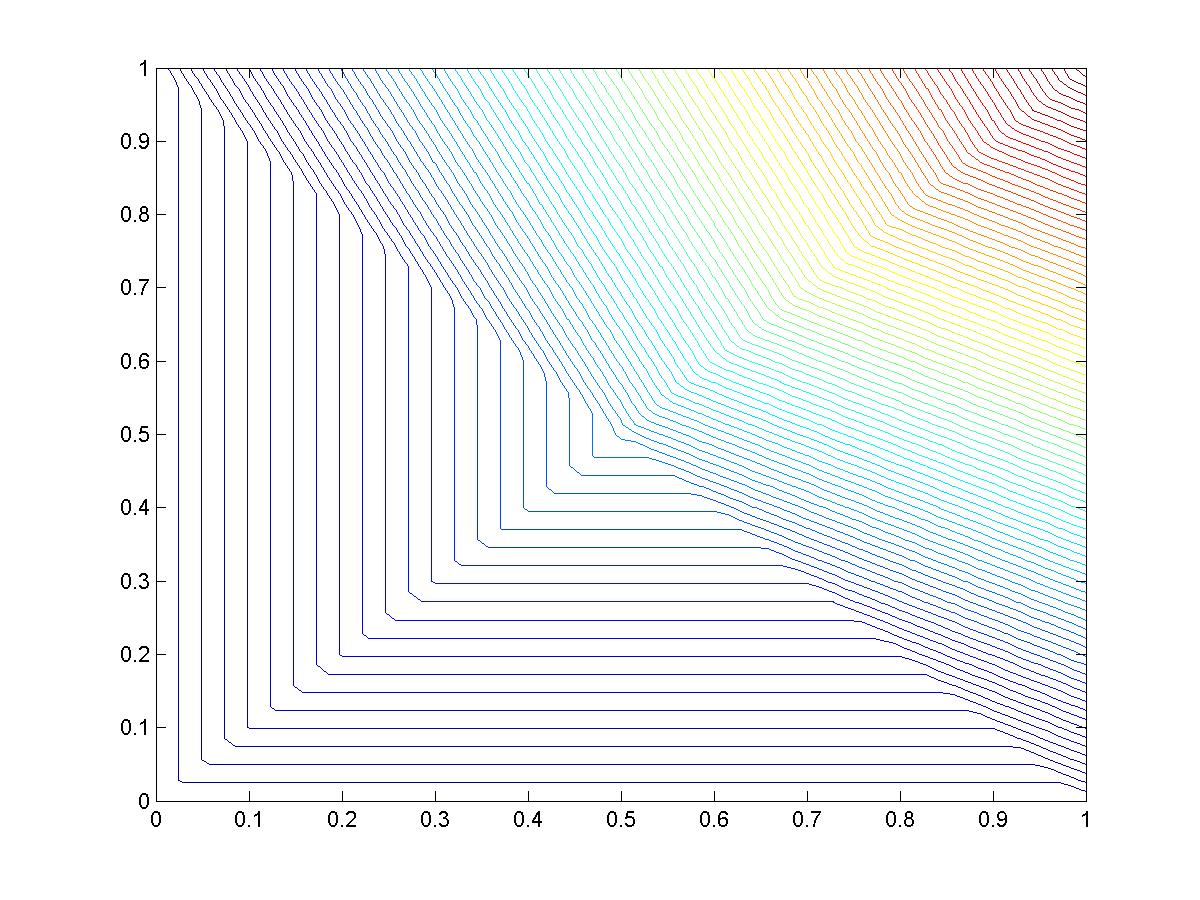
\includegraphics[width=\textwidth]{figures/sec_BF/PWL_square_contour_3.png}
		\caption{}
	\end{subfigure}
	\hfill
	\begin{subfigure}[b]{0.48\textwidth}
		\centering
		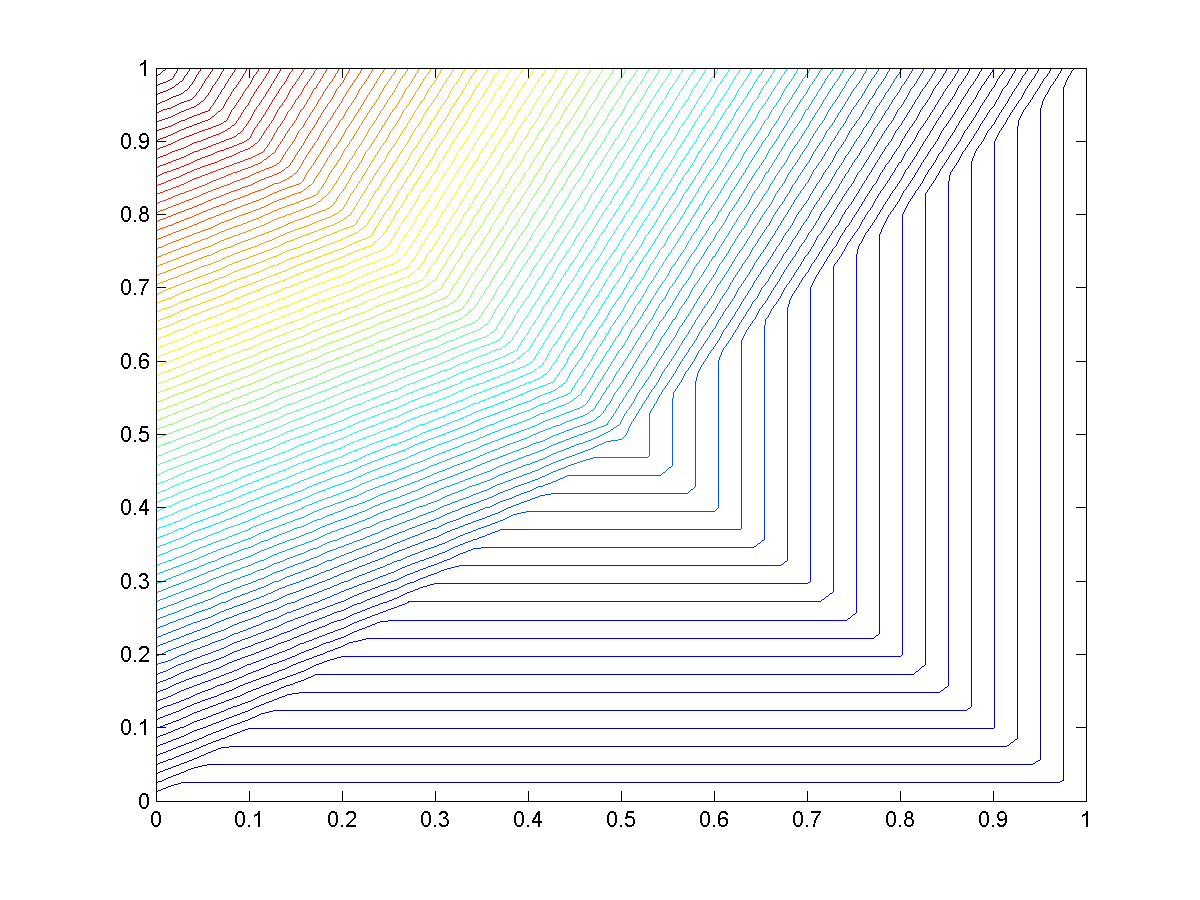
\includegraphics[width=\textwidth]{figures/sec_BF/PWL_square_contour_4.png}
		\caption{}
	\end{subfigure}
\caption{Contour plots of the PWL basis functions on the unit square for the vertices located at: (a) (0,0), (b) (1,0), (c) (1,1), and (d) (0,1).}
\end{figure}

\begin{figure}
\label{fig::2D_pentagon_vertices}
\centering
	\begin{subfigure}[b]{0.40\textwidth}
		\centering
		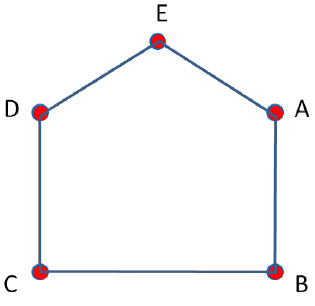
\includegraphics[width=\textwidth]{figures/sec_BF/reg_pent_verts.png}
		\caption{}
	\end{subfigure}
	\hfill
	\begin{subfigure}[b]{0.40\textwidth}
		\centering
		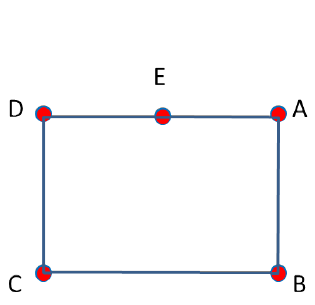
\includegraphics[width=\textwidth]{figures/sec_BF/deg_pent_verts.png}
		\caption{}
	\end{subfigure}
\caption{Vertex structure for a (a) regular pentagonal cell and a (b) degenerate pentagonal cell.}
\end{figure}

\begin{figure}
\label{fig::2D_PWL_pentagon_basis_functions_contour}
\centering
	\begin{subfigure}[b]{0.48\textwidth}
		\centering
		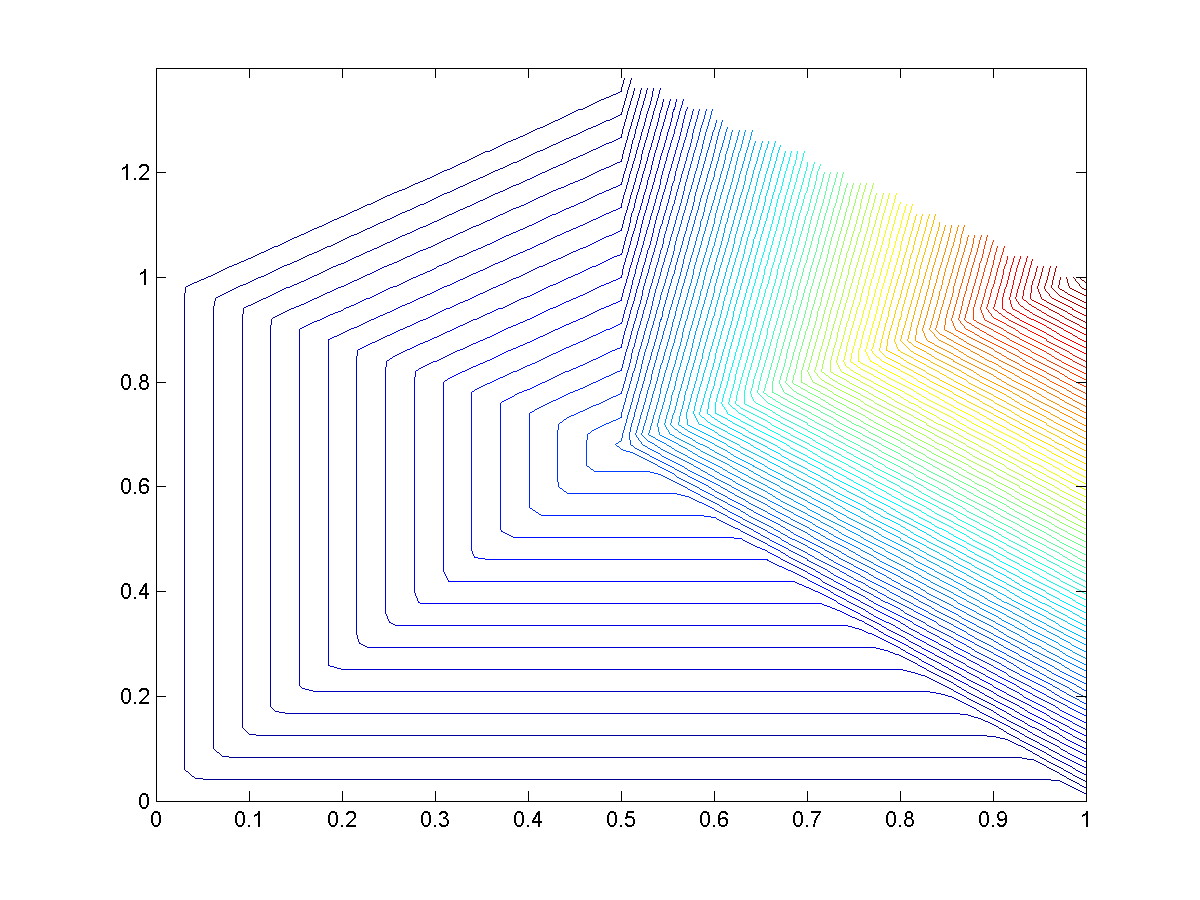
\includegraphics[width=\textwidth]{figures/sec_BF/PWL_rpent_contour_A.png}
		\caption{}
	\end{subfigure}
	\hfill
	\begin{subfigure}[b]{0.48\textwidth}
		\centering
		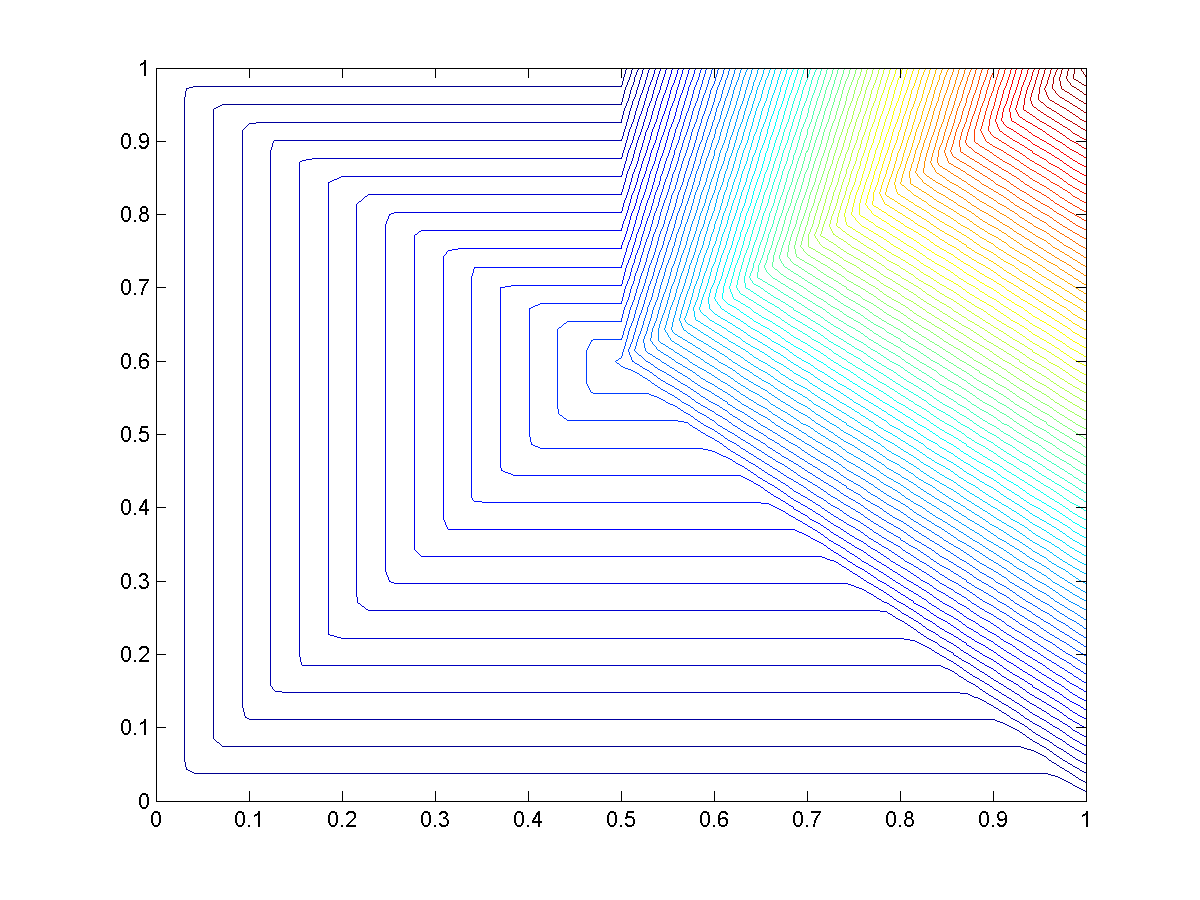
\includegraphics[width=\textwidth]{figures/sec_BF/PWL_dpent_contour_A.png}
		\caption{}
	\end{subfigure}
	\vfill
	\begin{subfigure}[b]{0.48\textwidth}
		\centering
		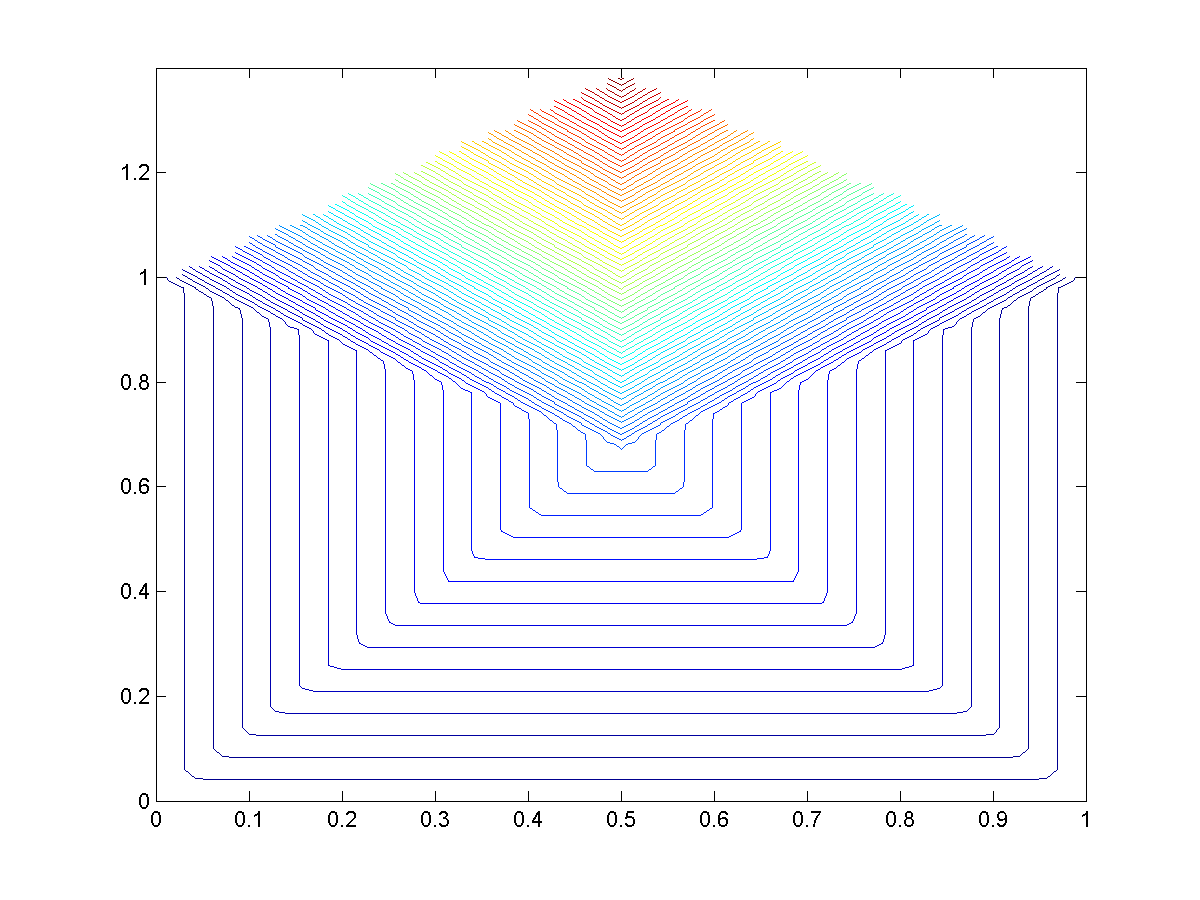
\includegraphics[width=\textwidth]{figures/sec_BF/PWL_rpent_contour_E.png}
		\caption{}
	\end{subfigure}
	\hfill
	\begin{subfigure}[b]{0.48\textwidth}
		\centering
		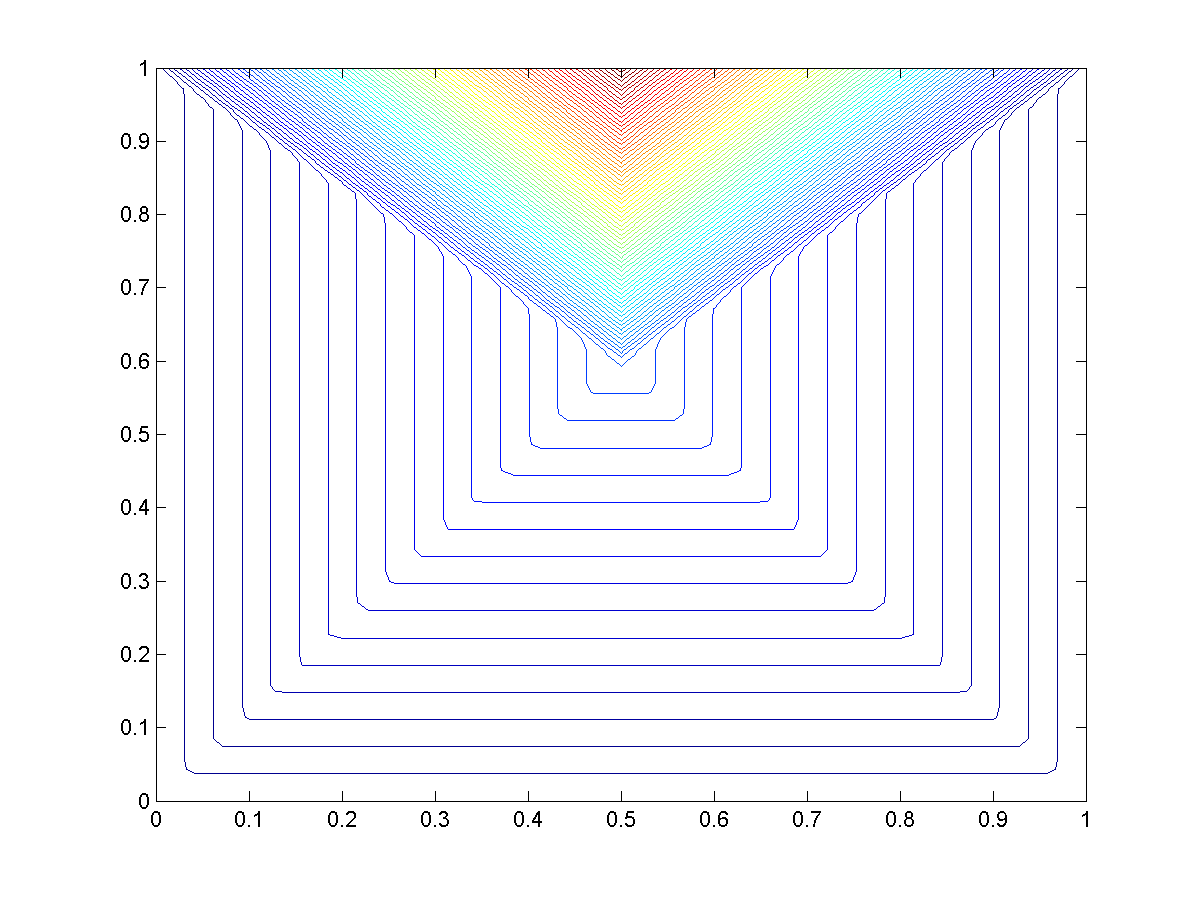
\includegraphics[width=\textwidth]{figures/sec_BF/PWL_dpent_contour_E.png}
		\caption{}
	\end{subfigure}
\caption{Contour plots of the PWL basis functions for a regular pentagon: (a) and (c) as well as a degenerate pentagon: (b) and (d).}
\end{figure}

\begin{figure}
\label{fig::2D_PWL_pentagon_basis_functions_plot}
\centering
	\begin{subfigure}[b]{0.48\textwidth}
		\centering
		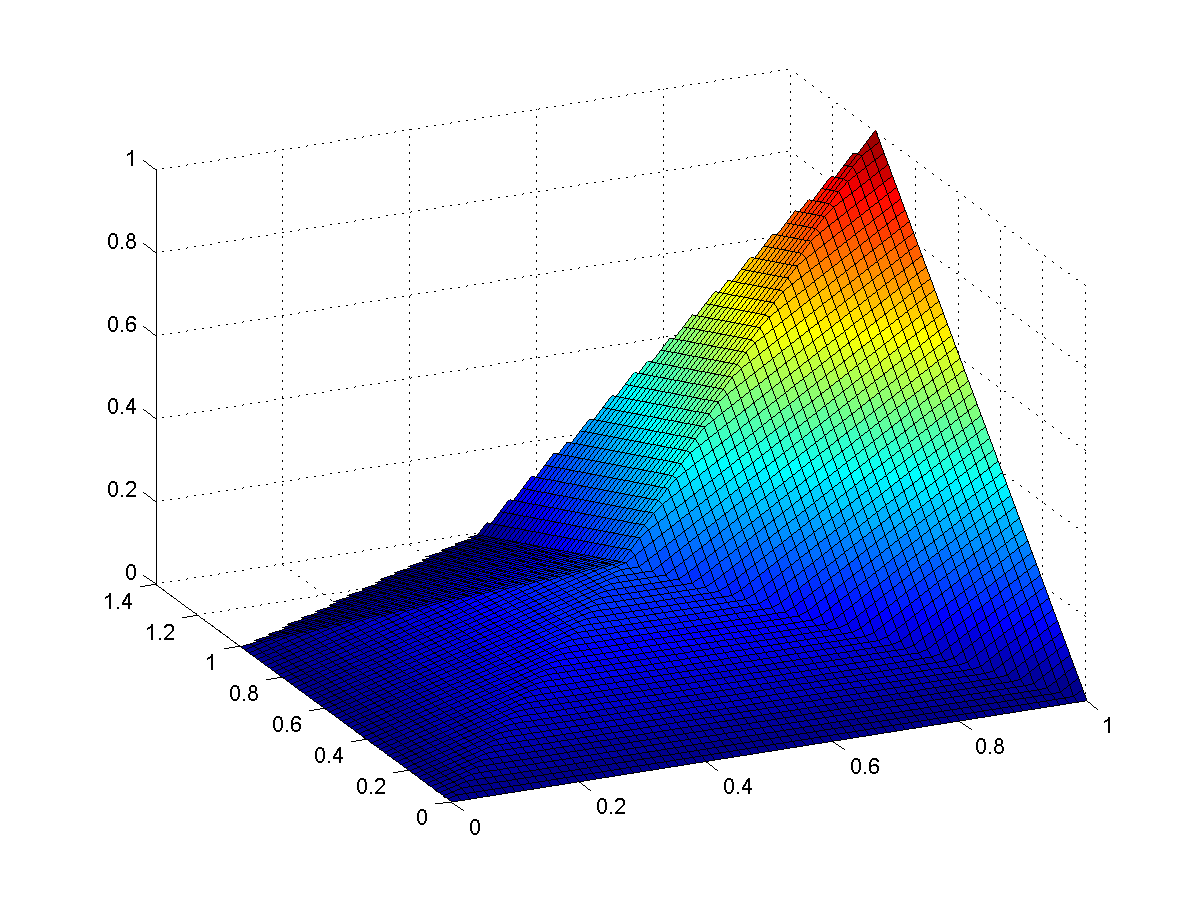
\includegraphics[width=\textwidth]{figures/sec_BF/PWL_rpent_plot_A.png}
		\caption{}
	\end{subfigure}
	\hfill
	\begin{subfigure}[b]{0.48\textwidth}
		\centering
		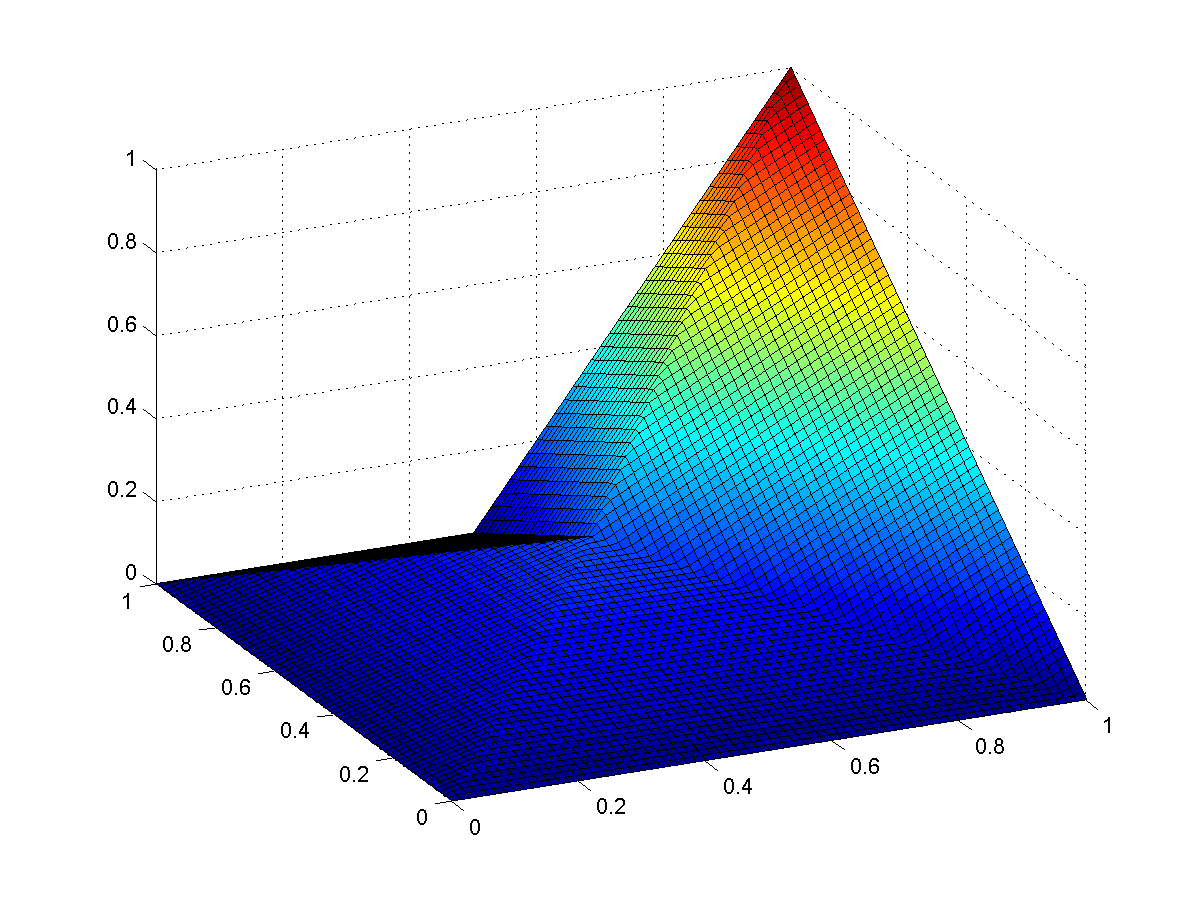
\includegraphics[width=\textwidth]{figures/sec_BF/PWL_dpent_plot_A.png}
		\caption{}
	\end{subfigure}
	\vfill
	\begin{subfigure}[b]{0.48\textwidth}
		\centering
		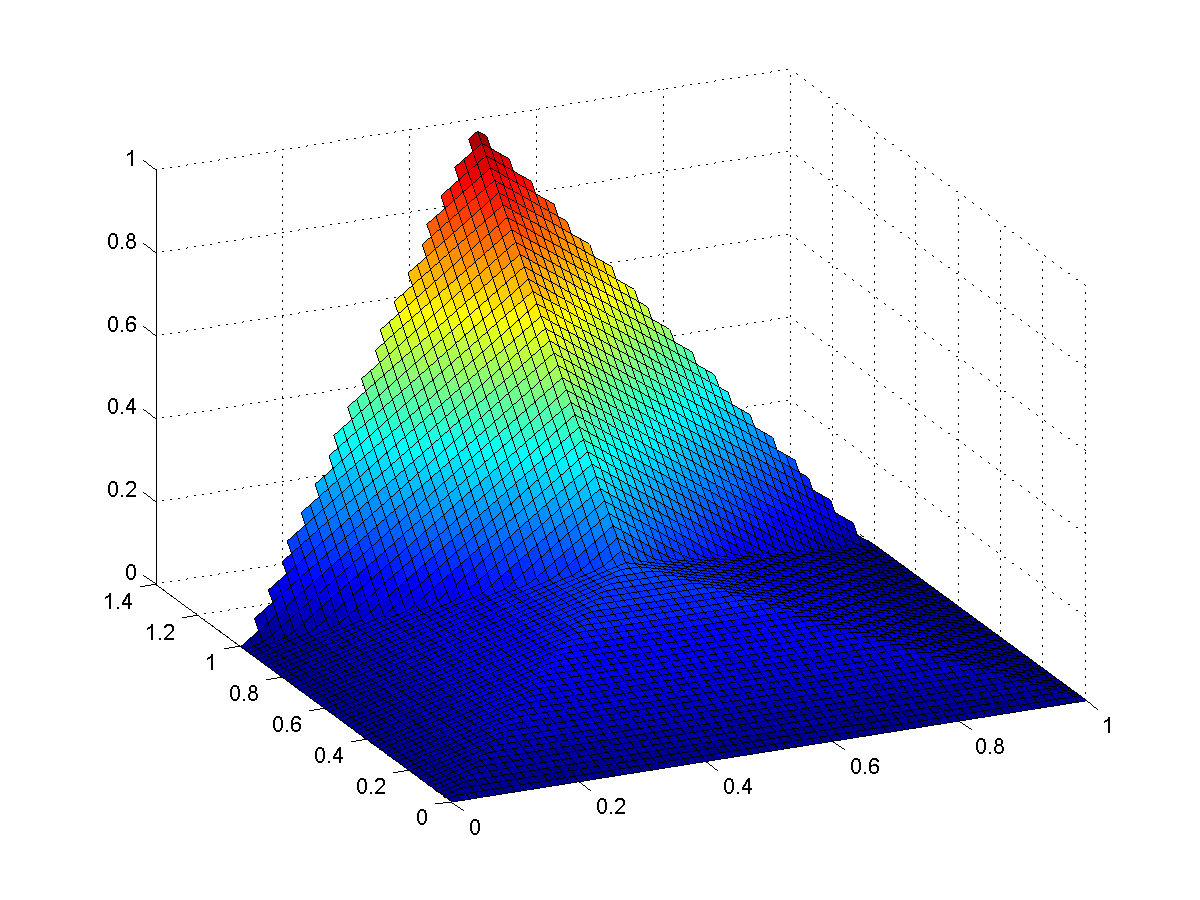
\includegraphics[width=\textwidth]{figures/sec_BF/PWL_rpent_plot_E.png}
		\caption{}
	\end{subfigure}
	\hfill
	\begin{subfigure}[b]{0.48\textwidth}
		\centering
		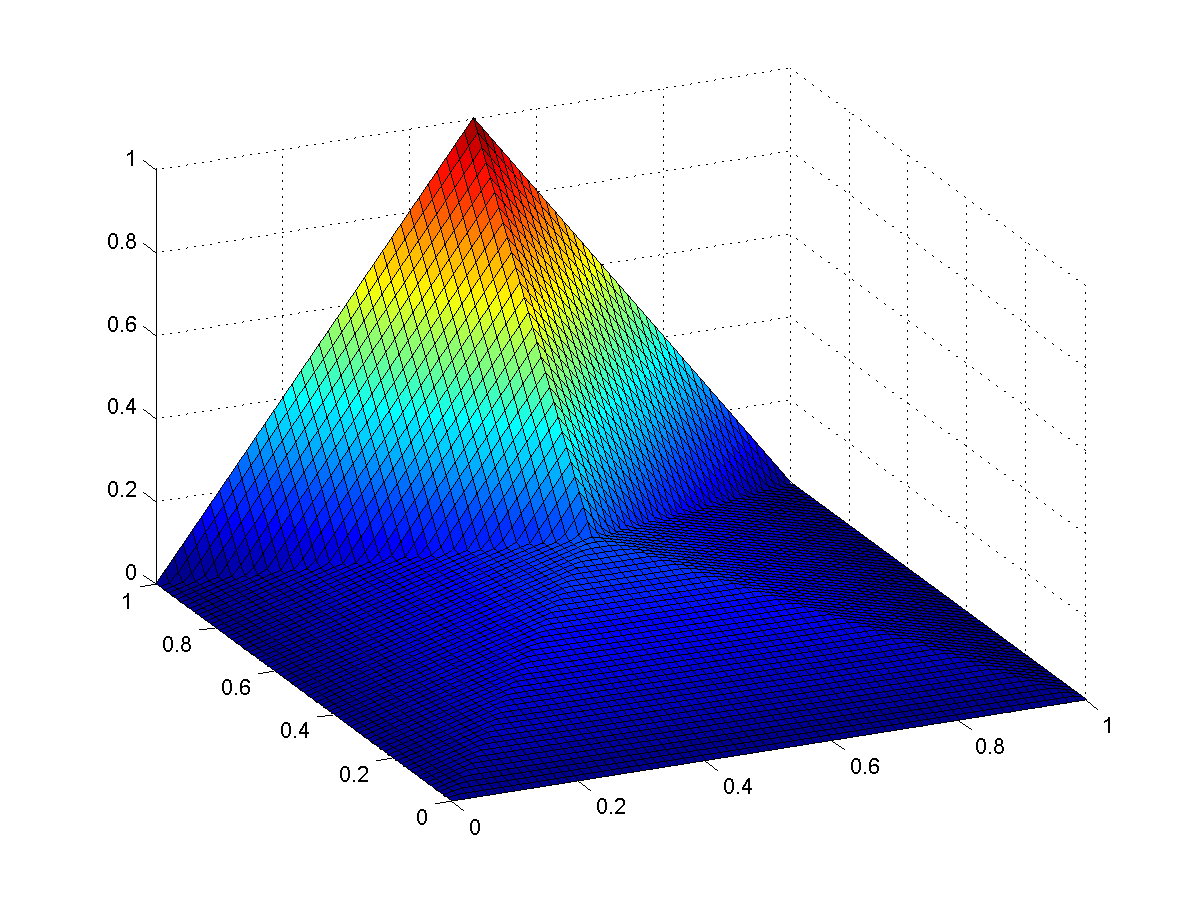
\includegraphics[width=\textwidth]{figures/sec_BF/PWL_dpent_plot_E.png}
		\caption{}
	\end{subfigure}
\caption{Plots of the PWL basis functions for a regular pentagon: (a) and (c) as well as a degenerate pentagon: (b) and (d).}
\end{figure}
% End::2D PWL basis function plots
%%%%%%%%%%%%%%%

%%%%%%%%%%%%%%%%%%%%%%%%%%%%%%%%%%%%%%%%%%%%%%%%%%%
%%%   SubSection - Mean Value
\subsection{Mean Value Basis Functions}
\label{sec::BF_2DLinear_MV}

At this point, we now introduce the first new polygonal basis set for use with the transport equation: the {\em mean value coordinates} (MV) developed by Floater \cite{floater2003mean,hormann2006mean}. The original motivation behind the MV coordinates was to approximate harmonic maps on a polygon by a set of piecewise linear maps over a triangulation of the polygon for use in computer aided graphic design. 

\begin{equation}
\label{eq::BF_MV_laplace}
\nabla^2 u = 0 ,
\end{equation}

\noindent with $u(\vec{r}) = u_0$ constituting a piecewise linear function 

\begin{equation}
\label{eq::BF_MV_BF}
b_{j}^{MV} (\vec{x}) = \frac{w_j (\vec{x}) }{\sum_i w_i (\vec{x})}
\end{equation}

\noindent where the mean value weight function for vertex $j$, $w_j$, has the following definition:

\begin{equation}
\label{eq::BF_MV_weights}
w_j (\vec{x})  = \frac{\tan(\alpha_{j-1} / 2) + \tan(\alpha_j / 2)}{|\vec{x}_j - \vec{x}|}
\end{equation}

%%%%%%%%%%%%%%%%%%%%%%%%%%%%%%%%%%%%%%%%%%%%%%%%%%%
%%%   SubSection - Maximum Entropy
\subsection{Maximum Entropy Basis Functions}
\label{sec::BF_2DLinear_ME}

The final linearly-complete 2D basis functions that we will analyze in this work are generated by use of the {\em maximum entropy coordinates} (ME) \cite{sukumar2004construction,hormann2008maximum}. 

\begin{equation}
\label{eq::BF_ME_BF}
b_{j}^{ME} (\vec{x}) = \frac{w_j (\vec{x}) }{\sum_i w_i (\vec{x})}
\end{equation}

\noindent where the maximum entropy weight function for vertex $j$, $w_j$, has the following definition:

\begin{equation}
\label{eq::BF_ME_weights}
w_j (\vec{x})  = m_j(\vec{x}) \exp(-  \kappa \cdot (\vec{x}_j - \vec{x}))
\end{equation}

\noindent In Eq. (\ref{eq::BF_ME_weights}), $m_j$ 

\begin{equation}
\label{eq::BF_ME_prior_funcs}
 m_j(\vec{x}) = \frac{\pi_j (\vec{x}) }{\sum_{k} \pi_k (\vec{x})}
\end{equation}

\noindent where

\begin{equation}
\label{eq::BF_ME_prior_products}
\pi_j (\vec{x}) = \prod\displaylimits_{i \neq j-1, j} \rho_j (\vec{x})
\end{equation}

\noindent where

\begin{equation}
\label{eq::BF_ME_face_funcs}
\rho_j (\vec{x}) = || \vec{x} - \vec{x}_j || + || \vec{x} - \vec{x}_{j+1} || - || \vec{x}_{j+1} - \vec{x}_j ||
\end{equation}

%%%%%%%%%%%%%%%%%%%%%%%%%%%%%%%%%%%%%%%%%%%%%%%%%%%
%%%   SubSection - 2D linear summary
\subsection{Summary of 2D Linear Basis Functions on Polygons}
\label{sec::BF_2DLinear_Summary}



%%%%%%%%%%%%%%%%%%%%%%%%%%%%%%%%%%%%%%%%%%%%%%%%%%%
%%%   Section - Quadratic Basis Functions
\section{Quadratic Serendipity Basis Functions on 2D Polygons}
\label{sec::BF_2DQuadratic}

%%%%%%%%%%%%%%%%%%%%%%%%%%%%%%%%%%%%%%%%%%%%%%%%%%%
%%%   SubSection - P2 and S2
\subsection{Traditional Quadratic Basis Functions - $\mathbb{P}_{2}$ and $\mathbb{S}_{2}$ Spaces}
\label{sec::BF_2DQuadratic_P2S2}


%%%%%%%%%%%%%%%%%%%%%%%%%%%%%%%%%%%%%%%%%%%%%%%%%%%
%%%   SubSection - Quadratice ME
\subsection{Quadratic Mean Value Coordinates on 2D Polygons}
\label{sec::BF_2DQuadratic_ME}


%%%%%%%%%%%%%%%%%%%%%%%%%%%%%%%%%%%%%%%%%%%%%%%%%%%
%%%   SubSection - Quadratice ME
\subsection{Quadratic Maximum Entropy Coordinates on 2D Polygons}
\label{sec::BF_2DQuadratic_ME}



%%%%%%%%%%%%%%%%%%%%%%%%%%%%%%%%%%%%%%%%%%%%%%%%%%%
%%%   Section - 3D
\section{Linear Basis Functions on 3D Polyhedra}
\label{sec::BF_3DLinear}



%%%%%%%%%%%%%%%%%%%%%%%%%%%%%%%%%%%%%%%%%%%%%%%%%%%
%%%   SubSection - 3D Lin/TriL
\subsection{3D Linear and TriLinear Basis Functions}
\label{sec::BF_3DLinear_TriL}

\begin{figure}
\centering
	\begin{subfigure}[b]{0.45\textwidth}
		\centering
		\label{subfig::unit_square}
		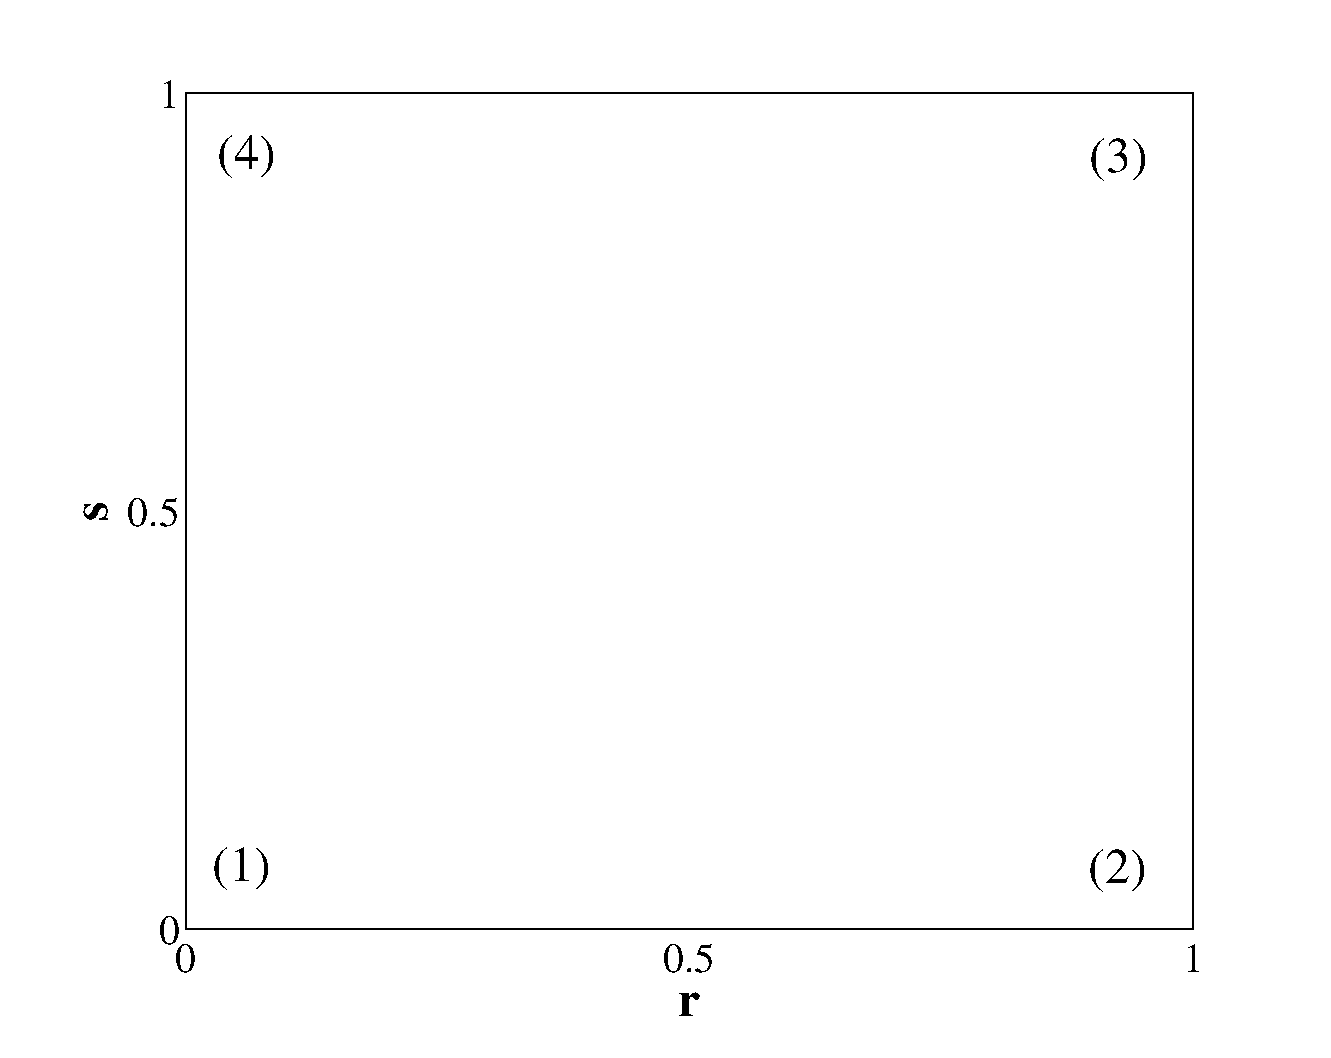
\includegraphics[width=\textwidth]{figures/sec_BF/unit_square_linear.eps}
		\caption{}
	\end{subfigure}
	\hfill
	\begin{subfigure}[b]{0.45\textwidth}
		\centering
		\label{subfig::unit_cube}
		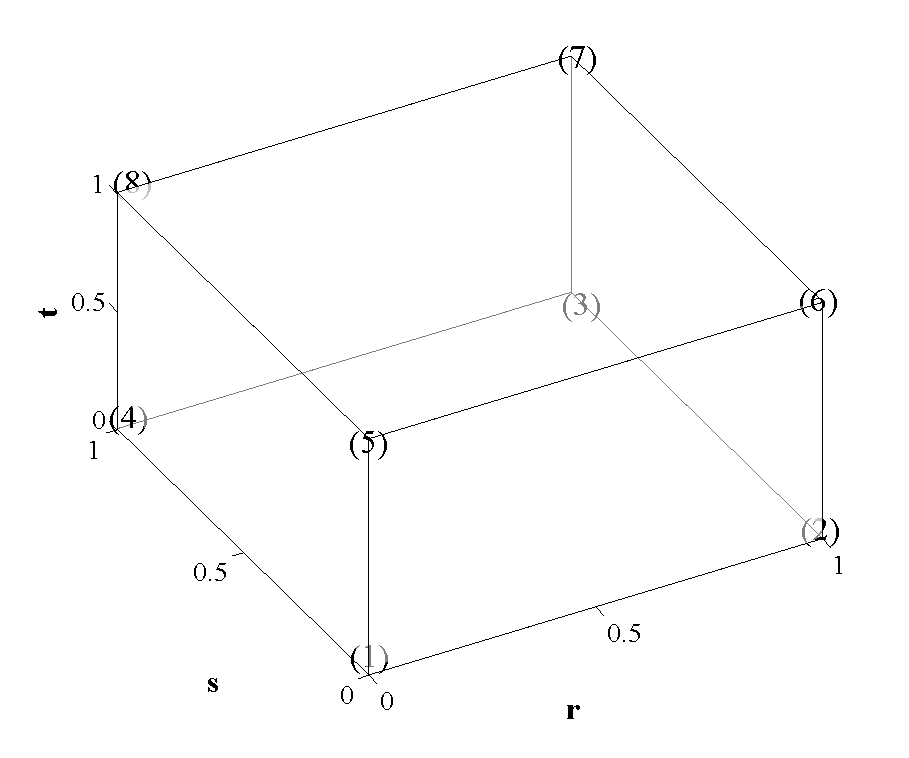
\includegraphics[width=\textwidth]{figures/sec_BF/unit_cube_linear.eps}
		\caption{}
	\end{subfigure}
\caption{Vertex structure for the (a) unit square and (b) unit cube.}
\label{fig::BF_3D_unit_tet_cube}
\end{figure}

\begin{equation}
\label{eq::3D_lin_basis_functions}
\begin{aligned}
	b_1(r,s) & = 1-r-s-t \\
	b_2(r,s) & = r \\
	b_3(r,s) & = s \\
	b_4(r,s) & = t
\end{aligned}
\end{equation}

\noindent and

\begin{equation}
\label{eq::TriL_basis_functions}
\begin{aligned}
	b_1(r,s,t) & = (1-r)(1-s)(1-t) \\
	b_2(r,s,t) & = r(1-s)(1-t) \\
	b_3(r,s,t) & = rs(1-t) \\
	b_4(r,s,t) & = (1-r)s(1-t) \\
	b_5(r,s,t) & = (1-r)(1-s)t \\
	b_6(r,s,t) & = r(1-s)t \\
	b_7(r,s,t) & = rst \\
	b_8(r,s,t) & = (1-r)st \\
\end{aligned}
\end{equation}

%%%%%%%%%%%%%%%%%%%%%%%%%%%%%%%%%%%%%%%%%%%%%%%%%%%
%%%   SubSection - PWL
\subsection{3D Piecewise Linear (PWL) Basis Functions}
\label{sec::BF_3DLinear_PWL}

The 3D PWL basis functions share a similar form to the 2D PWL basis functions.

\begin{equation}
\label{eq::PWL_3D}
	b_j (x,y,z)  = t_j  (x,y,z) + \sum_{f=1}^{F_j} \beta_f^j  t_f (x,y,z) + \alpha_j^K t_c  (x,y,z)
\end{equation}

\noindent $t_j$ is the standard 3D linear function with unity at vertex $j$ that linearly decreases to zero to the cell center, the face center for each face that includes vertex $j$, and each vertex that shares an edge with vertex $j$. $t_c$ is the 3D cell ``tent" function which is unity at the cell center and linearly decreases to zero to each cell vertex and face center. $t_f$ is the face "tent" function which is unity at the face center and linearly decreases to zero at each vertex on that face and the cell center. $\beta_{f,j}$ is the weight parameter for face $f$ touching cell vertex $j$, and $F_j$ is the number of faces touching vertex $j$. Like the previous work defining the PWLD method \cite{bailey2008phd}, we also choose to assume the cell and face weighting parameters are

\begin{equation}
\alpha_{K,j} = \frac{1}{N_K} \qquad \text{and} \qquad \beta_{f,j} = \frac{1}{N_f},
\label{eq::PWL_weight_vals}
\end{equation}

\noindent respectively, where $N_K$ is the number of vertices in cell $K$ and $N_f$ is the number of vertices on face $f$, which leads to constant values of $\alpha$ and $\beta$ for each cell and face, respectively. This assumption of the cell weight function holds for both 2D and 3D.

%%%%%%%%%%%%%%%%%%%%%%%%%%%%%%%%%%%%%%%%%%%%%%%%%%%
%%%   Section - Results
\section{Numerical Results}
\label{sec::BF_Results}

Now that we have presented several linear polygonal finite element basis sets along with the methodology to convert them to quadratic serendipity-like basis, we present several numerical problems to demonstrate our methodology. First, we demonstrate that the presented basis sets can capture an exactly-linear transport solution in Section \ref{sec::BF_Results_Linear}. Next, we present some convergence properties of the basis sets using the method of manufactured solutions (MMS) in Section \ref{sec::BF_Results_MMS}. We then present a searchlight problem and observe how the basis sets react with adaptive mesh refinement (AMR) to mitigate numerical dispersion through a vacuum in Section \ref{sec::BF_Results_SL}.

%%%%%%%%%%%%%%%%%%%%%%%%%%%%%%%%%%%%%%%%%%%%%%%%%%%
%%%   SubSection - Linear Solutions = METHOD OF EXACT SOLUTIONS
\subsection{Two-Dimensional Exactly-Linear Transport Solutions}
\label{sec::BF_Results_Linear}

We present our first numerical example by demonstrating that the linear and quadratic polygonal finite element basis functions capture an exactly-linear solution space. We will show this by the method of exact solutions (MES). Since the coordinate interpolation of the basis functions for the linear basis functions requires exact linear interpolation (Eq. (\ref{eq::BF_linear_interp_affine})), then an exactly-linear solution space can be captured, even on highly distorted polygonal meshes. This also applies to the quadratic serendipity space since it is formed by the product-wise pairings of the linear basis functions. We build our exact solution by investigating the 2D, 1 energy group transport problem with no scattering and an angle-dependent distributed source,

\begin{equation}
\label{eq::BF_Results_Linear_angflux}
\mu \frac{\partial \Psi}{\partial x} + \eta \frac{\partial \Psi}{\partial y} + \sigma_t \Psi = Q(x,y, \mu, \eta), 
\end{equation}

\noindent where the streaming term was separated into the corresponding two-dimensional terms. We chose to drop the scattering term for this example so that the error arising from iteratively converging our solution would have no impact.

We then define an angular flux solution that is linear in both space and angle along with the corresponding 0th moment scalar flux ($\Phi_{0,0} \rightarrow \Phi$) solution:

\begin{equation}
\label{eq::BF_Results_Linear_fluxsols}
\begin{aligned}
\Psi (x,y,\mu,\eta) &= ax + by + c \mu + d\eta + e\\
\Phi (x,y) &= 2 \pi \left( ax + by  + e \right)
\end{aligned} .
\end{equation}

\noindent One can immediately notice that our 0th moment solution is not dependent on angle. We arrive at this solution by enforcing our 2D angular quadrature set to have the following properties:

\begin{equation}
\label{eq::BF_Results_Linear_quadrules}
\sum_{q} w_q = 2 \pi \qquad \text{and} \qquad \sum_{q} w_q  \left[
	\begin{array}{c}
		\mu_q \\
		\eta_q
	\end{array} \right] = \left[
	\begin{array}{c}
		0 \\
		0
	\end{array} \right] .
\end{equation}

Our boundary conditions for all inflow boundaries are then uniquely determined by the angular flux solution of Eq. (\ref{eq::BF_Results_Linear_fluxsols}). Inserting the angular flux solution of Eq. (\ref{eq::BF_Results_Linear_fluxsols}) into Eq. (\ref{eq::BF_Results_Linear_angflux}), we obtain the distributed source that will produce our exactly-linear solution space:

\begin{equation}
\label{eq::BF_Results_Linear_src}
Q(x,y,\mu,\eta) = a \mu + b \eta + \sigma_t \left(  c \mu + d \eta \right) + \sigma_t \left( ax +by + e   \right).
\end{equation}

\noindent It is noted that the angular dependence of the source can be removed (which can ease the code development burden) if one sets

\begin{equation}
\label{eq::BF_Results_Linear_removeterms}
\begin{aligned}
	a &= - c \, \sigma_t, \\
	b &= - d \, \sigma_t.
\end{aligned}
\end{equation}

For this example, we test the various 2D polygonal finite element basis functions on six different mesh types. These mesh types include triangular, quadrilateral, and polygonal meshes:

\begin{enumerate}
	\item Orthogonal cartesian mesh formed by the intersection of 11 equally-spaced vertices in both the $x$ and $y$ dimensions. This forms a 10x10 array of quadrilateral mesh cells.
	\item Ordered-triangular mesh formed by the bisection of the previous orthogonal cartesian mesh (forming 200 triangles all of the same size/shape).
	\item Quadrilateral shestakov grid formed by the randomization of vertices based on a skewness parameter \cite{shestakov1988solution,shestakov1990test}. With a certain range of this skewness parameter, highly distorted meshes can be generated.
	\item Sinusoidal polygonal grid that is generated by the transformation of a uniform orthogonal grid based on a sinusoid functional. The transformed vertices are then converted into a polygonal grid by computing a bounded Voronoi diagram.
	\item Kershaw's quadrilateral z-mesh \cite{kershaw1981differencing}. This mesh is formed by taking an orthogonal quadrilateral grid and displacing certain interior vertices only in the $y$ dimension.
	\item A polygonal variant of the quadrilateral z-mesh. The polygonal grid is formed in a similar manner to the sinusoidal polygonal mesh with a Voronoi diagram.
\end{enumerate}

\noindent We also wish that both the angular flux solution as well as the 0th moment solution are strictly positive everywhere. Therefore, we set the function parameters in Eq. (\ref{eq::BF_Results_Linear_fluxsols}) to $\sigma_t = a = c = d = e = 1.0$ and $b = 1.5$. We gave the solution the $40 \%$ tilt in space ($a \neq b$) so that it would not align with the triangular mesh. Using an S8 LS quadrature set, we ran all combinations of the polygonal basis functions and the mesh types. The linear solutions for the Wachspress, PWL, mean value, linear maximum entropy, and quadratic serendipity maximum entropy basis functions are presented in Figures \ref{fig::BF_Results_Linear_wach_sol}, \ref{fig::BF_Results_Linear_pwld_sol}, \ref{fig::BF_Results_Linear_mv_sol}, \ref{fig::BF_Results_Linear_me1_sol}, and \ref{fig::BF_Results_Linear_me2_sol}, respectively. We can see that for all the polygonal basis functions, an exact linear solution is captured as shown by the unbroken nature of the contour lines. This even holds on the highly distorted quadrilateral shestakov mesh.

%%%%%%%%%%%%%%%%%
% Begin Linear Solution figures
\begin{figure}
\centering
	\begin{subfigure}[b]{0.45\textwidth}
		\centering
		\label{subfig::cart_wach_lin_sol}
		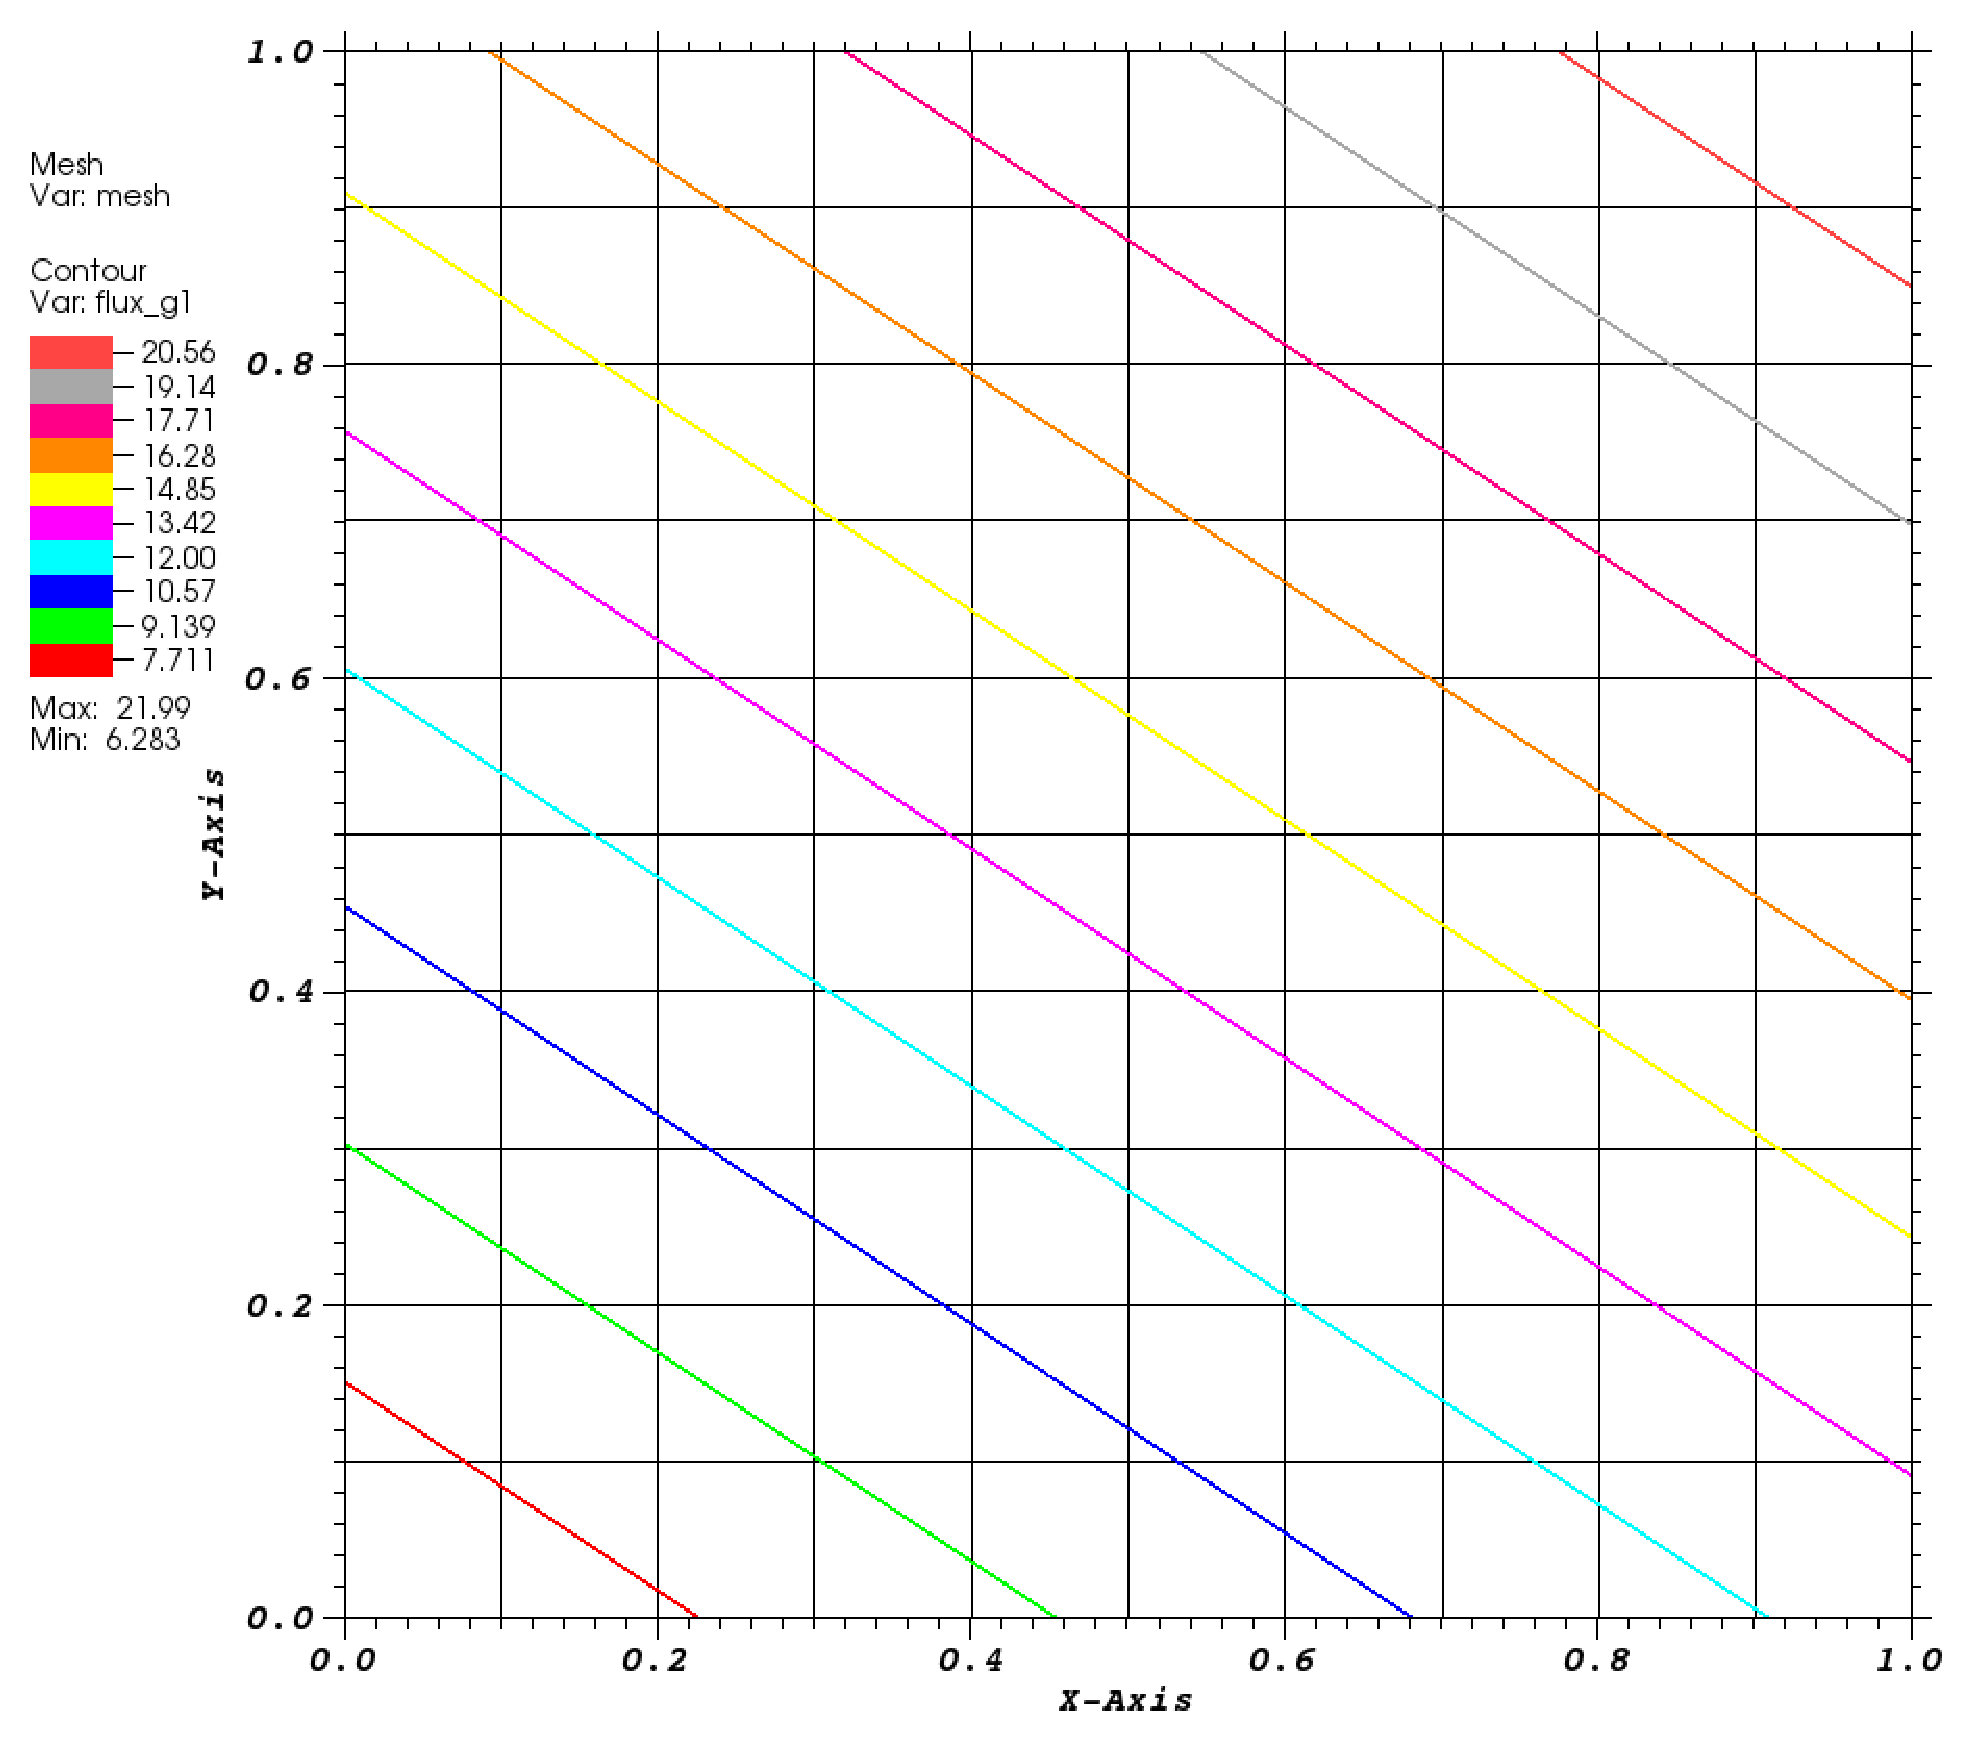
\includegraphics[width=\textwidth]{figures/sec_BF/cart_WACHSPRESS_k1.eps}
		\caption{}
	\end{subfigure}
	\hfill
	\begin{subfigure}[b]{0.45\textwidth}
		\centering
		\label{subfig::tri_wach_lin_sol}
		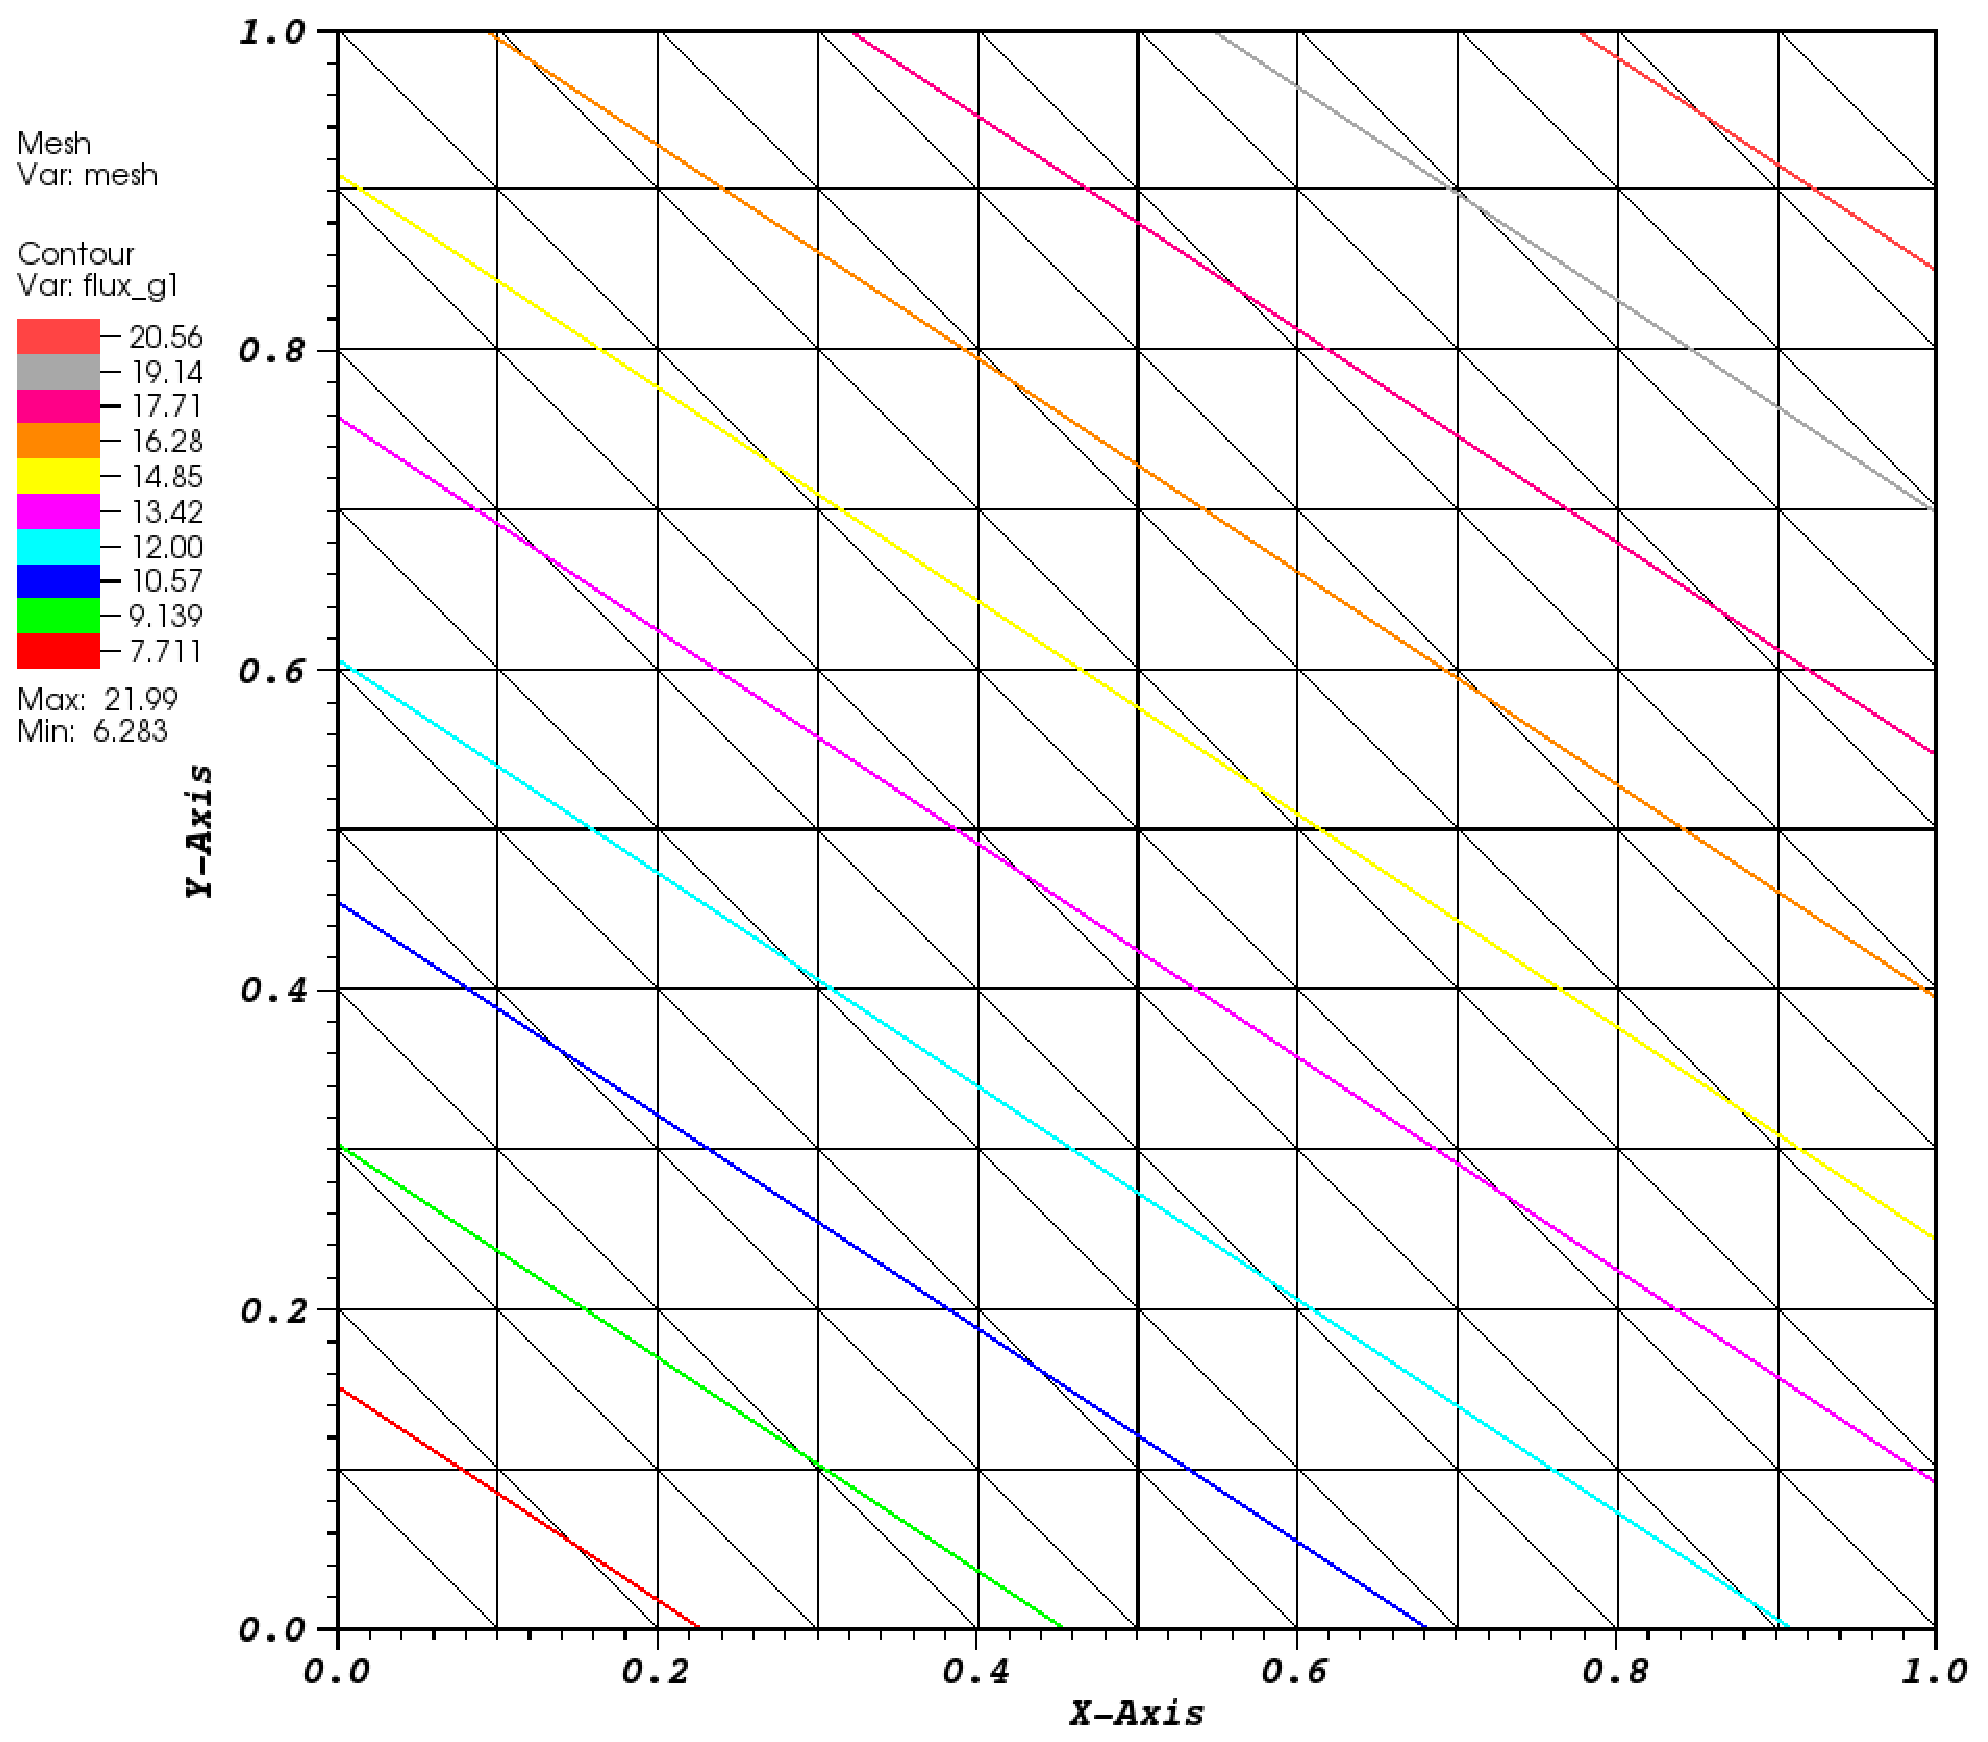
\includegraphics[width=\textwidth]{figures/sec_BF/tri_WACHSPRESS_k1.eps}
		\caption{}
	\end{subfigure}
	\vfill
	\begin{subfigure}[b]{0.45\textwidth}
		\centering
		\label{subfig::shes_quad_wach_lin_sol}
		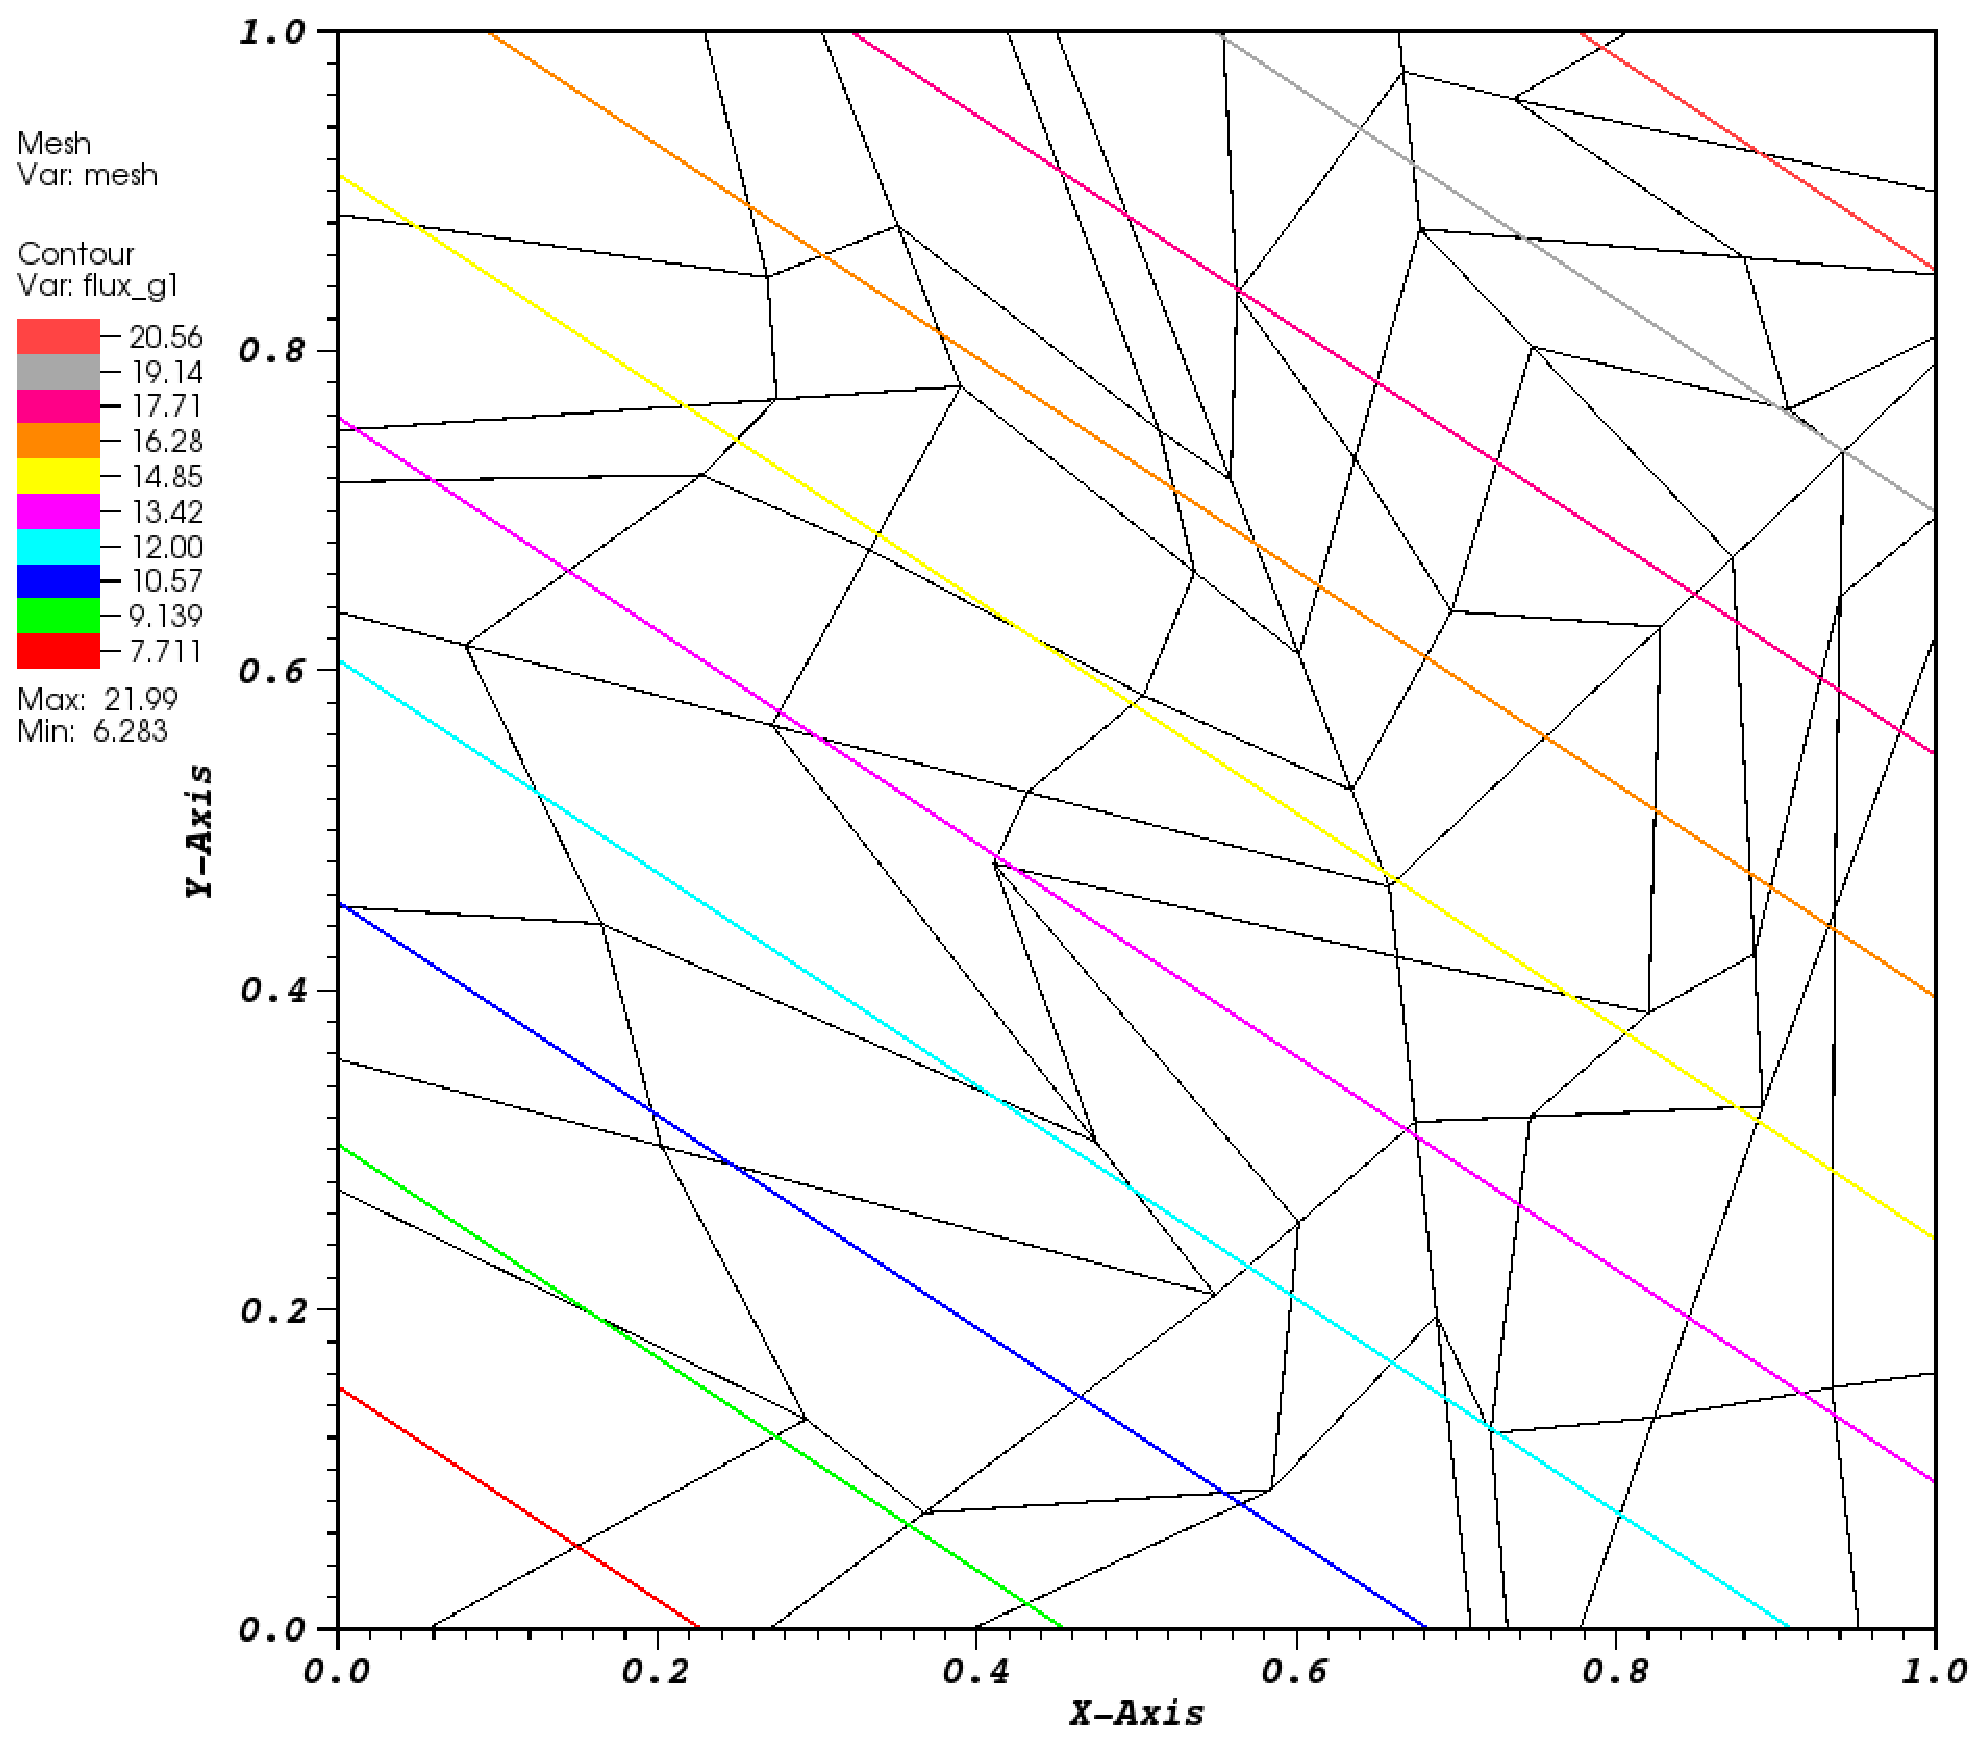
\includegraphics[width=\textwidth]{figures/sec_BF/shes_quad_WACHSPRESS_k1.eps}
		\caption{}
	\end{subfigure}
	\hfill
	\begin{subfigure}[b]{0.45\textwidth}
		\centering
		\label{subfig::smooth_poly_wach_lin_sol}
		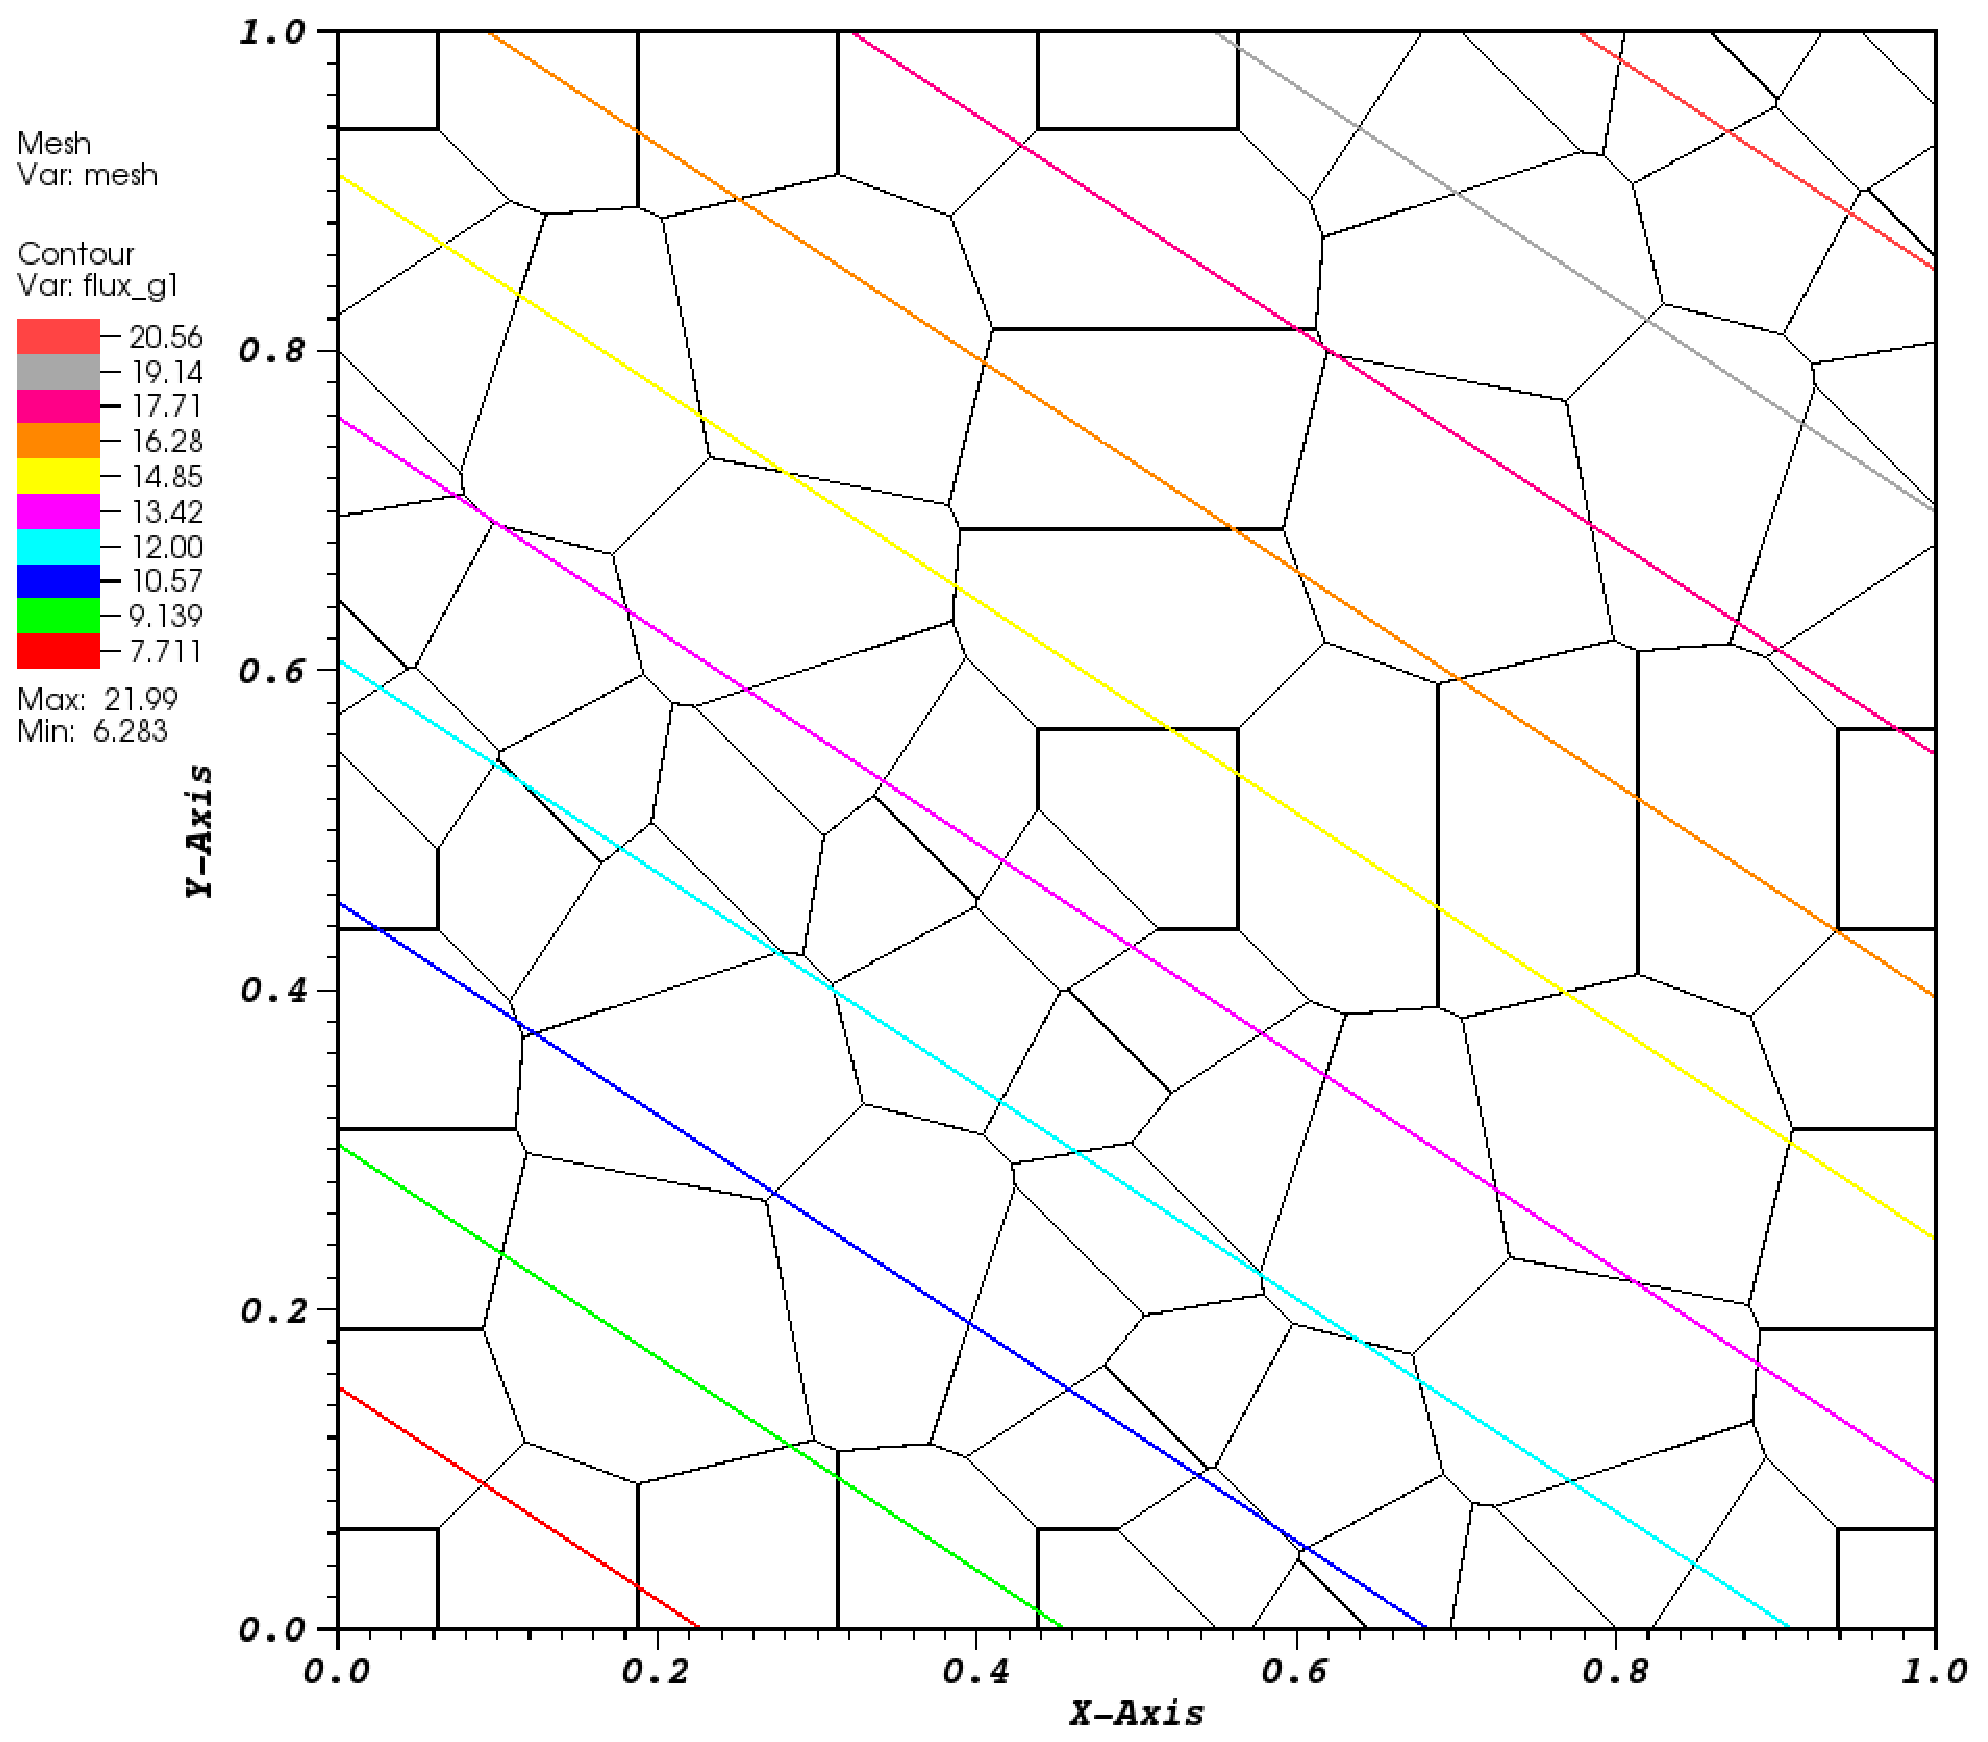
\includegraphics[width=\textwidth]{figures/sec_BF/smooth_poly_WACHSPRESS_k1.eps}
		\caption{}
	\end{subfigure}
	\vfill
	\begin{subfigure}[b]{0.45\textwidth}
		\centering
		\label{subfig::z_quad_wach_lin_sol}
		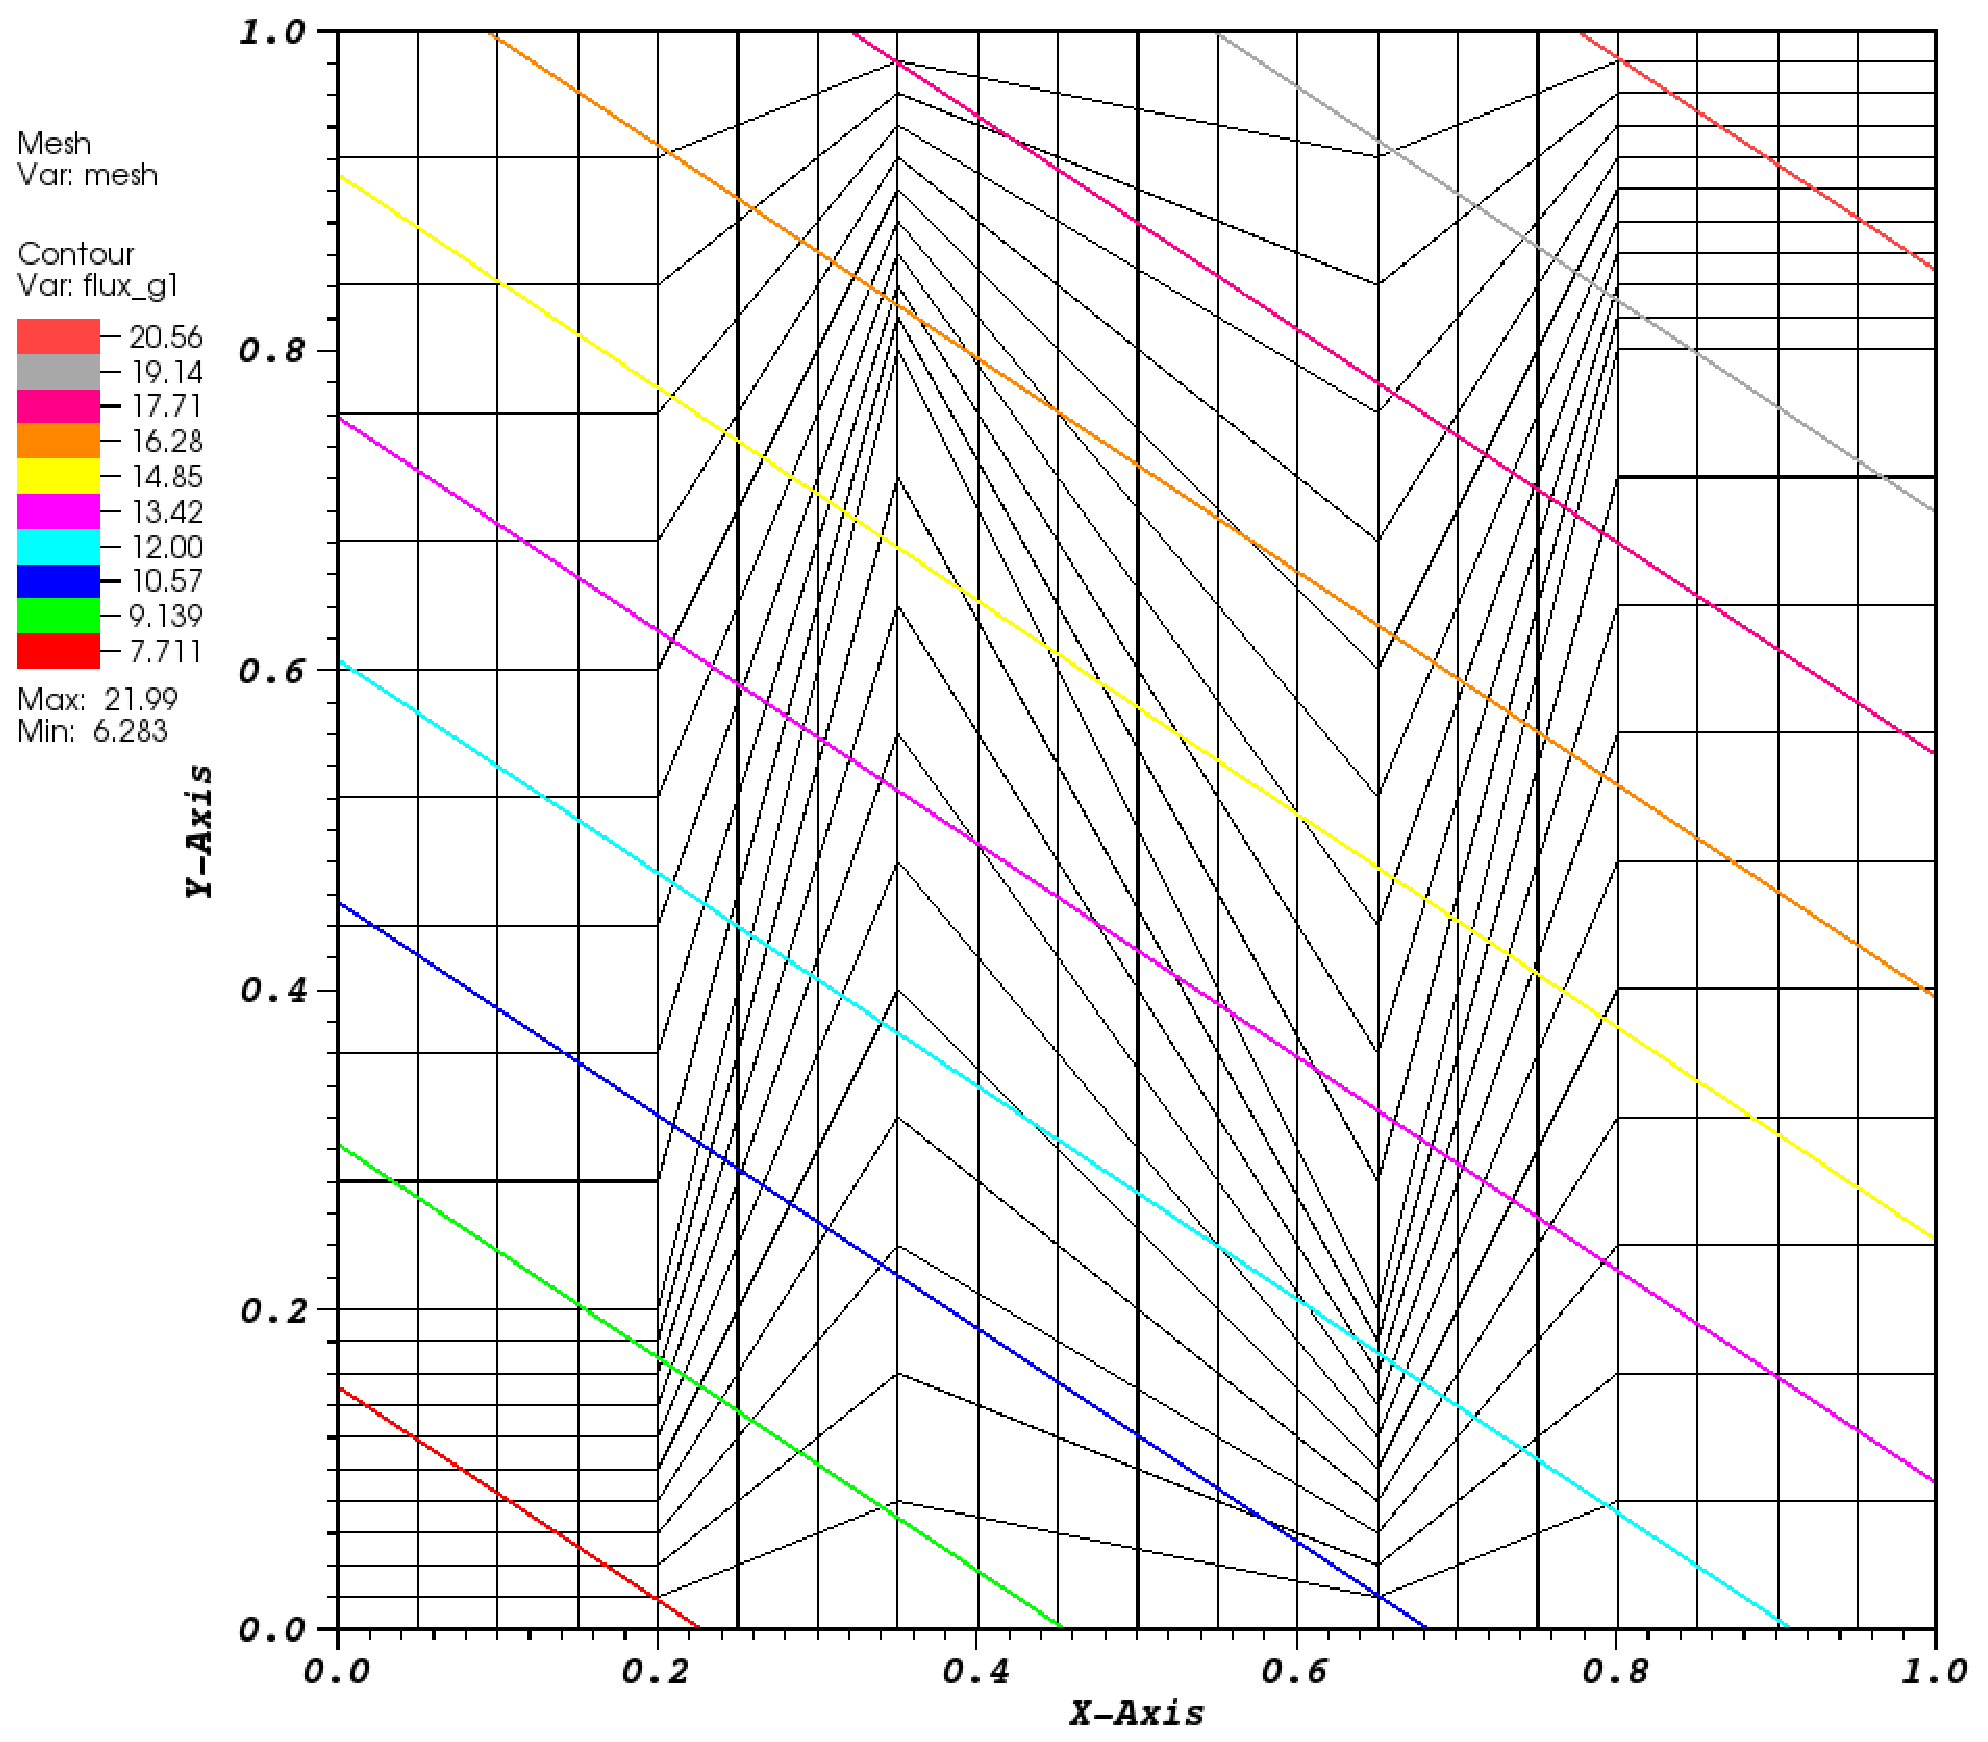
\includegraphics[width=\textwidth]{figures/sec_BF/z_quad_WACHSPRESS_k1.eps}
		\caption{}
	\end{subfigure}
	\hfill
	\begin{subfigure}[b]{0.45\textwidth}
		\centering
		\label{subfig::z_poly_wach_lin_sol}
		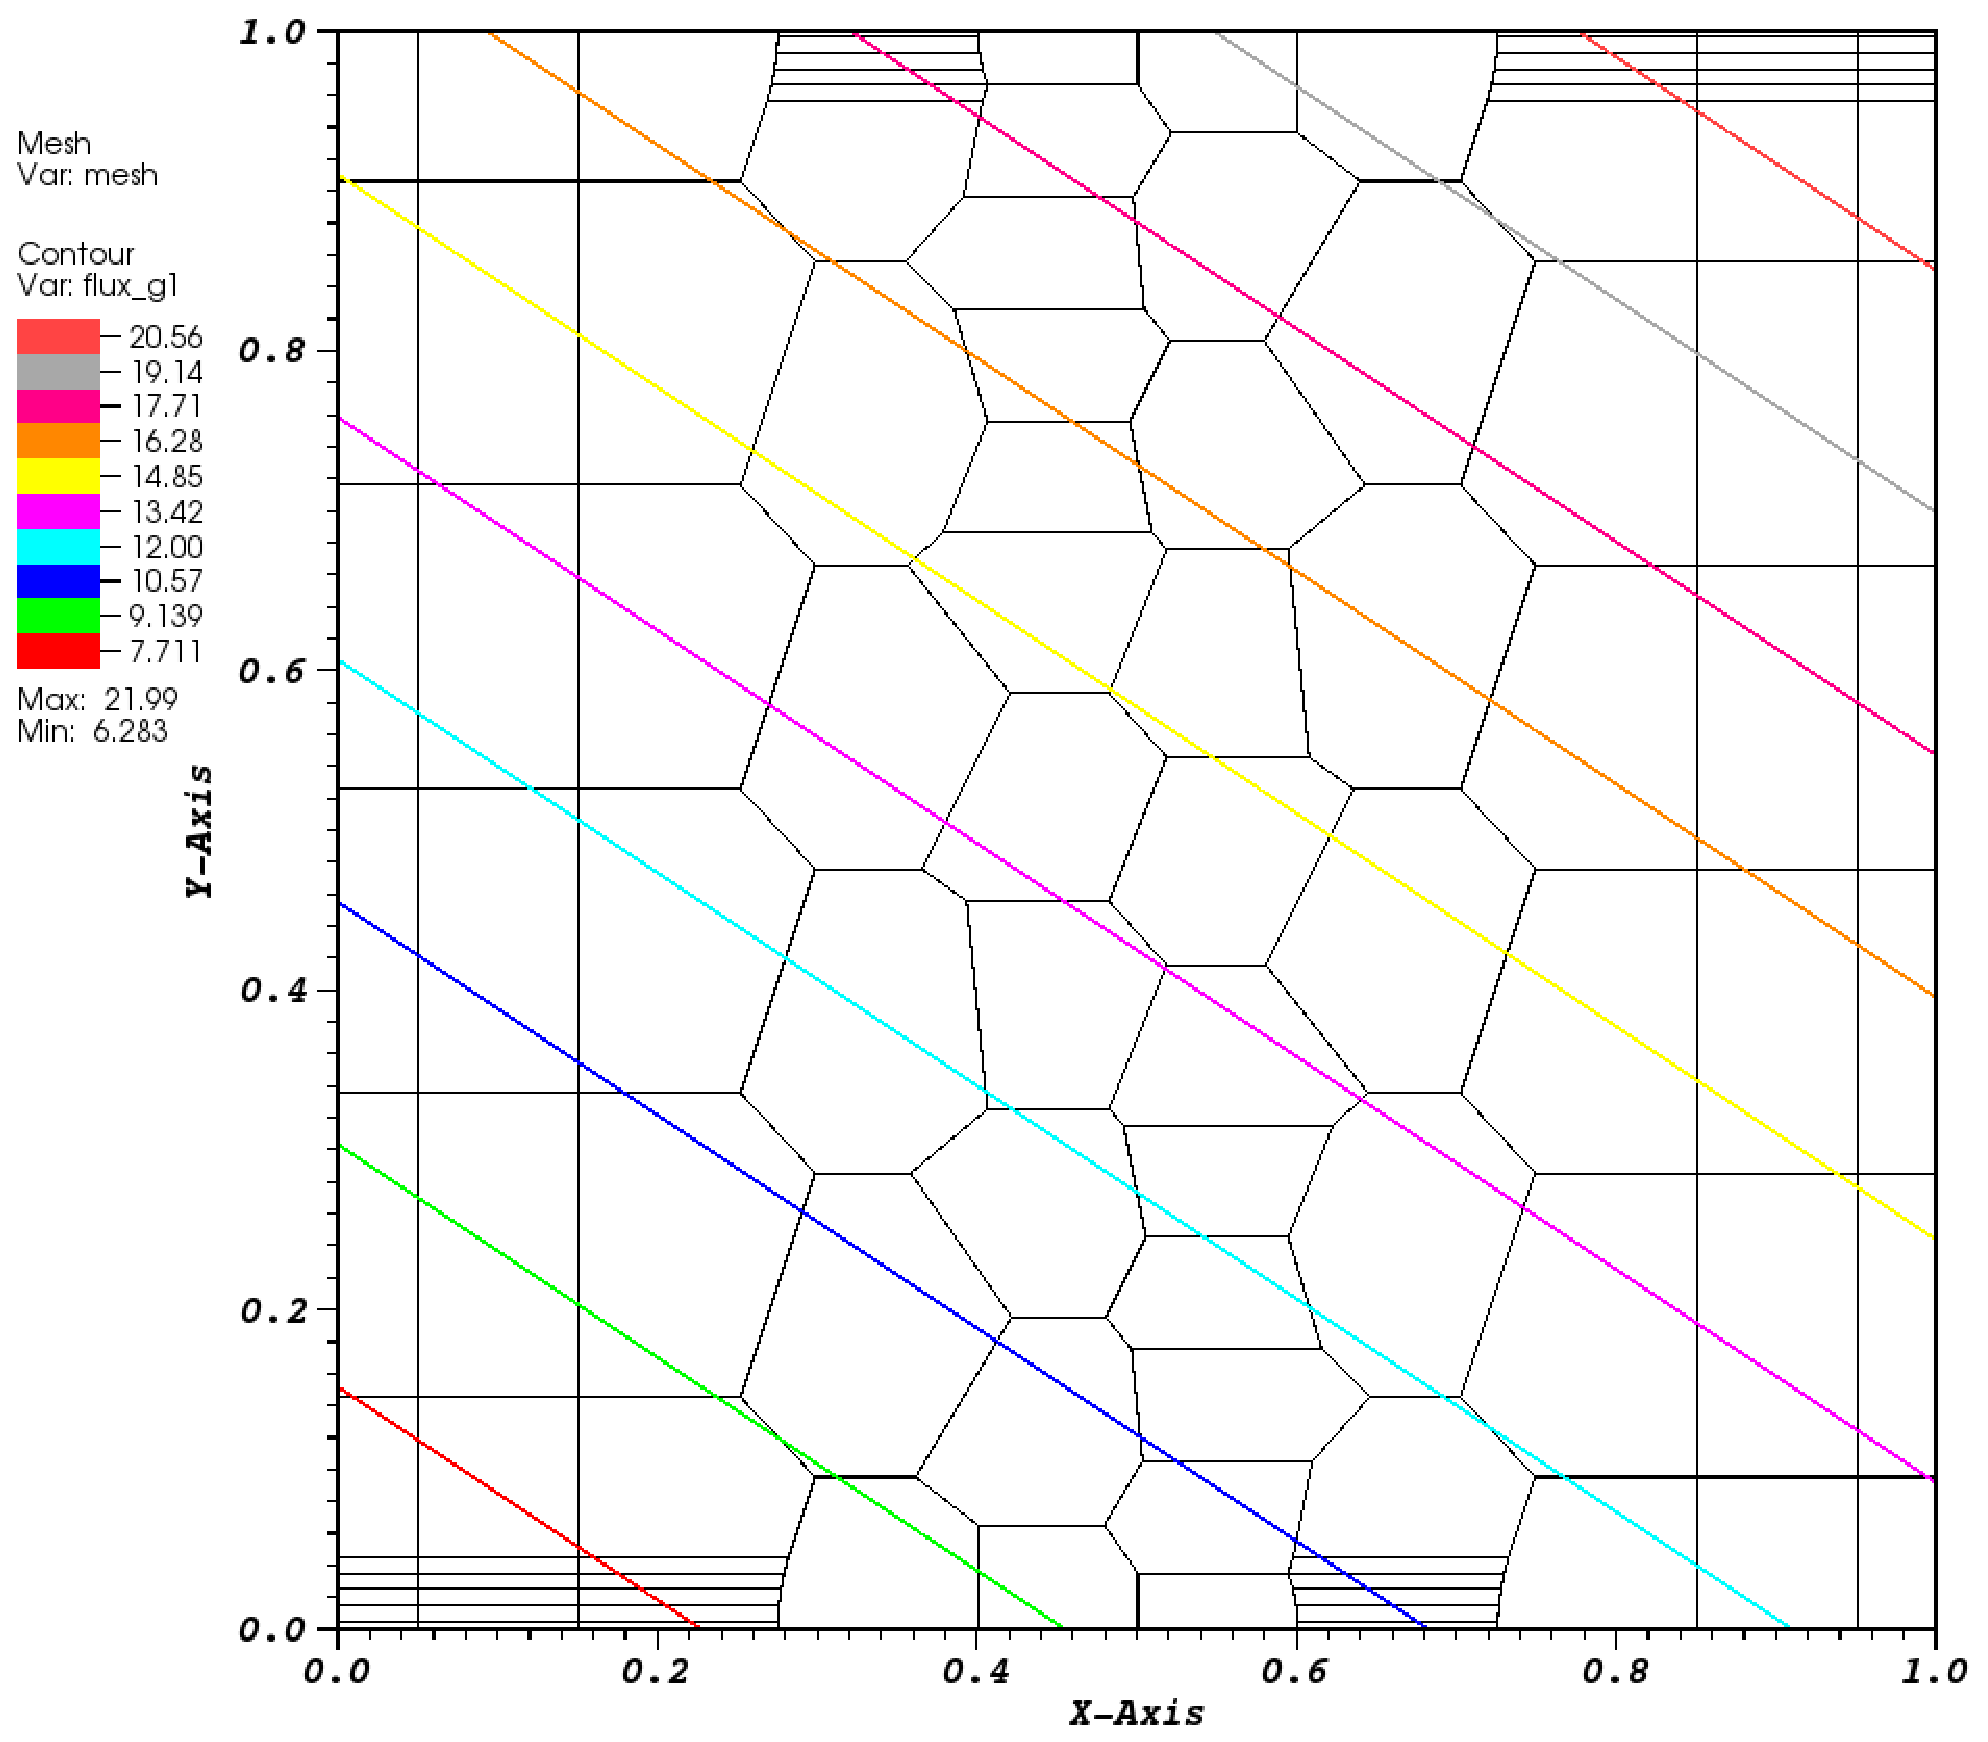
\includegraphics[width=\textwidth]{figures/sec_BF/z_poly_WACHSPRESS_k1.eps}
		\caption{}
	\end{subfigure}
\caption{Contour plots of the exactly-linear solution with the Wachspress basis functions on (a) cartesian mesh, (b) ordered-triangular mesh, (c) quadrilateral shestakov mesh, (d) sinusoidal polygonal mesh, (e) quadrilateral z-mesh, and (f) polygonal z-mesh.}
\label{fig::BF_Results_Linear_wach_sol}
\end{figure}

\begin{figure}
\centering
	\begin{subfigure}[b]{0.45\textwidth}
		\centering
		\label{subfig::cart_pwld_lin_sol}
		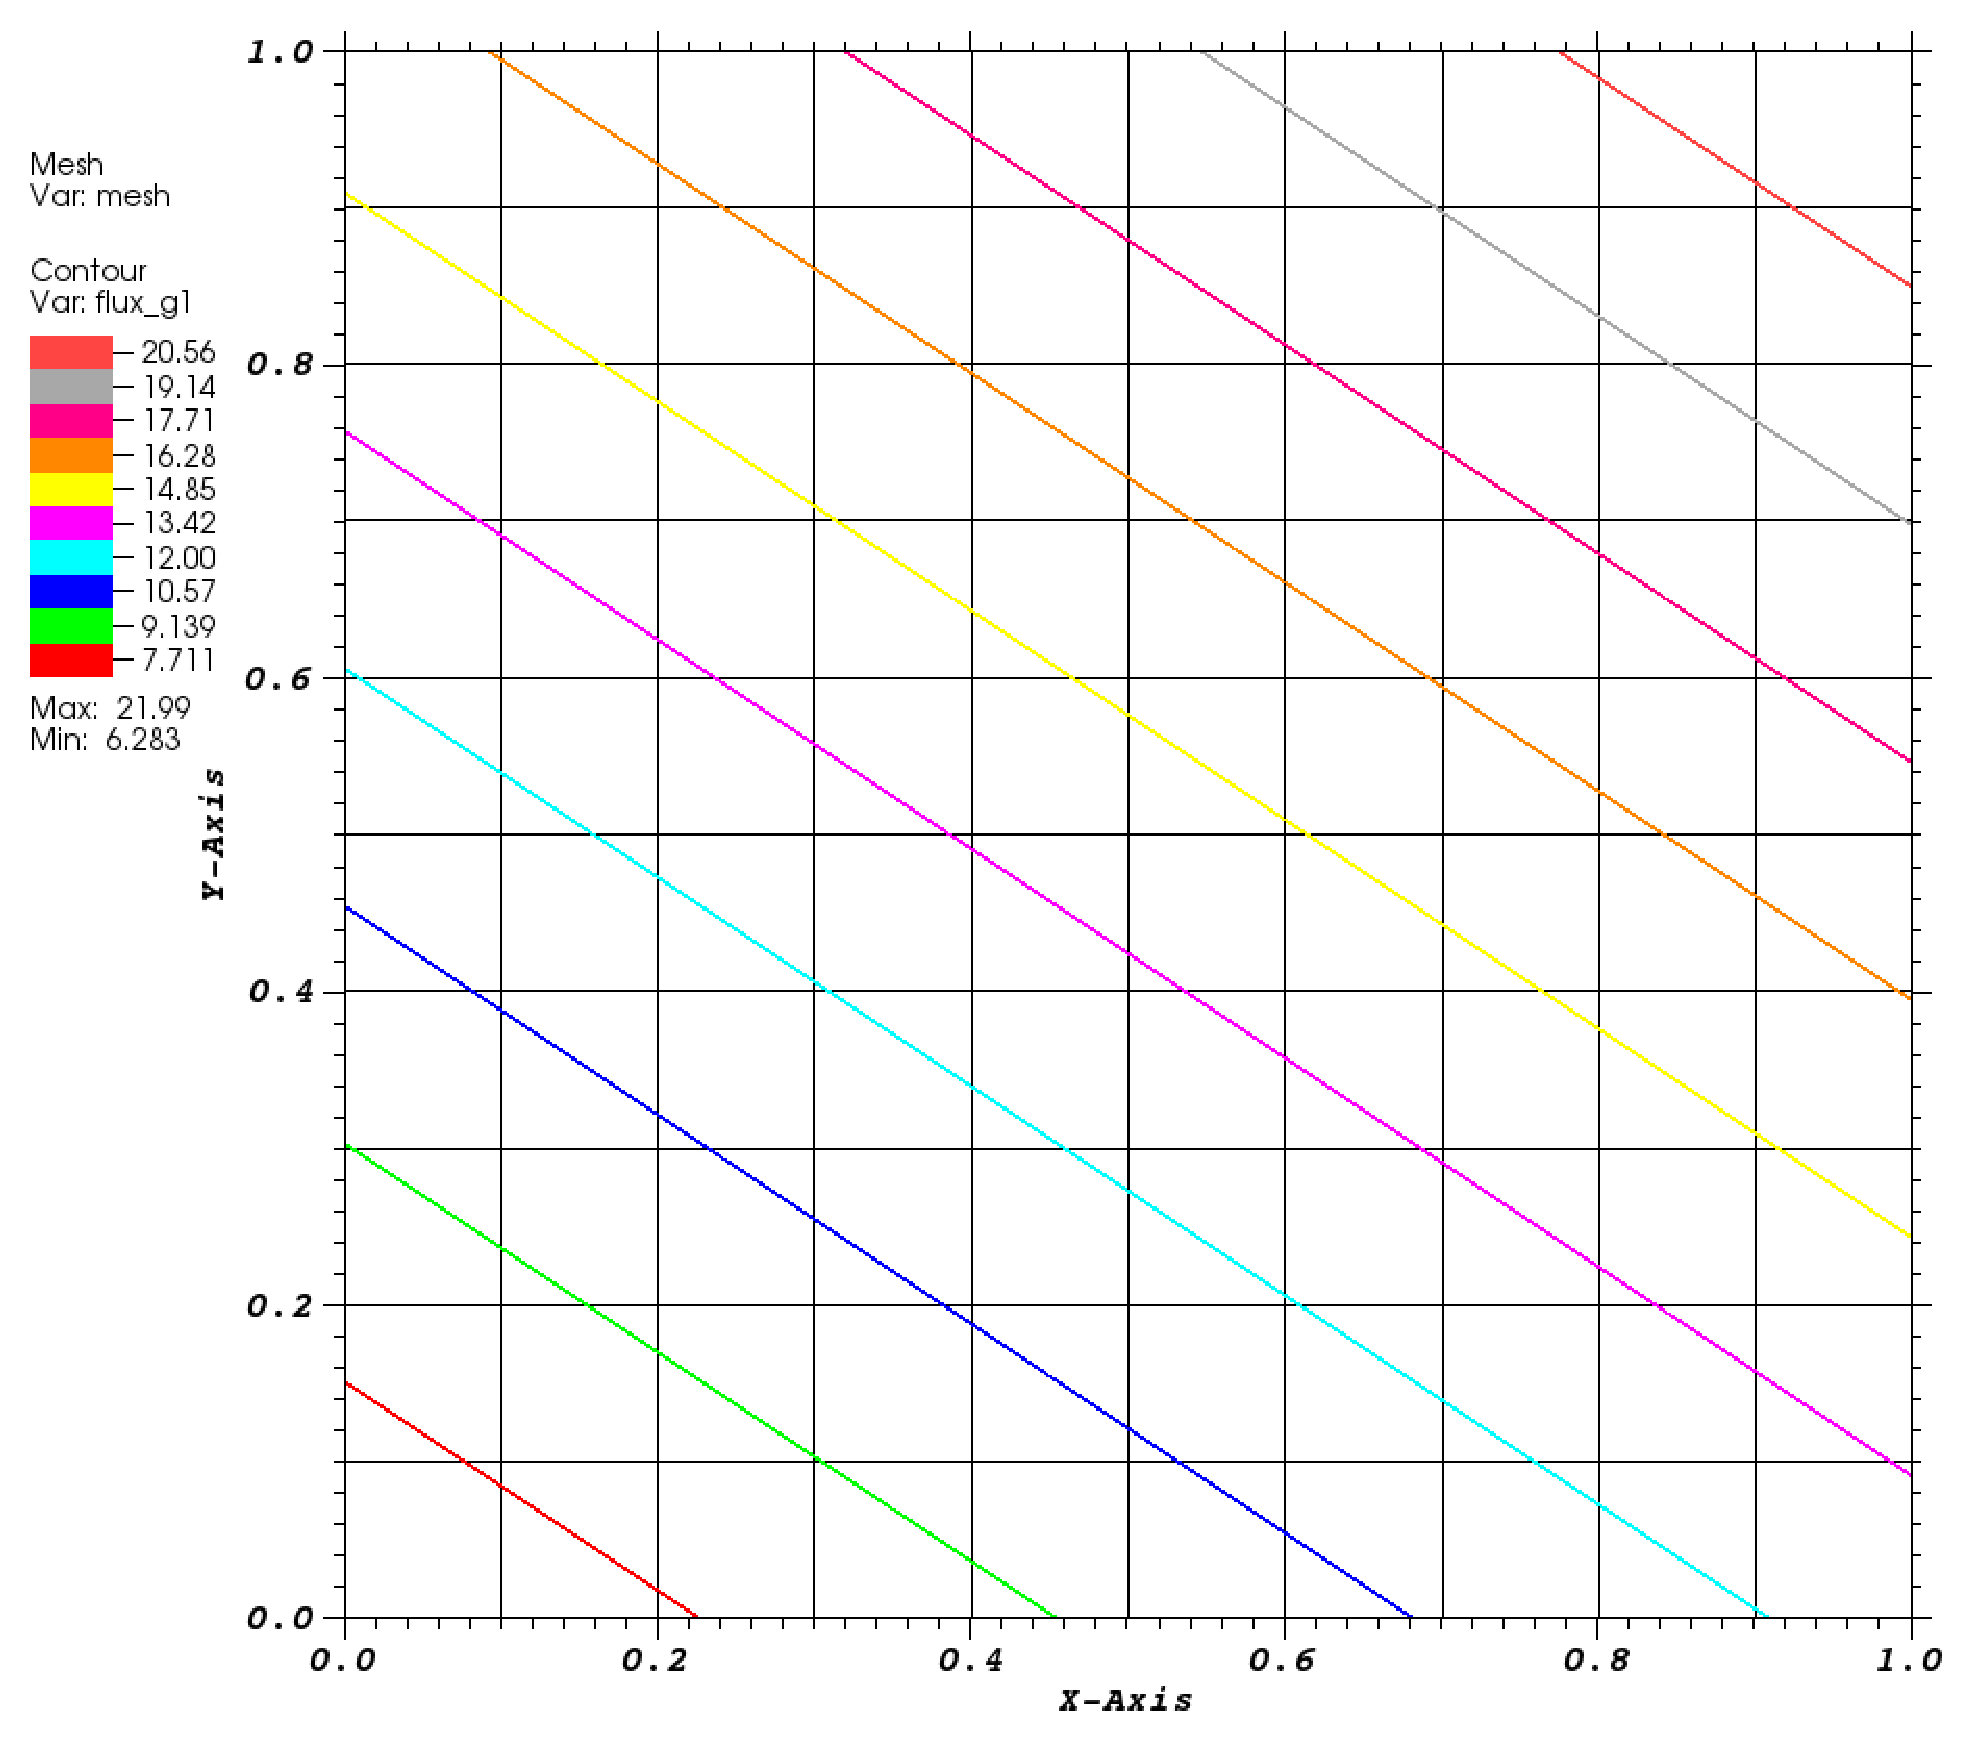
\includegraphics[width=\textwidth]{figures/sec_BF/cart_PWLD_k1.eps}
		\caption{}
	\end{subfigure}
	\hfill
	\begin{subfigure}[b]{0.45\textwidth}
		\centering
		\label{subfig::tri_pwld_lin_sol}
		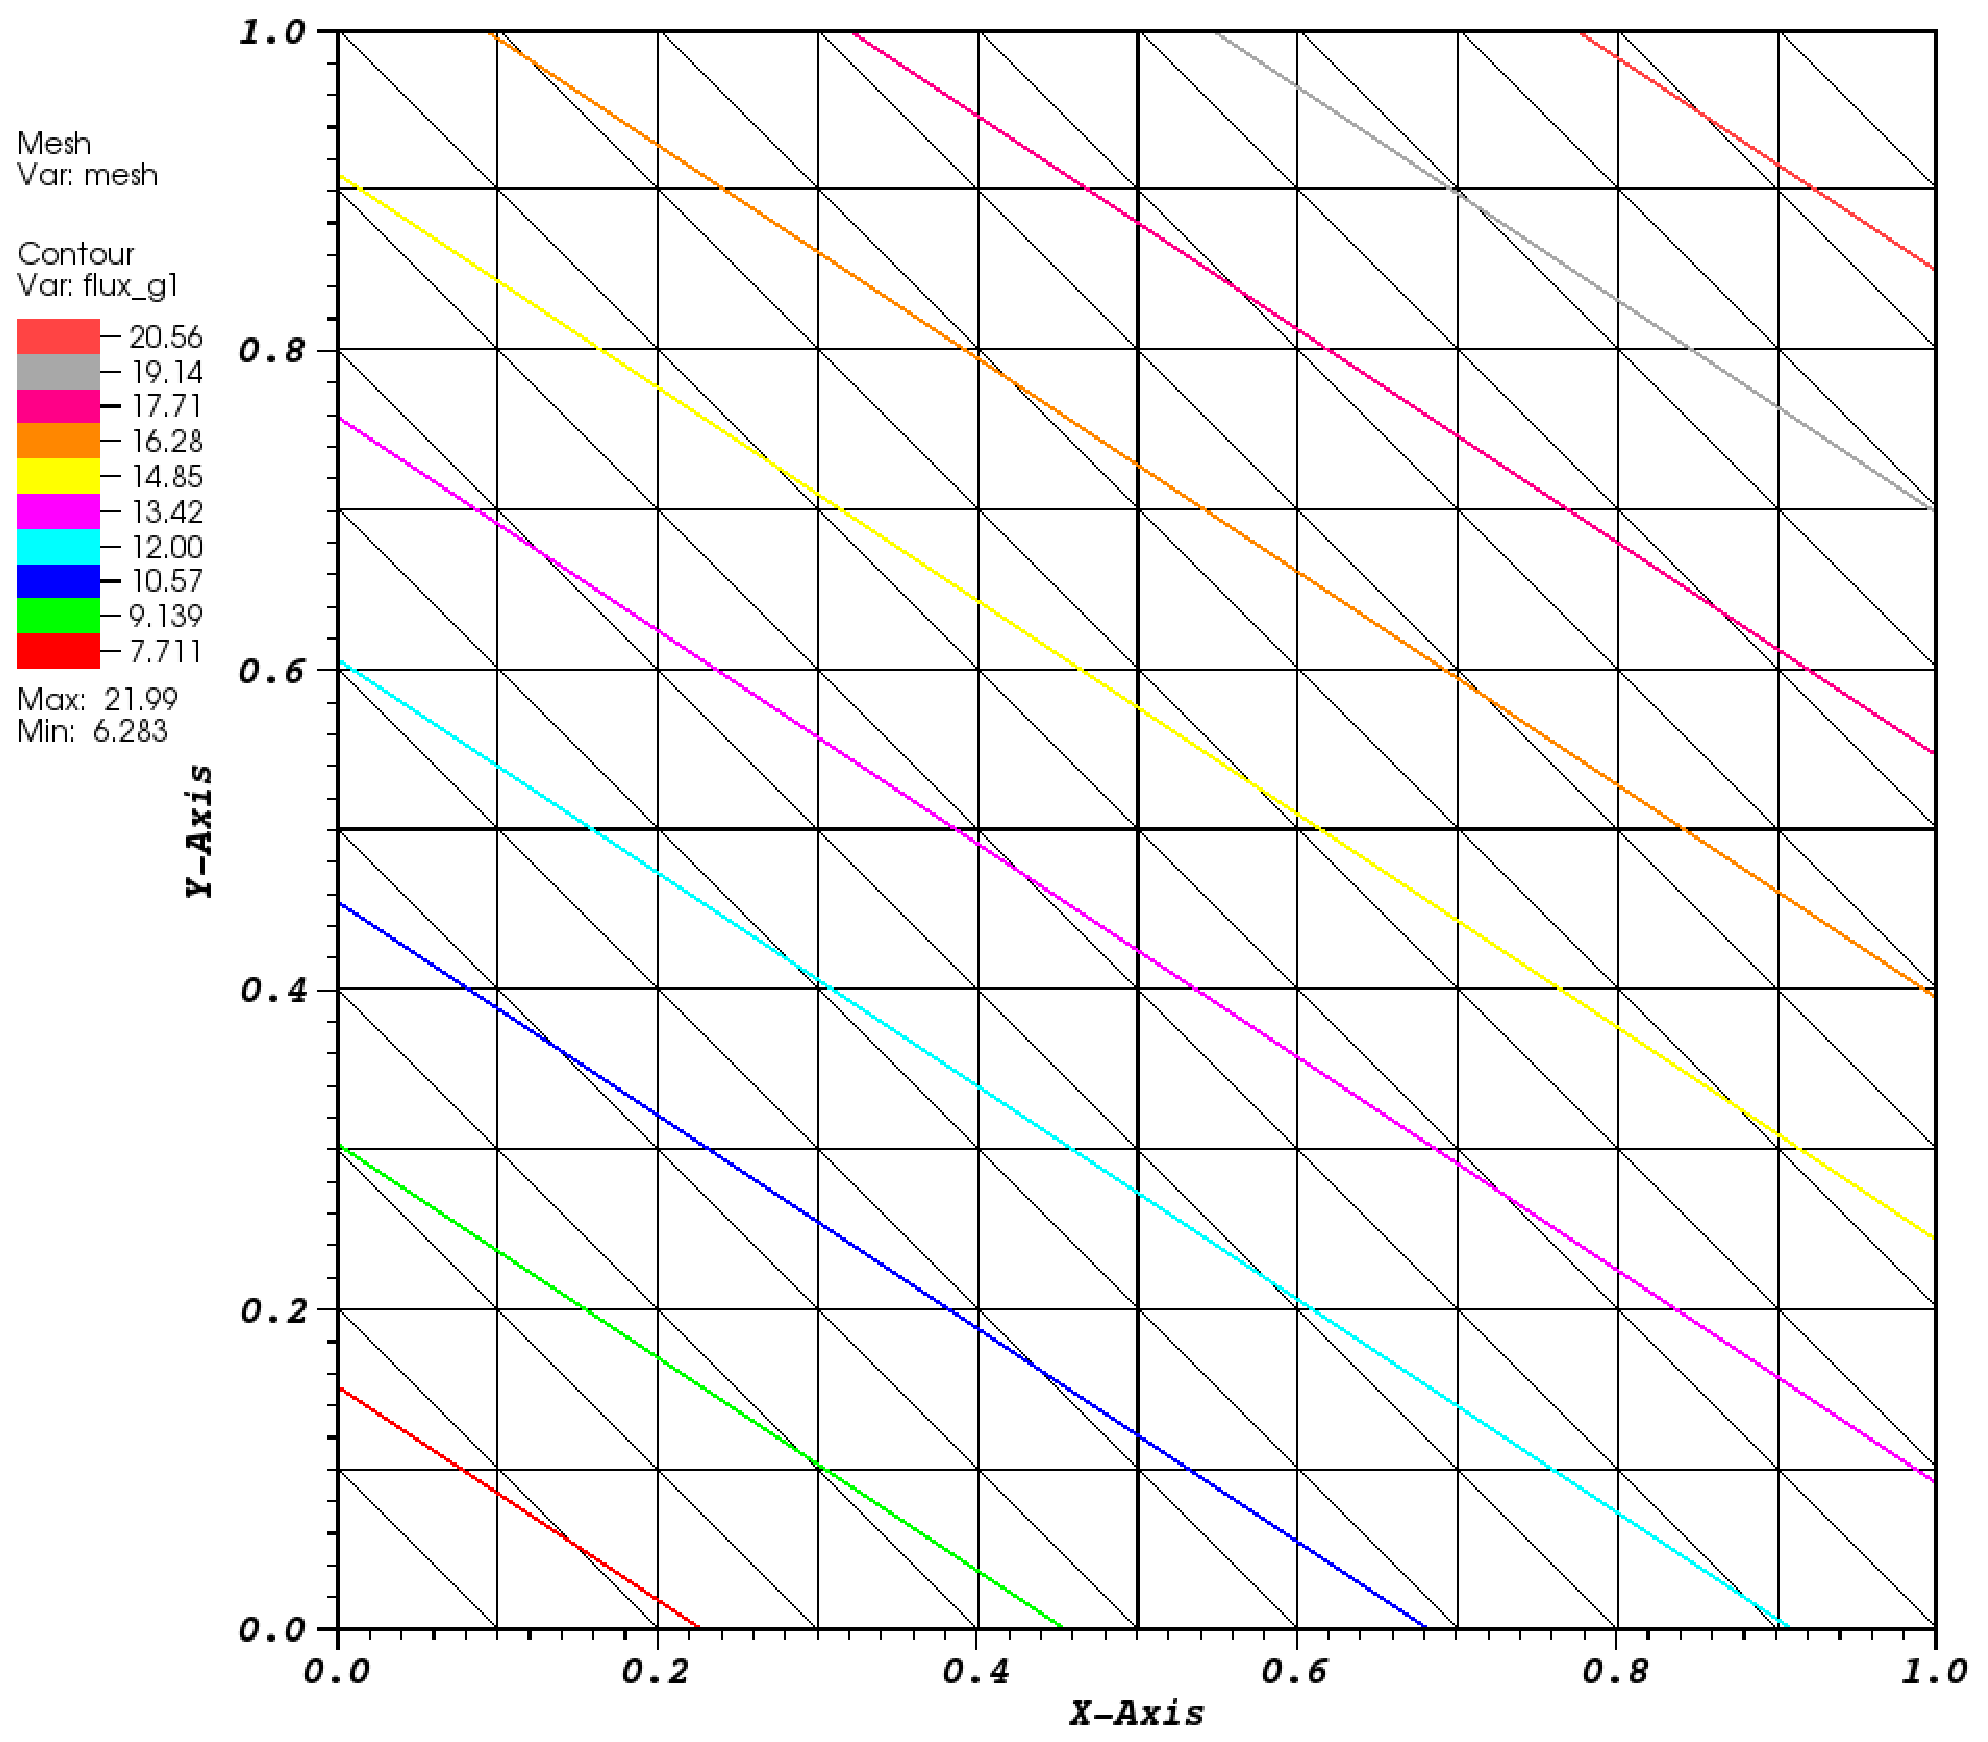
\includegraphics[width=\textwidth]{figures/sec_BF/tri_PWLD_k1.eps}
		\caption{}
	\end{subfigure}
	\vfill
	\begin{subfigure}[b]{0.45\textwidth}
		\centering
		\label{subfig::shes_quad_pwld_lin_sol}
		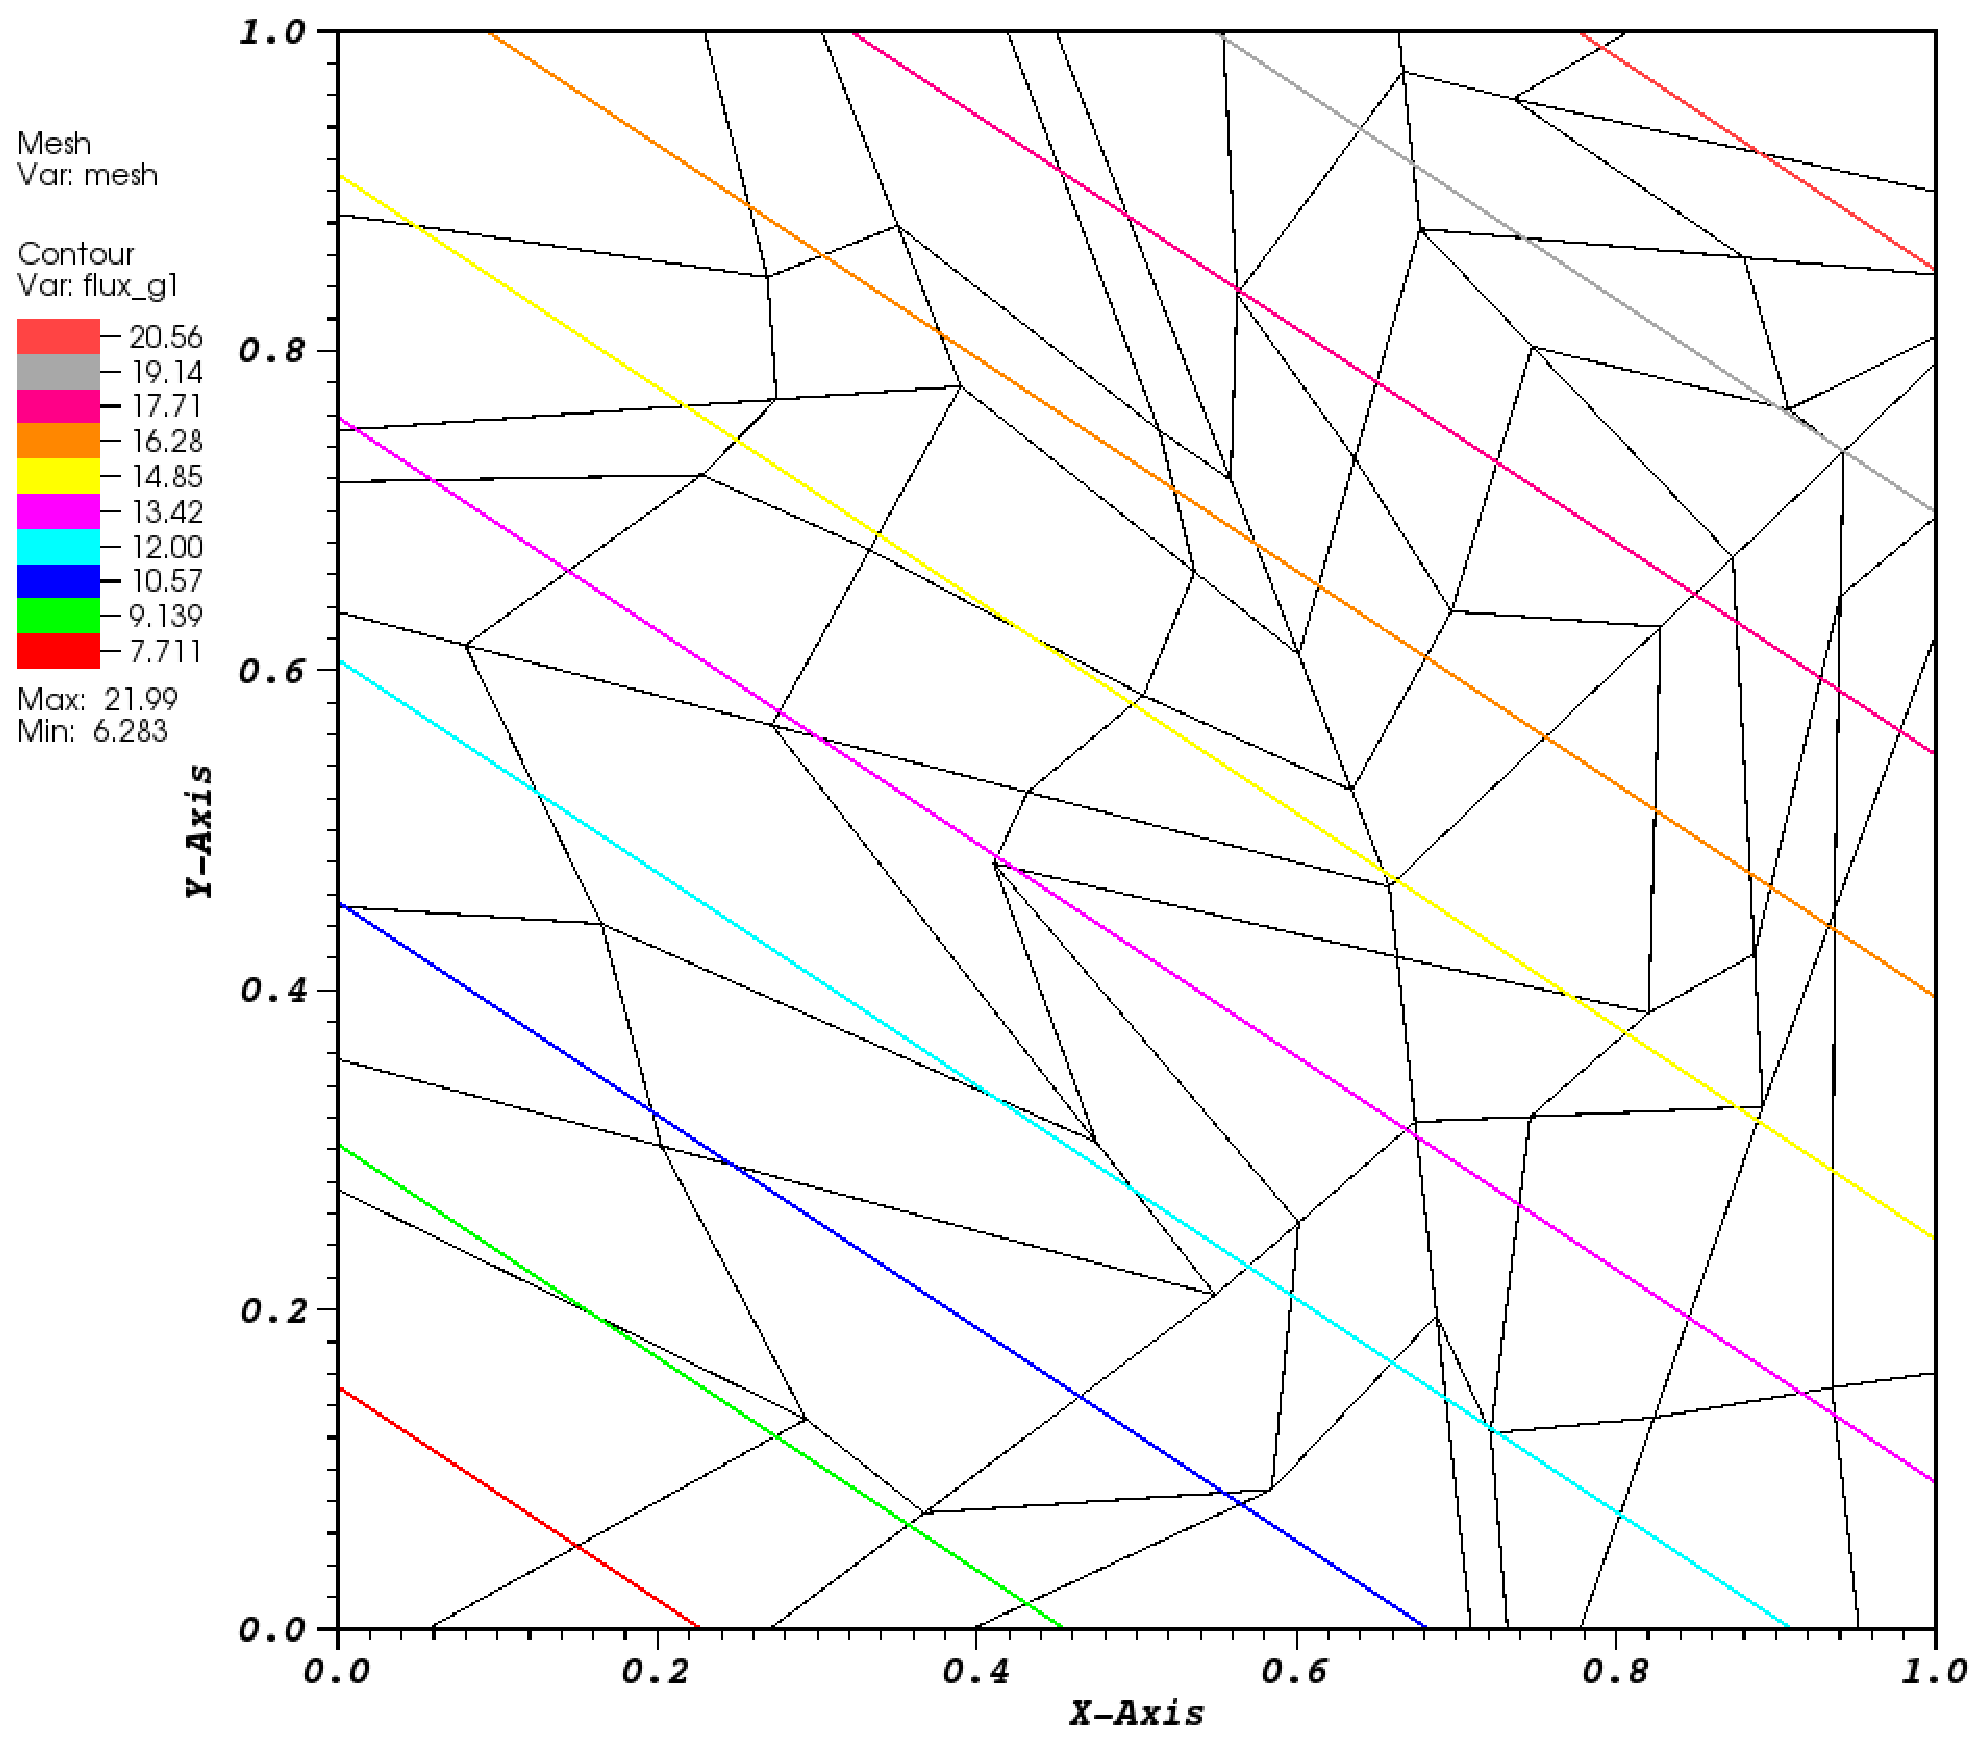
\includegraphics[width=\textwidth]{figures/sec_BF/shes_quad_PWLD_k1.eps}
		\caption{}
	\end{subfigure}
	\hfill
	\begin{subfigure}[b]{0.45\textwidth}
		\centering
		\label{subfig::smooth_poly_pwld_lin_sol}
		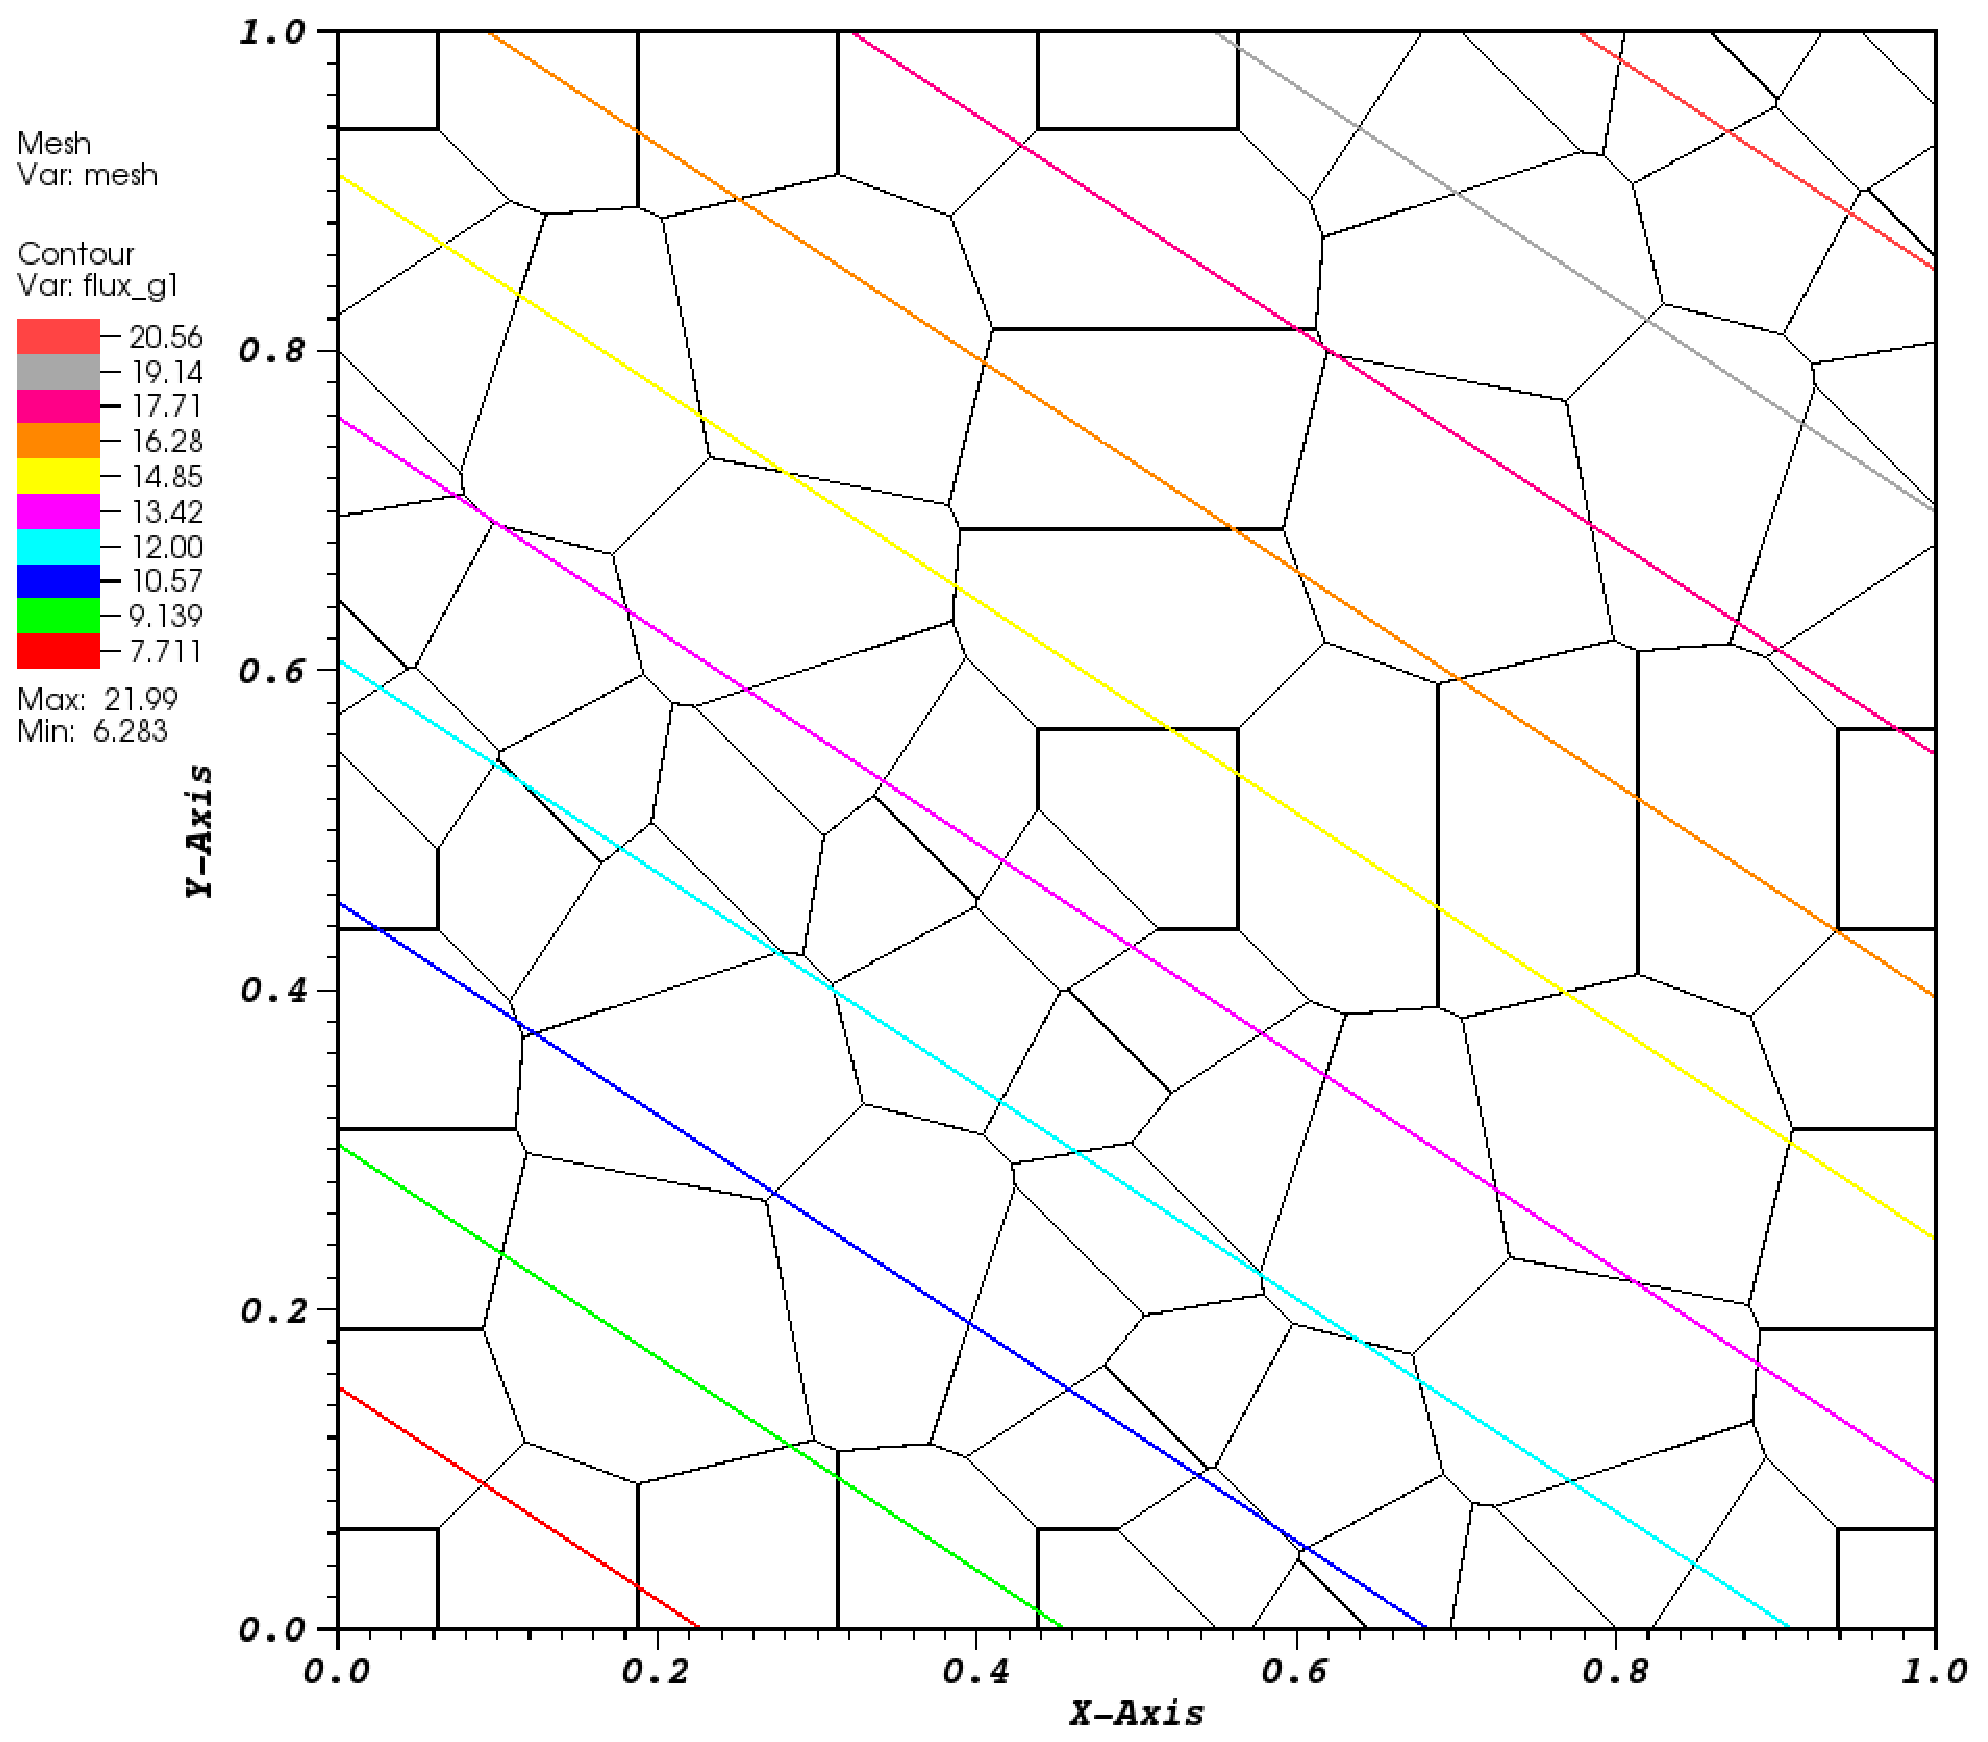
\includegraphics[width=\textwidth]{figures/sec_BF/smooth_poly_PWLD_k1.eps}
		\caption{}
	\end{subfigure}
	\vfill
	\begin{subfigure}[b]{0.45\textwidth}
		\centering
		\label{subfig::z_quad_pwld_lin_sol}
		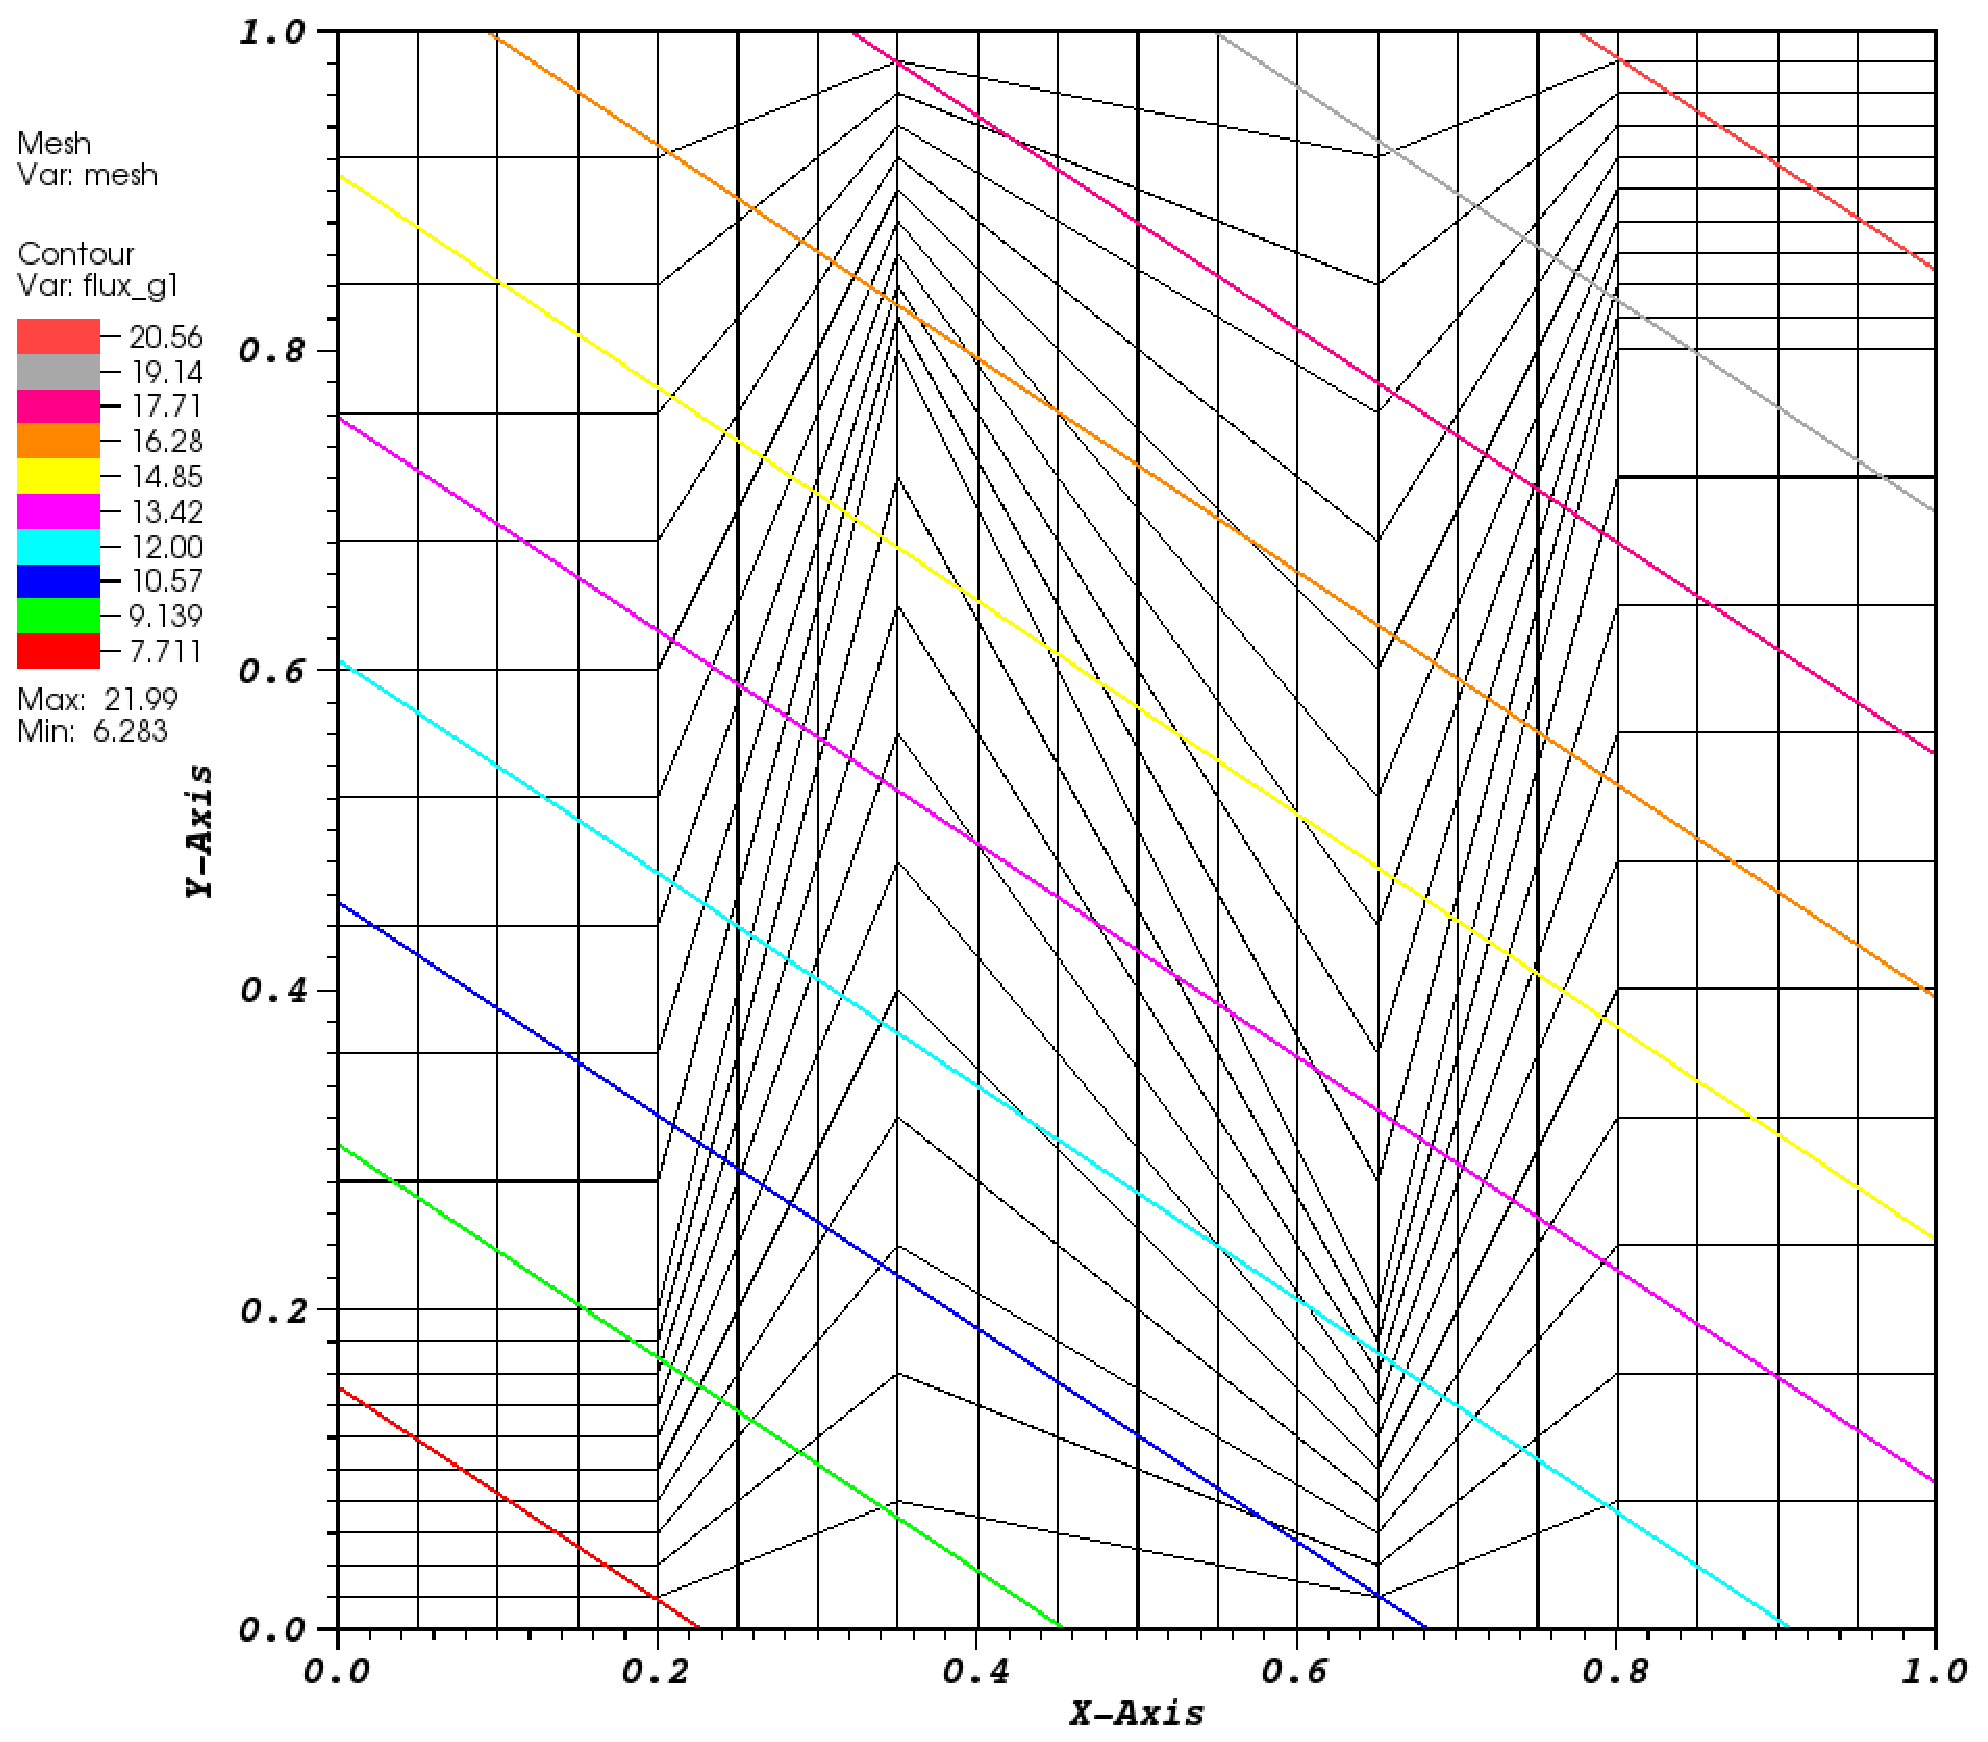
\includegraphics[width=\textwidth]{figures/sec_BF/z_quad_PWLD_k1.eps}
		\caption{}
	\end{subfigure}
	\hfill
	\begin{subfigure}[b]{0.45\textwidth}
		\centering
		\label{subfig::z_poly_pwld_lin_sol}
		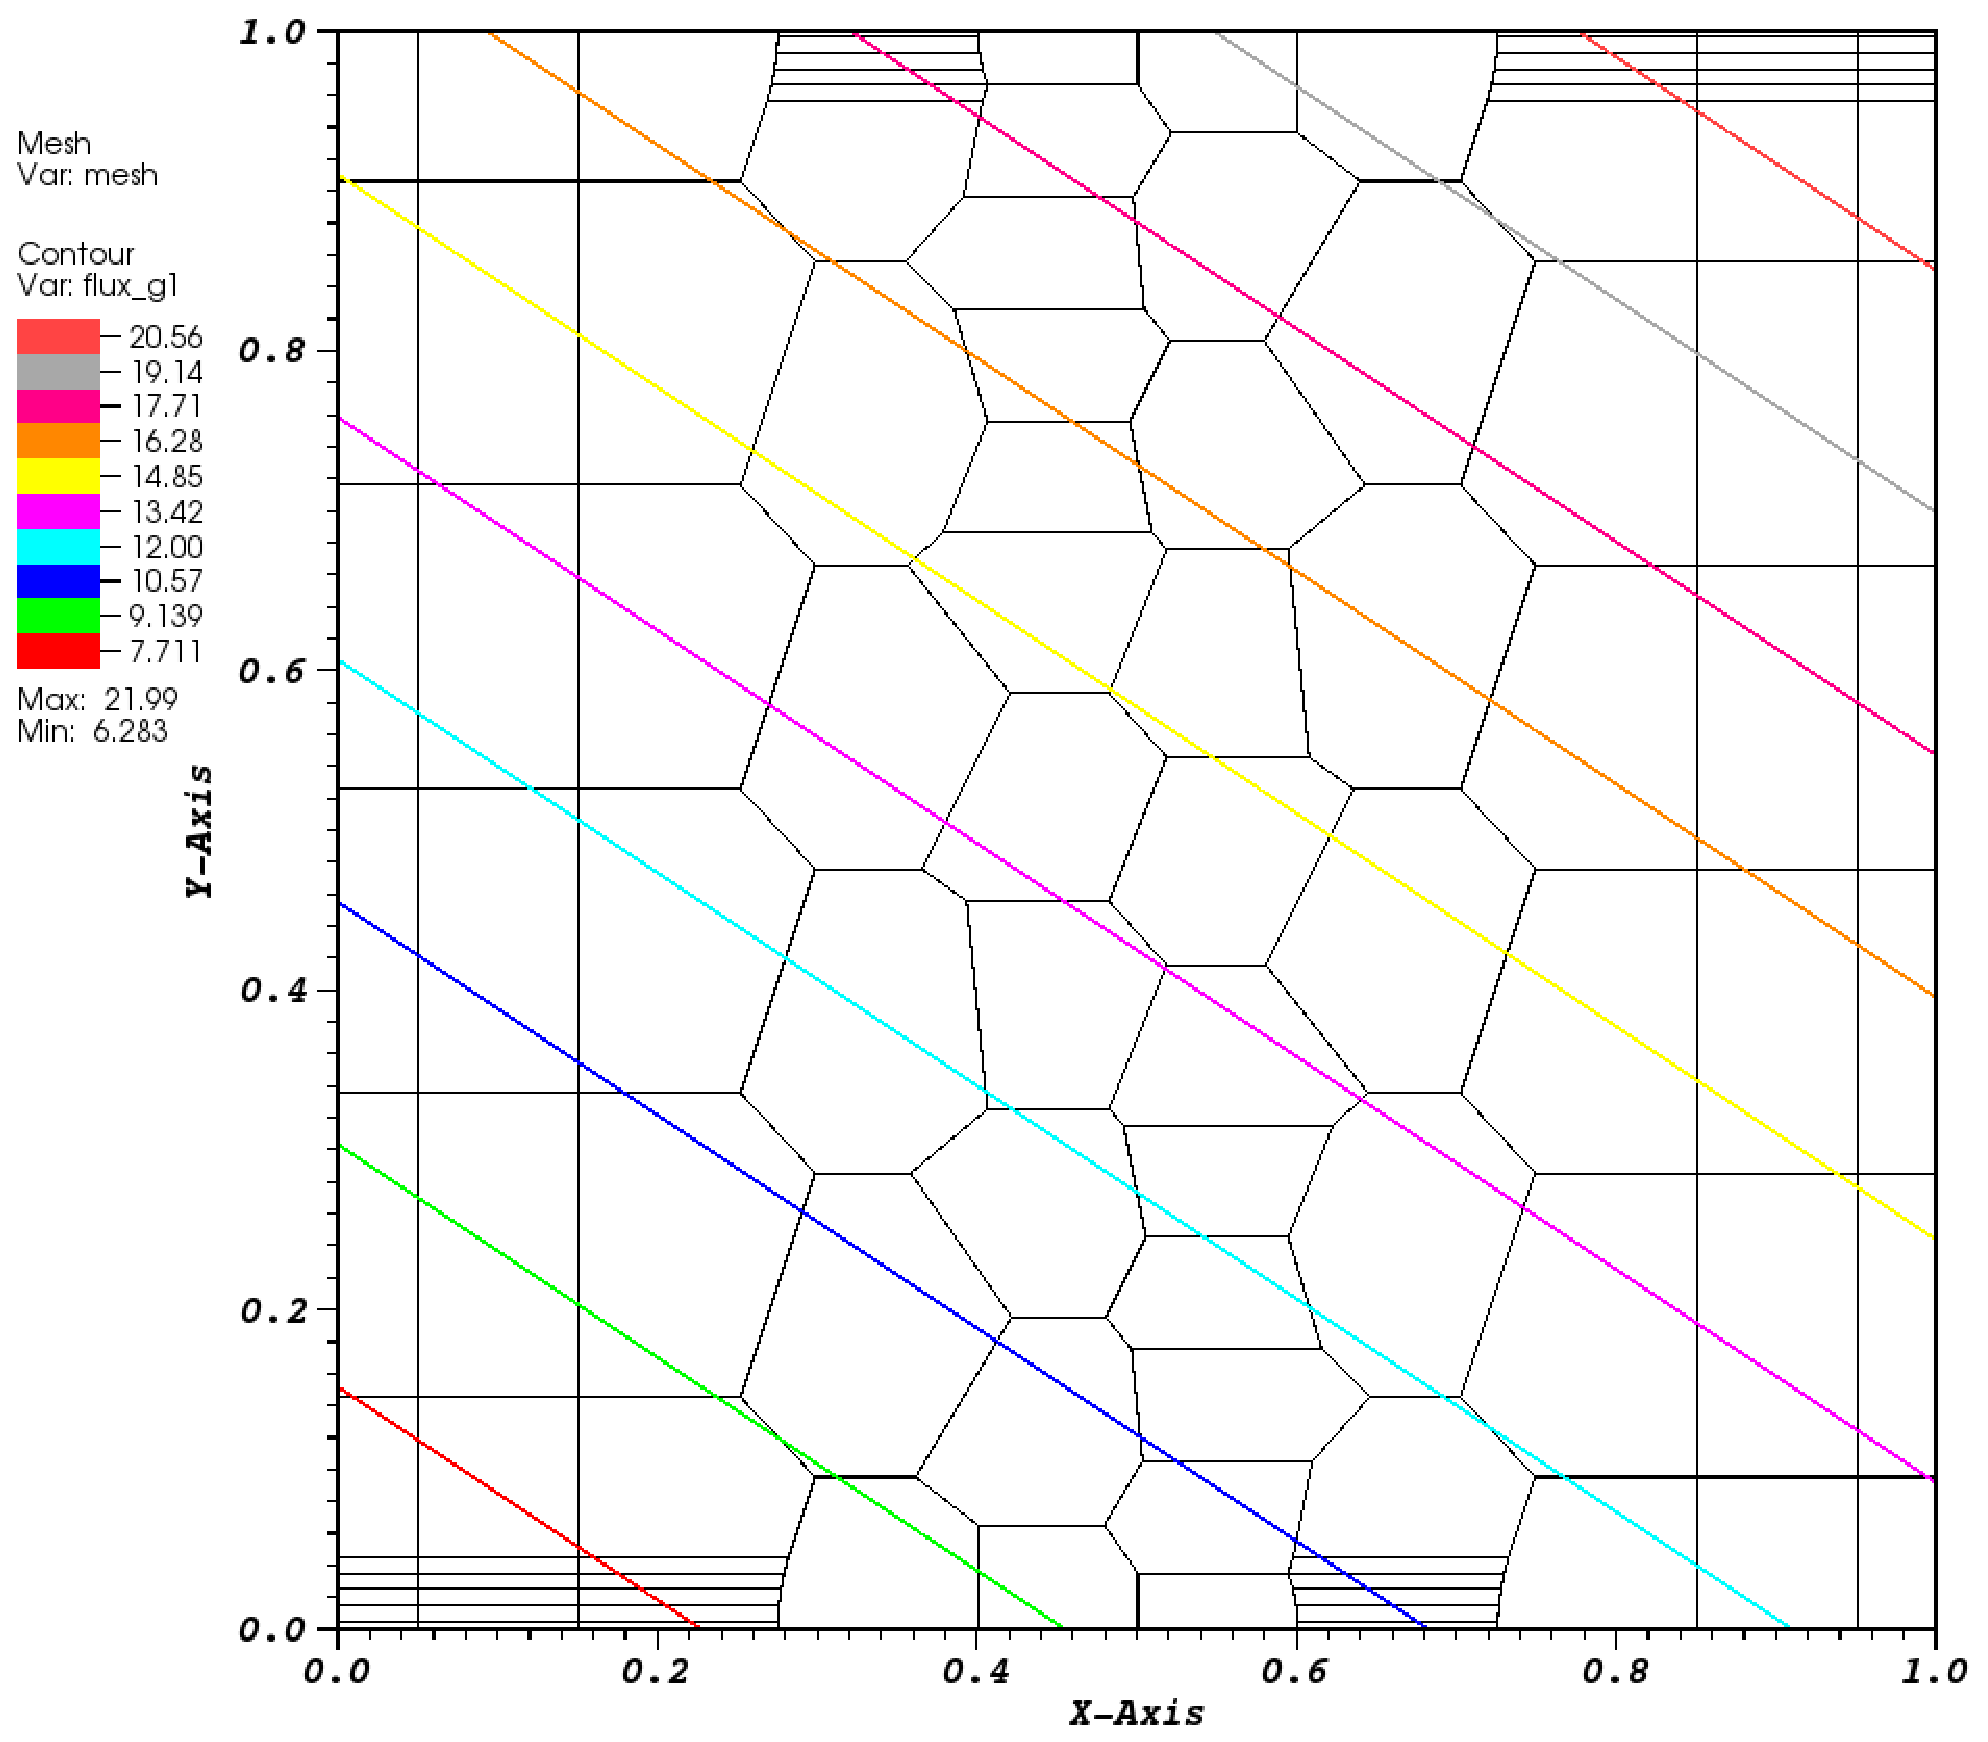
\includegraphics[width=\textwidth]{figures/sec_BF/z_poly_PWLD_k1.eps}
		\caption{}
	\end{subfigure}
\caption{Contour plots of the exactly-linear solution with the PWL basis functions on (a) cartesian mesh, (b) ordered-triangular mesh, (c) quadrilateral shestakov mesh, (d) sinusoidal polygonal mesh, (e) quadrilateral z-mesh, and (f) polygonal z-mesh.}
\label{fig::BF_Results_Linear_pwld_sol}
\end{figure}

\begin{figure}
\centering
	\begin{subfigure}[b]{0.45\textwidth}
		\centering
		\label{subfig::cart_mv_lin_sol}
		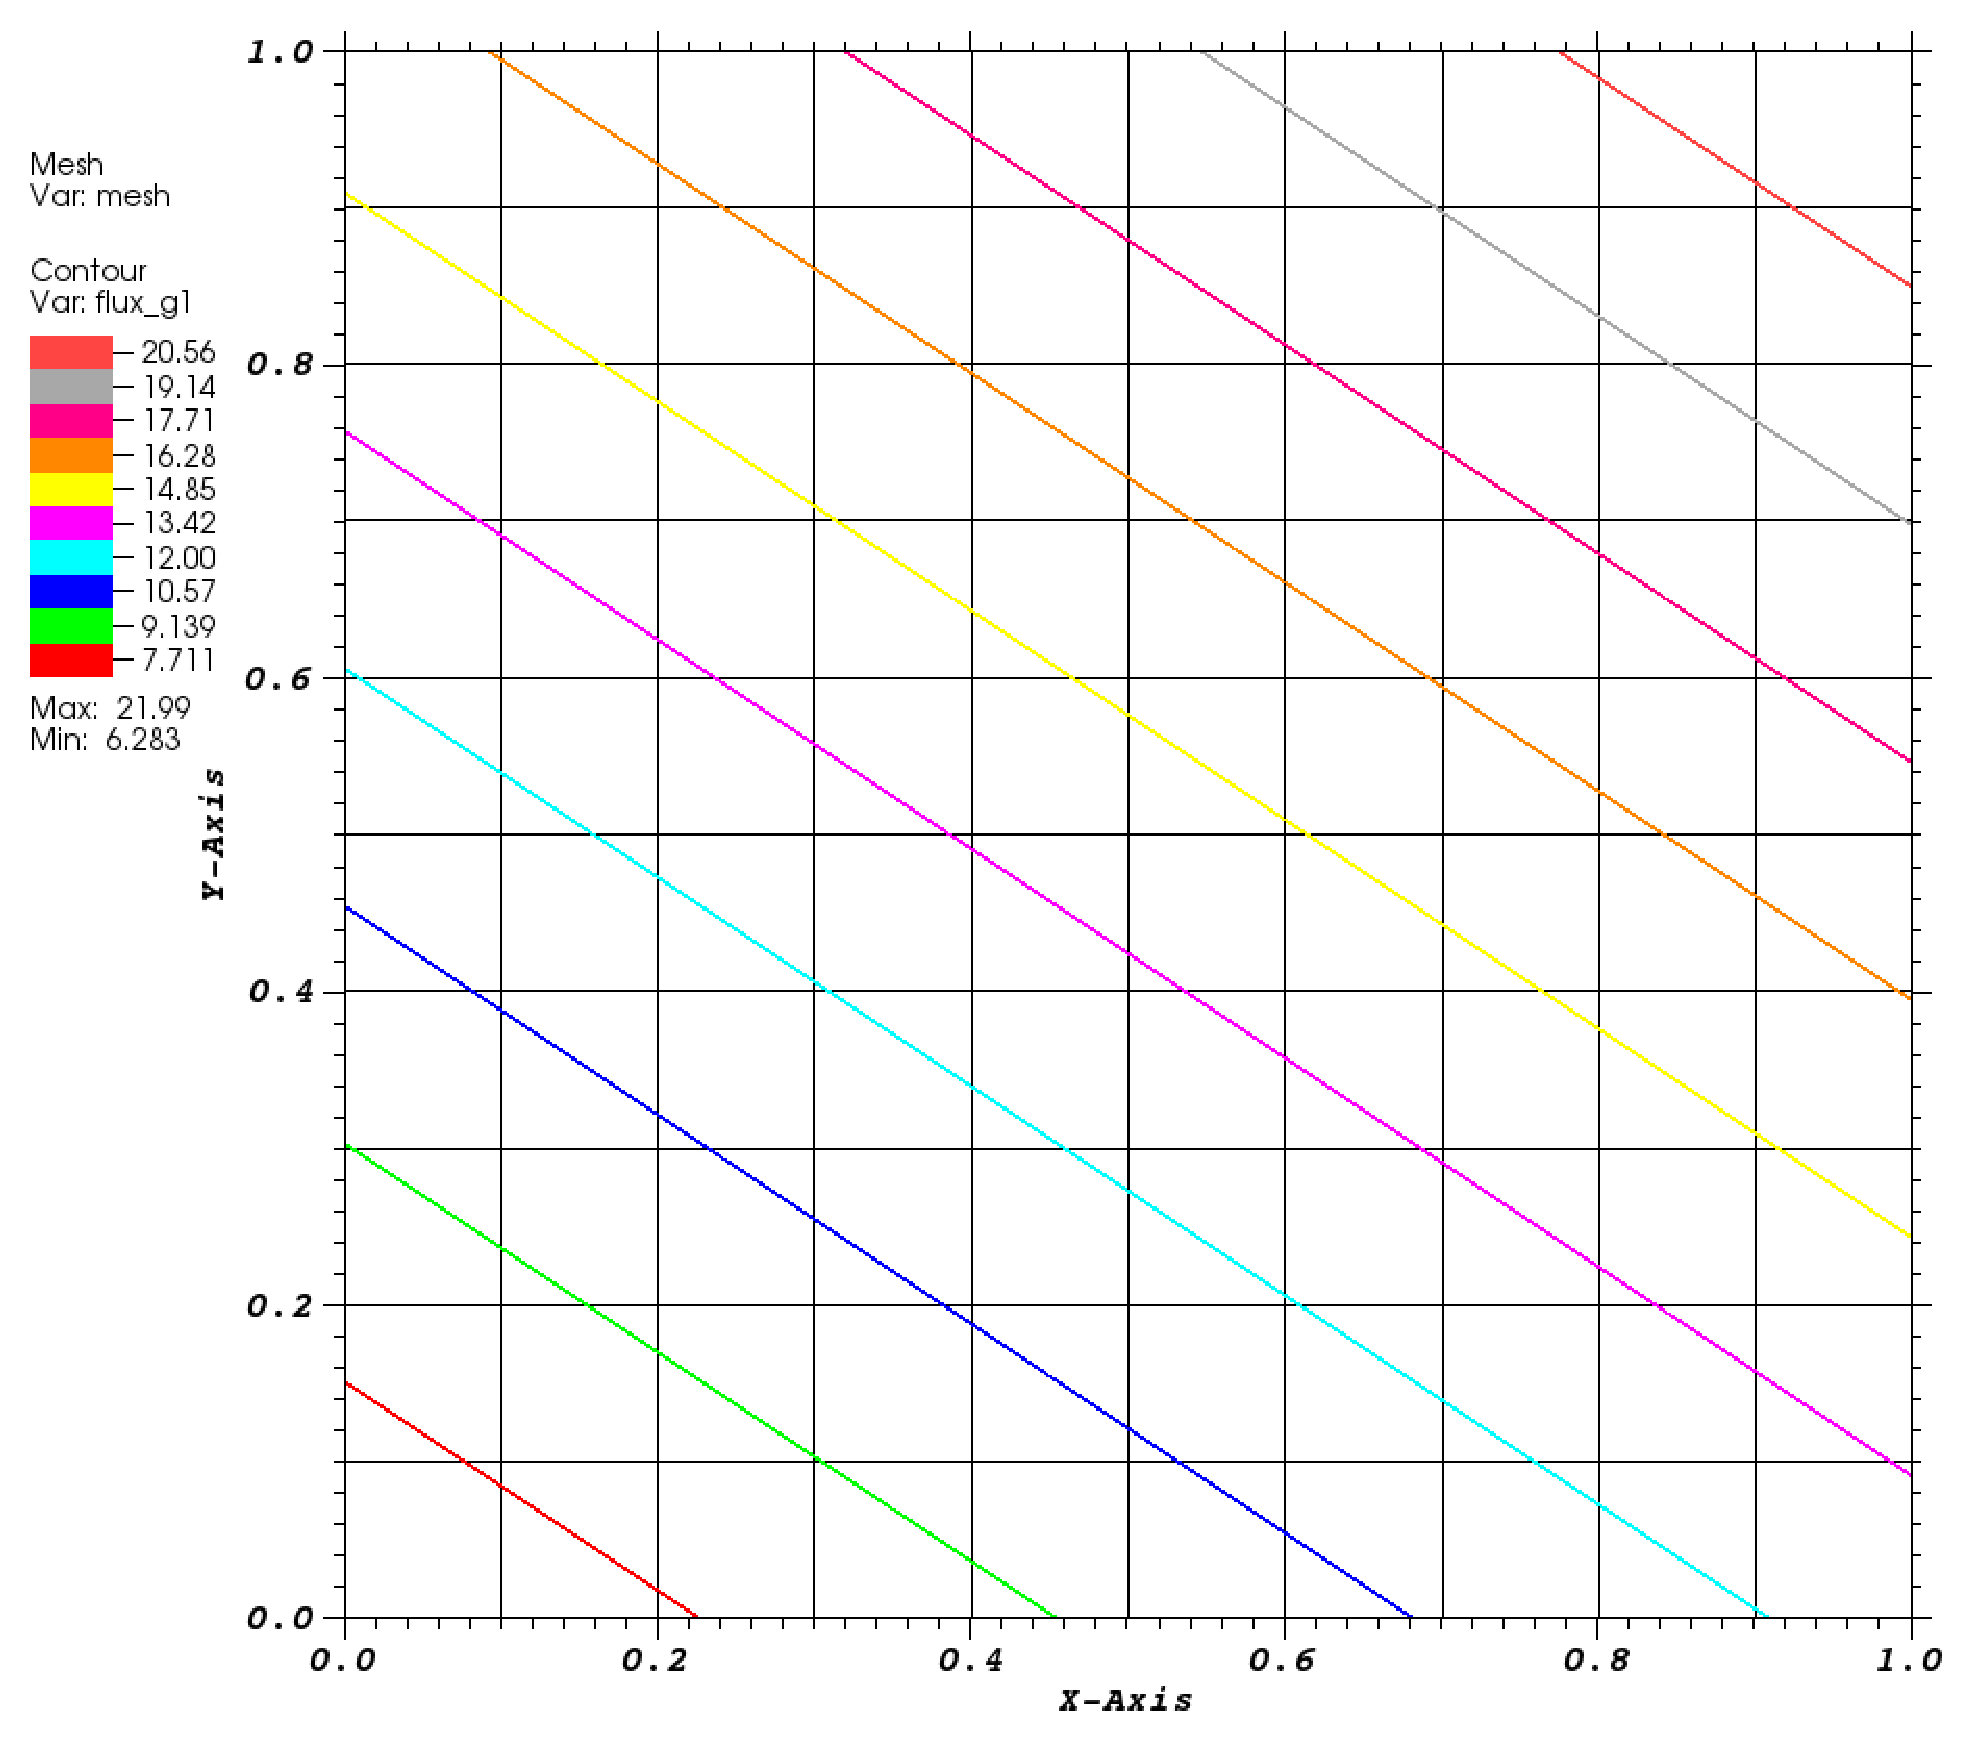
\includegraphics[width=\textwidth]{figures/sec_BF/cart_MV_k1.eps}
		\caption{}
	\end{subfigure}
	\hfill
	\begin{subfigure}[b]{0.45\textwidth}
		\centering
		\label{subfig::tri_mv_lin_sol}
		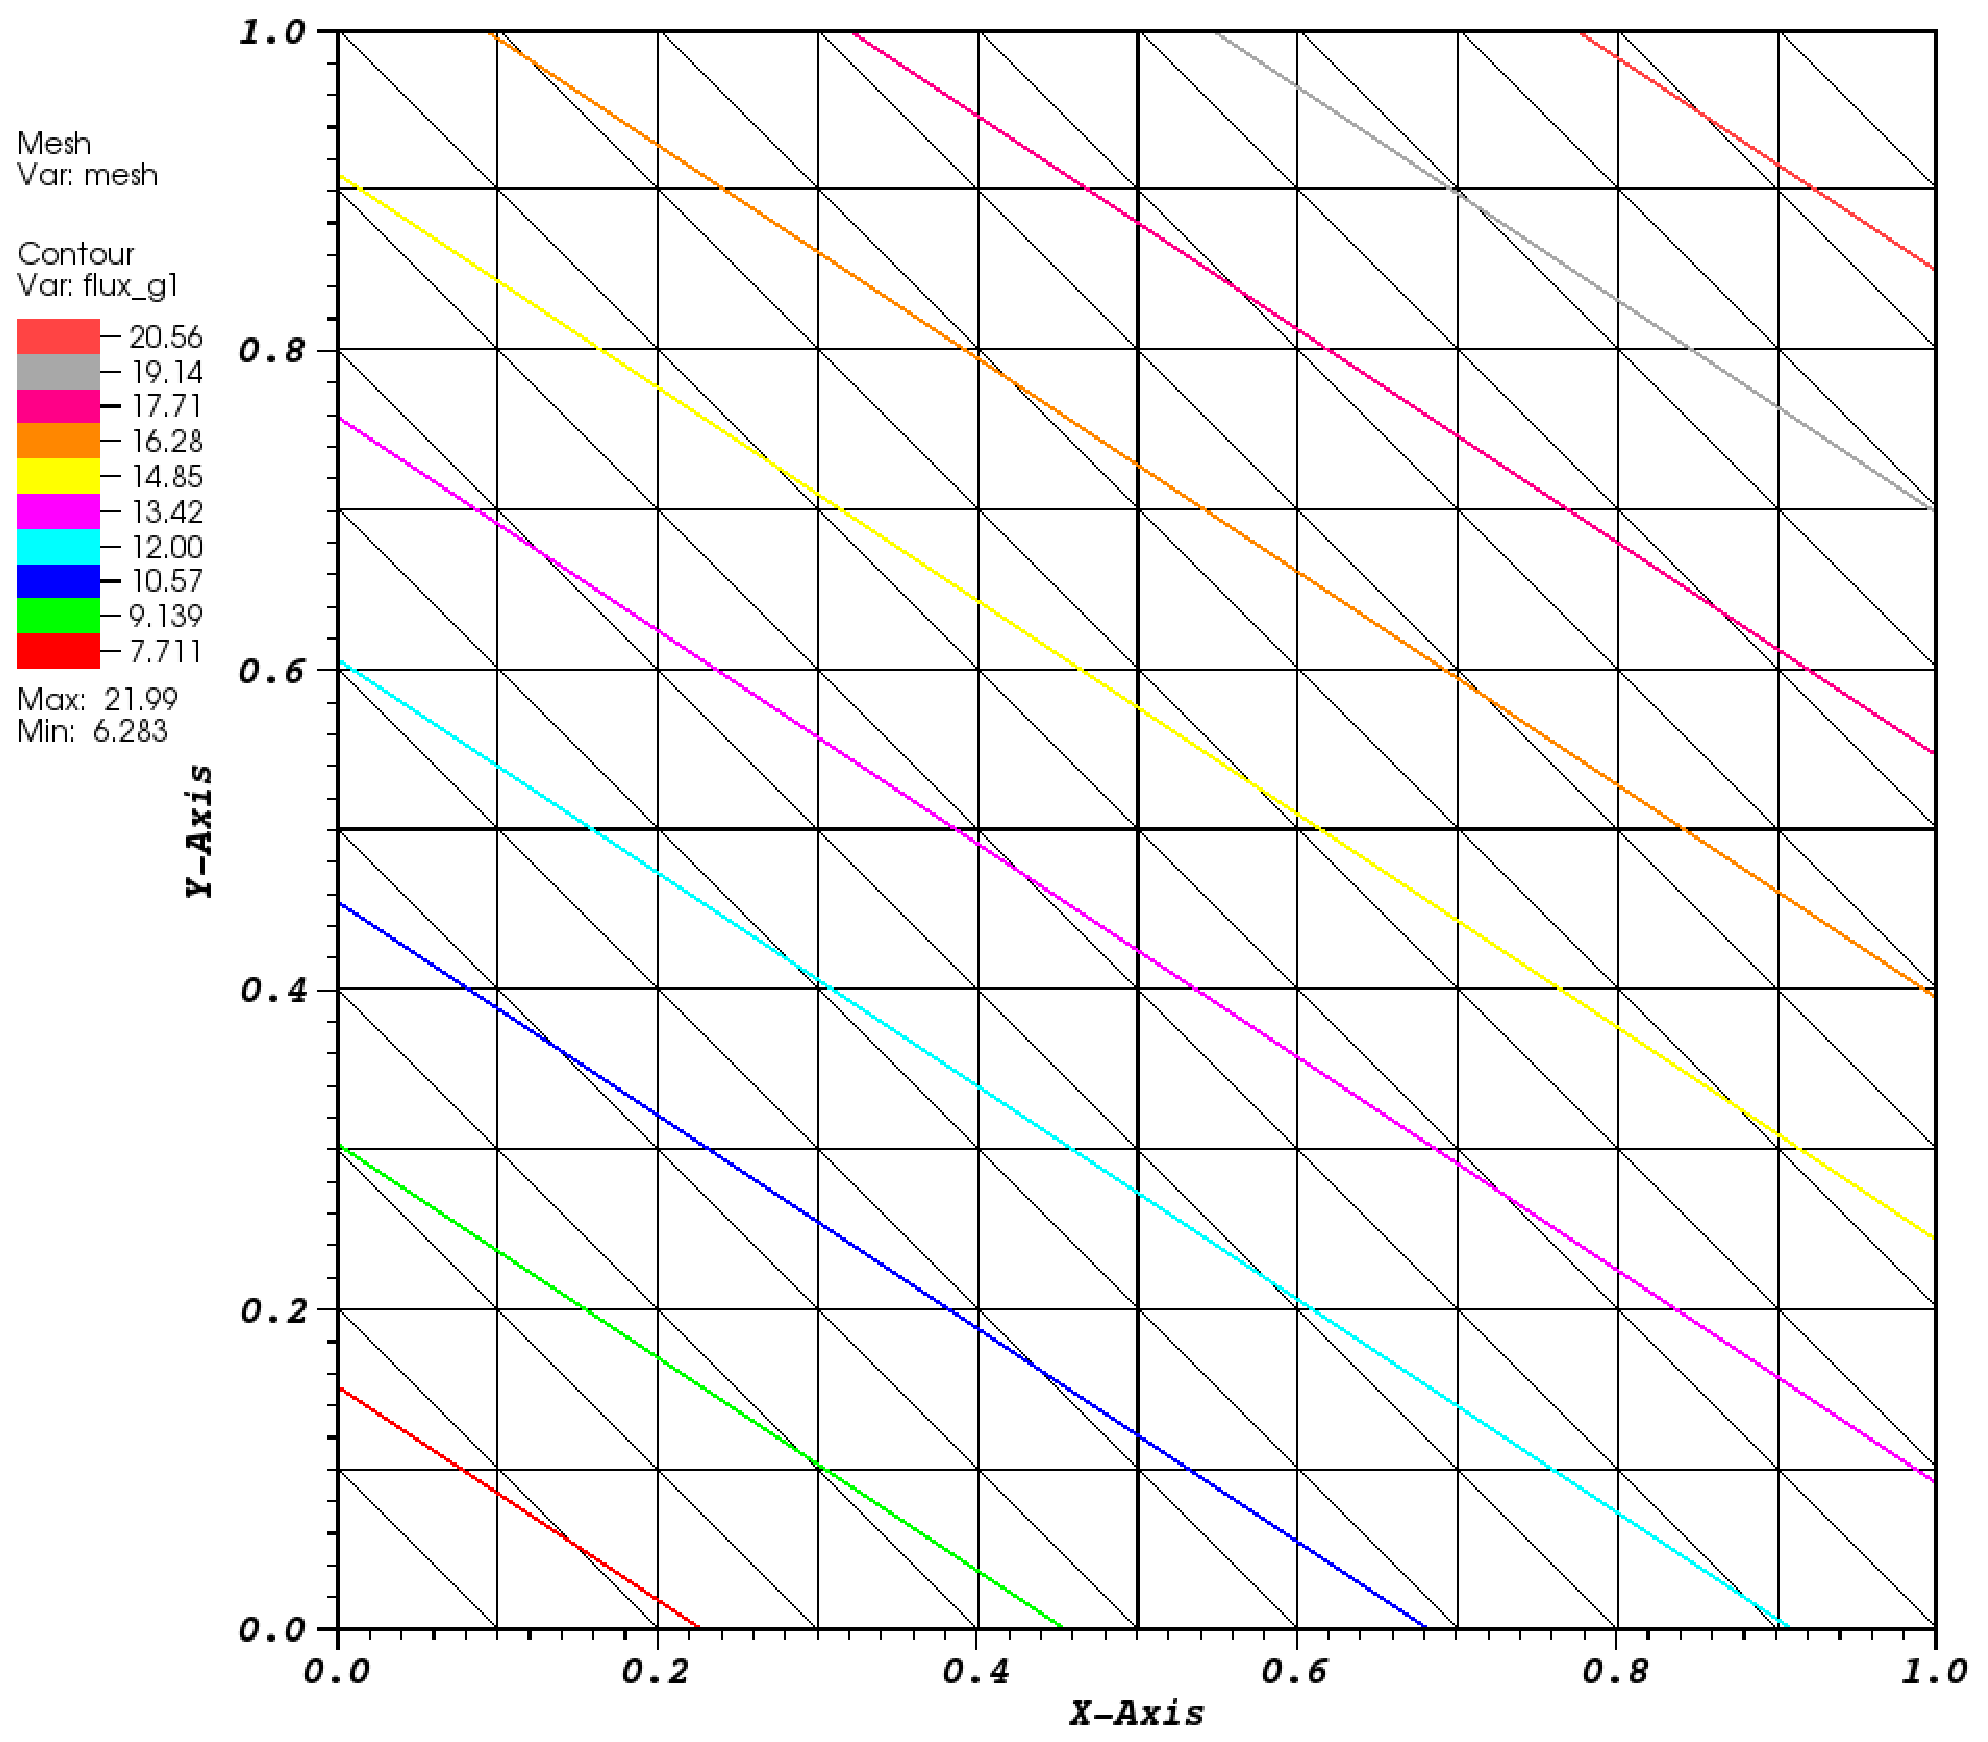
\includegraphics[width=\textwidth]{figures/sec_BF/tri_MV_k1.eps}
		\caption{}
	\end{subfigure}
	\vfill
	\begin{subfigure}[b]{0.45\textwidth}
		\centering
		\label{subfig::shes_quad_mv_lin_sol}
		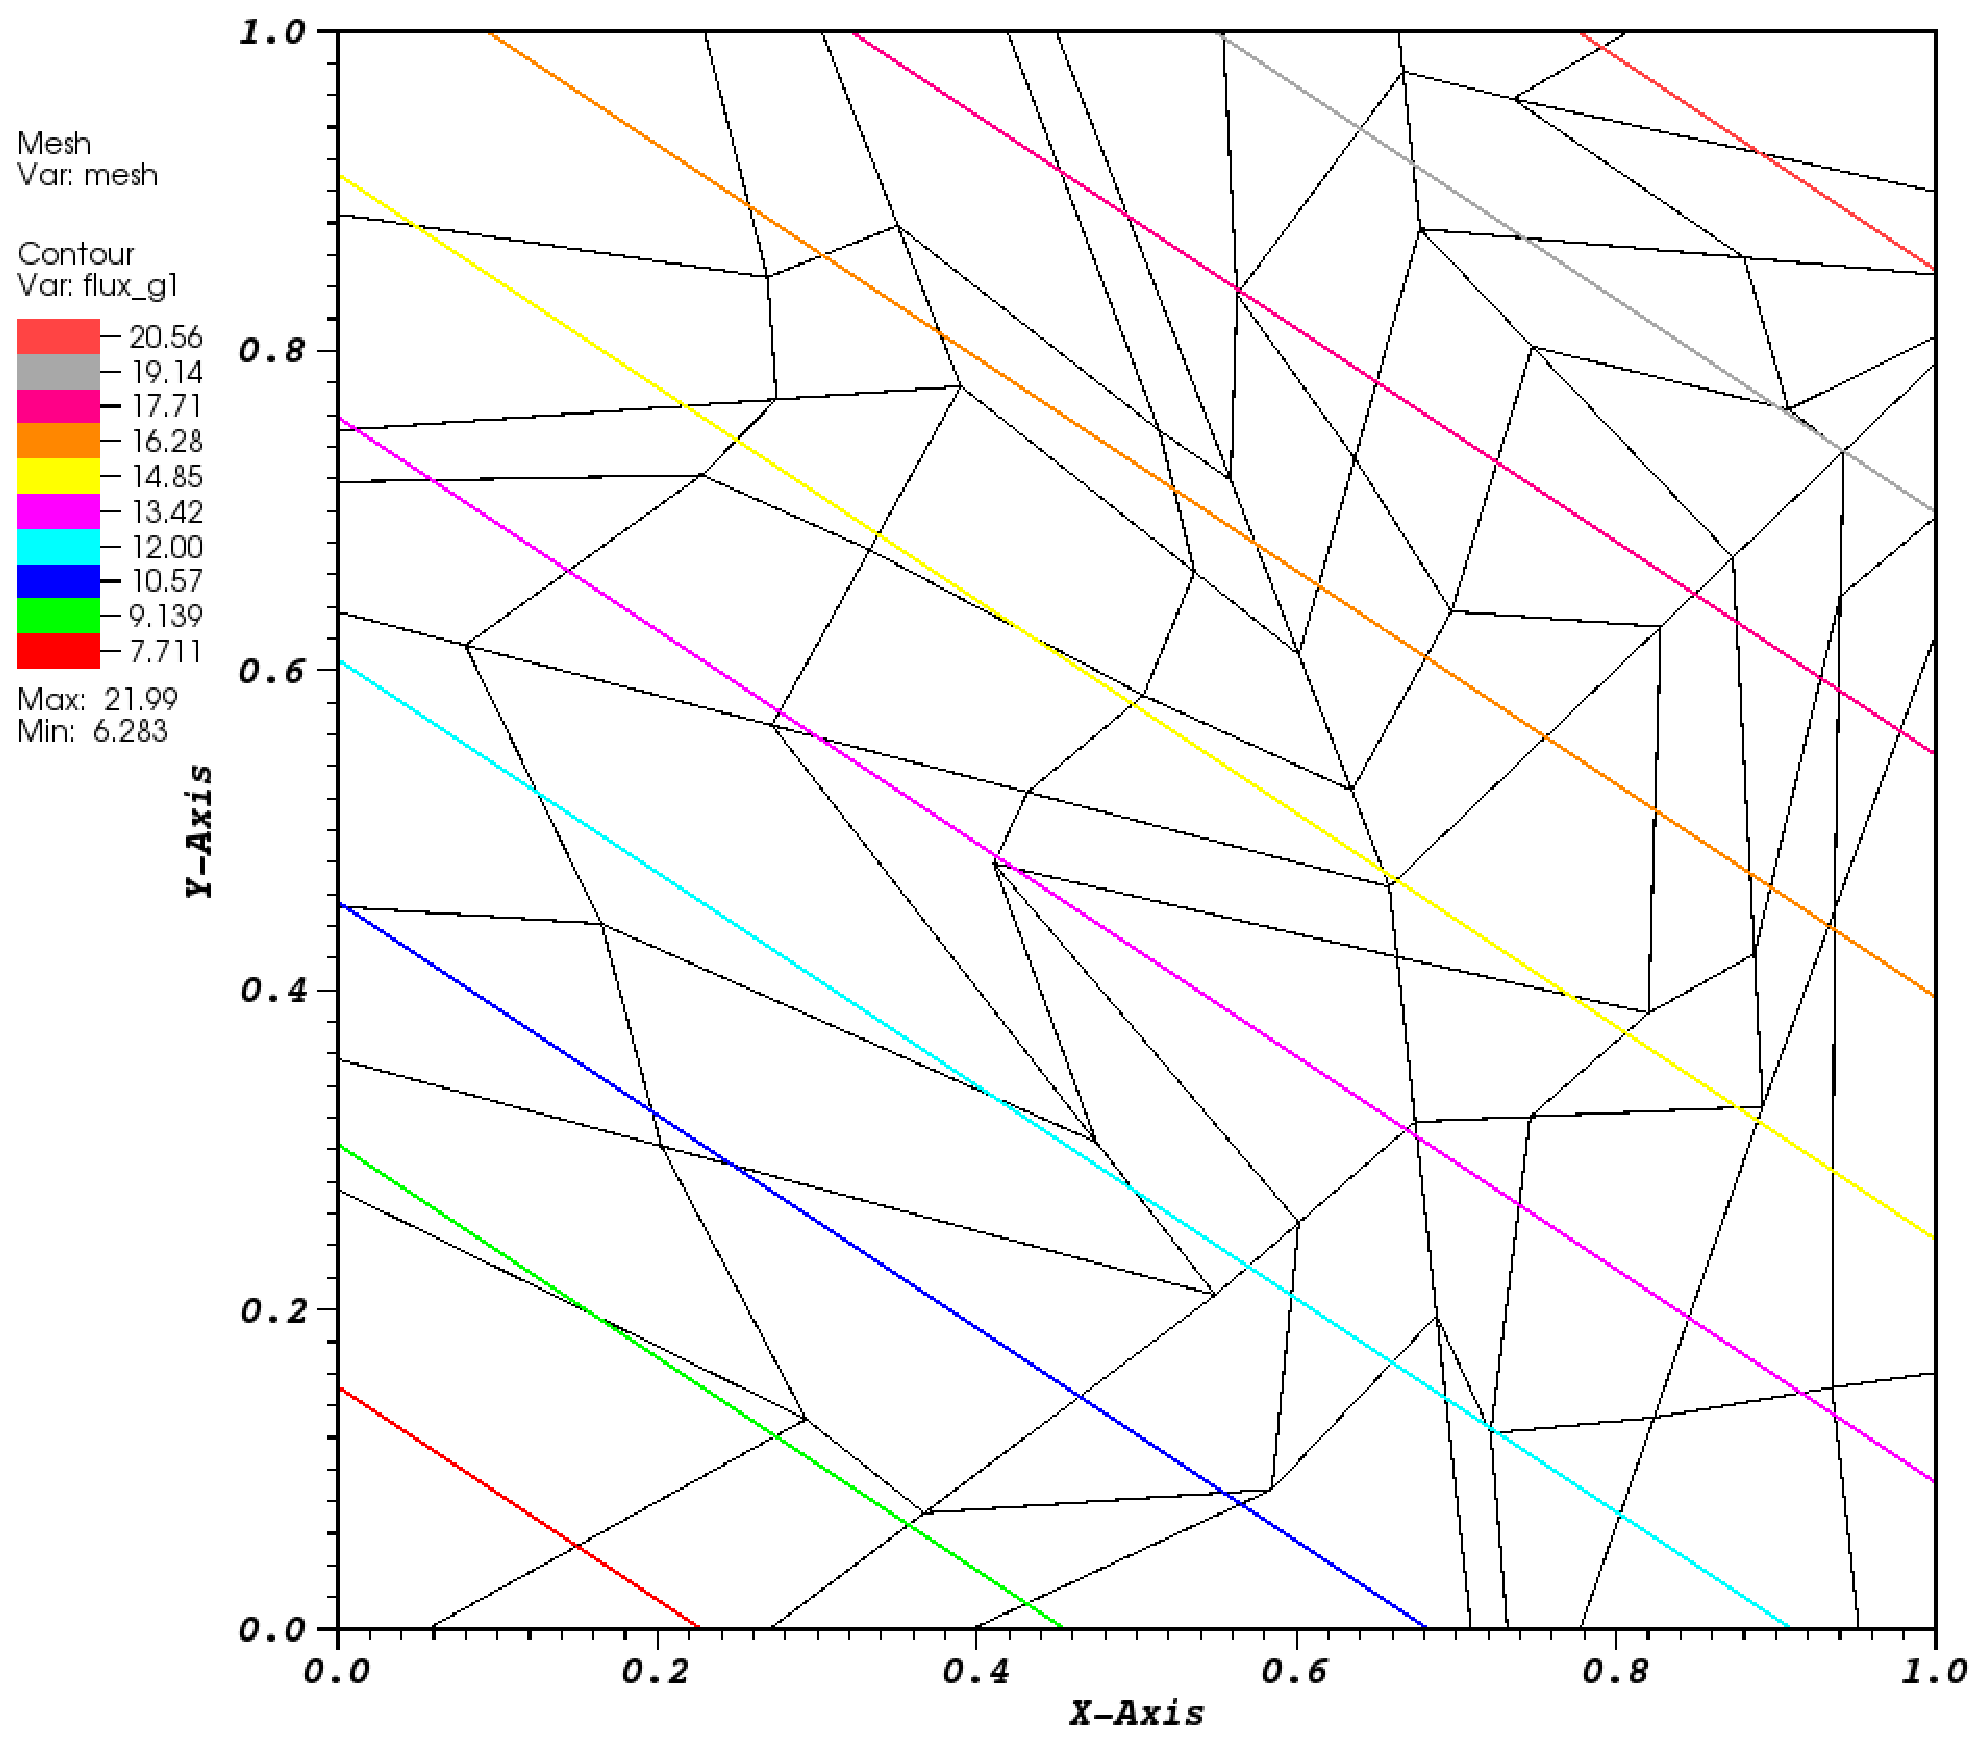
\includegraphics[width=\textwidth]{figures/sec_BF/shes_quad_MV_k1.eps}
		\caption{}
	\end{subfigure}
	\hfill
	\begin{subfigure}[b]{0.45\textwidth}
		\centering
		\label{subfig::smooth_poly_mv_lin_sol}
		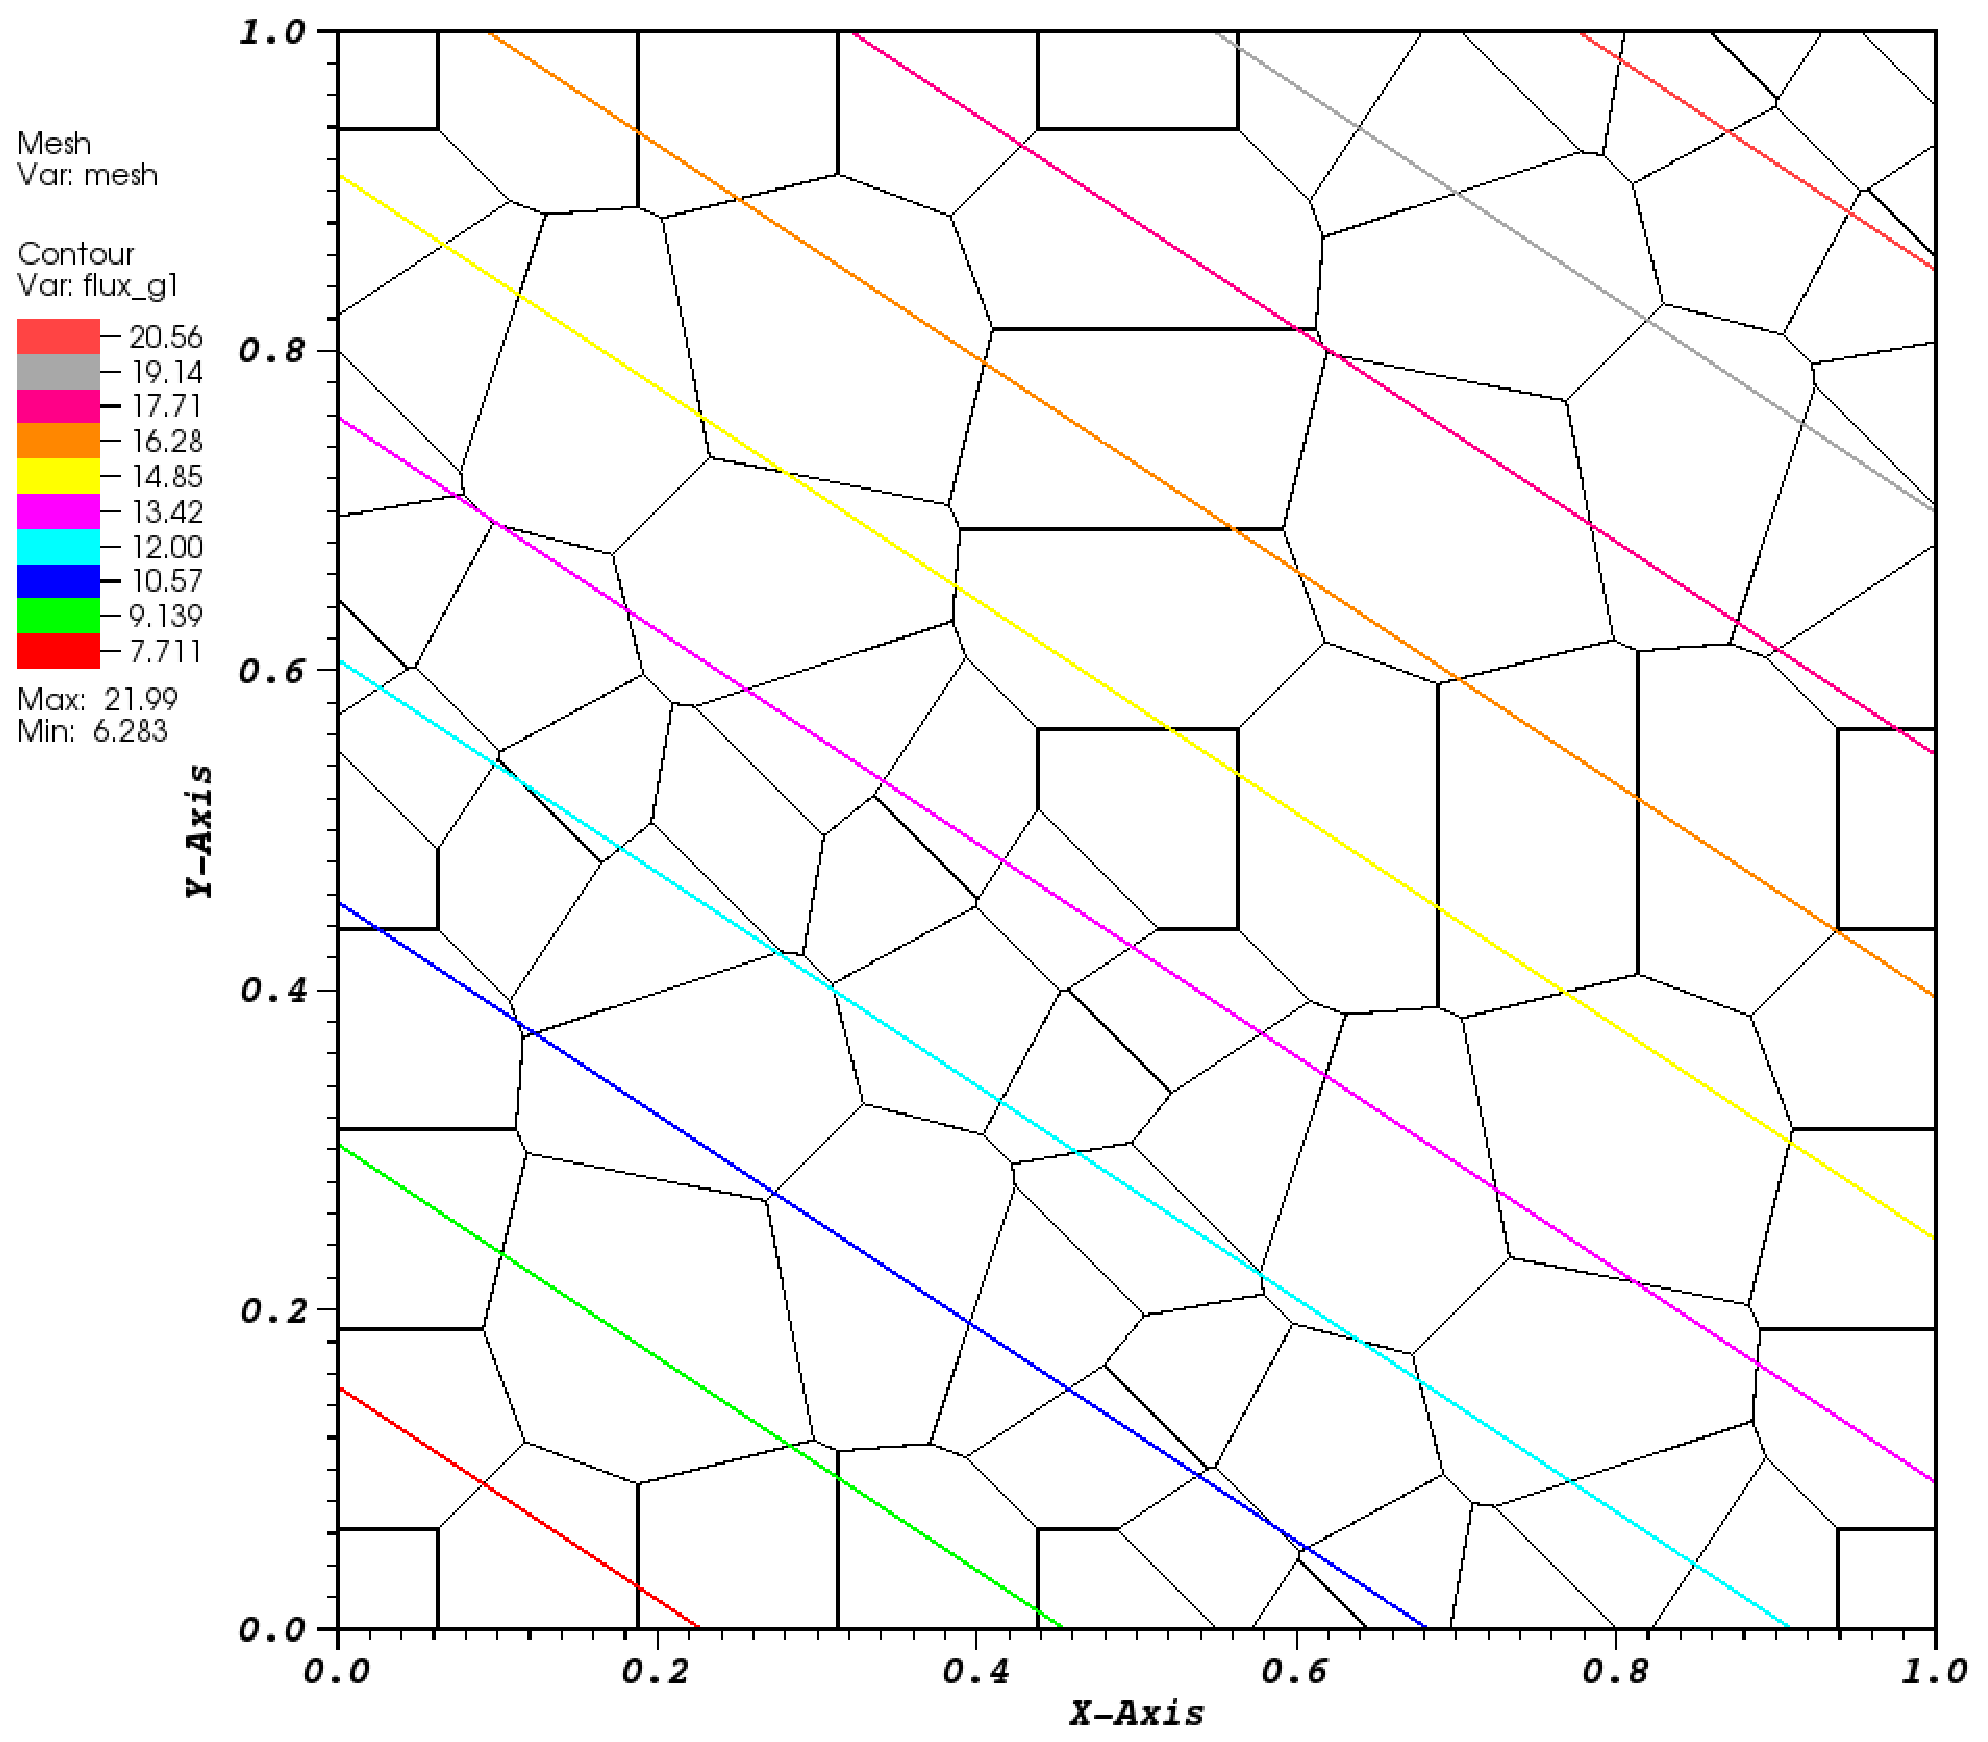
\includegraphics[width=\textwidth]{figures/sec_BF/smooth_poly_MV_k1.eps}
		\caption{}
	\end{subfigure}
	\vfill
	\begin{subfigure}[b]{0.45\textwidth}
		\centering
		\label{subfig::z_quad_mv_lin_sol}
		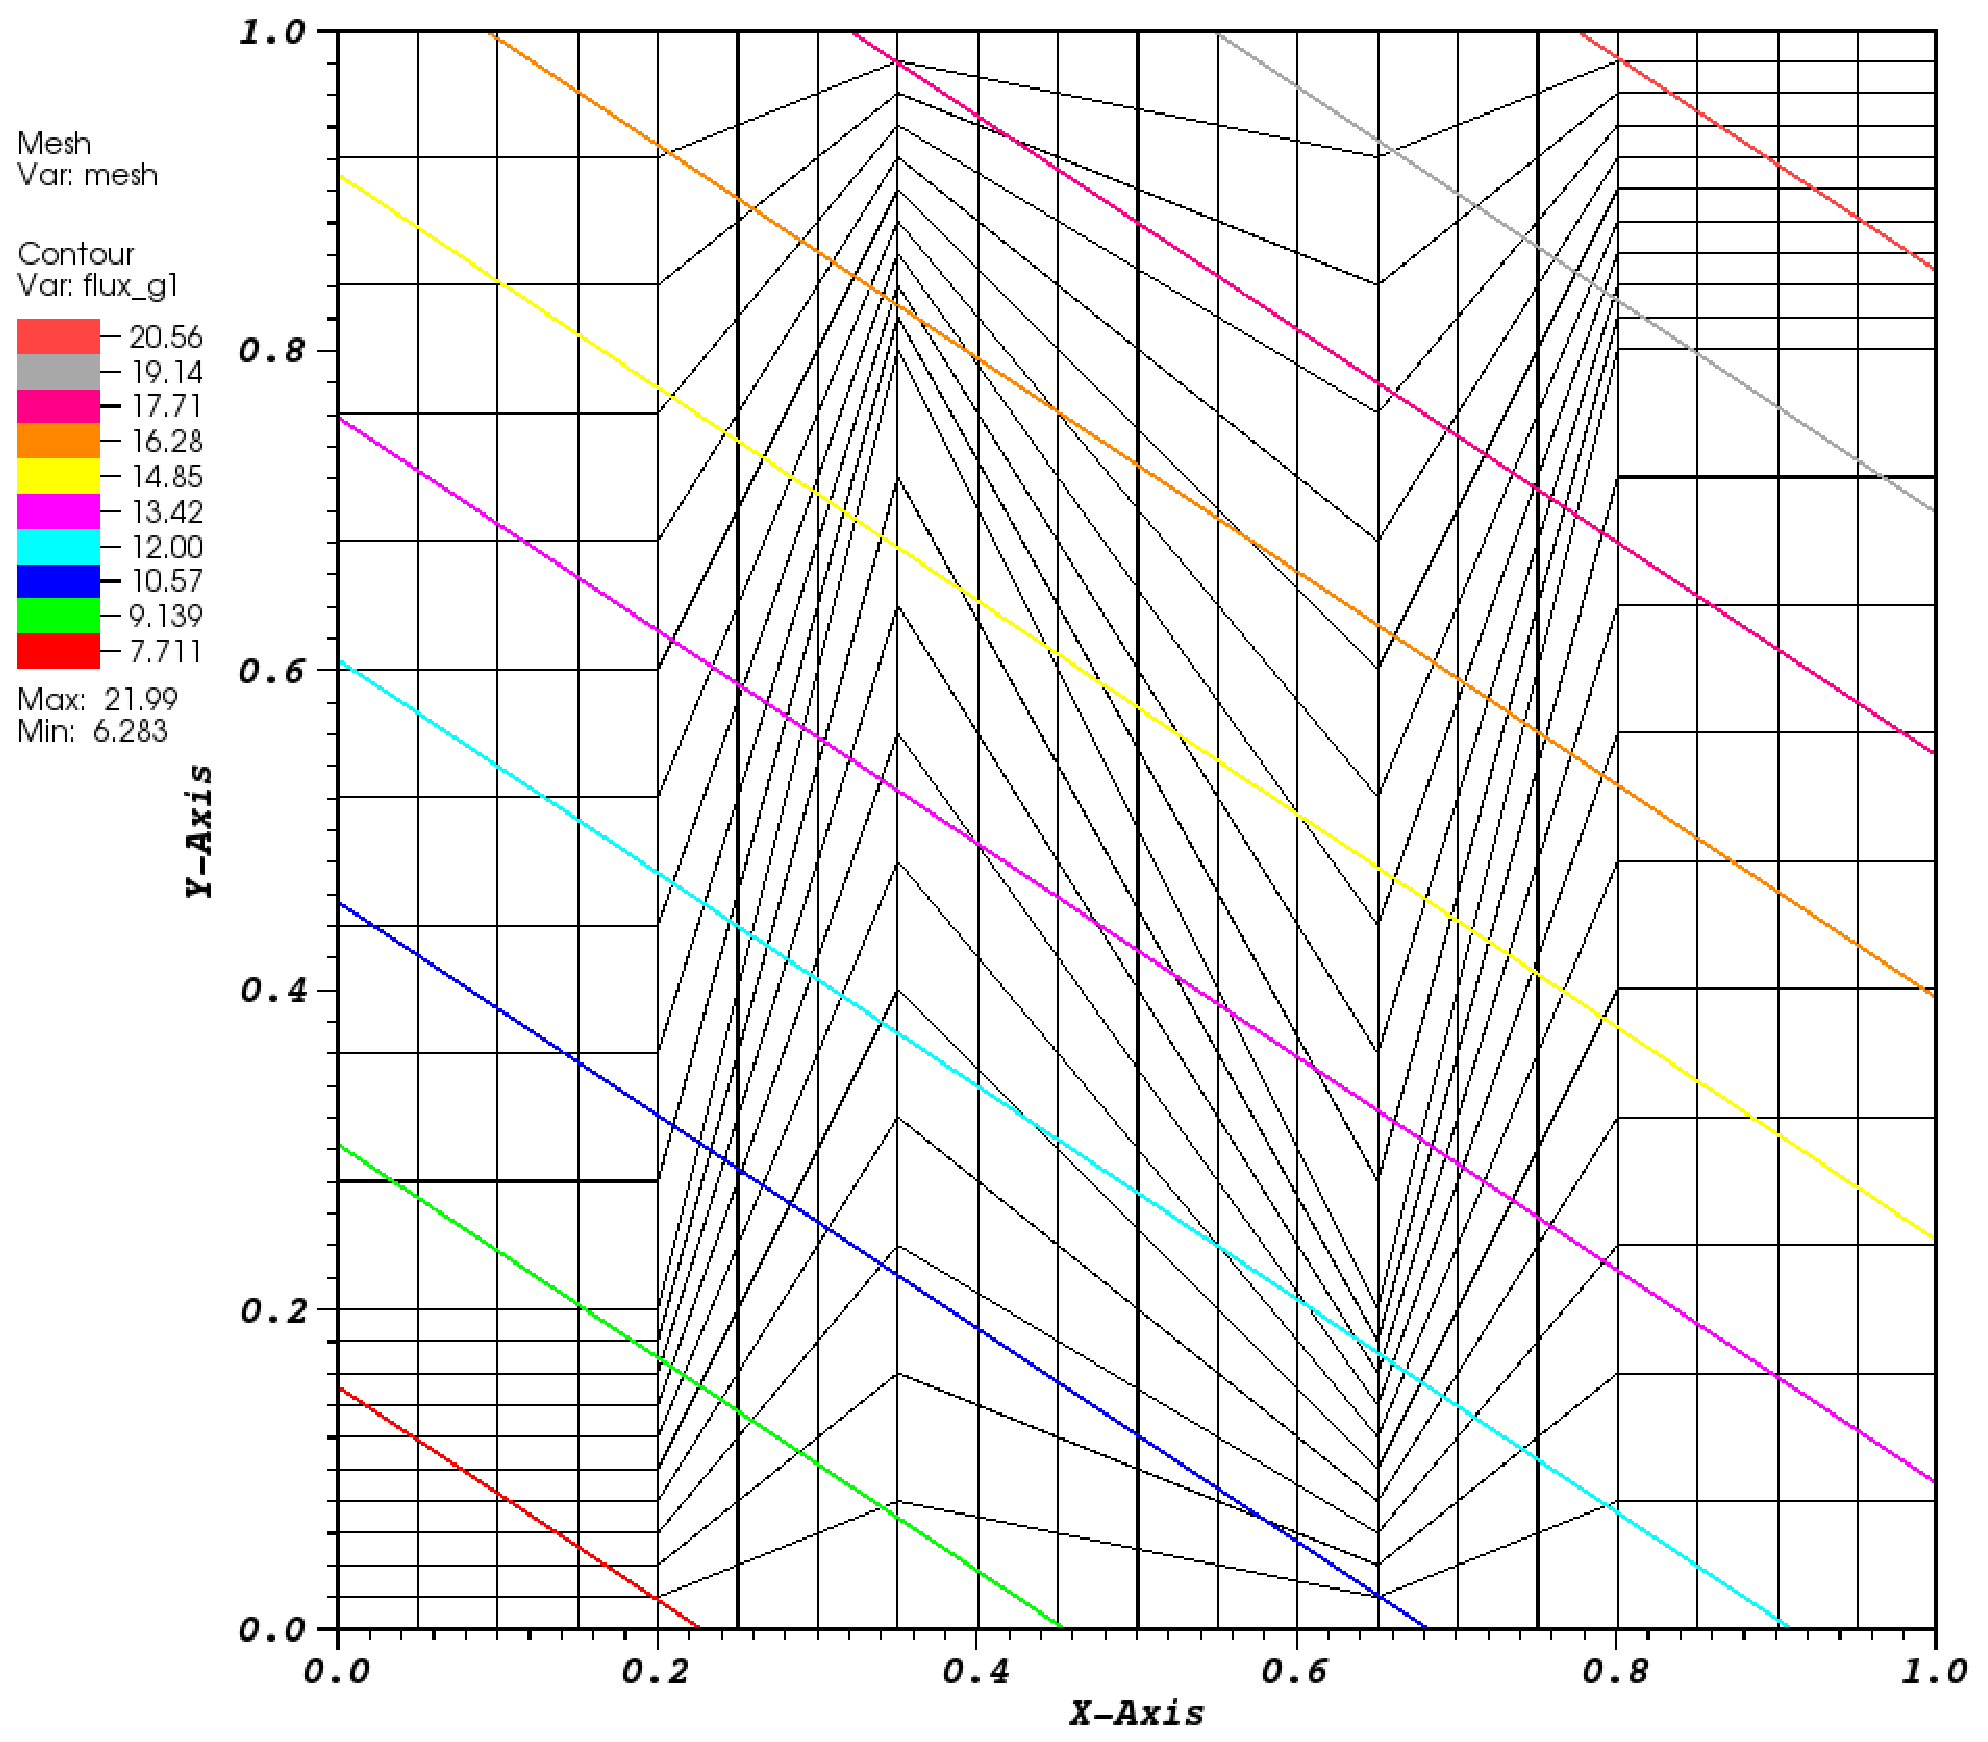
\includegraphics[width=\textwidth]{figures/sec_BF/z_quad_MV_k1.eps}
		\caption{}
	\end{subfigure}
	\hfill
	\begin{subfigure}[b]{0.45\textwidth}
		\centering
		\label{subfig::z_poly_mv_lin_sol}
		\includegraphics[width=\textwidth]{figures/sec_BF/z_poly_MV_k1.eps}
		\caption{}
	\end{subfigure}
\caption{Contour plots of the exactly-linear solution with the mean value basis functions on (a) cartesian mesh, (b) ordered-triangular mesh, (c) quadrilateral shestakov mesh, (d) sinusoidal polygonal mesh, (e) quadrilateral z-mesh, and (f) polygonal z-mesh.}
\label{fig::BF_Results_Linear_mv_sol}
\end{figure}

\begin{figure}
\centering
	\begin{subfigure}[b]{0.45\textwidth}
		\centering
		\label{subfig::cart_me_k1_lin_sol}
		\includegraphics[width=\textwidth]{figures/sec_BF/cart_MAXENT_k1.eps}
		\caption{}
	\end{subfigure}
	\hfill
	\begin{subfigure}[b]{0.45\textwidth}
		\centering
		\label{subfig::tri_me_k1_lin_sol}
		\includegraphics[width=\textwidth]{figures/sec_BF/tri_MAXENT_k1.eps}
		\caption{}
	\end{subfigure}
	\vfill
	\begin{subfigure}[b]{0.45\textwidth}
		\centering
		\label{subfig::shes_quad_me_k1_lin_sol}
		\includegraphics[width=\textwidth]{figures/sec_BF/shes_quad_MAXENT_k1.eps}
		\caption{}
	\end{subfigure}
	\hfill
	\begin{subfigure}[b]{0.45\textwidth}
		\centering
		\label{subfig::smooth_poly_me_k1_lin_sol}
		\includegraphics[width=\textwidth]{figures/sec_BF/smooth_poly_MAXENT_k1.eps}
		\caption{}
	\end{subfigure}
	\vfill
	\begin{subfigure}[b]{0.45\textwidth}
		\centering
		\label{subfig::z_quad_me_k1_lin_sol}
		\includegraphics[width=\textwidth]{figures/sec_BF/z_quad_MAXENT_k1.eps}
		\caption{}
	\end{subfigure}
	\hfill
	\begin{subfigure}[b]{0.45\textwidth}
		\centering
		\label{subfig::z_poly_me_k1_lin_sol}
		\includegraphics[width=\textwidth]{figures/sec_BF/z_poly_MAXENT_k1.eps}
		\caption{}
	\end{subfigure}
\caption{Contour plots of the exactly-linear solution with the linear maximum entropy basis functions on (a) cartesian mesh, (b) ordered-triangular mesh, (c) quadrilateral shestakov mesh, (d) sinusoidal polygonal mesh, (e) quadrilateral z-mesh, and (f) polygonal z-mesh.}
\label{fig::BF_Results_Linear_me1_sol}
\end{figure}

\begin{figure}
\centering
	\begin{subfigure}[b]{0.45\textwidth}
		\centering
		\label{subfig::cart_me_k2_lin_sol}
		\includegraphics[width=\textwidth]{figures/sec_BF/cart_MAXENT_k2.eps}
		\caption{}
	\end{subfigure}
	\hfill
	\begin{subfigure}[b]{0.45\textwidth}
		\centering
		\label{subfig::tri_me_k2_lin_sol}
		\includegraphics[width=\textwidth]{figures/sec_BF/tri_MAXENT_k2.eps}
		\caption{}
	\end{subfigure}
	\vfill
	\begin{subfigure}[b]{0.45\textwidth}
		\centering
		\label{subfig::shes_quad_me_k2_lin_sol}
		\includegraphics[width=\textwidth]{figures/sec_BF/shes_quad_MAXENT_k2.eps}
		\caption{}
	\end{subfigure}
	\hfill
	\begin{subfigure}[b]{0.45\textwidth}
		\centering
		\label{subfig::smooth_poly_me_k2_lin_sol}
		\includegraphics[width=\textwidth]{figures/sec_BF/smooth_poly_MAXENT_k2.eps}
		\caption{}
	\end{subfigure}
	\vfill
	\begin{subfigure}[b]{0.45\textwidth}
		\centering
		\label{subfig::z_quad_me_k2_lin_sol}
		\includegraphics[width=\textwidth]{figures/sec_BF/z_quad_MAXENT_k2.eps}
		\caption{}
	\end{subfigure}
	\hfill
	\begin{subfigure}[b]{0.45\textwidth}
		\centering
		\label{subfig::z_poly_me_k2_lin_sol}
		\includegraphics[width=\textwidth]{figures/sec_BF/z_poly_MAXENT_k2.eps}
		\caption{}
	\end{subfigure}
\caption{Contour plots of the exactly-linear solution with the quadratic serendipity maximum entropy basis functions on (a) cartesian mesh, (b) ordered-triangular mesh, (c) quadrilateral shestakov mesh, (d) sinusoidal polygonal mesh, (e) quadrilateral z-mesh, and (f) polygonal z-mesh.}
\label{fig::BF_Results_Linear_me2_sol}
\end{figure}

%%%%%%%%%%%%%%%%%%%%%%%%%%%%%%%%%%%%%%%%%%%%%%%%%%%
%%%   SubSection - MMS
\subsection{Convergence Rate Analysis by the Method of Manufactured Solutions}
\label{sec::BF_Results_MMS}

The next numerical example we investigate involves calculating the convergence rate of the solution error via the method of manufactured solutions (MMS). Like MES, MMS enforces a given solution by use of a derived functional form for the driving source of the problem ($Q_{ext}$). However, unlike MES, we enforce a spatial solution that cannot be captured by the interpolation of the finite element space. Using a specification of the Bramble-Hilbert \cite{bramble1970estimation} lemma, the difference between the exact solution, $\Phi_e$, and the discretized solution, $\Phi_h$, residing in the Sobolev space, $W_{\mathcal{D}}^h \in \mathcal{T}_h$, for a given polynomial interpolation order, $k$, is

\begin{equation}
\label{eq::BF_Results_MMS_errnorm}
|| \Phi_{e} - \Phi_h || _{2}  \leq C \frac{h^{q+1/2}}{(k+1)^q} ,
\end{equation}

\noindent where $q=\min(k+1/2,r )$, $h$ is the maximum diameter of all mesh cells, $C$ is some constant independent of the mesh, $r$ is a measure of the regularity of the transport solution, and $|| \cdot ||_2$ is the $L_2$ norm \cite{houston2000stabilized}. For transport solutions with sufficient discontinuities, $r$ can approach 0. However, if the chosen solution is at least $C^k$ continuous and a topologically regular mesh is used, then the convergence rate becomes strictly $(k+1)$. For structured meshes, $h$ is straightforward to define. Unfortunately, this becomes a problem in general for polytope meshes. Instead, the grid resolution can be related to the number of spatial degrees of freedom ($N_{dof}$),

\begin{equation}
\label{eq::BF_Results_MMS_dofres}
N_{dof} \propto h^{-d} ,
\end{equation}

\noindent where $d$ is the dimensionality of the problem. Using this relationship for the grid resolution, along with the error norm of Eq. (\ref{eq::BF_Results_MMS_errnorm}), we can define a general relationship between the error norm and the number of spatial degrees of freedom:

\begin{equation}
\label{eq::BF_Results_MMS_errdofres}
|| \Phi_{e} - \Phi_h || _{2}  \propto N_{dof}^{- \frac{k+1}{d}} .
\end{equation}

\noindent The result of Eq. (\ref{eq::BF_Results_MMS_errdofres}) states that we expect convergence rates of $N_{dof}^{-1}$ and $N_{dof}^{-2/3}$ for linear basis functions in 2D and 3D, respectively. Conversely, quadratic basis functions will yield convergence rates of $N_{dof}^{-3/2}$ and $N_{dof}^{-1}$ in 2D and 3D, respectively.

For this example, we choose the following solution and problem parameters and characteristics:

\begin{enumerate}
	\item Constant total cross section so that parameterized material properties are not necessary;
	\item No scattering to avoid solution discontinuities from the $S_N$ discretization;
	\item No solution dependence in angle to avoid introducing angular discretization error;
	\item Analytical solutions that are $C^{\infty}$ continuous in space for both the angular flux and 0th order flux moment - this leads to integrable solution spaces that satisfy the Bramble-Hilbert lemma no matter what polynomial order is selected for the basis functions;
	\item The angular flux solution is zero on the boundary for all incident directions - this is identical to vacuum boundaries which can ease code development.
\end{enumerate}

\noindent To satisfy these characteristics, we choose to analyze two different solution spaces. The first is a smoothly varying sinusoid solution with no extreme local maxima. The second solution is a product of a quadratic function and a gaussian which yields a significant local maximum. 

The sinusoid flux solutions, \{$\Psi^s$, $\Phi^s$\}, have the following parameterized form,

\begin{equation}
\label{eq::BF_Results_MMS_sinefluxsols}
\begin{aligned}
\Psi^s (x,y) = &\sin(\nu  \frac{\pi x}{L_x}) \sin(\nu  \frac{\pi y}{L_y}), \\ 
\Phi^s (x,y) = 2 \pi &\sin(\nu  \frac{\pi x}{L_x}) \sin(\nu  \frac{\pi y}{L_y}),
\end{aligned} 
\end{equation}

\noindent where $\nu$ is a frequency parameter. We restrict this paremeter to positive integers ($\nu = 1,2,3,...$) to maintain characteristic 5 of the solution and problem space. The gaussian solution space, \{$\Psi^g$, $\Phi^g$\}, that has its local maximum centered at ($x_0,y_0$) has the parameterized form,

\begin{equation}
\label{eq::BF_Results_MMS_gaussfluxsols}
\begin{aligned}
\Psi^g (x,y) = &C_M x (L_x - x) y (L_y - y) \exp(-\frac{(x-x_0)^2 + (y-y_0)^2}{\gamma}), \\ 
\Phi^g (x,y) = 2 \pi &C_M x (L_x - x) y (L_y - y) \exp(-\frac{(x-x_0)^2 + (y-y_0)^2}{\gamma}),
\end{aligned} 
\end{equation}

\noindent where the constants in the equations are:

\begin{equation}
\label{eq::BF_Results_MMS_gaussconsts}
C_M = \frac{100}{L_x^2 L_y^2} \qquad \gamma = \frac{L_x L_y}{100} .
\end{equation}

For this example, we choose the dimensionality of our problem to be $[0,1]^2$ which makes $L_x=L_y=1$ for both the sinusoid and gaussian solutions. For the sinusoid solution, we select the frequency parameter, $\nu$, to be 3 and for the gaussian solution we set the local maximum: $x_0=y_0 = 0.75$. With these parameters, the sinusoid solution will have local minima and maxima of $-2 \pi$ and $2 \pi$, respectively, and the gaussian solution will have a global maximum of $\frac{225}{32} \pi \approx 22.1$.

%%%%%%%%%%%%%%%%%%%%%%%%%%%%%%%%%%%%%%%%%%%%%%%%%%%
%%%   SubSection - Searchlight Problem
\subsection{Searchlight Problem}
\label{sec::BF_Results_SL}

The next example models a beam or searchlight. Similar problems were investigated in Dedner and Vollm{\"o}ller \cite{dedner2002adaptive} and Wang and Ragusa \cite{wang2011standard}. In this problem, an incident beam of neutrons is shined onto a small portion of a boundary, propagates through a vacuum, and then exits through a small portion of a different boundary. As the beam propagates through the vacuum, the spatial discretization causes radiation outflow through all downwind cell faces. This leads to numerical dispersion and will cause to beam to artificially broaden.

In this problem, we investigate an $\mathbb{R}^2$ domain of size $[0,1]^2$ cm. The radiation enters the left boundary between $0.2 \leq y \leq 0.4$ with an un-normalized angular direction of $[1,0.4]$. For this chosen direction, the radiation beam would analytically leave the right boundary between $0.6 \leq y \leq 0.8$. This means that any radiation leaving the right boundary for all other $y$ values is due to the numerical dispersion of the beam.

We investigated this problem using several of the 2D polygonal basis functions as outlined in Sections \ref{sec::BF_2DLinear} and \ref{sec::BF_2DQuadratic} as well as 

\begin{figure}
\centering
\includegraphics[width=0.45\textwidth]{figures/sec_BF/searchlight_starting_mesh.eps}
\caption{Initial mesh configuration for the searchlight problem before any refinement cycles.}
\label{fig::BF_Results_SL_starting_mesh}
\end{figure}

\begin{figure}
\centering
	\begin{subfigure}[b]{0.45\textwidth}
		\centering
		\label{subfig::SL_uniform_ef_wach}
		\includegraphics[width=\textwidth]{figures/sec_BF/SL_WACHSPRESS_uniform.eps}
		\caption{}
	\end{subfigure}
	\vfill
	\begin{subfigure}[b]{0.45\textwidth}
		\centering
		\label{subfig::SL_uniform_ef_pwld}
		\includegraphics[width=\textwidth]{figures/sec_BF/SL_PWLD_uniform.eps}
		\caption{}
	\end{subfigure}
	\hfill
	\begin{subfigure}[b]{0.45\textwidth}
		\centering
		\label{subfig::SL_uniform_ef_mv}
		\includegraphics[width=\textwidth]{figures/sec_BF/SL_MV_uniform.eps}
		\caption{}
	\end{subfigure}
	\vfill
	\begin{subfigure}[b]{0.45\textwidth}
		\centering
		\label{subfig::SL_uniform_ef_me1}
		\includegraphics[width=\textwidth]{figures/sec_BF/SL_ME_k1_uniform.eps}
		\caption{}
	\end{subfigure}
	\hfill
	\begin{subfigure}[b]{0.45\textwidth}
		\centering
		\label{subfig::SL_uniform_ef_me2}
		\includegraphics[width=\textwidth]{figures/sec_BF/SL_ME_k2_uniform.eps}
		\caption{}
	\end{subfigure}
\caption{Exiting angular flux on the right boundary with uniform refinement using the (a) Wachspress basis functions, (b) PWL basis functions, (c) mean value basis functions, (d) linear maximum entropy coordinates and (e) quadratic serendipity maximum entropy coordinates.}
\label{fig::BF_Results_SL_uniform_exit_flux}
\end{figure}

%%%%%%%%%%%%%%%%%%%%%%%%%%%%%%%%%%%%%%%%%%%%%%%%%%%
%%%   Section - Conclusions
\section{Conclusions}
\label{sec::BF_Conclusions}

In this chapter, we have presented 








%%%%%%%%%%%%%%%%%%%%%%%%%%%%%%%%%%%%%%%%%%%%%%%%%%%
%
%  New template code for TAMU Theses and Dissertations starting Fall 2012.  
%  For more info about this template or the 
%  TAMU LaTeX User's Group, see http://www.howdy.me/.
%
%  Author: Wendy Lynn Turner 
%	 Version 1.0 
%  Last updated 8/5/2012
%
%%%%%%%%%%%%%%%%%%%%%%%%%%%%%%%%%%%%%%%%%%%%%%%%%%%
%%%                           Section - DSA
%%%%%%%%%%%%%%%%%%%%%%%%%%%%%%%%%%%%%%%%%%%%%%%%%%%
\chapter{\uppercase {Diffusion Synthetic Acceleration for Discontinuous Finite Elements on Unstructured Grids}}
\label{sec::DSA}

%%%%%%%%%%%%%%%%%%%%%%%%%%%%%%%%%%%%%%%%%%%%%%%%%%%
%%%%%%%%%%%%%%%%%%%%%%%%%%%%%%%%%%%%%%%%%%%%%%%%%%%
%%%   Section - Introduction
%%%%%%%%%%%%%%%%%%%%%%%%%%%%%%%%%%%%%%%%%%%%%%%%%%%
%%%%%%%%%%%%%%%%%%%%%%%%%%%%%%%%%%%%%%%%%%%%%%%%%%%
\section{Introduction}
\label{sec::DSA_Introduction}

In this chapter, we analyze the Modified Interior Penalty (MIP) form of the diffusion equation as a discretization scheme for use with Diffusion Synthetic Acceleration (DSA) of the DFEM $S_N$ transport equation on unstructured grids. Specifically, we wish to analyze its efficacy on massively-parallel computer architectures where scalability of solution times and memory footprints can become burdensome.

%%%%%%%%%%%%%%%%%%%%%%%%%%%%%%%%%%%%%%%%%%%%%%%%%%%
%%%%%%%%%%%%%%%%%%%%%%%%%%%%%%%%%%%%%%%%%%%%%%%%%%%
%%%   SubSection - History
\subsection{Review of Diffusion Synthetic Accleration Schemes}
\label{sec::DSA_Introduction_History}

cleanup the beginning here later...

The ability to efficiently invert the transport (streaming and collision) operator does not necessarily mean that transport solutions can be easily obtained. In general, radiation transport solutions are obtained iteratively. The simplest and widely-used method is a fixed-point scheme ({\em i.e.} richardson iteration) ubiquitously called source iteration (SI) in the transport community. Unfortunately, the iteration process of SI can converge arbitrarily slowly if the problem is optically thick \cite{ref::adams_larsen_iter_methods}. This corresponds to long mean free paths for neutronics problems. This also corresponds to time steps and material heat capacities tending to infinity and zero, respectively, for thermal radiative transport (TRT) problems.

For these problem regimes in which solution is prohibitively slow, additional steps should be taken to speed up, or accelerate, solution convergence \cite{ref::adams_larsen_iter_methods}. The most used methods to assist in solution convergence are often called synthetic acceleration techniques. These techniques were first introduced by Kopp \cite{kopp1963synthetic} and Lebedev \cite{lebedevI,lebedevII,lebedevIII,lebedevIV,lebedevV,lebedevVI,lebedevVII} in the 1960's. From Kopp's and Lebedev's work, Gelbard and Hageman then introduced two synthetic acceleration options for the low-order operator: diffusion and $S_2$ \cite{gelbard1969synthetic}. Their diffusion preconditioning led to efficient convergence properties on fine spatial meshes. Reed then showed that Gelbard and Hageman's diffusion preconditioning would yield a diverging system for coarse meshes \cite{reed1971effectiveness}. At this point in time, no one knew if an unconditionally efficient acceleration method could be derived.

Then in 1976, Alcouffe proposed a remedy to Gelbard and Reed that he called diffusion synthetic acceleration (DSA) \cite{alcouffe1976stable,alcouffe1977DSA,alcouffe1977diffusion}. He showed that if you derived the diffusion operator consistently with the discretized transport operator, then SI could be accelerated with DSA in an efficient and robust manner. Larsen and McCoy then demonstrated that unconditional stability required that consistency be maintained in both spatial and angular discretization in their four-step procedure \cite{larsen1982unconditionally_I,larsen1982unconditionally_II}. However, Adams and Martin then showed that partially-consistent diffusion discretizations could effectively accelerate DFEM discretizations of the neutron transport equation \cite{ref::dsa_DFEM_adams_martin}. Their modified-four-step procedure (M4S), based on Larsen and McCoy's work, was shown to be unconditionally stable for regular geometries, but divergent for unstructured multi-dimensional meshes \cite{warsa2002fully}. In more recent years, alternate discretizations for the diffusion operator have been applied to unstructured multi-dimensional grids. These include the partially consistent Wareing-Larsen-Adams (WLA) DSA \cite{ref::WLA_DSA}, the fully consistent DSA (FCDSA) \cite{warsa2002fully}, and the partially consistent MIP DSA \cite{ref::DSA_wang_ragusa,wang2009adaptive,turcksin2014discontinuous}.

Most recently, the partially consistent MIP DSA method has been shown to be an unconditionally stable acceleration method for the 2D DFEM transport equation on unstructured meshes. Wang showed that it acted as an effective preconditioner for higher-order DFEM discretizations on triangles \cite{ref::DSA_wang_ragusa,wang2009adaptive}. Turcksin and Ragusa then extended the work to arbitrary polygonal meshes \cite{turcksin2014discontinuous}. The MIP diffusion operator is symmetric positive definite (SPD) and was shown to be efficiently invertible with preconditioned conjugate gradient (PCG) and advanced preconditioners such as algebraic multi-grid (AMG) \cite{turcksin2014discontinuous}.

%%%%%%%%%%%%%%%%%%%%%%%%%%%%%%%%%%%%%%%%%%%%%%%%%%%
%%%%%%%%%%%%%%%%%%%%%%%%%%%%%%%%%%%%%%%%%%%%%%%%%%%
%%%   SubSection - Synthetic Acceleration
\subsection{Synthetic Acceleration Overview}
\label{sec::DSA_Introduction_SA}

Synthetic acceleration techniques have been widely used in the nuclear engineering community to improve solution convergence for prohibitively slow problems. We now provide a general framework for how synthetic acceleration methods are derived. We begin by expressing our neutron transport equation in the following form,

\begin{equation}
\label{eq::DSA_simple_trans_eq_w_ops}
\left(  {\bf A} - {\bf B}  \right) \Psi = {\bf Q} ,
\end{equation}

\noindent where ${\bf A}$ and ${\bf B}$ are both linear operators, $\Psi$ is the full angular flux solution in space, angle, and energy, and ${\bf Q}$ is the source or driving function. If we had the ability to efficiently invert $\left(  {\bf A} - {\bf B}  \right)$ directly, then $\Psi$ could be directly computed:

\begin{equation}
\label{eq::DSA_simple_trans_eq_w_ops_inverted}
\Psi = \left(  {\bf A} - {\bf B}  \right)^{-1} {\bf Q} .
\end{equation}

\noindent However, since in practice the discretized version of $\left(  {\bf A} - {\bf B}  \right)$ is much more costly to directly invert than the discretized version of ${\bf A}$, we instead choose to iteratively solve for $\Psi$.

To compute $\Psi$, the following iterative system of equations is usually employed,

\begin{equation}
\label{eq::DSA_simple_trans_eq_w_ops_iterates}
 {\bf A} \Psi^{(k+1)} - {\bf B}  \Psi^{(k)} = {\bf Q} ,
\end{equation}

\noindent where directly solving for $\Psi^{(k+1)}$ yields the following:

\begin{equation}
\label{eq::DSA_simple_trans_eq_sol_w_ops_iterates}
 \Psi^{(k+1)} =  {\bf A}^{-1} {\bf B}  \Psi^{(k)} +  {\bf A}^{-1} {\bf Q} .
\end{equation}

\noindent For brevity, we define a new operator ${\bf C} = {\bf A}^{-1} {\bf B}$ which is known as the iteration operator. The spectral radius, $\rho$, of this operator is simply the supremum of the absolute values of its eigenvalues. For this work, we assume that $\rho$ is less than unity to guarantee convergence. We next define the residual, $r^{(k)}$, as the difference between two successive solution iterates,

\begin{equation}
\label{eq::DSA_synthetic_eq_residual}
r^{(k)} = \Psi^{(k)} - \Psi^{(k-1)} ,
\end{equation}

\noindent which can also be written as the following:

\begin{equation}
\label{eq::DSA_synthetic_eq_residual_op}
r^{(k)} = {\bf C}\Psi^{(k-1)} .
\end{equation}

With the iteration operator, ${\bf C}$, and the residual for iterate $k$ , $r^{(k)}$, defined, we can then write the true, converged solution in terms of the solution at iteration $k$ and an infinite series of residuals:

\begin{equation}
\label{eq::DSA_synthetic_eq_true_sol}
\Psi = \Psi^{(k)} + \sum_{n=1}^{\infty} r^{(k+n)} .
\end{equation}

\noindent Using both Eqs. (\ref{eq::DSA_synthetic_eq_residual_op}) and (\ref{eq::DSA_synthetic_eq_true_sol}), we can rewrite Eq. (\ref{eq::DSA_synthetic_eq_true_sol}) using the iteration operator and the last residual,

\begin{equation}
\label{eq::DSA_synthetic_eq_true_sol_it_op}
\Psi = \Psi^{(k)} + \left(  {\bf I} + {\bf C} + {\bf C}^2 + ...  \right) {\bf C} r^{(k)}.
\end{equation}

\noindent Since we have assumed that the spectral radius of {\bf C} is less than unity, the infinite operator series of Eq. (\ref{eq::DSA_synthetic_eq_true_sol_it_op}) converges to $\left(  {\bf I} - {\bf C}   \right)^{-1} {\bf C}$. This means that we can succinctly write Eq. (\ref{eq::DSA_synthetic_eq_true_sol_it_op}) as the following:

\begin{equation}
\label{eq::DSA_synthetic_eq_true_sol_it_op_succinct}
\Psi = \Psi^{(k)} + \left(  {\bf I} - {\bf C}   \right)^{-1} {\bf C} r^{(k)}.
\end{equation}

\noindent By using the definition of ${\bf C}$ along with some linear algebra, Eq. (\ref{eq::DSA_synthetic_eq_true_sol_it_op_succinct}) becomes 

\begin{equation}
\label{eq::DSA_synthetic_eq_true_sol_orig_ops}
\Psi = \Psi^{(k)} + \left(  {\bf A} - {\bf B}   \right)^{-1} {\bf B} r^{(k)}.
\end{equation}

We would like to use the results of Eq. (\ref{eq::DSA_synthetic_eq_true_sol_orig_ops}) to immediately compute our exact transport solution, $\Psi$. However, this would require the inversion of $\left(  {\bf A} - {\bf B}  \right)$ which we did not employ originally in Eq. (\ref{eq::DSA_simple_trans_eq_w_ops}) because of the difficulty. This means that, in its current form, Eq. (\ref{eq::DSA_synthetic_eq_true_sol_orig_ops}) is no more useful to us than Eq. (\ref{eq::DSA_simple_trans_eq_w_ops}). This would then be an exercise in futility if we were restricted to only working with the $\left(  {\bf A} - {\bf B}  \right)$ operator. Instead, suppose that we could define an operator, ${\bf W}$, that closely approximates $\left(  {\bf A} - {\bf B}  \right)$ but it is easily invertible. If ${\bf W}$ efficiently approximates the slowest converging error modes of $\left(  {\bf A} - {\bf B}  \right)$, then Eq. (\ref{eq::DSA_synthetic_eq_true_sol_orig_ops}) can be modified to form a new iterative procedure.

The new iterative procedure begins by simply taking the half-iterate of Eq. (\ref{eq::DSA_simple_trans_eq_sol_w_ops_iterates}) instead of its full version: ${(k+1/2)}$ instead of {(k+1)}. This half-iterate has the form

\begin{equation}
\label{eq::DSA_synthetic_eq_half_it}
\Psi^{(k+1/2)} = {\bf C} \Psi^{(k)} + {\bf A}^{-1} {\bf Q}.
\end{equation}

\noindent We can then express the full-iterate by the suggestion of Eq. (\ref{eq::DSA_synthetic_eq_true_sol_orig_ops}). Using the low-order operator, we express the full-iterate as the following,

\begin{equation}
\label{eq::DSA_synthetic_eq_half_it_correction}
\Psi^{(k+1)} =\Psi^{(k+1/2)} + {\bf W}^{-1} {\bf B}  r^{(k+1/2)},
\end{equation}

\noindent where $r^{(k+1/2)} = \Psi^{(k+1/2)} - \Psi^{(k)}$. We can also express Eq. (\ref{eq::DSA_synthetic_eq_half_it_correction}) in terms of just the previous iterate ,$\Psi^{(k)}$, and a new operator:

\begin{equation}
\label{eq::DSA_synthetic_eq_new_algo}
\Psi^{(k+1)} = \left[  {\bf I} - {\bf W}^{-1} \left(  {\bf A} - {\bf B}  \right)  \right] {\bf C} \Psi^{(k)} + \left({\bf I} + {\bf W}^{-1} {\bf B} \right) {\bf A}^{-1} {\bf Q} .
\end{equation}

\noindent Observe that as ${\bf W}$ more closely approximates $\left(  {\bf A} - {\bf B}  \right)$, the operator ${\bf W}^{-1} \left(  {\bf A} - {\bf B}  \right)$ converges to the identity matrix, ${\bf I}$. This means that the spectral radius of this new iteration matrix will approach zero as ${\bf W}$ gets closer to $\left(  {\bf A} - {\bf B}  \right)$ and therefore more quickly and efficiently converge to the true solution.

%%%%%%%%%%%%%%%%%%%%%%%%%%%%%%%%%%%%%%%%%%%%%%%%%%%
%%%%%%%%%%%%%%%%%%%%%%%%%%%%%%%%%%%%%%%%%%%%%%%%%%%
%%%   Section - DSA
%%%%%%%%%%%%%%%%%%%%%%%%%%%%%%%%%%%%%%%%%%%%%%%%%%%
%%%%%%%%%%%%%%%%%%%%%%%%%%%%%%%%%%%%%%%%%%%%%%%%%%%
\section{Diffusion Synthetic Acceleration Methodologies}
\label{sec::DSA_DSA}

The procedures outlined in Section \ref{sec::DSA_Introduction_SA} define a general methodology to perform synthetic acceleration on the transport equation. We could utilize any of the acceleration strategies that have been developed over the years including DSA, TSA, BPA, etc. The only difference arises in what form the low-order operator, ${\bf W}$, will take. We obviously are focusing on DSA for this dissertation work, and we do so by first describing in Section \ref{sec::DSA_DSA_1G} a simple 1-group specification of the synthetic acceleration methodology just presented. We then present a pair of strategies that can be employed to accelerate thermal neutron upscattering in Section \ref{sec::DSA_DSA_MG}.

%%%%%%%%%%%%%%%%%%%%%%%%%%%%%%%%%%%%%%%%%%%%%%%%%%%
%%%%%%%%%%%%%%%%%%%%%%%%%%%%%%%%%%%%%%%%%%%%%%%%%%%
%%%   SubSection - 1-group
\subsection{Simple 1-group DSA Strategy}
\label{sec::DSA_DSA_1G}



Recall the operator form of the fully discretized transport equation as defined in Section \ref{sec::Sn_Solution_Iterative},

\begin{equation}
\label{eq::DSA_1G_trans_eq_ops}
\begin{aligned}
{\bf L} {\bf \Psi} &= {\bf M} {\bf \Sigma} {\bf \Phi}  +    {\bf Q} \\
{\bf \Phi} &=  {\bf D} {\bf \Psi}
\end{aligned},
\end{equation}

\noindent where ${\bf L}$ is the total interaction and streaming operator, ${\bf M}$ is the moment-to-discrete operator, ${\bf D}$ is the discrete-to-moment operator, ${\bf \Sigma}$ is the scattering operator, and ${\bf Q}$ is the forcing function. In this case, we simply treat this discretized problem as only having 1 energy group. The functional form of the discretized moment-to-discrete and discrete-to-moment operators are

\begin{equation}
\label{eq::DSA_1G_M}
M_m \equiv \sum_{p=0}^{N_P} \frac{2p + 1}{4 \pi}   \sum_{n=-p}^{p}  Y_{p,n} (  \vec{\Omega}_m )   ,
\end{equation}

\noindent and 

\begin{equation}
\label{eq::DSA_1G_D}
D_{p,n} \equiv \sum_{m=1}^M w_m Y_{p,n} (\vec{\Omega}_m)  \Psi(\vec{\Omega_m}) ,
\end{equation}

\noindent respectively. This means that the operation ${\bf D} {\bf L}^{-1}$ corresponds to a full-domain transport sweep followed by the computation of the flux moments from the angular flux. We next apply our half-iterate and previous iterate indices on Eq. (\ref{eq::DSA_1G_trans_eq_ops}) to form the iteration procedure for our transport equation

\begin{equation}
\label{eq::DSA_1G_trans_eq_ops_its}
{\bf L} {\bf \Psi}^{(k+1/2)}= {\bf M} {\bf \Sigma} {\bf \Phi}^{(k)}  +    {\bf Q} 
\end{equation}

\noindent We can then use the ${\bf D} {\bf L}^{-1}$ operator to present our transport equation of Eq. (\ref{eq::DSA_1G_trans_eq_ops_its}) in terms of just the half-iterate flux moments,

\begin{equation}
\label{eq::DSA_1G_trans_eq_ops_mom}
 {\bf \Phi}^{(k+1/2)}  =  {\bf D} {\bf L}^{-1} {\bf M} {\bf \Sigma}  {\bf \Phi}^{(k)} +  {\bf D} {\bf L}^{-1}   {\bf Q} .
\end{equation}

%%%%%%%%%%%%%%%%%%%%%%%%%%%%%%%%%%%%%%%%%%%%%%%%%%%
%%%%%%%%%%%%%%%%%%%%%%%%%%%%%%%%%%%%%%%%%%%%%%%%%%%
%%%   SubSection - MG
\subsection{DSA Acceleration Strategies for Thermal Neutron Upscattering}
\label{sec::DSA_DSA_MG}

%%%%%%%%%%%%%
%%%   SubSubSection - Two-Grid
\subsubsection{Multigroup Richardson Acceleration}
\label{sec:DSA_DSA_MG_WGS}

\begin{equation}
\label{eq::DSA_WG_trans_it_eq}
{\bf L_{gg}} \psi_g^{(k+1/2)} =  {\bf M} \sum_{g'=1}^G {\bf \Sigma}_{g g'} \phi_{g'}^{(k)} + {\bf Q}_g
\end{equation}



%%%%%%%%%%%%%
%%%   SubSubSection - Two-Grid
\subsubsection{Two-Grid Acceleration}
\label{sec:DSA_DSA_MG_TG}

The second acceleration methodology that we will investigate is the two-grid acceleration scheme devised by Adams and Morel \cite{adams1993two}. The derived the 

\begin{equation}
\label{eq::DSA_TG_trans_it_eq}
{\bf L_{gg}} \psi_g^{(k+1/2)} = {\bf M} \sum_{g'=1}^g {\bf \Sigma}_{g g'} \phi_{g'}^{(k+1/2)} + {\bf M} \sum_{g'=g+1}^G {\bf \Sigma}_{g g'} \phi_{g'}^{(k)} + {\bf Q}_g
\end{equation}

\noindent In operator form, the full solution and half-iterate equations are given by

\begin{equation}
\label{eq::DSA_TG_trans_eq_ops}
{\bf L} \Psi = {\bf M} {\bf S_D} \Phi + {\bf M} {\bf S_U} \Phi + {\bf Q} ,
\end{equation}

\noindent and

\begin{equation}
\label{eq::DSA_TG_trans_it_eq_ops}
{\bf L} \Psi^{(k+1/2)} = {\bf M} {\bf S_D} \Phi^{(k+1/2)} + {\bf M} {\bf S_U} \Phi^{(k)} + {\bf Q} ,
\end{equation}

\noindent respectively. ${\bf S_D}$ and ${\bf S_U}$ are the downscatter and upscatter portions of the scattering matrix, respectively. These matrices still contain all of the scattering moments; they are simply restricted in energy. By moving the downscattering portion to the left side of the equation, inverting the ${\bf L}$ operator, and applying the discrete-to-moment operator, ${\bf D}$, we can rewrite the iteration equation of Eq. (\ref{eq::DSA_TG_trans_it_eq_ops}) in terms of only the flux moments:

\begin{equation}
\label{eq::DSA_TG_half_it}
\left[ {\bf I} - {\bf D}{\bf L}^{-1} {\bf M} {\bf S_D} \right]\Phi^{(k+1/2)} = {\bf D}{\bf L}^{-1}  {\bf M} {\bf S_U} \Phi^{(k)} + {\bf D}{\bf L}^{-1}  {\bf Q}
\end{equation}

\noindent By inverting the left-side operator, we directly solve for the half-iterate flux moments,

\begin{equation}
\label{eq::DSA_TG_half_it_sol}
\begin{aligned}
\Phi^{(k+1/2)} &= \left[ {\bf I} - {\bf D}{\bf L}^{-1} {\bf M} {\bf S_D} \right]^{-1} {\bf D}{\bf L}^{-1}  {\bf M} {\bf S_U} \Phi^{(k)} + {\bf b}  \\
{\bf b} &= \left[ {\bf I} - {\bf D}{\bf L}^{-1} {\bf M} {\bf S_D} \right]^{-1} {\bf D}{\bf L}^{-1}  {\bf Q}
\end{aligned} ,
\end{equation}

\noindent where we reduced the driving function to ${\bf b}$ for brevity.

%%%%%%%%%%%%%%%%%%%%%%%%%%%%%%%%%%%%%%%%%%%%%%%%%%%
%%%%%%%%%%%%%%%%%%%%%%%%%%%%%%%%%%%%%%%%%%%%%%%%%%%
%%%   Section - SIP
%%%%%%%%%%%%%%%%%%%%%%%%%%%%%%%%%%%%%%%%%%%%%%%%%%%
%%%%%%%%%%%%%%%%%%%%%%%%%%%%%%%%%%%%%%%%%%%%%%%%%%%
\section{Symmetric Interior Penalty Form of the Diffusion Equation}
\label{sec::DSA_SIP}

So far, we have presented several strategies in Section \ref{sec::DSA_DSA} in which DSA can be used to accelerate both within-group scattering and upscattering. We have also simply stated that our low-order operator will be the diffusion equation. However, we have not presented the exact form of the diffusion equation that we will utilize. In Section \ref{sec::DSA_MIP}, we present the full form of the modified interior penalty (MIP) form of the diffusion equation that we will use as our low-order operator for DSA calculations. However, we first present in this Section a more generalized version of the interior penalty form that we could use as a stand-alone solver for the standard diffusion equation: the symmetric interior penalty (SIP) form \cite{arnold2002unified,ragusa2015discontinuous,ref::SIP_3D}.

We begin our discussion of the SIP form by analyzing the standard form of the diffusion equation,

\begin{equation}
\label{eq::DSA_standard_diff_eq}
- \vec{\nabla}  \cdot D (\vec{r})  \vec{\nabla} \Phi (\vec{r}) + \sigma \Phi (\vec{r}) = Q (\vec{r}) , \qquad \vec{r} \in \mathcal{D} ,
\end{equation}

\noindent with Dirichlet boundary conditions

\begin{equation}
\label{eq::DSA_standard_diff_eq_dirichlet_bound}
\Phi (\vec{r}) = \Phi_0 (\vec{r}), \qquad \vec{r} \in \partial \mathcal{D}^d ,
\end{equation}

\noindent Neumann boundary conditions

\begin{equation}
\label{eq::DSA_standard_diff_eq_neumann_bound}
- D \partial_n \Phi (\vec{r}) = J_0 (\vec{r}), \qquad \vec{r} \in \partial \mathcal{D}^n ,
\end{equation}

\noindent and Robin boundary conditions

\begin{equation}
\label{eq::DSA_standard_diff_eq_robin_bound}
\frac{1}{4}\Phi (\vec{r}) + \frac{D}{2} \partial_n \Phi (\vec{r}) = J^{inc} (\vec{r}), \qquad \vec{r} \in \partial \mathcal{D}^r .
\end{equation}



\begin{equation}
\label{eq::penalty_boundary_term}
\Phi (\vec{r}) +\frac{1}{\kappa} D \partial_n \Phi (\vec{r}) = \Phi_0 (\vec{r}), \qquad \vec{r} \in \partial \mathcal{D}^d, \qquad \kappa \gg 1
\end{equation}

\begin{equation}
\label{eq::SIP_boundary_laplacian_term}
\begin{aligned}
\Big<  D \vec{\nabla}  \Phi , \vec{\nabla} \Phi^*  \Big>_{\mathcal{D}} - \Big\{   D \partial_n \Phi, \Phi^* \Big\}_{\partial \mathcal{D}^d} - \Big\{  \Phi, D \partial_n \Phi^* \Big\}_{\partial \mathcal{D}^d} \\ + \Big\{ \kappa (\Phi - \Phi_0),  \Phi^* \Big\}_{\partial \mathcal{D}^d} = - \Big\{  \Phi_0, D \partial_n \Phi^* \Big\}_{\partial \mathcal{D}^d} 
\end{aligned}
\end{equation}

\begin{equation}
\label{eq::SIP_interior_laplacian_term}
\Big\{ \kappa [\![   \Phi ]\!] , [\![  \Phi^* ]\!]\Big\}_{E_h^i} + \Big\{  [\![   \Phi ]\!] , \{\!\{  D \partial_n \Phi^* \}\!\}\Big\}_{E_h^i} + \Big\{ \{\!\{  D \partial_n  \Phi \}\!\} , [\![  \Phi^* ]\!]\Big\}_{E_h^i} = 0
\end{equation}

The mean value and the jump of the terms on a face are

\begin{equation}
\label{eq::solution_mean_and_jump}
\{\!\{  \Phi \}\!\} \equiv \frac{\Phi^+ + \Phi^-}{2} \qquad \text{and} \qquad [\![   \Phi ]\!] \equiv \Phi^+ - \Phi^- ,
\end{equation}

\noindent respectively. The directionality of the terms across a face can be defined in negative, $\Phi^-$, and positive, $\Phi^+$ directions by their trace:

\begin{equation}
\label{eq::solution_trace}
\Phi^{\pm} \equiv \lim_{s \rightarrow 0^{\pm}} \Phi (\vec{r} + s \vec{n}),
\end{equation}

\noindent where the face's unit normal direction, $\vec{n}$, has been ar

Using Eqs. (\ref{eq::SIP_boundary_laplacian_term}) and (\ref{eq::SIP_interior_laplacian_term}), the SIP form of the diffusion equation can be succinctly written as

\begin{equation}
a^{SIP}( \Phi, \Phi^*) = b^{SIP}(\Phi^*),
\label{eq::SIP_weak_form}
\end{equation}

\noindent with the following bilinear matrix:

\begin{equation}
\label{eq::SIP_bilinear_form}
\begin{aligned}
a^{SIP}( \Phi, \Phi^*)  = \Big<  D \vec{\nabla}  \Phi , \vec{\nabla} \Phi^*  \Big>_{\mathcal{D}} + \Big<  \sigma   \Phi ,  \Phi^*  \Big>_{\mathcal{D}}  +  \frac{1}{2} \Big\{    \Phi , \Phi^* \Big\}_{\partial \mathcal{D}^r}   \\
+  \Big\{ \kappa_e^{SIP} [\![   \Phi ]\!] , [\![  \Phi^* ]\!]\Big\}_{E_h^i} + \Big\{  [\![   \Phi ]\!] , \{\!\{  D \partial_n \Phi^* \}\!\}\Big\}_{E_h^i}  + \Big\{ \{\!\{  D \partial_n  \Phi \}\!\} , [\![ \Phi^* ]\!]\Big\}_{E_h^i} \\
+ \Big\{ \kappa_e^{SIP}   \Phi ,   \Phi^* \Big\}_{\partial \mathcal{D}^d} - \Big\{   \Phi  ,  D \partial_n \Phi^* \Big\}_{\partial \mathcal{D}^d} - \Big\{   D 				\partial_n  \Phi , \Phi^* \Big\}_{\partial \mathcal{D}^d}  
\end{aligned} ,
\end{equation}

\noindent and with the following linear right-hand-side:

\begin{equation}
\label{eq::SIP_linear_form}
\begin{aligned}
b^{SIP} (\Phi^*) = \Big<  Q, \Phi^*  \Big>_{\mathcal{D}}  - \Big\{   J_{0}, \Phi^*  \Big\}_{\partial \mathcal{D}^n} +  2 \Big\{   J^{inc}, \Phi^*  \Big\}_{\partial 				\mathcal{D}^r} \\ + \Big\{ \kappa_e^{SIP}   \Phi_0 ,   \Phi^* \Big\}_{\partial \mathcal{D}^d} - \Big\{   \Phi_0  ,  D \partial_n \Phi^* \Big\}_{\partial 					\mathcal{D}^d} 
\end{aligned} .
\end{equation}

\noindent As previously stated, the general penalty term, $\kappa$ of Eqs. (\ref{eq::penalty_boundary_term} - \ref{eq::SIP_interior_laplacian_term}) needs to have sufficient positive measure to ensure stability. From previous investigations \cite{ref::DSA_2D_arb_poly,wang2009adaptive,ref::DSA_wang_ragusa}, we choose the penalty coefficient to be face dependent:

\begin{equation}
\kappa_e^{SIP} = 
\begin{cases}
	\frac{c}{2} \left(  \frac{D^+}{h^+} + \frac{D^-}{h^-} \right) & e \in E_h^i\\ 
	c \frac{D^-}{h^-}& e \in \partial \mathcal{D}
\end{cases},
\label{eq::SIP_penalty_term}
\end{equation}

\noindent for interior, $E_h^i$, and boundary, $\partial \mathcal{D}$, faces respectively. In Eq. (\ref{eq::SIP_penalty_term}), $h^\pm$ is the orthogonal projection of the face, $e$, into the cells defined by the trace in Eq. (\ref{eq::solution_trace}). Turcksin and Ragusa, \cite{turcksin2014discontinuous}, defined $h^\pm$ for 2D polygons, whose definitions can be seen in Table \ref{tab::orth_proj_2D}. The orthogonal projection for both triangles and quadrilaterals can be explicitly defined from simple geometric relationships. However, for polygons with $>4$ faces, there is no explicit geometric relationship to define the orthogonal projection. Instead, the polygon is approximated as regular, and the orthogonal projection is no longer face-dependent. For polygons with an even number of faces greater than 4, the orthogonal projection is twice the apothem, which is the line segment between the polygon's center and the midpoint of each polygon's side. For odd number of faces greater than 4, the polygon's orthogonal projection becomes the sum of the apothem and the circumradius.

 In a similar manner to the 2D orthogonal projections defined in Table \ref{tab::orth_proj_2D}, we define our choice for the extension of the orthogonal projections to 3D in Table \ref{tab::orth_proj_3D}. Like triangles and quadrilaterals in 2D, the orthogonal projections for tetrahedra and hexahedra can be explicitly defined from the volume equations for pyramids and parallelepipeds, respectively. For cells that are not tetrahedra or hexahedra, we introduce an approximation similar to 2D where we treat the cell as a regular polyhedron. In 3D there is no compact formula that can be given, unlike the definitions of the apothem and circumradius for 2D. Instead, we take the geometric limit of a polyhedra as the number of faces tends to infinity (a sphere). In this limiting case, the orthogonal projection simply becomes the sphere's diameter. We can then define the sphere's diameter with geometric information that would also be available to polyhedra by dividing a sphere's volume (the polyhedral volume) by its surface area (the sum of the areas of the polyhedral faces). While this leads to a gross approximation of the orthogonal projection for polyhedra that are not tetrahedra or hexahedra, it will provide appropriate geometric measure, especially for strictly convex polyhedra.

\begin{table}[h]
\centering
\caption{Orthogonal projection, $h$, for different polygonal types: $A_K$ is the area of cell $K$, $L_e$ is the length of face $e$, and $P_K$ is the perimeter of cell $K$.}
\def\arraystretch{1.4}
\begin{tabular}{|c|c|c|c|c|}
	\hline
	Number of Vertices & 3 & 4 & $>4$ and even& $>4$ and odd \\
	\hline
	$h$ & $2 \frac{A_K}{L_e}$ & $\frac{A_K}{L_e}$ & $4 \frac{A_K}{P_K}$ & $2 \frac{A_K}{P_K} + \sqrt{\frac{2 A_K}{N_K \sin(\frac{2 \pi}{N_K})}}$ \\
	\hline
\end{tabular}
\label{tab::orth_proj_2D}
\end{table}



\begin{table}[h]
\centering
\caption{Orthogonal projection, $h$, for different polyhedral types: $V_K$ is the volume of cell $K$, $A_e$ is the area of face $e$, and $SA_K$ is the surface area of cell $K$.}
\def\arraystretch{1.4}
\begin{tabular}{|c|c|c|c|}
	\hline
	Number of Faces & 4 & 6 & otherwise \\
	\hline
	$h$ & $3 \frac{V_K}{A_e}$ & $\frac{V_K}{A_e}$ & $6 \frac{V_K}{SA_K}$  \\ [1ex]
	\hline
\end{tabular}
\label{tab::orth_proj_3D}
\end{table}

%%%%%%%%%%%%%%%%%%%%%%%%%%%%%%%%%%%%%%%%%%%%%%%%%%%
%%%%%%%%%%%%%%%%%%%%%%%%%%%%%%%%%%%%%%%%%%%%%%%%%%%
%%%   Section - MIP
%%%%%%%%%%%%%%%%%%%%%%%%%%%%%%%%%%%%%%%%%%%%%%%%%%%
%%%%%%%%%%%%%%%%%%%%%%%%%%%%%%%%%%%%%%%%%%%%%%%%%%%
\section{Modified Interior Penalty Form of the Diffusion Equation used for Diffusion Synthetic Acceleration Applications}
\label{sec::DSA_MIP}

\begin{equation}
a^{MIP}( \delta \Phi, \Phi^*) = b^{MIP}(\Phi^*),
\label{eq::MIP_weak_form}
\end{equation}

\noindent with the following bilinear matrix:

\begin{equation}
\label{eq::MIP_bilinear_form}
\begin{aligned}
a^{MIP}(\delta \Phi, \Phi^*)  = \Big<  D \vec{\nabla} \delta  \Phi , \vec{\nabla} \Phi^*  \Big>_{\mathcal{D}} + \Big<  \sigma \delta  \Phi ,  \Phi^*  \Big>_{\mathcal{D}}    \\
+  \Big\{ \kappa_e^{MIP} [\![ \delta  \Phi ]\!] , [\![  \Phi^* ]\!]\Big\}_{E_h^i} + \Big\{  [\![  \delta \Phi ]\!] , \{\!\{  D \partial_n \Phi^* \}\!\}\Big\}_{E_h^i}  + \Big\{ \{\!\{  D \partial_n \delta \Phi \}\!\} , [\![ \Phi^* ]\!]\Big\}_{E_h^i} \\
+ \Big\{ \kappa_e^{MIP}  \delta \Phi ,   \Phi^* \Big\}_{\partial \mathcal{D}^d} - \frac{1}{2} \Big\{  \delta \Phi  ,  D \partial_n \Phi^* \Big\}_{\partial \mathcal{D}^d} - \frac{1}{2} \Big\{   D \partial_n \delta  \Phi , \Phi^* \Big\}_{\partial \mathcal{D}^d}  
\end{aligned} ,
\end{equation}

\noindent and with the following linear right-hand-side:

\begin{equation}
\label{eq::MIP_linear_form}
b^{MIP} (\Phi^*) = \Big<  Q, \Phi^*  \Big>_{\mathcal{D}}  + \Big\{ \delta  J^{inc}, \Phi^*  \Big\}_{\partial \mathcal{D}^r} .
\end{equation}


\begin{equation}
\label{eq::MIP_penalty_term}
\kappa_e^{MIP} = \text{max} \left( \kappa_e^{SIP}, \frac{1}{4} \right)
\end{equation}

%%%%%%%%%%%%%%%%%%%%%%%%%%%%%%%%%%%%%%%%%%%%%%%%%%%
%%%%%%%%%%%%%%%%%%%%%%%%%%%%%%%%%%%%%%%%%%%%%%%%%%%
%%%   Section - Fourier
%%%%%%%%%%%%%%%%%%%%%%%%%%%%%%%%%%%%%%%%%%%%%%%%%%%
%%%%%%%%%%%%%%%%%%%%%%%%%%%%%%%%%%%%%%%%%%%%%%%%%%%
\section{Fourier Analysis}
\label{sec::DSA_Fourier}

\begin{figure}
\centering
\includegraphics[width=0.60\textwidth]{figures/sec_DSA/fourier_sq_layout.png}
\caption[Fourier domain]{Fourier domain for 2D quadrilateral cells or an axial slice of 3D hexahedral cells in a regular grid.}
\label{fig::}
\end{figure}

\begin{equation}
\label{eq::fourier_sol}
\begin{aligned}
\Psi_m (\vec{r}) = \hat{\Psi}_m e^{i \vec{\lambda} \cdot \vec{r}}\\
\Phi (\vec{r}) = \hat{\Phi} e^{i \vec{\lambda} \cdot \vec{r}}
\end{aligned}
\end{equation}

\noindent where $i=\sqrt{-1}$

iteration matrices here...

spectral radius = largest eigenvalue here...

For this work, all fourier analysis was performed in MATLAB. All the eigenmodes corresponding to a fourier wave number for a given iteration matrix can be easily computed with MATLAB's built-in {\em eig} function. The maximum eigenvalue is found over the wave number space by use of the Nelder-Mead simplex algorithm \cite{nelder1965simplex}. We stress that some sort of minimization algorithm must be employed because some problem configurations can have extremely narrow local maxima. These difficult to find local maxima can correspond to the global maximum which is our desired spectral radius that we wish to compute. 

We illustrate the necessity for a minimization algorithm in Figure \ref{fig::DSA_fourier_modes_showing_search_need}. We have modeled a single 2D square mesh cell with dimensions $X=1$ and $Y=1$. The total cross section, $\sigma_t$, is set to $10^{-2}$ and the scattering ratio, $c$, set to 0.9999. We use the $S4$ level-symmetric quadrature set. The left image of Figure \ref{fig::DSA_fourier_modes_showing_search_need} has the 2D fourier wave number span the full domain space of $[\lambda_x,\lambda_y]=[0,2 \pi]^2$. The right image zooms in on the wave number ranging: $[\lambda_x,\lambda_y]=[0,1/4]^2$. From the right image, we can see two extremely narrow local maxima. We can qualitatively ascertain that these local maxima would be difficult to find if we had simply laid a grid of wave number points over $[0,2 \pi]^2$. Chang and Adams presented an even more extreme example of a difficult to find global maximum using transport synthetic acceleration \cite{chang2003analysis}.

\begin{figure}
\centering
	\begin{subfigure}[b]{0.48\textwidth}
		\centering
		\includegraphics[width=\textwidth]{figures/sec_DSA/SI_MIP_C=4_UPWLD1_LS4_x=1e-2_dydx=1_contour.png}
		\caption{}
	\end{subfigure}
	\hfill
	\begin{subfigure}[b]{0.495\textwidth}
		\centering
		\includegraphics[width=\textwidth]{figures/sec_DSA/SI_MIP_C=4_UPWLD1_LS4_x=1e-2_dydx=1_contour_ZOOM.png}
		\caption{}
	\end{subfigure}
\caption[2D fourier wave form for MIP with the PWL coordinates]{2D fourier wave form for MIP, with 1 square cell with 1e-2 mfp, with the PWL coordinates, with the LS4 quadrature, and where the wave numbers range from: (a) $[\lambda_x,\lambda_y]=[0,2 \pi]^2$ and (b) $[\lambda_x,\lambda_y]=[0,1/4]^2$.}
\label{fig::DSA_fourier_modes_showing_search_need}
\end{figure}

%%%%%%%%%%%%%%%%%%%%%%%%%%%%%%%%%%%%%%%%%%%%%%%%%%%
%%%%%%%%%%%%%%%%%%%%%%%%%%%%%%%%%%%%%%%%%%%%%%%%%%%
%%%   Section - Results
%%%%%%%%%%%%%%%%%%%%%%%%%%%%%%%%%%%%%%%%%%%%%%%%%%%
%%%%%%%%%%%%%%%%%%%%%%%%%%%%%%%%%%%%%%%%%%%%%%%%%%%
\section{Numerical Results}
\label{sec::DSA_Results}

We now present all results 

%%%%%%%%%%%%%%%%%%%%%%%%%%%%%%%%%%%%%%%%%%%%%%%%%%%
%%%%%%%%%%%%%%%%%%%%%%%%%%%%%%%%%%%%%%%%%%%%%%%%%%%
%%%   SubSection - Thick Diffusive Limit
\subsection{Transport Solutions in the Thick Diffusive Limit}
\label{sec::DSA_Results_TDL}

We present our first numerical example by demonstrating that the various polygonal finite element basis sets satisfy the thick diffusion limit. 

\begin{equation}
\label{eq::BF_Results_TDL_trans_eq}
\vec{\Omega} \cdot \vec{\nabla} \Psi + \sigma_t \Psi =   \frac{\sigma_s}{4 \pi} \sigma_t +  \frac{Q_0}{4 \pi}
\end{equation}

\noindent As the transport problem becomes more optically thick, the total mean free paths of the neutroncs increases. In the thick diffusion limit, the domain mean free path approaches infinity. If we fix the physical dimensions of the problem to some finite value, then we can scale the cross sections and the source term to reflect the properties of the thick diffusion limit. In the limit the total and scattering cross sections tend to infinity whilc the absorption cross section and the source term tend to zero. If we introduce a scaling parameter, $\epsilon$, 

\begin{equation}
\label{eq::BF_Results_TDL_scaling}
\begin{aligned}
	\sigma_t &\rightarrow \frac{\sigma_t}{\epsilon} \\
	\sigma_a &\rightarrow \epsilon \sigma_t\\
	\sigma_s &\rightarrow \left( \frac{1}{\epsilon} - \epsilon   \right) \sigma_t \\
	\frac{Q_0}{4 \pi} &\rightarrow \epsilon \frac{Q_0}{4 \pi}
\end{aligned}
\end{equation}

\noindent Inserting these scaled cross sections and source term into Eq. (\ref{eq::BF_Results_TDL_trans_eq}) leads to following scaled transport equation:

\begin{equation}
\label{eq::BF_Results_TDL_scaled_trans_eq}
\vec{\Omega} \cdot \vec{\nabla} \Psi + \frac{\sigma_t}{\epsilon} \Psi = \sigma_t \left( \frac{1}{\epsilon} - \epsilon   \right)  \frac{\Phi}{4 \pi} + \epsilon \frac{Q_0}{4 \pi} .
\end{equation}

\noindent We can also use the scaled terms of Eq. (\ref{eq::BF_Results_TDL_scaling}) to give the corresponding scaled diffusion equation. If we take the 0th and 1st moments of Eq. (\ref{eq::BF_Results_TDL_scaled_trans_eq}) in the usual way and assume that the P1 terms obey Fick's Law, then the scaled diffusion equation is

\begin{equation}
\label{eq::BF_Results_TDL_scaled_diff_eq}
\epsilon \vec{\nabla} \cdot \frac{1}{3 \sigma_t}  \vec{\nabla} \Phi + \epsilon \sigma_t \Phi =  \epsilon Q_0.
\end{equation}

\noindent One can immediately see that Eq. (\ref{eq::BF_Results_TDL_scaled_diff_eq}) does not truly scale because there is an $\epsilon$ for each term. This is the desired behavior we want to see from the diffusion equation because, as $\epsilon \rightarrow 0$, the transport equation will converge to its diffusive limit and satisfy a diffusion equation.

For the sake of analysis, we seek to 

\begin{equation}
\label{eq::BF_Results_TDL_normalized_trans_eq}
\vec{\Omega} \cdot \vec{\nabla} \Psi + \frac{1}{\epsilon} \Psi =  \left( \frac{1}{\epsilon} - \epsilon   \right)  \frac{\Phi}{4 \pi} +  \frac{\epsilon}{4 \pi} ,
\end{equation}

\noindent and

\begin{equation}
\label{eq::BF_Results_TDL_normalized_diff_eq}
\frac{\epsilon}{3} {\nabla}^2 \Phi + \epsilon  \Phi =  \epsilon ,
\end{equation}

\noindent respectively.

%%%%%%%%%%%%%%%%%%%%%%%%%%%%%%%%%%%%%%%%%%%%%%%%%%%
%%%   SubSection - SIP Results
\subsection{SIP used as a Diffusion Solver}
\label{sec::DSA_Results_SIP}

We first wish to know how an interior penalty form of the diffusion equation will perform on unstructured polyhedral grids. The SIP diffusion formulation has previously been analyzed for use as a DFEM diffusion solver for unstructured 2D polygonal grids \cite{ragusa2015discontinuous}. The MIP DSA form has also been successfully utilized for unstructured 2D polygonal grids \cite{turcksin2014discontinuous}. Here, we first seek to extend the efficacy of the SIP form as a diffusion solver on polyhedral mesh cellls. We will do this by analyzing the following two problem types:

\begin{enumerate}
	\item An exactly-linear solution to determine if linear basis functions will span the solution space;
	\item The Method of Manufactured Solutions (MMS) to test basis function convergence rates.
\end{enumerate}

The polyhedral mesh types that we employ for this analysis are presented in Section \ref{sec::DSA_Results_SIP_Geometry}. Next, the exactly-linear solution analysis is performed in Section \ref{sec::DSA_Results_SIP_Linear}. Finally, the MMS analysis to confirm the second order convergence rates of the 3D PWL basis functions is presented in Section \ref{sec::DSA_Results_SIP_MMS}.

%%%%%%%%%%%%%%%%%%%%%%%%%%%%%%%%%%%%%%%%%%%%%%%%%%%
%%%   SubSubSection - SIP Results = Geometry
\subsubsection{Geometry Specification for the SIP Problems}
\label{sec::DSA_Results_SIP_Geometry}

To analyze the SIP diffusion form on 3D polyhedral grids, we will utilize many of the 2D polygonal grids that were used in Section \ref{sec::BF_Results_Linear}. For this analysis we will resuse the cartesian, ordered-triangular, polygonal sinusoidal, and polygonal-z meshes. We will also use purely-randomized polygonal grids formed from Voronoi mesh generation as outlined in Section \ref{sec::Sn_Solution_Spatial_Voronoi}. To form the needed 3D polyhedral grids, we will take these 2D grids and simply extrude the meshes in the z-dimension. 

Figure \ref{fig::SIP_mesh_slices} provides the 2D mesh types that will be utilized in this analysis. Figure \ref{fig::SIP_mesh_extruded} then provides the same meshes after they have been extruded in the z-dimension. We note that it will not simply be these exact grids that are employed. For the MMS analysis in Section \ref{sec::DSA_Results_SIP_MMS}, various refinements of these meshes will be utilized.

\begin{figure}
\centering
	\begin{subfigure}[b]{0.5\textwidth}
		\centering
		\includegraphics[width=0.82\textwidth]{figures/sec_DSA/SIP_cart_mesh.png}
		\caption{}
	\end{subfigure}
	\vfill
	\begin{subfigure}[b]{0.45\textwidth}
		\centering
		\includegraphics[width=0.85\textwidth]{figures/sec_DSA/SIP_tri_mesh.png}
		\caption{}
	\end{subfigure}
	\hfill
	\begin{subfigure}[b]{0.45\textwidth}
		\centering
		\includegraphics[width=0.85\textwidth]{figures/sec_DSA/SIP_poly_mesh.png}
		\caption{}
	\end{subfigure}
	\vfill
	\begin{subfigure}[b]{0.45\textwidth}
		\centering
		\includegraphics[width=0.85\textwidth]{figures/sec_DSA/SIP_sine_poly_mesh.png}
		\caption{}
	\end{subfigure}
	\hfill
	\begin{subfigure}[b]{0.45\textwidth}
		\centering
		\includegraphics[width=0.85\textwidth]{figures/sec_DSA/SIP_z_poly_mesh.png}
		\caption{}
	\end{subfigure}
\caption{2D grids to be extruded of the different mesh types: (a) cartesian, (b) ordered triangles, (c) random polygons, (d) sinusoidal polygons, and (e) polygonal z-mesh.}
\label{fig::SIP_mesh_slices}
\end{figure}

\begin{figure}
\centering
	\begin{subfigure}[b]{0.5\textwidth}
		\centering
		\includegraphics[width=0.82\textwidth]{figures/sec_DSA/SIP_cart_extruded_mesh.png}
		\caption{}
	\end{subfigure}
	\vfill
	\begin{subfigure}[b]{0.45\textwidth}
		\centering
		\includegraphics[width=0.85\textwidth]{figures/sec_DSA/SIP_tri_extruded_mesh.png}
		\caption{}
	\end{subfigure}
	\hfill
	\begin{subfigure}[b]{0.45\textwidth}
		\centering
		\includegraphics[width=0.85\textwidth]{figures/sec_DSA/SIP_poly_extruded_mesh.png}
		\caption{}
	\end{subfigure}
	\vfill
	\begin{subfigure}[b]{0.45\textwidth}
		\centering
		\includegraphics[width=0.85\textwidth]{figures/sec_DSA/SIP_sine_poly_extruded_mesh.png}
		\caption{}
	\end{subfigure}
	\hfill
	\begin{subfigure}[b]{0.45\textwidth}
		\centering
		\includegraphics[width=0.85\textwidth]{figures/sec_DSA/SIP_z_poly_extruded_mesh.png}
		\caption{}
	\end{subfigure}
\caption{Extrusion of the different mesh types: (a) cartesian, (b) ordered triangles, (c) random polygons, (d) sinusoidal polygons, and (e) polygonal z-mesh.}
\label{fig::SIP_mesh_extruded}
\end{figure}

%%%%%%%%%%%%%%%%%%%%%%%%%%%%%%%%%%%%%%%%%%%%%%%%%%%
%%%   SubSubSection - SIP Results = Linear
\subsubsection{Exactly-Linear Solution}
\label{sec::DSA_Results_SIP_Linear}

We first test SIP by enforcing a sytem that yields an exactly-linear diffusion solution. Linear finite elements should then theoretically fully-span the solution space. We can achieve this mathematically by setting the cross-section and right-hand-source terms to zero, $\sigma = Q = 0$. Robin boundary conditions are imposed on opposite faces in 1 dimension, with homogeneous Neumann boundary conditions on all other faces. If the Robin boundaries are chosen in the y-direction, with $y \in (0,L)$, then the analytical solution for the problem will be 

\begin{equation}
\label{eq::SIP_mms_lin_solution}
\Phi(x,y,z) = \frac{4 J^{inc}}{L + 4D} \left(  L + 2 D - y \right),
\end{equation}

\noindent with the following boundary conditions in the y-direction:

\begin{equation}
\label{eq::SIP_mms_lin_bcs}
\begin{aligned}
\Phi - 2D \partial_y \Phi = & 4 J^{inc}, \qquad & \forall (x,z),y=0 \\
\Phi + 2D \partial_y \Phi = & 0, \qquad & \forall (x,z),y=L
\end{aligned}.
\end{equation}

\noindent In Eqs. (\ref{eq::SIP_mms_lin_solution}) and (\ref{eq::SIP_mms_lin_bcs}), $D$ is once again the standard diffusion coefficient and $J^{inc}$ is the incoming current on the $y=0$ boundary. For this analysis, we choose $D$ to be 2, $J^{inc}$ to be 9, and $L$ to be 1. Using Eq. (\ref{eq::SIP_mms_lin_solution}), our solution has a value of 20 at $y=0$ and linearly-decreases to 16 at $y=1$.

Using the 3D PWL basis functions, which were previously used for SIP on 2D polygons \cite{ragusa2015discontinuous}, the linear solutions are presented in Figure \ref{fig::SIP_linear_sol} at the midplane axial slice of $z=L/2$. We can see from the exact contour lines in the plots that SIP can capture an exactly-linear solution even on some highly distorted polyhedral grids.

\begin{figure}
\centering
	\begin{subfigure}[b]{0.5\textwidth}
		\centering
		\includegraphics[width=0.82\textwidth]{figures/sec_DSA/SIP_cart_lin_contour.png}
		\caption{}
	\end{subfigure}
	\vfill
	\begin{subfigure}[b]{0.45\textwidth}
		\centering
		\includegraphics[width=0.85\textwidth]{figures/sec_DSA/SIP_tri_lin_contour.png}
		\caption{}
	\end{subfigure}
	\hfill
	\begin{subfigure}[b]{0.45\textwidth}
		\centering
		\includegraphics[width=0.85\textwidth]{figures/sec_DSA/SIP_poly_lin_contour.png}
		\caption{}
	\end{subfigure}
	\vfill
	\begin{subfigure}[b]{0.45\textwidth}
		\centering
		\includegraphics[width=0.85\textwidth]{figures/sec_DSA/SIP_sine_poly_lin_contour.png}
		\caption{}
	\end{subfigure}
	\hfill
	\begin{subfigure}[b]{0.45\textwidth}
		\centering
		\includegraphics[width=0.85\textwidth]{figures/sec_DSA/SIP_z_poly_lin_contour.png}
		\caption{}
	\end{subfigure}
\caption{Axial slice showing the contours for the linear solution of the different mesh types: (a) cartesian, (b) ordered triangles, (c) random polygons, (d) sinusoidal polygons, and (e) polygonal z-mesh.}
\label{fig::SIP_linear_sol}
\end{figure}

%%%%%%%%%%%%%%%%%%%%%%%%%%%%%%%%%%%%%%%%%%%%%%%%%%%
%%%   SubSubSection - SIP Results = MMS
\subsubsection{Method of Manufactured Solutions}
\label{sec::DSA_Results_SIP_MMS}

We next test to see if the SIP diffusion form can capture the appropriate second order convergencerates with the 3D PWL basis functions. These basis functions were previously shown to capture the appropriate convergence rates for the DGFEM transport equation on 3D hexahedral grids \cite{bailey2008phd}.

\begin{equation}
\label{eq::SIP_quad_mms_solution}
\begin{aligned}
\Phi^{quad} (x,y,z) = x(1-x)y(1-y)z(1-z) 
\end{aligned}
\end{equation}

\begin{equation}
\label{eq::SIP_gauss_mms_solution}
\begin{aligned}
\Phi^{gauss} (x,y,z) = \Phi^{quad} (x,y,z) \exp(- (\vec{r} - \vec{r}_0) \cdot (\vec{r} - \vec{r}_0)^{T}  )
\end{aligned}
\end{equation}


\begin{figure}
\centering
\includegraphics[width=\textwidth]{figures/sec_DSA/SIP_mms_3d_quad_full_paint.png}
\caption{blah}
\label{fig::SIP_mms_quad_error_plot}
\end{figure}

\begin{figure}
\centering
\includegraphics[width=\textwidth]{figures/sec_DSA/SIP_mms_3d_gauss_full_paint.png}
\caption{blah}
\label{fig::SIP_mms_gauss_error_plot}
\end{figure}


%%%%%%%%%%%%%%%%%%%%%%%%%%%%%%%%%%%%%%%%%%%%%%%%%%%
%%%%%%%%%%%%%%%%%%%%%%%%%%%%%%%%%%%%%%%%%%%%%%%%%%%
%%%   SubSection - 1Group Analysis
\subsection{1 Group DSA Analysis}
\label{sec::DSA_Results_1G}

%%%%%%%%%%%%%%%%%%%%%%%%%%%%%%%%%%%%%%%%%%%%%%%%%%%
%%%   SubSubSection -  2D Homogeneous Medium
\subsubsection{2D Homogeneous Medium Case}
\label{sec::DSA_Results_1G_2DHomo}

\begin{figure}
\centering
\includegraphics[width=0.8\textwidth]{figures/sec_DSA/SI_MIP_quad_C=4_Wachspress1_LS2,4,8,16.png}
\caption{Fourier analysis of the 2D MIP form with the Wachspress coordinates for the homogeneous infinite medium case as a function of the mesh optical thickness.}
\label{fig::DSA_1G_Fourier_Wach1}
\end{figure}

\begin{figure}
\centering
\includegraphics[width=0.8\textwidth]{figures/sec_DSA/SI_MIP_quad_C=4_PWLD1_LS2,4,8,16.png}
\caption{Fourier analysis of the 2D MIP form with the PWL coordinates for the homogeneous infinite medium case as a function of the mesh optical thickness.}
\label{fig::DSA_1G_Fourier_PWL1}
\end{figure}

\begin{figure}
\centering
\includegraphics[width=0.8\textwidth]{figures/sec_DSA/SI_MIP_quad_C=4_MV1_LS2,4,8,16.png}
\caption{Fourier analysis of the 2D MIP form with the mean value coordinates for the homogeneous infinite medium case as a function of the mesh optical thickness.}
\label{fig::DSA_1G_Fourier_MV1}
\end{figure}

\begin{figure}
\centering
\includegraphics[width=0.8\textwidth]{figures/sec_DSA/SI_MIP_quad_C=4_MAXENT1_LS2,4,8,16.png}
\caption{Fourier analysis of the 2D MIP form with the maximum entropy coordinates for the homogeneous infinite medium case as a function of the mesh optical thickness.}
\label{fig::DSA_1G_Fourier_ME1}
\end{figure}

%%%%%%%%%%%%%%%%%%%%%%%%%%%%%%%%%%%%%%%%%%%%%%%%%%%
%%%   SubSubSection -  3D Homogeneous Medium
\subsubsection{3D Homogeneous Medium Case}
\label{sec::DSA_Results_1G_3DHomo}

\begin{figure}
\centering
\includegraphics[width=0.75\textwidth]{figures/sec_DSA/SI_MIP_hex_PWLD1_AR1.eps}
\caption{Fourier spectral radii for MIP with 3D PWL coordinates with different aspect ratios and $c=1$.}
\label{fig::DSA_1G_Fourier_PWL_AR1}
\end{figure}

\begin{figure}
\centering
\includegraphics[width=0.75\textwidth]{figures/sec_DSA/SI_MIP_hex_PWLD1_AR4.eps}
\caption{Fourier spectral radii for MIP with 3D PWL coordinates with different aspect ratios and $c=4$.}
\label{fig::DSA_1G_Fourier_PWL_AR4}
\end{figure}

%%%%%%%%%%%%%%%%%%%%%%%%%%%%%%%%%%%%%%%%%%%%%%%%%%%
%%%   SubSubSection -  PHI
\subsubsection{Periodic Horizontal Interface Problem}
\label{sec::DSA_Results_1G_PHI}

\begin{table}
\caption{Spectral radius for the 2D PHI problem with the PWL basis functions and LS2 quadrature.}
\begin{center}
\def\arraystretch{1.6}
\begin{tabular}{|c|c|c|c|c|c|c|}
\hline
& \multicolumn{6}{c}{Scattering ratios}\vline\\
\hline
$\sigma$ & 0.9 & 0.99& 0.999& 0.9999& 0.99999& 0.99999 \\
\hline
10&0.77091&0.89908&0.91279&0.91417&0.91431&0.91432 \\
20&0.82038&0.94425&0.95859&0.96003&0.96018&0.96019  \\
40&0.84803&0.96525&0.97982&0.98129&0.98144&0.98145  \\
80&0.86188&0.97491&0.98955&0.99102&0.99117&0.99119  \\
160&0.87134&0.98003&0.99409&0.99557&0.99571&0.99573  \\
320&0.87833&0.98353&0.99626&0.99774&0.99789&0.9979  \\
640&0.88187&0.98533&0.99732&0.9988&0.99894&0.99896  \\
\hline
\end{tabular}
\end{center}
\label{tab::DSA_2DPHI_LS2}
\end{table}

\begin{table}
\caption{Spectral radius for the 2D PHI problem with the PWL basis functions and LS4 quadrature.}
\begin{center}
\def\arraystretch{1.6}
\begin{tabular}{|c|c|c|c|c|c|c|}
\hline
& \multicolumn{6}{c}{Scattering ratios}\vline\\
\hline
$\sigma$ & 0.9 & 0.99& 0.999& 0.9999& 0.99999& 0.99999 \\
\hline
10&0.74609&0.87284&0.8897&0.89148&0.89166&0.89167\\
20&0.81135&0.93358&0.95001&0.95179&0.95197&0.95199\\
40&0.84353&0.96104&0.97612&0.97781&0.97799&0.978\\
80&0.85865&0.97342&0.98785&0.98943&0.9896&0.98961\\
160&0.86998&0.97913&0.99335&0.99482&0.99497&0.99499\\
320&0.87767&0.98307&0.99593&0.99739&0.99753&0.99755\\
640&0.88166&0.985&0.99717&0.99863&0.99878&0.99879\\
\hline
\end{tabular}
\end{center}
\label{tab::DSA_2DPHI_LS4}
\end{table}

\begin{table}
\caption{Spectral radius for the 2D PHI problem with the PWL basis functions and LS8 quadrature.}
\begin{center}
\def\arraystretch{1.6}
\begin{tabular}{|c|c|c|c|c|c|c|}
\hline
& \multicolumn{6}{c}{Scattering ratios}\vline\\
\hline
$\sigma$ & 0.9 & 0.99& 0.999& 0.9999& 0.99999& 0.99999 \\
\hline
10&0.75532&0.87917&0.8978&0.89989&0.9001&0.90012\\
20&0.81754&0.93694&0.9538&0.95581&0.95602&0.95604\\
40&0.84681&0.96337&0.97793&0.97969&0.97988&0.9799\\
80&0.86032&0.97459&0.98898&0.99042&0.99057&0.99058\\
160&0.8698&0.98007&0.99394&0.9954&0.99554&0.99556\\
320&0.87795&0.98354&0.99623&0.99768&0.99783&0.99784\\
640&0.88204&0.98524&0.99732&0.99878&0.99892&0.99894\\
\hline
\end{tabular}
\end{center}
\label{tab::DSA_2DPHI_LS8}
\end{table}

\begin{table}
\caption{Spectral radius for the 2D PHI problem with the PWL basis functions and LS16 quadrature.}
\begin{center}
\def\arraystretch{1.6}
\begin{tabular}{|c|c|c|c|c|c|c|}
\hline
& \multicolumn{6}{c}{Scattering ratios}\vline\\
\hline
$\sigma$ & 0.9 & 0.99& 0.999& 0.9999& 0.99999& 0.99999 \\
\hline
10&0.75796&0.88052&0.89888&0.90097&0.90119&0.90121\\
20&0.81903&0.9379&0.95455&0.95651&0.95671&0.95673\\
40&0.84758&0.96387&0.97842&0.98015&0.98033&0.98035\\
80&0.8607&0.97485&0.98924&0.99069&0.99083&0.99085\\
160&0.87025&0.98029&0.99407&0.99553&0.99567&0.99569\\
320&0.87817&0.98365&0.99629&0.99775&0.9979&0.99791\\
640&0.88216&0.9853&0.99735&0.99881&0.99896&0.99897\\
\hline
\end{tabular}
\end{center}
\label{tab::DSA_2DPHI_LS16}
\end{table}

%%%%%%%%%%%%%%%%%%%%%%%%%%%%%%%%%%%%%%%%%%%%%%%%%%%
%%%   SubSubSection -  AMR Iron Water
\subsubsection{Performance of MIP with Adaptive Mesh Refinement}
\label{sec::DSA_Results_1G_AMR}



%%%%%%%%%%%%%%%%%%%%%%%%%%%%%%%%%%%%%%%%%%%%%%%%%%%
%%%   SubSubSection -  Scaling
\subsection{Scalability of the MIP DSA Preconditioner}
\label{sec::DSA_Results_Scaling}




%%%%%%%%%%%%%%%%%%%%%%%%%%%%%%%%%%%%%%%%%%%%%%%%%%%
%%%%%%%%%%%%%%%%%%%%%%%%%%%%%%%%%%%%%%%%%%%%%%%%%%%
%%%   Section - Conclusions
%%%%%%%%%%%%%%%%%%%%%%%%%%%%%%%%%%%%%%%%%%%%%%%%%%%
%%%%%%%%%%%%%%%%%%%%%%%%%%%%%%%%%%%%%%%%%%%%%%%%%%%
\section{Conclusions}
\label{sec::DSA_conclusions}

In this chapter, we analyzed the Modified Interior Penalty form of the diffusion equation for use as the diffusion solver for DSA preconditioning of the DGFEM $S_N$ transport equation.


%%%%%%%%%%%%%%%%%%%%%%%%%%%%%%%%%%%%%%%%%%%%%%%%%%%
%
%  New template code for TAMU Theses and Dissertations starting Fall 2012.  
%  For more info about this template or the 
%  TAMU LaTeX User's Group, see http://www.howdy.me/.
%
%  Author: Wendy Lynn Turner 
%	 Version 1.0 
%  Last updated 8/5/2012
%
%%%%%%%%%%%%%%%%%%%%%%%%%%%%%%%%%%%%%%%%%%%%%%%%%%%
%%%                           Conclusions
%%%%%%%%%%%%%%%%%%%%%%%%%%%%%%%%%%%%%%%%%%%%%%%%%%%
\chapter{\uppercase {Conclusions}}
\label{sec::Conclusions}


%%%%%%%%%%%%%%%%%%%%%%%%%%%%%%%%%%%%%%%%%%%%%%%%%%%
%%%   Section - Conclusions
\section{Conclusions}
\label{sec::Conclusions_Conclusions}

In this dissertation, we have performed work to advance the state-of-the-art in solving the DGFEM $S_N$ transport equation on polytope meshes using massively-parallel computer architectures. We have done this by investigating two different topical areas. First, we investigated four different linearly-complete polygonal coordinate systems to be used as FEM basis functions. Then, we investigated the methodology to convert these linearly-complete functions into the quadratic serendipity space of functions. Higher-order FEM basis functions have two-fold benefits. One, they achieve enhanced convergence rates with mesh refinement due to their higher-dimensional interpolation space. Two, they can enhance parallel computing efficiency by decreasing memory-access bottlenecks by giving the CPUs more data to compute per solve. Currently, memory-access calls are the limiting bottleneck on massively-parallel computer architectures. Following the work on the quadratic serendipity basis functions on polygonal meshes, we analyzed the performance of 1-group and multigroup thermal neutron upscattering DSA acceleration methods. Specifically, we sought to analyze their performance and scalability out to high processor counts.

We tested both of these topical areas through theoretical and numerical analyses. Our conclusions involving the work on the higher-order polygonal basis functions are listed below:

\begin{enumerate}
\item All of the linearly-complete and quadratically-complete basis functions capture the thick diffusion limit on structured and polygonal meshes. The difference between the discretized transport and diffusion solutions in the $L_2$-norm converge at a rate of $O(\epsilon)$.
\item All of the linearly-complete polygonal basis functions can capture an exactly-linear transport solution, even on highly-distorted polygonal meshes.
\item All of the quadratically-complete serendipity polygonal basis functions can capture an exactly-quadratic transport solution that lives in the $\{ 1,x,y,x^2,xy,y^2\}$ space of functions. This corresponds to the first three levels of Pascal's triangle. The method cannot capture the $\{ x^2y,xy^2,x^2y^2\}$ space of functions, unlike the $\mathbb{Q}9$ elements, since we form the quadratic functions by taking pairwise products of the $\{ 1,x,y\}$ space of functions.
\item We also tested various numerical problems to determine the convergence rates of the proposed linear and quadratic basis functions. We specifically wanted to analyze the convergence rates that would be constrained by the regularity of the transport solutions. This was done using both MMS and a purely-absorbing media problem where the exact analytical solutions are known. For the MMS problems, we observed the theoretically maximum convergence rates of $p+1$ since the transport solutions had infinite regularity. For the purely-absorbing media case, the solution of the $S_N$ transport equation lived in either the $H^{1/2}$ or $H^{3/2}$ space. For meshes that are not aligned with the singularity, convergence rates of 1/2 and 3/2 were observed. However, if the meshes were aligned with the singularity, then convergence rates of $p+1$ were recovered.
\end{enumerate}

Next, our conclusions for the DSA work on massively-parallel computer architectures are listed below:

\begin{enumerate}
\item The Symmetric Interior Penalty (SIP) discretization of the diffusion equation is an efficient solver for the 3D diffusion problem using DFEM. It is Symmetric Positive Definite (SPD), and its system matrix is easily solvable with a Preconditioned Conjugate Gradient Method (PCG). We demonstrated that linearly-complete polyhedral basis functions can capture exactly-linear diffusion solutions on arbitrary grids. We also showed that the proper second-order convergence is obtained in the $L_2$-norm.
\item The Modified Interior Penalty (MIP) method is a modification to the SIP scheme that can be used as a DFEM diffusion form for DSA calculations. It is also SPD and easily solvable the same as SIP. Fourier and numerical analysis showed that it is efficient and robust on parallelipipeds, even those with high aspect ratios. However, this efficiency degrades with large discontinuities across material cross sections.
\item MIP DSA was successfully implemented in the Texas A\&M University massively-parallel $S_N$ sweeping code: PDT. Scaling studies were performed on the VULCAN supercomputer out to $O(10^5)$ processes. It was shown that as the angular quadrature was refined to $O(10^3)$ number of angles, the DSA solve times became minimal compared to the sweep times. This means that for high-fidelity transport calculations involving $O(10^3) - O(10^4)$ and $O(10^2)$ energy groups, the DSA computational times become insignificant. Therefore, the use of DSA as the low-order accleration operator for massively-parallel transport problems is realizable.
\item We tested three different thermal neutron upscattering acceleration schemes: the Two-Grid (TG) scheme, the Modified Two-Grid (MTG) scheme, and the Multigroup Jacobi Acceleration (MJA) scheme. Theoretical Fourier and numerical analysis was perfomed to understand the convergence properties of these methods for infinite medium and periodic domains. It was shown that TG provides the best spectral radius of all of the methods tested for several real-world materials. However, because of its serialization in energy using Gauss-Seidel along with the necessity to converge the inner iterations, it had the worst performance in terms of wall clock time. The MTG scheme had better run-time perfomance than TG because only sweep was performed for each energy group in the Gauss-Seidel iteration. However, MJA had the best run-time performance because the inversion of the thermal group loss operators could be done simultaneously with a single transport sweep.
\end{enumerate}

%%%%%%%%%%%%%%%%%%%%%%%%%%%%%%%%%%%%%%%%%%%%%%%%%%%
%%%   Section - Open Items
\section{Open Items}
\label{sec::Conclusions_Open_Items}

While the work in this dissertation answered several open questions related to the calculation of the DGFEM $S_N$ transport equation on massively-parallel architectures, several items remain for ongoing research. We now list the open items that we have identified:

\begin{enumerate}
\item {\em Quadratic serendipity basis functions on 3D polyhedra:} \\
The direct extension of the work involving the 2D quadratic serendipity basis functions would be to form quadratically-complete, analogous serendipity coordinates for arbitrary 3D polyhedra. To maintain quadratic completeness in 3D, the coordinates would be beholden to the ten quadratic 3D constraints which would require exact interpolation of the $\{ 1,x,y,z,xy,xz,yz,x^2,y^2,z^2 \}$ span of functions. Along a polyhedral face, the methodology presented in Chapter \ref{sec::BF} has a direct 3D analogue. However, careful consideration is required to remove all of the diameter nodes within the polyhedron and is an open area of research in the applied mathematics community.
\item {\em Higher-order 2D serendipity polygonal basis functions:} \\
The quadratic serendipity basis functions were formed by taking pairwise products of the linear barycentric basis functions, followed by removal of the interior nodes. For a given polynomial order $p$, the monomials that the basis functions need to exactly interpolate are $x^\sigma y^\tau$, where $\sigma + \tau = p$. We can see that all of the higher-order functional spaces can be generated by taking pairwise products of terms from lower-order functions. Mukherjee and Webb have just recently developed a means to generate these higher-order polygonal finite elements through a hierarchical approach \cite{mukherjee2015hierarchical}.
\item {\em Alternate integration schemes on polygons:} \\
For this work, our quadrature integration scheme on arbitrary polygons consisted of a simple triangulation scheme where each sub-triangle had points mapped onto it from the reference triangle. We did not focus on efficiency for this work, but instead simply used a high-order reference quadrature set. However, by performing our integration this way, the basis function values and gradients must be computed for each polygon in the mesh. This becomes computationally expensive for meshes with many cells containing polygons with large vertex counts. An alternative approach could consist of the use of Schwarz-Christoffel Conforming Maps (SCCM) \cite{driscoll2002schwarz,driscoll2005algorithm}. Generation of the polygonal basis functions and gradients could be computed on reference (regular) polygons and then conformally mapped to any arbitrary polygon for integration \cite{natarajan2009numerical}.
\item {\em Mixed-mode parallelism with DSA preconditioning:} \\
In this work, spatial parallelism was done with domain decomposition using the Message Passing Interface (MPI). No shared memory parallelism was utilized. A more advanced parallelization methodology involves the use of a mixed-mode parallel methodology. This would consist of a shared-memory location (an MPI rank) where several processes could operate concurrently in parallel. This methodology is currently being implemented in the sweep portion of the PDT code. To maximize the efficiency of modern computer architectures, the DSA calculations would also need to utilize this mixed-mode scheme. Scaling and performance would need to be reassessed.
\iffalse
\item {\em Further preconditioning the MJA method:} \\
The Multigroup Jacobi Acceleration (MJA) method that we presented in Chapter \ref{sec::DSA} does not require the serialization of the energy group transport solves like the TG and MTG methods. This makes it more amenable to parallelizable computational transport methods. However, since the inner iterations are not converged with MJA, we see degradation of the iterative spectral radius compared to TG (~0.95 compared to ~0.4 for pure graphite). Therefore, an alternate strategy could be to do an additional DSA between the sweep and the 1-group, energy-collapsed DSA solve. In this step, each thermal group performs a 1-group inner acceleration solve. This step has the theoretical possiblity of being completely parallelizable across all the thermal energy groups. The new methodology for an additional inner acceleration step with MJA is given as follows:
	\begin{enumerate}
	\item Perform a single 1 group set transport sweep for all thermal groups.
	\item For each thermal group, perform a 1-group DSA acceleration step for the within-group, 0th moment scattering residual. This corresponds to the following error equations ($g=1,...,G$):
	        \begin{equation*}
	        -\vec{\nabla} \cdot D_g \vec{\nabla} \delta \phi_g^{(k+1/2)} + \sigma_{a,g} \delta \phi_g^{(k+1/2)} = \sigma_{s,0}^{gg} \left( \phi_g^{(k+1/2)} - \phi_g^{(k)}\right)
	        \end{equation*}
	\item Perform a 1-group, energy-collapsed acceleration step done in accordance with the methodologies presented in Section \ref{sec::DSA_DSA_MG}. The spectral shape is given by,
		\begin{equation*}
	        {\bf T}^{-1} \left( {\bf S_{L,0}} + {\bf S_{U,0}} \right)\xi = \rho \xi ,
	        \end{equation*}
		  and the energy-collapsed residual is given by
		  \begin{equation*}
	        R^{(k+1/2)} = \sum_{g=1}^{G} \sum_{g' \neq g} \sigma_{s,0}^{gg'} \left( \phi_{g'}^{(k+1/2)} - \phi_{g'}^{(k)}\right).
	        \end{equation*}
	\end{enumerate}
For the IM1 problem materials, we compare the infinite medium spectral radii of the MJA scheme and this proposed addition involving acceleration of the inner iterations in Table \ref{tab::Conc_MJA_inners}. We see from the results that we reduce the spectral radii even more. It is also clear that we significantly reduce the spectral radius of graphite which is our limiting material.
\begin{table}
\caption{Comparison of the infinite medium spectral radii between MJA and the proposed addition of the inner acceleration for the IM1 problem materials.}
\begin{center}
\def\arraystretch{1.6}
\begin{tabular}{|c|c|c|}
\hline
Material & MJA & MJA + inners \\\hline \hline
Graphite&0.9628&0.4569\\\hline
Air&0.8014&0.7312\\\hline
Wood&0.5299&0.4718\\\hline
Boral&0.0300&0.0205\\\hline
B-HDPE&0.1484&0.0544\\\hline
HDPE&0.8015&0.6326\\\hline
AmBe&0.5638&0.5082\\\hline
Steel&0.9243&0.7735\\\hline
BF3&0.0242&0.0086\\\hline
\end{tabular}
\end{center}
\label{tab::Conc_MJA_inners}
\end{table}
\fi
\end{enumerate}

%%%%%%%%%%%%%%%%%%%%%%%%%%%%%%%%%%%%%%%%%%%%%%%%%%%%%%%%
% Bibliography

\let\oldbibitem\bibitem
\renewcommand{\bibitem}{\setlength{\itemsep}{0pt}\oldbibitem}
%%%%%%%%%%%%%%%%%%%%%%%%%%%%%%%%%%%%%%%%%%%%%%%%%%%
%
%  New template code for TAMU Theses and Dissertations starting Fall 2012.  
%  For more info about this template or the 
%  TAMU LaTeX User's Group, see http://www.howdy.me/.
%
%  Author: Wendy Lynn Turner 
%	 Version 1.0 
%  Last updated 8/5/2012
%
%%%%%%%%%%%%%%%%%%%%%%%%%%%%%%%%%%%%%%%%%%%%%%%%%%%


%%%%%%%%%%%%%%%%%%%%%%%%%%%%%%%%%%%%%%%%%%%%%%%%%%%%%%%%%%%%%%%%%%%%%%
%%                           REFERENCES 
%%%%%%%%%%%%%%%%%%%%%%%%%%%%%%%%%%%%%%%%%%%%%%%%%%%%%%%%%%%%%%%%%%%%%

\phantomsection
\addcontentsline{toc}{chapter}{REFERENCES}

\renewcommand{\bibname}{{\normalsize\rm REFERENCES}}

\bibliographystyle{plain}
\bibliography{references}

%%%%%%%%%%%%%%%%%%%%%%%%%%%%%%%%%%%%%%%%%%%%%%%%%%%%%%%%
% Appendices
%%%%%%%%%%%%%%%%%%%%%%%%%%%%%%%%%%%%%%%%%%%%%%%%%%%
%
%  New template code for TAMU Theses and Dissertations starting Fall 2012.  
%  For more info about this template or the 
%  TAMU LaTeX User's Group, see http://www.howdy.me/.
%
%  Author: Wendy Lynn Turner 
%	 Version 1.0 
%  Last updated 8/5/2012
%
%%%%%%%%%%%%%%%%%%%%%%%%%%%%%%%%%%%%%%%%%%%%%%%%%%%

\begin{appendices}
\titleformat{\chapter}{\centering\normalsize}{APPENDIX \thechapter}{0em}{\vskip .5\baselineskip\centering}
\renewcommand{\appendixname}{APPENDIX}

%%%%%%%%%%%%%%%%%%%%%%%%%%%%%%%%%%%%%%%%%%%%%%%%%%%%
%
%  New template code for TAMU Theses and Dissertations starting Fall 2012.  
%  For more info about this template or the 
%  TAMU LaTeX User's Group, see http://www.howdy.me/.
%
%  Author: Wendy Lynn Turner 
%	 Version 1.0 
%  Last updated 8/5/2012
%
%%%%%%%%%%%%%%%%%%%%%%%%%%%%%%%%%%%%%%%%%%%%%%%%%%%
%%%                           APPENDIX A
%%%%%%%%%%%%%%%%%%%%%%%%%%%%%%%%%%%%%%%%%%%%%%%%%%%

\phantomsection
\chapter{\uppercase{Addendum to Chapter 2}}
\label{sec::appendix_SN}

%%%%%%%%%%%%%%%%%%%%%%%%%%%%%%%%%%%%%%%%%%%%%%%%%%%
%%%   Section - Scattering Kernel Expansion
\section{Detailed Description of the Spherical Harmonics Expansion of the Scattering Kernel}
\label{sec::appendix_SN_Scattering}

In Section \ref{sec::Sn_Angle}, we provided details on the angular discretization of the transport equation. Specifically, we mentioned that the scattering term is modified by series expanding the scattering cross sections in terms of Legendre polynomials, $P$, and series expanding the angular flux in terms of the spherical harmonics functions, $Y$ . We now go into further detail on the steps properly perform these expansions for the scattering kernel.

We first define the scattering kernel, and ignore energy and spatial position, as the following:

\begin{equation}
\label{eq::App_SN_scatt_kernel}
\int\limits_{4 \pi} d \Omega' \, \sigma_s (\vec{\Omega}' \cdot \vec{\Omega}) \Psi (\vec{\Omega}') .
\end{equation}

\noindent We can then define the spherical harmonics as

\begin{equation}
\label{eq::App_SN_sph_harm_funcs}
Y_{n,k} (\vec{\Omega}) = \sqrt{C_{n,k}} P_n^k (\mu) e^{i k \theta} ,
\end{equation}

\noindent where

\begin{equation}
\label{eq::App_SN_sph_harm_consts}
C_{n,k} = \frac{(2n +1)(n-k)!}{4 \pi (n+k) !} ,
\end{equation}

\noindent and $\mu$ is the cosine of the polar angle, $\theta$ is the azimuthal angle, and $P_n^k$ are the associated Legendre polynomials. These associated Legendre polynomials have the following properties

\begin{equation}
\label{eq::App_SN_ass_leg_props}
\begin{aligned}
P_n^0 (\mu) &= P_n (\mu)  \\
P_n^{-k} (\mu) &= (-1)^k \frac{(n-k)!}{(n+k) !} P_n^{k} (\mu)
\end{aligned}
\end{equation}

\noindent where $P_n (\mu)$ are the Legendre polynomials. The first 5 orders of the Legendre polynomials are given in Figure \ref{fig::Legendre_Polynomials}. 

\begin{figure}
\centering
\includegraphics[width=\textwidth]{figures/appendices/LegPoly.eps}
\caption{Legendre polynomials of degrees 0 through 5.}
\label{fig::Legendre_Polynomials}
\end{figure}

An alternative definition for the spherical harmonics functions can be used that is more amenable to coding since there are no complex numbers involved. We can separate the spherical harmonics functions into their even ($Y_{n,k}^e  (\vec{\Omega}) $) and odd ($Y_{n,k}^o  (\vec{\Omega}) $) components. These definitions now have the form of 

\begin{equation}
\label{eq::App_SN_sharm_funcs}
\begin{aligned}
Y^e_{n,k} (\vec{\Omega}) &= \sqrt{C_{n,k}} P_n^k (\mu) \cos (k \theta), \qquad k=0,...,n  \\
Y^o_{n,k} (\vec{\Omega}) &= \sqrt{C_{n,k}} P_n^k (\mu) \sin (k \theta) , \qquad k=1,...,n
\end{aligned}
\end{equation}

\noindent where

\begin{equation}
\label{eq::App_SN_sharm_consts}
C_{n,k} = \frac{(n-k)!}{4 \pi (n+k) !}( 2-  \delta_{k,0}).
\end{equation}

\noindent The orthogonality condition applies to these functions:

\begin{equation}
\label{eq::App_SN_sharm_orth}
\begin{aligned}
\int\limits_{4 \pi} Y^e_{n,k} (\vec{\Omega}) Y^e_{m,l} (\vec{\Omega}) &= \frac{4 \pi}{2n+1} \delta_{n,m} \delta_{k,l} \\ 
\int\limits_{4 \pi} Y^o_{n,k} (\vec{\Omega}) Y^o_{m,l} (\vec{\Omega}) &= \frac{4 \pi}{2n+1} \delta_{n,m} \delta_{k,l} \\ 
\int\limits_{4 \pi} Y^e_{n,k} (\vec{\Omega}) Y^o_{m,l} (\vec{\Omega}) &= 0
\end{aligned} 
\end{equation}

\noindent The addition theory is

\begin{equation}
\label{eq::App_SN_sharm_addition}
2 \pi P_n (\vec{\Omega}' \cdot \vec{\Omega}) = P_n (\mu_0) = \sum_{k=0}^{n} Y^e_{n,k} (\vec{\Omega}) Y^e_{n,k} (\vec{\Omega}') + \sum_{k=1}^{n} Y^o_{n,k} (\vec{\Omega}) Y^o_{n,k} (\vec{\Omega}') ,
\end{equation}

\noindent where

\begin{equation}
\label{eq::App_SN_mu_to_omegas}
\mu_0 \equiv \vec{\Omega}' \cdot \vec{\Omega} .
\end{equation}

\noindent We can then define the following angular flux moments as

\begin{equation}
\label{eq::App_SN_sharm_fluxmom}
\begin{aligned}
\Phi_{n,k,e} &=\int\limits_{4 \pi}\Psi (\vec{\Omega})  Y^e_{n,k} (\vec{\Omega})   \\ 
\Phi_{n,k,o} &=\int\limits_{4 \pi}\Psi (\vec{\Omega}) Y^o_{n,k} (\vec{\Omega}) 
\end{aligned} .
\end{equation}

\noindent With these flux moments, the angular flux can then be approximately expanded with the spherical harmonics functions:

\begin{equation}
\label{eq::App_SN_sharm_flux_exp}
\Psi(\vec{\Omega}) \approx \sum^{N_f}_{n=0} \frac{2n+1}{4 \pi} \left[ \sum_{k=0}^{n} \Phi_{n,k,e} Y^e_{n,k} (\vec{\Omega}) + \sum_{k=1}^{n} \Phi_{n,k,o} Y^o_{n,k} (\vec{\Omega})  \right] .
\end{equation}

\noindent where we have truncated the expansion to $N_f$. 

Now, we define the expansion of the scattering cross section by use of the Legendre polynomials. If we truncate at the $N_s$ term, the scattering cross section can be expanded as the following:

\begin{equation}
\label{eq::App_SN_scatt_exp}
\sigma_s (\mu_0) \approx \sum_{n=0}^{N_s} \frac{2n+1}{2} \sigma_{s,n} P_n (\mu_0) ,
\end{equation}

\noindent where 

\begin{equation}
\label{eq::App_SN_scatt_int}
\sigma_{s,n} \equiv \int\limits_{-1}^{1} d \mu_0 \, \sigma_s (\mu_0) P_n (\mu_0).
\end{equation}

If we define the term $N_p$ is the minimum integer value between $N_s$ and $N_f$, then we can then insert Eqs. (\ref{eq::App_SN_sharm_flux_exp}) and (\ref{eq::App_SN_scatt_int}) into Eq. (\ref{eq::App_SN_scatt_kernel}) to yield the following

\begin{equation}
\label{eq::App_SN_scatt_kernel_inserted}
\begin{aligned}
&\int\limits_{4 \pi} d \Omega' \, \sigma_s (\vec{\Omega}' \cdot \vec{\Omega}) \Psi (\vec{\Omega}')\\
= &\int\limits_{4 \pi} d \Omega'
\left\{ \begin{aligned}
&\left[\sum_{n=0}^{N_s} \frac{2n+1}{2} \sigma_{s,n} P_n (\vec{\Omega}' \cdot \vec{\Omega}) \right] \\
  &\left[\sum^{N_f}_{m=0} \frac{2m+1}{4 \pi} \left( \sum_{l=0}^{m} \Phi_{m,l,e} Y^e_{m,l} (\vec{\Omega}') + \sum_{l=1}^{m} \Phi_{m,l,o} Y^o_{m,l} (\vec{\Omega}')  \right) \right]
\end{aligned} \right\} \\
= &\int\limits_{4 \pi} d \Omega'
\left\{ \begin{aligned}
&\left[\sum_{n=0}^{N_s} \frac{2n+1}{2} \sigma_{s,n}\left[ \sum_{k=0}^{n} Y^e_{n,k} (\vec{\Omega}) Y^e_{n,k} (\vec{\Omega}') + \sum_{k=1}^{n} Y^o_{n,k} (\vec{\Omega}) Y^o_{n,k} (\vec{\Omega}') \right] \right]\\
  &\left[\sum^{N_f}_{m=0} \frac{2m+1}{4 \pi} \left( \sum_{l=0}^{m} \Phi_{m,l,e} Y^e_{m,l} (\vec{\Omega}') + \sum_{l=1}^{m} \Phi_{m,l,o} Y^o_{m,l} (\vec{\Omega}')  \right) \right]
\end{aligned} \right\} \\
=&\sum_{n=0}^{N_p} \frac{2n+1}{4 \pi}\sigma_{s,n} \left[  \sum_{k=0}^{n} \Phi_{n,k,e} Y^e_{n,k} (\vec{\Omega}) + \sum_{k=1}^{n} \Phi_{n,k,o} Y^o_{n,k} (\vec{\Omega})  \right]
\end{aligned}
\end{equation}

\noindent To ease notation, let us define the following:

\begin{equation}
\label{eq::App_SN_sharm_flux_ease}
\begin{aligned}
Y_{n,k} (\vec{\Omega}) &\equiv Y_{n,k}^e (\vec{\Omega}), & k=0,...,n\\
Y_{n,-k} (\vec{\Omega}) &\equiv Y_{n,k}^o (\vec{\Omega}), & k=1,...,n\\
\Phi_{n,k} &\equiv \Phi_{n,k,e}, & k=0,...,n\\ 
\Phi_{n,-k} &\equiv\Phi_{n,k,o}, & k=1,...,n
\end{aligned} 
\end{equation}

\noindent With this simplification, we can write the final form for the scattering kernel:

\begin{equation}
\label{eq::App_SN_scatt_kernel_FINAL}
\int\limits_{4 \pi} d \Omega' \, \sigma_s (\vec{\Omega}' \cdot \vec{\Omega}) \Psi (\vec{\Omega}')  = \sum_{n=0}^{N_p} \frac{2n+1}{4 \pi}\sigma_{s,n} \sum_{k=-n}^{n} \Phi_{n,k} Y_{n,k} (\vec{\Omega})
\end{equation}


% List of Spherical Harmonics Plots
\iffalse
\pagebreak

\begin{figure}
\label{fig::Sn_Y0}
\centering
\includegraphics[width=0.45\textwidth]{figures/appendices/Y_0_0.png}
\caption{Spherical harmonic function of degree 0: $Y_{0}^{0}$.}
\end{figure}

\begin{figure}
\label{fig::Sn_Y1}
\centering
	\begin{subfigure}[b]{0.45\textwidth}
		\centering
		\includegraphics[width=\textwidth]{figures/appendices/Y_1_0.png}
		\caption{}
	\end{subfigure}
	\vfill
	\begin{subfigure}[b]{0.40\textwidth}
		\centering
		\includegraphics[width=\textwidth]{figures/appendices/Y_1_-1.png}
		\caption{}
	\end{subfigure}
	\hfill
	\begin{subfigure}[b]{0.40\textwidth}
		\centering
		\includegraphics[width=\textwidth]{figures/appendices/Y_1_1.png}
		\caption{}
	\end{subfigure}
\caption{Spherical harmonic functions of degree 1: (a) $Y_{1}^{0}$, (b) $Y_{1}^{-1}$, and (c) $Y_{1}^{1}$.}
\end{figure}

\begin{figure}
\label{fig::Sn_Y2}
\centering
	\begin{subfigure}[b]{0.45\textwidth}
		\centering
		\includegraphics[width=\textwidth]{figures/appendices/Y_2_0.png}
		\caption{}
	\end{subfigure}
	\vfill
	\begin{subfigure}[b]{0.40\textwidth}
		\centering
		\includegraphics[width=\textwidth]{figures/appendices/Y_2_-1.png}
		\caption{}
	\end{subfigure}
	\hfill
	\begin{subfigure}[b]{0.40\textwidth}
		\centering
		\includegraphics[width=\textwidth]{figures/appendices/Y_2_1.png}
		\caption{}
	\end{subfigure}
	\vfill
	\begin{subfigure}[b]{0.40\textwidth}
		\centering
		\includegraphics[width=\textwidth]{figures/appendices/Y_2_-2.png}
		\caption{}
	\end{subfigure}
	\hfill
	\begin{subfigure}[b]{0.40\textwidth}
		\centering
		\includegraphics[width=\textwidth]{figures/appendices/Y_2_2.png}
		\caption{}
	\end{subfigure}
\caption{Spherical harmonic functions of degree 2: (a) $Y_{2}^{0}$, (b) $Y_{2}^{-1}$, (c) $Y_{2}^{1}$, (d) $Y_{2}^{-2}$, and (e) $Y_{2}^{2}$.}
\end{figure}

\begin{figure}
\label{fig::Sn_Y3}
\centering
	\begin{subfigure}[b]{0.40\textwidth}
		\centering
		\includegraphics[width=\textwidth]{figures/appendices/Y_3_0.png}
		\caption{}
	\end{subfigure}
	\vfill
	\begin{subfigure}[b]{0.40\textwidth}
		\centering
		\includegraphics[width=\textwidth]{figures/appendices/Y_3_-1.png}
		\caption{}
	\end{subfigure}
	\hfill
	\begin{subfigure}[b]{0.40\textwidth}
		\centering
		\includegraphics[width=\textwidth]{figures/appendices/Y_3_1.png}
		\caption{}
	\end{subfigure}
	\vfill
	\begin{subfigure}[b]{0.40\textwidth}
		\centering
		\includegraphics[width=\textwidth]{figures/appendices/Y_3_-2.png}
		\caption{}
	\end{subfigure}
	\hfill
	\begin{subfigure}[b]{0.40\textwidth}
		\centering
		\includegraphics[width=\textwidth]{figures/appendices/Y_3_2.png}
		\caption{}
	\end{subfigure}
	\vfill
	\begin{subfigure}[b]{0.40\textwidth}
		\centering
		\includegraphics[width=\textwidth]{figures/appendices/Y_3_-3.png}
		\caption{}
	\end{subfigure}
	\hfill
	\begin{subfigure}[b]{0.40\textwidth}
		\centering
		\includegraphics[width=\textwidth]{figures/appendices/Y_3_3.png}
		\caption{}
	\end{subfigure}
\caption{Spherical harmonic functions of degree 3: (a) $Y_{3}^{0}$, (b) $Y_{3}^{-1}$, (c) $Y_{3}^{1}$, (d) $Y_{3}^{-2}$, (e) $Y_{3}^{2}$, (f) $Y_{3}^{-3}$, and (g) $Y_{3}^{3}$.}
\end{figure}

\fi
%%%%%%%%%%%%%%%%%%%%%%%%%%%%%%%%%%%%%%%%%%%%%%%%%%%
%
%  New template code for TAMU Theses and Dissertations starting Fall 2012.  
%  For more info about this template or the 
%  TAMU LaTeX User's Group, see http://www.howdy.me/.
%
%  Author: Wendy Lynn Turner 
%	 Version 1.0 
%  Last updated 8/5/2012
%
%%%%%%%%%%%%%%%%%%%%%%%%%%%%%%%%%%%%%%%%%%%%%%%%%%%
%%%                           APPENDIX - Chapter 3
%%%%%%%%%%%%%%%%%%%%%%%%%%%%%%%%%%%%%%%%%%%%%%%%%%%

\phantomsection
\chapter{\uppercase{Addendum to Chapter 3}}
\label{sec::appendix_BF}

%%%%%%%%%%%%%%%%%%%%%%%%%%%%%%%%%%%%%%%%%%%%%%%%%%%
%%%   Section - Limits of the Linear Polygonal Basis Functions
\section{Limits of the Linear Polygonal Basis Functions}
\label{sec::appendix_BF_Limits}

As it was stated in Chapter \ref{sec::BF}, the Wachspress, mean value, and maximum entropy coordinates are all undefined on the boundary of the polygonal element. However, these basis functions do have a valid limit on the boundary. This means that while direct boundary evaluation of the coordinates is impossible (results in divide-by-zero issues), we can demonstrate that the limits of their values are exactly those required of general barycentric coordinates. We use the geometric properties for an arbitrary polygon presented in Figure \ref{fig::App_BF_2D_ref_polygon} to do this.

\begin{figure}
\centering
\includegraphics[width=0.65\textwidth]{figures/appendices/ref_polygon.png}
\caption{Arbitrary polygon with geometric properties used for 2D basis function generation.}
\label{fig::App_BF_2D_ref_polygon}
\end{figure}

%%%%%%%%%%%%%%%%%%%%%%%%%%%%%%%%%%%%%%%%%%%%%%%%%%%
%%%  Sub Section - Wachspress Limits
\subsection{Limits of the Wachspress Coordinates}
\label{sec::appendix_BF_Limits_Wachspress}

Recall from Section \ref{sec::BF_2DLinear_Wachspress} that the Wachspress basis functions on a polygon $K$ with $N_K$ vertices are of the form

\begin{equation}
\label{eq::App_BF_WachBF}
\lambda_i (\vec{x}) = \frac{w_i  (\vec{x}) }{\sum\limits_{j=1}^{N_K} w_j  (\vec{x}) },
\end{equation}

\noindent where the weight function for vertex $i$, $w_i$, has the following definition:

\begin{equation}
\label{eq::App_BF_wach_weights}
w_i (\vec{x})  = \frac{A(\vec{x}_{i-1}, \vec{x}_{i}, \vec{x}_{i+1})}{A(\vec{x}, \vec{x}_{i-1}, \vec{x}_{i}) \, A(\vec{x}, \vec{x}_{i}, \vec{x}_{i+1})} .
\end{equation}

First, we analyze the limiting case as the point of evaluation, $\vec{x}$, approaches a vertex. The Wachspress coordinates maintain the {\em Lagrange property}: $\lambda_i (\vec{x}_j)=\delta_{ij}$. We prove this now by first dividing the numerator and denominator of Eq. (\ref{eq::App_BF_WachBF}) through by $w_j$ to yield the following:

\begin{equation}
\label{eq::App_BF_wach_divide}
\lambda_i (\vec{x}) = \frac{w_i/w_j}{1+\sum\limits_{k\neq j} w_k/w_j}, \, i \neq j \qquad \text{and} \qquad \lambda_j (\vec{x}) = \frac{1}{1+\sum\limits_{k\neq j} w_k/w_j} .
\end{equation}

\noindent Next, we define the term $R_{i,j}$ to be the following

\begin{equation}
\label{eq::App_BF_wach_R}
R_{i,j}(\vec{x}) = \frac{w_i (\vec{x})}{w_j (\vec{x})} .
\end{equation}

\noindent Using the definition of Eq. (\ref{eq::App_BF_wach_R}), we can rewrite Eq. (\ref{eq::App_BF_wach_divide}) as the following 

\begin{equation}
\label{eq::App_BF_wach_divideR}
\lambda_i (\vec{x}) = \frac{R_{i,j}}{1+\sum\limits_{k\neq j} R_{k,j}}, \, i \neq j \qquad \text{and} \qquad \lambda_j (\vec{x}) = \frac{1}{1+\sum\limits_{k\neq j} R_{k,j}} .
\end{equation}

\noindent It is obvious from Eq. (\ref{eq::App_BF_wach_divideR}) that if all the $R_{k,j}$ ($k \neq j$) and $R_{i,j}$ ($i \neq j$) terms are zero, then we capture the {\em Lagrange property} for the Wachspress coordinates. Therefore, we expand the terms of $R_{i,j}$ to give Eq. (\ref{eq::App_BF_wach_R_expand}).

\begin{equation}
\label{eq::App_BF_wach_R_expand}
R_{i,j}(\vec{x}) = \frac{A(\vec{x}_{i-1}, \vec{x}_{i}, \vec{x}_{i+1})}{A(\vec{x}_{j-1}, \vec{x}_{j}, \vec{x}_{j+1})} \, \frac{A(\vec{x}_{j-1}, \vec{x}_{j}, \vec{x}) A(\vec{x}_{j}, \vec{x}_{j+1}, \vec{x})}{A(\vec{x}_{i-1}, \vec{x}_{i}, \vec{x}) A(\vec{x}_{i}, \vec{x}_{i+1}, \vec{x})}
\end{equation}

\noindent From Eq. (\ref{eq::App_BF_wach_R_expand}), it is clear that the first term is bounded and non-zero and that the following limit is true:

\begin{equation}
\label{eq::App_BF_wach_vertlim}
\lim\displaylimits_{\vec{x}\rightarrow \vec{x}_j} \left(  \frac{A(\vec{x}_{j-1}, \vec{x}_{j}, \vec{x}) A(\vec{x}_{j}, \vec{x}_{j+1}, \vec{x})}{A(\vec{x}_{i-1}, \vec{x}_{i}, \vec{x}) A(\vec{x}_{i}, \vec{x}_{i+1}, \vec{x})} \right) = 0
\end{equation}

\noindent Therefore, the following is true,

\begin{equation}
\label{eq::App_BF_wach_Rlim}
\lim\displaylimits_{\vec{x} \rightarrow \vec{x}_j} R_{i,j}(\vec{x}) = 0 ,
\end{equation} 

\noindent and the {\em Lagrange property} holds for the Wachspress coordinates:

\begin{equation}
\label{eq::App_BF_wach_vertFINAL}
\lambda_i (\vec{x}) = \delta_{ij}.
\end{equation} 

Next, we seek to show that the Wachspress coordinates have piecewise linearity on the boundary of the polygon $K$. Therefore, we will analyze the limit of the basis functions as the point $\vec{x}$ approaches face $e_j$. This limit is formally defined as the following

\begin{equation}
\label{eq::App_BF_wach_edge_lim_init}
\lim\displaylimits_{\vec{x} \rightarrow \vec{x}^* \in e_j}  \lambda_i (\vec{x}) .
\end{equation} 

\noindent From the definitions of the vertex weight functions of Eq. (\ref{eq::App_BF_wach_weights}), we can immediately see that 

\begin{equation}
\label{eq::App_BF_wach_edge_lim_jj1}
\lim\displaylimits_{\vec{x} \rightarrow \vec{x}^* \in e_j} | w_i (\vec{x}) |= \infty, \qquad i=(j,j+1) ,
\end{equation} 

\noindent and

\begin{equation}
\label{eq::App_BF_wach_edge_lim_others}
\lim\displaylimits_{\vec{x} \rightarrow \vec{x}^* \in e_j} |  w_i (\vec{x}) | < \infty, \qquad i\neq (j,j+1) .
\end{equation} 

\noindent Therefore, the following is also true for the basis functions

\begin{equation}
\label{eq::App_BF_wach_edge_lim_bfj}
\lim\displaylimits_{\vec{x} \rightarrow \vec{x}^* \in e_j}  \lambda_i (\vec{x}) = 0, \qquad i\neq(j,j+1),
\end{equation} 

\noindent and

\begin{equation}
\label{eq::App_BF_wach_edge_lim_bfj}
\lim\displaylimits_{\vec{x} \rightarrow \vec{x}^* \in e_j}  \lambda_{j} (\vec{x}) = \frac{w_j}{w_j + w_{j+1}}, 
\end{equation} 

\noindent and

\begin{equation}
\label{eq::App_BF_wach_edge_lim_bfj1}
\lim\displaylimits_{\vec{x} \rightarrow \vec{x}^* \in e_j}  \lambda_{j+1} (\vec{x}) = \frac{w_{j+1}}{w_j + w_{j+1}}.
\end{equation} 

\noindent We expand the term $\lambda_j$ as the following,

\begin{equation}
\label{eq::App_BF_wach_edge_lim_lamj_expand}
\lim\displaylimits_{\vec{x} \rightarrow \vec{x}^* \in e_j}  \lambda_{j} (\vec{x}) = \frac{A(\vec{x}_{j-1}, \vec{x}_{j}, \vec{x}_{j+1}) \, A(\vec{x}_{j+1}, \vec{x}_{j+2}, \vec{x})}{A(\vec{x}_{j-1}, \vec{x}_{j}, \vec{x}_{j+1}) \, A(\vec{x}_{j+1}, \vec{x}_{j+2}, \vec{x}) + A(\vec{x}_{j}, \vec{x}_{j+1}, \vec{x}_{j+2}) \, A(\vec{x}_{j-1}, \vec{x}_{j}, \vec{x})},
\end{equation} 

\noindent or

\begin{equation}
\label{eq::App_BF_wach_edge_lim_lamj_expand2}
\lim\displaylimits_{\vec{x} \rightarrow \vec{x}^* \in e_j}  \lambda_{j} (\vec{x}) = \frac{1}{1+\beta},
\end{equation} 

\noindent where

\begin{equation}
\label{eq::App_BF_wach_beta}
\beta = \frac{A(\vec{x}_{j}, \vec{x}_{j+1}, \vec{x}_{j+2}) \, A(\vec{x}_{j-1}, \vec{x}_{j}, \vec{x})}{A(\vec{x}_{j-1}, \vec{x}_{j}, \vec{x}_{j+1}) \, A(\vec{x}_{j+1}, \vec{x}_{j+2}, \vec{x}) }. 
\end{equation} 

\noindent Through extensive algebra along with the use of some trigonometric properties and further limits, the $\beta$ term can be written as the following 

\begin{equation}
\label{eq::App_BF_wach_beta2}
\beta = \frac{|\vec{x}_{j} - \vec{x}|}{|\vec{x}_{j+1} - \vec{x}|}, 
\end{equation} 

\noindent which means that the limit of $\lambda_{j}$ can be written as the following as well:

\begin{equation}
\label{eq::App_BF_wach_edge_lim_lamj_expand3}
\lim\displaylimits_{\vec{x} \rightarrow \vec{x}^* \in e_j}  \lambda_{j} (\vec{x}) = \frac{|\vec{x}_{j+1} - \vec{x}|}{|\vec{x}_{j+1} - \vec{x}_j|} .
\end{equation} 

\noindent Through a similar procedure, the limit of $\lambda_{j+1}$ can be written as the following as well:

\begin{equation}
\label{eq::App_BF_wach_edge_lim_lamj1_expand3}
\lim\displaylimits_{\vec{x} \rightarrow \vec{x}^* \in e_j}  \lambda_{j+1} (\vec{x}) = \frac{|\vec{x}_{j} - \vec{x}|}{|\vec{x}_{j+1} - \vec{x}_j|} .
\end{equation} 

\noindent respectively. Therefore, we can write the final result for the boundary analysis of the Wachspress coordinates in Eq. (\ref{eq::App_BF_wach_faceFINAL}).

\begin{equation}
\label{eq::App_BF_wach_faceFINAL}
\lim\displaylimits_{\vec{x} \rightarrow \vec{x}^* \in e_j} \lambda_i (\vec{x}) = 
\begin{cases}
\frac{| \vec{x}_{j+1} - \vec{x} |}{| \vec{x}_{j+1} - \vec{x}_{j} |},&i=j\\
\frac{| \vec{x}_{j} - \vec{x} |}{| \vec{x}_{j+1} - \vec{x}_{j} |},&i=j+1\\
\,0,&\text{otherwise}
\end{cases}
\end{equation} 

%%%%%%%%%%%%%%%%%%%%%%%%%%%%%%%%%%%%%%%%%%%%%%%%%%%
%%%  Sub Section - MV Limits
\subsection{Limits of the Mean Value Coordinates}
\label{sec::appendix_BF_Limits_MV}

Recall from Section \ref{sec::BF_2DLinear_MV} that the mean value basis functions on a polygon $K$ with $N_K$ vertices are of the form

\begin{equation}
\label{eq::App_BF_MVBF}
\lambda_i (\vec{x}) = \frac{w_i  (\vec{x}) }{\sum\limits_{j=1}^{N_K} w_j  (\vec{x}) }
\end{equation}

\noindent where the weight function for vertex $i$, $w_i$, has the following definition:

\begin{equation}
\label{eq::App_BF_MV_weights}
w_i (\vec{x})  = \frac{\tan(\alpha_{i-1} / 2) + \tan(\alpha_i / 2)}{|\vec{x}_i - \vec{x}|}
\end{equation}

First, we analyze the limiting case as the point of evaluation, $\vec{x}$, approaches the vertex $j$, $\vec{x}_j$. The mean value coordinates maintain the {\em Lagrange property}: $\lambda_i (\vec{x}_j)=\delta_{ij}$. We prove this now by first dividing the numerator and denominator of Eq. (\ref{eq::App_BF_MVBF}) through by $w_j$ to yield the following:

\begin{equation}
\label{eq::App_BF_MV_divide}
\lambda_i (\vec{x}) = \frac{w_i/w_j}{1+\sum\limits_{k\neq j} w_k/w_j}, \, i \neq j \qquad \text{and} \qquad \lambda_j (\vec{x}) = \frac{1}{1+\sum\limits_{k\neq j} w_k/w_j} .
\end{equation}

\noindent Next, we define the term $R_{i,j}$ to be the following

\begin{equation}
\label{eq::App_BF_MV_R}
R_{i,j}(\vec{x}) = \frac{w_i (\vec{x})}{w_j (\vec{x})} .
\end{equation}

\noindent Using the definition of Eq. (\ref{eq::App_BF_MV_R}), we can rewrite Eq. (\ref{eq::App_BF_MV_divide}) as the following 

\begin{equation}
\label{eq::App_BF_MV_divideR}
\lambda_i (\vec{x}) = \frac{R_{i,j}}{1+\sum\limits_{k\neq j} R_{k,j}}, \, i \neq j \qquad \text{and} \qquad \lambda_j (\vec{x}) = \frac{1}{1+\sum\limits_{k\neq j} R_{k,j}} .
\end{equation}

\noindent It is obvious from Eq. (\ref{eq::App_BF_MV_divideR}) that if all the $R_{k,j}$ ($k \neq j$) and $R_{i,j}$ ($i \neq j$) terms are zero, then we capture the {\em Lagrange property} for the mean value coordinates. Therefore, we expand the terms of $R_{i,j}$ to give Eq. (\ref{eq::App_BF_MV_R_expand}).

\begin{equation}
\label{eq::App_BF_MV_R_expand}
\begin{aligned}
R_{i,j}(\vec{x}) = \frac{w_i}{w_j}  &= \frac{\tan (\alpha_{i-1}/2) + \tan (\alpha_{i}/2)}{| \vec{x}_i - \vec{x} |} \frac{| \vec{x}_j - \vec{x} |}{\tan (\alpha_{j-1}/2) + \tan (\alpha_{j}/2)} \\ \\
&= \frac{| \vec{x}_j - \vec{x} |}{| \vec{x}_i - \vec{x}|} \frac{\tan (\alpha_{i-1}/2) + \tan (\alpha_{i}/2)}{\tan (\alpha_{j-1}/2) + \tan (\alpha_{j}/2)}
\end{aligned}
\end{equation}

\noindent Next, we define the following trigonometric property:

\begin{equation}
\label{eq::App_BF_MV_trig}
\tan(x) + \tan(y) = \frac{\sin(x+y)}{\cos(x) \cos(y)} .
\end{equation} 

\noindent Inserting Eq. (\ref{eq::App_BF_MV_trig}) into the final line of Eq. (\ref{eq::App_BF_MV_R_expand}), we obtain:

\begin{equation}
\label{eq::App_BF_MV_R_wtrig}
R_{i,j}(\vec{x}) = \frac{| \vec{x}_j - \vec{x} |}{| \vec{x}_i - \vec{x} |} \frac{\sin (\alpha_{i-1}/2 + \alpha_{i}/2)}{\sin (\alpha_{j-1}/2 + \alpha_{j}/2)} \frac{\cos (\alpha_{j-1}/2) \cos (\alpha_{j}/2)}{\cos (\alpha_{i-1}/2) \cos (\alpha_{i}/2)} .
\end{equation} 

\noindent In the limit as $\vec{x}$ approaches $\vec{x}_j$, we see that the term $|| \vec{x}_j - \vec{x} ||$ approaches zero. However, we need to assess what the other terms in Eq. (\ref{eq::App_BF_MV_R_wtrig}) will approach. If we examine the limiting cases where $\vec{x}_i = \vec{x}_{j-1}$ or $\vec{x}_i = \vec{x}_{j}$, then the limits of the remaining terms of Eq. (\ref{eq::App_BF_MV_R_wtrig}) can be written as the following.

\begin{equation}
\label{eq::App_BF_MV_R_terms}
\begin{aligned}
\lim\displaylimits_{\vec{x} \rightarrow \vec{x}_j}  | \vec{x}_i - \vec{x} |  > 0 \\
\lim\displaylimits_{\vec{x} \rightarrow \vec{x}_j} \left|  \sin (\alpha_{i-1}/2 + \alpha_{i}/2) \right| > 0 \\
\lim\displaylimits_{\vec{x} \rightarrow \vec{x}_j} \left|  \sin (\alpha_{j-1}/2 + \alpha_{j}/2) \right| > 0 \\
\lim\displaylimits_{\vec{x} \rightarrow \vec{x}_j} \left|  \cos (\alpha_{i-1}/2) \right| > 0 \\
\lim\displaylimits_{\vec{x} \rightarrow \vec{x}_j} \left|  \cos (\alpha_{i}/2) \right| > 0 \\
\lim\displaylimits_{\vec{x} \rightarrow \vec{x}_j} \left|  \cos (\alpha_{j-1}/2) \right| > 0 \\
\lim\displaylimits_{\vec{x} \rightarrow \vec{x}_j} \left|  \cos (\alpha_{j}/2) \right| > 0
\end{aligned}
\end{equation}

\noindent Therefore, the following is true,

\begin{equation}
\label{eq::App_BF_MV_Rlim}
\lim\displaylimits_{\vec{x} \rightarrow \vec{x}_j} R_{i,j}(\vec{x}) = 0 ,
\end{equation} 

\noindent and the {\em Lagrange property} holds for the mean value coordinates:

\begin{equation}
\label{eq::App_BF_MV_vertFINAL}
\lambda_i (\vec{x}) = \delta_{ij}.
\end{equation} 

Next, we seek to show that the mean value coordinates have piecewise linearity on the boundary of the polygon $K$. Therefore, we will analyze the limit of the basis functions as the point $\vec{x}$ approaches face $e_j$. This limit is formally defined as the following

\begin{equation}
\label{eq::App_BF_MV_edge_lim_init}
\lim\displaylimits_{\vec{x} \rightarrow \vec{x}^* \in e_j}  \lambda_i (\vec{x}) .
\end{equation} 

\noindent If we define the signed area function, $A_j (\vec{x})$, for face, $e_j$,


\begin{equation}
\label{eq::App_BF_MV_weights_mod}
A_j (\vec{x}) = \frac{1}{2} 
\left|
\begin{array}{ccc}
1&1&1\\
x&x_j&x_{j+1}\\
y&y_j&y_{j+1}
\end{array}
\right|
= \frac{| \vec{x}_j - \vec{x} | \,| \vec{x}_{j+1} - \vec{x} | \sin (\alpha_j)}{2}
\end{equation}

\noindent then a modified vertex weight function, $\hat{w}_i$, can be given as

\begin{equation}
\label{eq::App_BF_MV_weights_mod}
\hat{w}_i (\vec{x})  = w_i (\vec{x}) A_j (\vec{x}) .
\end{equation}

\noindent This modified weight functions can be expanded to

\begin{equation}
\label{eq::App_BF_MV_weights_mod_expand}
\hat{w}_i (\vec{x})  = \frac{\tan(\alpha_{i-1} / 2) + \tan(\alpha_i / 2)}{|\vec{x}_i - \vec{x}|} \frac{| \vec{x}_j - \vec{x} | \,|\vec{x}_{j+1} - \vec{x} | \sin (\alpha_j)}{2},
\end{equation}

\noindent and the mean value basis functions can be rewritten in terms of these modified functions:

\begin{equation}
\label{eq::App_BF_MVBF_mod}
\lambda_i (\vec{x}) = \frac{\hat{w}_i  (\vec{x}) }{\sum\limits_{j=1}^{N_K} \hat{w}_j  (\vec{x}) }
\end{equation}

\noindent Analyzing Eq. (\ref{eq::App_BF_MV_weights_mod_expand}), we can immediately discern that $\hat{w}_i (\vec{x}) = 0 $ for ($i=j,j+1$). This is because as $\vec{x}$ goes to the boundary, $\alpha_j$ goes to $\pi$ and $\sin (\alpha_j)$ goes to zero. We will show below that the limit of $\hat{w}_i (\vec{x}) $ is greater than zero and bounded for ($i=j,j+1$). We can then write the mean value basis functions in the modified terms for vertex $j$ and $j+1$ as 

\begin{equation}
\label{eq::App_BF_MVBF_mod_j}
\lambda_j (\vec{x}) = \frac{\hat{w}_j  }{\hat{w}_j+ \hat{w}_{j+1} } ,
\end{equation}

\noindent and

\begin{equation}
\label{eq::App_BF_MVBF_mod_j1}
\lambda_{j+1} (\vec{x}) = \frac{\hat{w}_{j+1}   }{\hat{w}_j+ \hat{w}_{j+1} } ,
\end{equation}

\noindent respectively. Taking the limits of the modified weight functions for vertex $j$ and $j+1$ gives

\begin{equation}
\label{eq::App_BF_MVBF_weightmod_j}
\lim\displaylimits_{\vec{x} \rightarrow \vec{x}^* \in e_j}\hat{w}_j (\vec{x}) =  | \vec{x}_{j+1} - \vec{x} |,
\end{equation}

\noindent and

\begin{equation}
\label{eq::App_BF_MVBF_weightmod_j1}
\lim\displaylimits_{\vec{x} \rightarrow \vec{x}^* \in e_j} \hat{w}_{j+1} (\vec{x}) = | \vec{x}_j - \vec{x} |,
\end{equation}

\noindent respectively. Therefore, we can write the final result for the boundary analysis of the mean value coordinates in Eq. (\ref{eq::App_BF_MV_faceFINAL}).

\begin{equation}
\label{eq::App_BF_MV_faceFINAL}
\lim\displaylimits_{\vec{x} \rightarrow \vec{x}^* \in e_j} \lambda_i (\vec{x}) = 
\begin{cases}
\frac{| \vec{x}_{j+1} - \vec{x} |}{| \vec{x}_{j+1} - \vec{x}_{j} |},&i=j\\
\frac{| \vec{x}_{j} - \vec{x} |}{| \vec{x}_{j+1} - \vec{x}_{j} |},&i=j+1\\
\,0,&\text{otherwise}
\end{cases}
\end{equation} 

%%%%%%%%%%%%%%%%%%%%%%%%%%%%%%%%%%%%%%%%%%%%%%%%%%%
%%%  Sub Section - ME Limits
\subsection{Limits of the Maximum Entropy Coordinates}
\label{sec::appendix_BF_Limits_ME}

Recall from Section \ref{sec::BF_2DLinear_ME} that the maximum entropy basis functions on a polygon $K$ with $N_K$ vertices are of the form

\begin{equation}
\label{eq::App_BF_MEBF}
\lambda_i (\vec{x}) = \frac{w_i  (\vec{x}) }{\sum\limits_{j=1}^{N_K} w_j  (\vec{x}) }
\end{equation}

\noindent where the weight function for vertex $i$, $w_i$, has the following definition

\begin{equation}
\label{eq::App_BF_ME_weights}
w_i (\vec{x})  = m_i(\vec{x}) \exp(-  \vec{\kappa} \cdot (\vec{x}_i - \vec{x})).
\end{equation}

\noindent In Eq. (\ref{eq::App_BF_ME_weights}), the prior distribution, $m_i$, has the form 

\begin{equation}
\label{eq::BF_ME_prior_funcs}
 m_i(\vec{x}) = \frac{\pi_i (\vec{x}) }{\sum\limits_{k=1}^{N_K} \pi_k (\vec{x})},
\end{equation}

\noindent where

\begin{equation}
\label{eq::BF_ME_prior_products}
\pi_i (\vec{x}) = \prod\limits_{k \neq i-1, i}^{N_K} \rho_k (\vec{x}),
\end{equation}

\noindent and

\begin{equation}
\label{eq::BF_ME_face_funcs}
\rho_j (\vec{x}) = || \vec{x} - \vec{x}_j || + || \vec{x} - \vec{x}_{j+1} || - || \vec{x}_{j+1} - \vec{x}_j || ,
\end{equation}

\noindent and $\rho_j$ is the face weight function corresponding to face $e_j$. The weight function for face $e_j$ is identically zero along face $e_j$ and strictly positive elsewhere by the Triangle Inequality. This means that the product $\pi_i$ and the prior distribution $ m_i$ for vertex $i$ is zero on all faces that do not touch vertex $i$. We do not have an explicit proof that $\vec{\kappa}$ has a valid limit on the polygon boundary. However, through numerical testing we confirmed that $\vec{\kappa}$ does have a bounded limit on the polygon boundary. Therefore, the limit of $\exp(-  \vec{\kappa} \cdot (\vec{x}_i - \vec{x}))$ in Eq. (\ref{eq::App_BF_ME_weights}) is strictly bounded as well.

For the maximum entropy coordinates, we will only demonstrate the piecewise linearity property since the {\em Lagrange property} is satisfied by the limit at the face vertices. With the definition of the prior distributions and in the limit as a point, $\vec{x}$, approaches face $e_j$, the basis functions for the $j$ and $j+1$ vertices are given by

\begin{equation}
\label{eq::App_BF_MEBF_j}
\lim\displaylimits_{\vec{x} \rightarrow \vec{x}^* \in e_j} \lambda_{j} (\vec{x}) = \frac{w_j  (\vec{x}) }{w_j  (\vec{x}) +w_{j+1}  (\vec{x}) },
\end{equation}

\noindent and

\begin{equation}
\label{eq::App_BF_MEBF_j1}
\lim\displaylimits_{\vec{x} \rightarrow \vec{x}^* \in e_j} \lambda_{j+1} (\vec{x}) = \frac{w_{j+1}  (\vec{x}) }{w_j  (\vec{x}) +w_{j+1}  (\vec{x}) },
\end{equation}

\noindent respectively. Dropping the spatial parameter, we write the $j$ basis functions as 

\begin{equation}
\label{eq::App_BF_MEBF_j_mod}
\lim\displaylimits_{\vec{x} \rightarrow \vec{x}^* \in e_j} \lambda_{j}  = \frac{1 }{1 + \frac{w_{j+1}}{w_j} },
\end{equation}

\noindent where we now simply need to define $\frac{w_{j+1}}{w_j}$. From the linear precision property of the general barycentric coordinates, we can write the following:

\begin{equation}
\label{eq::App_BF_MEBF_j_mod}
w_j  (\vec{x})  \left( \vec{x}_j - \vec{x} \right) + w_{j+1}  (\vec{x})  \left( \vec{x}_{j+1} - \vec{x} \right) = \vec{0}.
\end{equation}

\noindent If we take the norm of Eq. (\ref{eq::App_BF_MEBF_j_mod}) and rearrange terms, then we obtain

\begin{equation}
\label{eq::App_BF_MEBF_wj_wj1}
\frac{w_{j+1}}{w_j} = \frac{|\vec{x}_j - \vec{x}| }{|\vec{x}_{j+1} - \vec{x}| }.
\end{equation}

\noindent Therefore, the limit of $\lambda_j$ can be written as 

\begin{equation}
\label{eq::App_BF_MEBF_j_mod2}
\lim\displaylimits_{\vec{x} \rightarrow \vec{x}^* \in e_j} \lambda_{j}=\frac{|\vec{x}_{j+1} - \vec{x}|  }{|\vec{x}_{j+1} - \vec{x}_j| }.
\end{equation}

\noindent In a similar manner, the limit of $\lambda_{j+1}$ can be written as

\begin{equation}
\label{eq::App_BF_MEBF_j1_mod2}
\lim\displaylimits_{\vec{x} \rightarrow \vec{x}^* \in e_j} \lambda_{j+1}=\frac{|\vec{x}_{j} - \vec{x}|  }{|\vec{x}_{j+1} - \vec{x}_j| }.
\end{equation}

\noindent Therefore, we can write the final results for the boundary analysis of the maximum entropy coordinates as 

\begin{equation}
\label{eq::App_BF_MV_faceFINAL}
\lim\displaylimits_{\vec{x} \rightarrow \vec{x}^* \in e_j} \lambda_i (\vec{x}) = 
\begin{cases}
\frac{| \vec{x}_{j+1} - \vec{x} |}{| \vec{x}_{j+1} - \vec{x}_{j} |},&i=j\\
\frac{| \vec{x}_{j} - \vec{x} |}{| \vec{x}_{j+1} - \vec{x}_{j} |},&i=j+1\\
\,0,&\text{otherwise}
\end{cases}
\end{equation} 

%%%%%%%%%%%%%%%%%%%%%%%%%%%%%%%%%%%%%%%%%%%%%%%%%%%
%%%   Section - Jacobian
\section{Jacobian Transformations of the Reference Element}
\label{sec::appendix_BF_Jac}

In Section \ref{sec::BF_2DIntegration}, we provided the details for numerically integrating the elementary matrices on arbitrary polygons. This was done by triangulation of the polygon $K$ with $N_K$ into $N_K$ distinct sub-triangles. Quadrature nodes and weights were selected on the reference triangle with vertices $\left[  (0,0),(1,0),(0,1) \right]$. Then, this reference quadrature set was affinely mapped onto the different sub-triangles of $K$. This mapping of points from the reference space into the global space was performed with a Jacobian transformation. The visual depiction for this mapping is given in Figure \ref{fig::App_BF_2D_tri_mapping}. We now provide greater details of this Jacobian transformation.

\begin{figure}
\centering
\includegraphics[width=0.75\textwidth]{figures/appendices/triangle_mapping_Rev1.png}
\caption{Mapping a point on the reference triangle onto a sub-triangle of an arbitrary polygon.}
\label{fig::App_BF_2D_tri_mapping}
\end{figure}

In general terms for a 2D problem with a reference space defined as ($r,s$), the Jacobian matrix can be written as the following

\begin{equation}
\label{eq::App_BF_2DJac}
J = \left[
\begin{array}{cc}
\frac{\partial x}{\partial r} & \frac{\partial x}{\partial s} \\
\frac{\partial y}{\partial r} & \frac{\partial y}{\partial s}
\end{array}
\right].
\end{equation}

\noindent The 2D reference coordinates can be written in terms of the global position coordinates as

\begin{equation}
\label{eq::App_BF_glob_to_ref}
\vec{x} (r,s) = \sum\limits_{i=1} \vec{x}_i \hat{b}_i (r,s) ,
\end{equation}

\noindent where $\hat{b}_i$ are the reference triangle basis functions. For this work, we define the reference triangle basis functions and their gradients as

\begin{equation}
\label{eq::App_BF_2D_triref}
\begin{aligned}
	\hat{b}_1(r,s) & = 1-r-s \\
	\hat{b}_2(r,s) & = r \\
	\hat{b}_3(r,s) & = s 
\end{aligned},
\end{equation}

\noindent and

\begin{equation}
\label{eq::App_BF_2D_triref_grad}
\vec{\nabla} \hat{b} (r,s)  = 
\left[
\begin{array}{cc}
-1 & -1 \\
1 & 0 \\
0 & 1
\end{array}
\right],
\end{equation}

\noindent respectively. For completeness, we give the 3D reference basis functions and their constant gradients defined on a reference tetrahedron ($r,s,t$) as

\begin{equation}
\label{eq::3D_tetref_BF}
\begin{aligned}
	\hat{b}_1(r,s,t) & = 1-r-s-t \\
	\hat{b}_2(r,s,t) & = r \\
	\hat{b}_3(r,s,t) & = s \\
	\hat{b}_4(r,s,t) & = t
\end{aligned} ,
\end{equation}

\noindent and

\begin{equation}
\label{eq::App_BF_3D_tetref_grad}
\vec{\nabla} \hat{b} (r,s,t)  = 
\left[
\begin{array}{ccc}
-1 & -1 & -1 \\
1 & 0 & 0 \\
0 & 1 & 0 \\
0 & 0 & 1
\end{array}
\right] ,
\end{equation}

\noindent respectively. Therefore, we apply the partial derivate terms of Eq. (\ref{eq::App_BF_2DJac}) on the coordinates defined in Eq. (\ref{eq::App_BF_glob_to_ref}). Working through the derivatives yields a Jacobian matrix of the following form

\begin{equation}
\label{eq::App_BF_2DJac_MOD}
J = \left[
\begin{array}{cc}
(x_2 - x_1) & (x_3 - x_1) \\
(y_2 - y_1) & (y_3 - y_1)
\end{array}
\right].
\end{equation}

\noindent Likewise, the corresponding 3D Jacobian using the reference basis functions of Eq. (\ref{eq::3D_tetref_BF}) is given by 

\begin{equation}
\label{eq::App_BF_2DJac_MOD}
J = \left[
\begin{array}{ccc}
(x_2 - x_1) & (x_3 - x_1)& (x_4 - x_1) \\
(y_2 - y_1) & (y_3 - y_1)& (y_4 - y_1) \\
(z_2 - z_1) & (z_3 - z_1)& (z_4 - z_1)
\end{array}
\right].
\end{equation}

\noindent The Jacobian can also be used to transform the gradients of the basis functions between the global and reference spaces. The gradient of the reference space can be computed in terms of the global space by,

\begin{equation}
\label{eq::App_BF_grad_ref}
\nabla_{\hat{x}} = J^{T} \nabla_{x}  ,
\end{equation}

\noindent and the gradient of the global space can be computed in terms of the reference space by,

\begin{equation}
\label{eq::App_BF_grad_glob}
\nabla_{x} = J^{-T} \nabla_{\hat{x}}  .
\end{equation}

%%%%%%%%%%%%%%%%%%%%%%%%%%%%%%%%%%%%%%%%%%%%%%%%%%%
%%%   Section - Analytical PWL Integration
\section{Analytical Integration of the PWL Basis Functions}
\label{sec::appendix_BF_PWLInt}

In Chapter \ref{sec::BF}, we provided the functional form for the Piecewise Linear (PWL) coordinates in 2D and 3D. At that time, we simply left the notation for the basis functions and did not give any further information except that a quadrature scheme could be used to integrate the elementary matrices. However, since the PWL coordinates are collections of polynomials over sub-triangles and sub-tetrahedra in 2D and 3D, respectively, direct analytical integration can also be performed. In this section, we detail how the elementary matrices can be integrated with the PWL functions.

%%%%%%%%%%%%%%%%%%%%%%%%%%%%%%%%%%%%%%%%%%%%%%%%%%%
%%%  Sub Section - 2D integration
\subsection{2D PWL Basis Functions}
\label{sec::appendix_BF_PWLInt_2D}

In Section \ref{sec::BF_2DLinear_PWL}, we provided the functional form for the 2D Piecewise Linear (PWL) coordinates. We noted that of the linearly-complete 2D polygonal coordinates, PWL is the only one that can perform analytical integrations of the elementary matrices. We now describe the procedures to perform these analytical integrations of the elementary matrices. The integral of the $b_i \, b_j$ term for the mass matrix and streaming matrix are given by 

\begin{equation}
\label{eq::App_BF_2D_triref_massterm}
\begin{aligned}
\int\displaylimits_K b_i b_j &= \int\displaylimits_K \left( t_i + \alpha_K t_c  \right) \left(  t_j + \alpha_K t_c \right) \\
&= \int\displaylimits_K t_i t_j + \alpha_K \int\displaylimits_K t_i t_c + \alpha_K \int\displaylimits_K t_j t_c + \alpha_K^2 \int\displaylimits_K t_c t_c
\end{aligned},
\end{equation}

\noindent and

\begin{equation}
\label{eq::App_BF_2D_triref_gradterm}
\begin{aligned}
\int\displaylimits_K \vec{\nabla} b_i \,  b_j &= \int\displaylimits_K \left( \vec{\nabla} t_i + \alpha_K \vec{\nabla} t_c  \right) \left(  t_j + \alpha_K t_c \right) \\
&= \int\displaylimits_K \vec{\nabla} t_i \,t_j + \alpha_K \int\displaylimits_K \vec{\nabla} t_i\, t_c + \alpha_K \int\displaylimits_K t_j \vec{\nabla} t_c + \alpha_K^2 \int\displaylimits_K \vec{\nabla} t_c \, t_c
\end{aligned} ,
\end{equation}

\noindent respectively. The $t_i$ function only has local measure on two sub-triangles of the polygon corresponding to ($\vec{x}_{i-1}, \vec{x}_i, \vec{r}_c$) and ($\vec{x}_{i}, \vec{x}_{i+1}, \vec{r}_c$). The $t_c$ function has measure everywhere in the polygon. Therefore, we can loop through the sub-triangles and add contributions of the integral to elementary matrices for the polygon. Specifically, we can make use of the reference basis functions and the Jacobian transformations of Section \ref{sec::appendix_BF_Jac}. If we transform the $t_i$, $t_j$, and $t_c$ basis functions into the $\hat{b}_1$, $\hat{b}_2$, and $\hat{b}_3$ reference functions on the sub-triangle $k$, then the mass 

\begin{equation}
\label{eq::App_BF_2D_massterm_trans}
\int\displaylimits_k b_i b_j =\int\displaylimits_{\hat{K}} \hat{b}_1 \hat{b}_2 |J_k| + \alpha_K \int\displaylimits_{\hat{K}} \hat{b}_1 \hat{b}_3 |J_k| + \alpha_K \int\displaylimits_{\hat{K}} \hat{b}_2 \hat{b}_3 |J_k| + \alpha_K^2 \int\displaylimits_{\hat{K}} \hat{b}_3 \hat{b}_3 |J_k| .
\end{equation}

\noindent This integral on the sub-triangle can then be written into a $(3 \times 3)$ matrix

\begin{equation}
\label{eq::App_BF_2D_massterm_littlemat}
\int\displaylimits_k b_i b_j =\left[
\begin{array}{ccc}
\int\limits_{\hat{K}} \hat{b}_1 \hat{b}_1 |J_k| & \int\limits_{\hat{K}} \hat{b}_1 \hat{b}_2 |J_k| & \alpha_K \int\limits_{\hat{K}} \hat{b}_1 \hat{b}_3 |J_k| \\
\int\limits_{\hat{K}} \hat{b}_2 \hat{b}_1 |J_k| & \int\limits_{\hat{K}} \hat{b}_2 \hat{b}_2 |J_k| & \alpha_K \int\limits_{\hat{K}} \hat{b}_2 \hat{b}_3 |J_k|  \\
\alpha_K \int\limits_{\hat{K}} \hat{b}_3 \hat{b}_1 |J_k| &\alpha_K  \int\limits_{\hat{K}} \hat{b}_3\hat{b}_2 |J_k| & \alpha_K^2 \int\limits_{\hat{K}} \hat{b}_3 \hat{b}_3 |J_k| 
\end{array} \right] .
\end{equation}

\noindent This sub-matrix defined on sub-triangle $k$ is then added into the global mass matrix for element $K$. Likewise, the integral of the streaming term on the sub-triangle $k$ can be written as

\begin{equation}
\label{eq::App_BF_2D_streamterm_littlemat}
\int\displaylimits_k \vec{\nabla} b_i b_j =\left[
\begin{array}{ccc}
\int\limits_{\hat{K}} J^{-T}\vec{\nabla}  \hat{b}_1 \hat{b}_1 |J_k| & \int\limits_{\hat{K}}J^{-T}\vec{\nabla} \hat{b}_1 \hat{b}_2 |J_k| & \alpha_K \int\limits_{\hat{K}} J^{-T}\vec{\nabla}\hat{b}_1 \hat{b}_3 |J_k| \\
\int\limits_{\hat{K}} J^{-T}\vec{\nabla}\hat{b}_2 \hat{b}_1 |J_k| & \int\limits_{\hat{K}}J^{-T}\vec{\nabla} \hat{b}_2 \hat{b}_2 |J_k| & \alpha_K \int\limits_{\hat{K}} J^{-T}\vec{\nabla} \hat{b}_2 \hat{b}_3 |J_k|  \\
\alpha_K \int\limits_{\hat{K}} J^{-T}\vec{\nabla}\hat{b}_3 \hat{b}_1 |J_k| &\alpha_K  \int\limits_{\hat{K}}J^{-T}\vec{\nabla} \hat{b}_3\hat{b}_2 |J_k| & \alpha_K^2 \int\limits_{\hat{K}} J^{-T}\vec{\nabla} \hat{b}_3 \hat{b}_3 |J_k| 
\end{array} \right] .
\end{equation}

\noindent Again, this sub-matrix can be added into the global streaming matrix for element $K$.

%%%%%%%%%%%%%%%%%%%%%%%%%%%%%%%%%%%%%%%%%%%%%%%%%%%
%%%  Sub Section - 3D integration
\subsection{3D PWL Basis Functions}
\label{sec::appendix_BF_PWLInt_3D}

The integrations of the 3D PWL basis functions on an arbitrary 3D polyhedra can be performed in a similar manner to the integrations of the 2D PWL basis functions. The integral of the $b_i \, b_j$ term for the mass matrix and streaming matrix are given by 

\begin{equation}
\label{eq::App_BF_3D_triref_massterm}
\begin{aligned}
\int\displaylimits_K b_i b_j &= \int\displaylimits_K \left( t_i +\sum_{f=1}^{F_i} \beta_f^i  t_f + \alpha_K t_c  \right) \left(  t_j+\sum_{g=1}^{F_j} \beta_g^j  t_g  + \alpha_K t_c \right) \\
&= \int\displaylimits_K t_i t_j +\sum_{g=1}^{F_j} \beta_g^j  \int\displaylimits_K t_i t_g + \alpha_K \int\displaylimits_K t_i t_c  \\
&+  \sum_{f=1}^{F_i} \beta_f^i \int\displaylimits_K t_f t_j   + \sum_{f=1}^{F_i} \sum_{g=1}^{F_j} \beta_f^i    \int\displaylimits_K  t_f t_g+ \sum_{f=1}^{F_i} \beta_f^i \alpha_K \int\displaylimits_K t_f t_c \\
&+  \alpha_K \int\displaylimits_K  t_c t_j + \sum_{g=1}^{F_j}\beta_g^j  \alpha_K  \int\displaylimits_K t_c t_g   +  \alpha_K^2  \int\displaylimits_K t_c t_c
\end{aligned},
\end{equation}

\noindent and

\begin{equation}
\label{eq::App_BF_3D_triref_gradterm}
\begin{aligned}
\int\displaylimits_K\vec{\nabla} b_i b_j &= \int\displaylimits_K \left(\vec{\nabla} t_i +\sum_{f=1}^{F_i} \beta_f^i  \vec{\nabla}t_f + \alpha_K \vec{\nabla} t_c  \right) \left(  t_j+\sum_{g=1}^{F_j} \beta_g^j  t_g  + \alpha_K t_c \right) \\
&= \int\displaylimits_K\vec{\nabla} t_i t_j +\sum_{g=1}^{F_j} \beta_g^j  \int\displaylimits_K  \vec{\nabla} t_i t_g + \alpha_K \int\displaylimits_K  \vec{\nabla}t_i t_c  \\
&+  \sum_{f=1}^{F_i} \beta_f^i \int\displaylimits_K\vec{\nabla} t_f t_j   + \sum_{f=1}^{F_i} \sum_{g=1}^{F_j} \beta_f^i    \int\displaylimits_K  \vec{\nabla} t_f t_g+ \sum_{f=1}^{F_i} \beta_f^i \alpha_K \int\displaylimits_K \vec{\nabla} t_f t_c \\
&+  \alpha_K \int\displaylimits_K \vec{\nabla} t_c t_j + \sum_{g=1}^{F_j}\beta_g^j  \alpha_K  \int\displaylimits_K \vec{\nabla} t_c t_g   +  \alpha_K^2  \int\displaylimits_K \vec{\nabla} t_c t_c
\end{aligned},
\end{equation}

\noindent respectively. In Eqs. (\ref{eq::App_BF_3D_triref_massterm}) and (\ref{eq::App_BF_3D_triref_gradterm}), $t_f$ and $t_g$ are the face tent functions. We then define the su-tetrahedron $k$ corresponding to two vertices on a face (counter-clockwise orientation), the face center, and the polyhedron center. We transform the $t_j$, $t_j$, $t_f$, and $t_c$ basis functions into the $\hat{b}_1$, $\hat{b}_2$, $\hat{b}_3$, and $\hat{b}_4$ reference functions on the sub-tetrahedron $k$. We can write the $(4 \times 4)$ sub-matrix contribution for the sub-tetrahedron $k$ into the global mass matrix of element $K$ as

\begin{equation}
\label{eq::App_BF_3D_massterm_littlemat}
\left[
\begin{array}{cccc}
\int\limits_{\hat{K}} \hat{b}_1 \hat{b}_1 |J_k| & \int\limits_{\hat{K}} \hat{b}_1 \hat{b}_2 |J_k|& \beta_f \int\limits_{\hat{K}} \hat{b}_1 \hat{b}_3 |J_k| & \alpha_K \int\limits_{\hat{K}} \hat{b}_1 \hat{b}_4 |J_k| \\
\int\limits_{\hat{K}} \hat{b}_2 \hat{b}_1 |J_k| & \int\limits_{\hat{K}} \hat{b}_2 \hat{b}_2 |J_k| & \beta_f \int\limits_{\hat{K}} \hat{b}_2 \hat{b}_3 |J_k| & \alpha_K \int\limits_{\hat{K}} \hat{b}_2 \hat{b}_4 |J_k|  \\
\beta_f \int\limits_{\hat{K}} \hat{b}_3 \hat{b}_1 |J_k| &\beta_f  \int\limits_{\hat{K}} \hat{b}_3\hat{b}_2 |J_k| & \beta_f^2 \int\limits_{\hat{K}} \hat{b}_3 \hat{b}_3 |J_k| & \beta_f \alpha_K \int\limits_{\hat{K}} \hat{b}_3 \hat{b}_4 |J_k|  \\
\alpha_K \int\limits_{\hat{K}} \hat{b}_4 \hat{b}_1 |J_k| &\alpha_K  \int\limits_{\hat{K}} \hat{b}_4\hat{b}_2 |J_k| &  \beta_f \alpha_K \int\limits_{\hat{K}} \hat{b}_4 \hat{b}_3 |J_k| + & \alpha_K^2 \int\limits_{\hat{K}} \hat{b}_4 \hat{b}_4 |J_k| 
\end{array} \right] .
\end{equation}

\noindent The streaming matrix contribution can be computed in an identical manner as Eq. (\ref{eq::App_BF_2D_streamterm_littlemat}).


%%%%%%%%%%%%%%%%%%%%%%%%%%%%%%%%%%%%%%%%%%%%%%%%%%%%
%
%  New template code for TAMU Theses and Dissertations starting Fall 2012.  
%  For more info about this template or the 
%  TAMU LaTeX User's Group, see http://www.howdy.me/.
%
%  Author: Wendy Lynn Turner 
%	 Version 1.0 
%  Last updated 8/5/2012
%
%%%%%%%%%%%%%%%%%%%%%%%%%%%%%%%%%%%%%%%%%%%%%%%%%%%

%%%%%%%%%%%%%%%%%%%%%%%%%%%%%%%%%%%%%%%%%%%%%%%%%%%%%%%%%%%%%%%%%%%%%%
%%                           APPENDIX - DSA
%%%%%%%%%%%%%%%%%%%%%%%%%%%%%%%%%%%%%%%%%%%%%%%%%%%%%%%%%%%%%%%%%%%%%

\chapter{\uppercase {Addendum to Chapter 4}}
\label{sec::appendix_DSA}

In this appendix, we will perform some additional analysis of the MIP diffusion form. First, we provide greater implementation details for Fourier Analysis in Section \ref{sec::App_DSA_fourier}. Then, we provide some example Fourier Analysis for the 1D MIP DSA scheme in Section \ref{sec::App_DSA_resutls}. We conclude with a comparison between the MIP and Modified Four-Step (M4S) DSA schemes in Section \ref{sec::App_DSA_M4S}.

%%%%%%%%%%%%%%%%%%%%%%%%%%%%%%%%%%%%%%%%%%%%%%%%%%%
%%%%%%%%%%%%%%%%%%%%%%%%%%%%%%%%%%%%%%%%%%%%%%%%%%%
%%%   Section - 1D
%%%%%%%%%%%%%%%%%%%%%%%%%%%%%%%%%%%%%%%%%%%%%%%%%%%
%%%%%%%%%%%%%%%%%%%%%%%%%%%%%%%%%%%%%%%%%%%%%%%%%%%
\section{Extended Fourier Analysis Implementation for MIP in 1D}
\label{sec::App_DSA_fourier}

In this section, we give greater detail on how to implement discretized Fourier Analysis through the use of a 1D example. The 1D, isotropic scattering, continuous transport equation is given by

\begin{equation}
\label{eq::App_DSA_1D_transport_eq}
\mu \frac{d }{d x} \psi (x,\mu) + \sigma_t (x) \psi(x,\mu) = \frac{\sigma_s (x)}{2} \phi(x) + \frac{Q(x)}{2}.
\end{equation}

\noindent If we define a 1D angular quadrature, $\{  \mu_m, w_m \}_{m=1}^M$, suppress the spatial and angular parameters and apply SI, we can rewrite Eq. (\ref{eq::App_DSA_1D_transport_eq}) into

\begin{equation}
\label{eq::App_DSA_1D_transport_discangle}
\mu_m \frac{d }{d x} \psi_m^{(k+1/2)} + \sigma_t \psi_m^{(k+1/2)} = \frac{\sigma_s }{2} \phi^{(k)}  + \frac{Q}{2},
\end{equation}

\noindent where

\begin{equation}
\label{eq::App_DSA_1D_angint}
\phi^{(k)} = \sum_{m=1}^M w_m \psi_m^{(k)},
\end{equation}

\noindent and we assume constant cross sections and a constant isotropic source. Applying a spatial discretization, we can express Eq. (\ref{eq::App_DSA_1D_transport_discangle}) in operator notation as 

\begin{equation}
\label{eq::App_DSA_1D_transport_ops}
{\bf L} \Psi^{(k+1/2)} = \frac{1}{2} {\bf S} \Phi^{(k)}  + \frac{1}{2} {\bf Q}.
\end{equation}

\noindent If we perform a transport sweep and integrate over the angular quadrature, then we can write Eq. (\ref{eq::App_DSA_1D_transport_ops}) in terms of only the scalar fluxes as

\begin{equation}
\label{eq::App_DSA_1D_transport_phi_ops}
\begin{aligned}
 \Phi^{(k+1/2)} &= \frac{1}{2} {\bf D} {\bf L}^{-1} {\bf S} \Phi^{(k)}  + \frac{1}{2} {\bf D} {\bf L}^{-1} {\bf Q}. \\
 \Phi^{(k+1/2)} &= {\bf T}\Phi^{(k)} + {\bf b}
\end{aligned}.
\end{equation}

\noindent In Eq. (\ref{eq::App_DSA_1D_transport_phi_ops}), ${\bf T}=\frac{1}{2} {\bf D} {\bf L}^{-1} {\bf S}$ and ${\bf b} = \frac{1}{2} {\bf D} {\bf L}^{-1} {\bf Q}$.

We now give the low-order diffusion equation for the transport error as 

\begin{equation}
\label{eq::App_DSA_1D_diff_eq}
- \frac{d}{dx} D \frac{d }{dx} \delta \phi^{(k+1/2)}+ \sigma_a \delta \phi^{(k+1/2)} = \sigma_s \left(  \phi^{(k+1/2)} - \phi^{(k)} \right) ,
\end{equation}

\noindent where the corresponding discretized operator notation is

\begin{equation}
\label{eq::App_DSA_1D_diff_ops}
{\bf A} \delta \Phi^{(k+1/2)} = {\bf S}\left( \Phi^{(k+1/2)} -  \Phi^{(k)}   \right) .
\end{equation}

\noindent Solving for the correction gives

\begin{equation}
\label{eq::App_DSA_1D_diff_corr}
 \delta \Phi^{(k+1/2)} = {\bf A}^{-1} {\bf S}\left( \Phi^{(k+1/2)} -  \Phi^{(k)}   \right) .
\end{equation}

\noindent We now express the SI+DSA iteration as the following:

\begin{equation}
\label{eq::App_DSA_1D_iter}
\begin{aligned}
 \Phi^{(k+1)} &= \Phi^{(k+1/2)} +   \delta \Phi^{(k+1/2)}\\
 &= {\bf T}\Phi^{(k)} + {\bf b} +  {\bf A}^{-1} {\bf S}\left( \Phi^{(k+1/2)} -  \Phi^{(k)}   \right) \\
 &= {\bf T}\Phi^{(k)} + {\bf b} +  {\bf A}^{-1} {\bf S}\left( {\bf T}\Phi^{(k)} + {\bf b} -  \Phi^{(k)}   \right) \\
  &= \left[  {\bf T} + {\bf A}^{-1} {\bf S}\left( {\bf T} -  {\bf I} \right)  \right] \Phi^{(k)} + \left( {\bf I} +  {\bf A}^{-1} {\bf S}  \right){\bf b}
\end{aligned}
\end{equation}

\noindent Therefore, our FA iteration matrix to analyze is $\left[  {\bf T} + {\bf A}^{-1} {\bf S}\left( {\bf T} -  {\bf I} \right)  \right]$. We expand this iteration matrix back out and denote the terms that will require the Fourier transformation with the tilde, $\tilde{}$, to give

\begin{equation}
\label{eq::App_DSA_1D_FA_mat}
\frac{1}{2} {\bf D} \tilde{{\bf L}}^{-1} \tilde{{\bf S}} + \tilde{{\bf A}}^{-1} \tilde{{\bf S}}\left( \frac{1}{2} {\bf D} \tilde{{\bf L}}^{-1} \tilde{{\bf S}} -  {\bf I} \right).
\end{equation}

\noindent Therefore, all that remains is to define each of these terms in terms of the appropriate elementary matrices and phase transformation matrices.

For this analysis, we will only use a single mesh cell. It will have a cell width of $h$ which gives the physical domain of $[0,h]$. Using the 1D LD basis functions, the cell-wise elementary matrices for the mass, stiffness, and gradient matrices for a cell of width $h$ are

\begin{equation}
\label{eq::App_DSA_MIP_1D_cell_matrices}
\begin{aligned}
	\mathbb{M} =& \frac{h}{6}
	\left[ \begin{array}{cc}
	2 & 1 \\
	1 & 2 
	\end{array} \right] ,\\
	\mathbb{K} =& \frac{1}{h}
	\left[ \begin{array}{cc}
	1 & -1 \\
	-1 & 1 
	\end{array} \right] ,\\
	\mathbb{S} =& \frac{1}{2}
	\left[ \begin{array}{cc}
	-1 & -1 \\
	 1 & 1 
	\end{array} \right] ,
\end{aligned}
\end{equation}

\noindent respectively. The values of the basis functions at the left face and right face are given by

\begin{equation}
\label{eq::App_DSA_MIP_1D_facemass_matrices}
\begin{aligned}
	\mathbb{E}_L =& 
	\left[ \begin{array}{c}
	1  \\
	0 
	\end{array} \right] ,\\
	\mathbb{E}_R =& 
	\left[ \begin{array}{c}
	0  \\
	1
	\end{array} \right] ,
\end{aligned}
\end{equation}

\noindent respectively. Likewise, the gradients of the basis functions at the left face and the right face are given by

\begin{equation}
\label{eq::App_DSA_MIP_1D_facegrad_matrices}
\begin{aligned}
	\mathbb{G}_L =& \frac{1}{h}
	\left[ \begin{array}{c}
	-1  \\
	1 
	\end{array} \right] ,\\
	\mathbb{G}_R =& \frac{1}{h}
	\left[ \begin{array}{c}
	-1  \\
	1
	\end{array} \right] ,
\end{aligned}
\end{equation}

\noindent respectively.

Now, we provide the simple definitions of the Fourier phase transformation matrices. Recall that when the matrix coupling is occurring across a boundary, the periodic boundaries enforce that the degrees of freedom from the other side of the domain be used. However, the Fourier phase that is used is that of the virtual cell just on the other side of the domain (we can view these virtual cells as ghost cells). Therefore, the ghost cell to the left of the domain spans $[-h,0]$, and the ghost cell to the right of the domain spans $[h,2h]$. We can write the phase matrices for inside the cell, for the left ghost cell, and for the right ghost cell as

\begin{equation}
\label{eq::App_DSA_1D_Pin}
\mathbb{P}_{in} = \left[ \begin{array}{cc}
	1 & 0 \\
	0 & e^{i \lambda h}
	\end{array} \right],
\end{equation}

\begin{equation}
\label{eq::App_DSA_1D_PL}
\mathbb{P}_L = \left[ \begin{array}{cc}
	e^{-i \lambda h} & 0 \\
	0 & 1
	\end{array} \right],
\end{equation}

\noindent and 

\begin{equation}
\label{eq::App_DSA_1D_PR}
\mathbb{P}_R = \left[ \begin{array}{cc}
	e^{i \lambda h} & 0 \\
	0 & e^{i \lambda 2h}
	\end{array} \right],
\end{equation}

\noindent respectively.

We now go term-by-term and give the appropriate forms for each of the terms of Eq. (\ref{eq::App_DSA_1D_FA_mat}). Recall that all boundary faces in Fourier Analysis act as interior faces. The scattering term, $\tilde{{\bf S}}$, is solely within the domain and is given by

\begin{equation}
\label{eq::App_DSA_1D_FA_S}
\tilde{{\bf S}} = \sigma_s \mathbb{M} \mathbb{P}_{in}
\end{equation}

\noindent The discretized transport loss operator, $\tilde{{\bf L}}$, is a block diagonal matrix where each block corresponds to an angular direction. If we isolate an angular direction $m$, the $m$ direction loss operator, $\tilde{L}_m$, is given by 

\begin{equation}
\label{eq::App_DSA_1D_L_neg}
\tilde{L}_m = \left( \sigma_t \mathbb{M} - \mu_m \mathbb{S}  \right) \mathbb{P}_{in} + \mu_m \left( \mathbb{E}_R \mathbb{E}_L^T\mathbb{P}_{R}  - \mathbb{E}_L \mathbb{E}_L^T\mathbb{P}_{in} \right)
\end{equation}

\noindent for $\mu_m < 0$ and 

\begin{equation}
\label{eq::App_DSA_1D_L_pos}
\tilde{L}_m =\left( \sigma_t \mathbb{M} - \mu_m \mathbb{S}  \right) \mathbb{P}_{in} + \mu_m \left( \mathbb{E}_R \mathbb{E}_R^T\mathbb{P}_{in}  - \mathbb{E}_L \mathbb{E}_R^T\mathbb{P}_{L} \right)
\end{equation}

\noindent for $\mu_m > 0$. Therefore, the $\tilde{{\bf T}}$ operator can be given by

\begin{equation}
\label{eq::App_DSA_1D_T}
\tilde{{\bf T}} =\frac{1}{2} \sum_{m=1}^M w_m \tilde{L}_m^{-1} \tilde{{\bf S}}.
\end{equation}

\noindent This just leaves the discretization of $\tilde{{\bf A}}$. We choose to assign the face normal for the MIP matrix construction as strictly positive in the x-direction. This leads to $\tilde{{\bf A}}$ having the following definition,

\begin{equation}
\label{eq::App_DSA_1D_A}
\begin{aligned}
\tilde{{\bf A}} &= D \mathbb{K} \mathbb{P}_{in} + \sigma_a \mathbb{M} \mathbb{P}_{in} \\
&+ \kappa^{MIP} \left( \mathbb{E}_L \mathbb{E}_L^T \mathbb{P}_{in} +   \mathbb{E}_R \mathbb{E}_R^T \mathbb{P}_{in} - \mathbb{E}_L \mathbb{E}_R^T \mathbb{P}_{L} - \mathbb{E}_R \mathbb{E}_L^T \mathbb{P}_{R} \right) \\
&+  \frac{D}{2} \left( \mathbb{E}_L \mathbb{G}_L^T \mathbb{P}_{in} - \mathbb{E}_R \mathbb{G}_R^T \mathbb{P}_{in} + \mathbb{E}_L \mathbb{G}_R^T \mathbb{P}_{L} - \mathbb{E}_R \mathbb{G}_L^T \mathbb{P}_{R} \right) \\
&+\frac{D}{2} \left(  \mathbb{G}_L \mathbb{E}_L^T \mathbb{P}_{in} - \mathbb{G}_R \mathbb{E}_R^T \mathbb{P}_{in} +  \mathbb{G}_L \mathbb{E}_R^T \mathbb{P}_{L} - \mathbb{G}_R \mathbb{E}_L^T \mathbb{P}_{R} \right)
\end{aligned} ,
\end{equation}

\noindent where $\kappa^{MIP}$ is the MIP penalty coefficient. For this FA problem configuration, this penalty coefficient has the following form

\begin{equation}
\label{eq::App_DSA_MIP_penalty}
\kappa^{MIP} = \max (\frac{1}{4} , \kappa^{SIP})
\end{equation}

\noindent where

\begin{equation}
\label{eq::App_DSA_IP_penalty}
\kappa^{SIP} = c \frac{D}{h},
\end{equation}

\noindent and $c$ is the penalty constant that is variable.

%%%%%%%%%%%%%%%%%%%%%%%%%%%%%%%%%%%%%%%%%%%%%%%%%%%
%%%%%%%%%%%%%%%%%%%%%%%%%%%%%%%%%%%%%%%%%%%%%%%%%%%
%%%   Section - 1D
%%%%%%%%%%%%%%%%%%%%%%%%%%%%%%%%%%%%%%%%%%%%%%%%%%%
%%%%%%%%%%%%%%%%%%%%%%%%%%%%%%%%%%%%%%%%%%%%%%%%%%%
\section{1D MIP Fourier Analysis Results}
\label{sec::App_DSA_resutls}

For completeness with the 2D and 3D results presented in Chapter \ref{sec::DSA}, we now provide a set of Fourier Analysis results for the 1D MIP DSA scheme. For all the problems run, we analyze a single mesh cell with $h=1$ and vary the value of $\sigma_t$ to change the cell mean free paths. The scattering ratio is set to 0.9999. We also vary the angular quadrature and the constant in the MIP penalty coefficient, $c$. We present the FA results in Figures \ref{fig::1D_MIP_c=1}, \ref{fig::1D_MIP_c=2}, \ref{fig::1D_MIP_c=4}, \ref{fig::1D_MIP_c=8}, \ref{fig::1D_MIP_c=64}, and \ref{fig::1D_MIP_c=256} for MIP penalty coefficient constant values of 1, 2, 4, 8, 64, and 256, respectively. Like the 3D hexahedral FA results, a value of $c=1$ leads to under-penalization and a degradation of the MIP spectral radius. A value of $c=4$ gives the best spectral radius results just like 3D as well. However, as $c$ becomes large, too much penalization is achieved, and the spectral radius begins to approach unity. This makes the MIP scheme ineffectual in this case.


%%%%%%%%%%%%%%%%%%%%%%%%%%%%%%%%%%%%%%%%%%%%%%%%%%%%%%
% Begin: MIP 1D Fourier Plots
\newpage
\begin{figure}
\centering
\includegraphics[width=\textwidth]{figures/appendices/DSA_1D_SI_MIP_C=1.png}
\caption{Spectral radius for the 1D MIP form using $c=1$.}
\label{fig::1D_MIP_c=1}
\end{figure}

\begin{figure}
\centering
\includegraphics[width=\textwidth]{figures/appendices/DSA_1D_SI_MIP_C=2.png}
\caption{Spectral radius for the 1D MIP form using $c=2$.}
\label{fig::1D_MIP_c=2}
\end{figure}

\begin{figure}
\centering
\includegraphics[width=\textwidth]{figures/appendices/DSA_1D_SI_MIP_C=4.png}
\caption{Spectral radius for the 1D MIP form using $c=4$.}
\label{fig::1D_MIP_c=4}
\end{figure}

\begin{figure}
\centering
\includegraphics[width=\textwidth]{figures/appendices/DSA_1D_SI_MIP_C=8.png}
\caption{Spectral radius for the 1D MIP form using $c=8$.}
\label{fig::1D_MIP_c=8}
\end{figure}

\begin{figure}
\centering
\includegraphics[width=\textwidth]{figures/appendices/DSA_1D_SI_MIP_C=64.png}
\caption{Spectral radius for the 1D MIP form using $c=64$.}
\label{fig::1D_MIP_c=64}
\end{figure}

\begin{figure}
\centering
\includegraphics[width=\textwidth]{figures/appendices/DSA_1D_SI_MIP_C=256.png}
\caption{Spectral radius for the 1D MIP form using $c=256$.}
\label{fig::1D_MIP_c=256}
\end{figure}
% End: IP and MIP 1D Fourier Plots
%%%%%%%%%%%%%%%%%%%%%%%%%%%%%%%%%%%%%%%%%%%%%%%%%%%%%%

%%%%%%%%%%%%%%%%%%%%%%%%%%%%%%%%%%%%%%%%%%%%%%%%%%%
%%%%%%%%%%%%%%%%%%%%%%%%%%%%%%%%%%%%%%%%%%%%%%%%%%%
%%%   Section - M4S and MIP Comparison
%%%%%%%%%%%%%%%%%%%%%%%%%%%%%%%%%%%%%%%%%%%%%%%%%%%
%%%%%%%%%%%%%%%%%%%%%%%%%%%%%%%%%%%%%%%%%%%%%%%%%%%
\section{Comparison between Modified Interior Penalty and Modified Four-Step DSA Schemes}
\label{sec::App_DSA_M4S}


\end{appendices}
%%%%%%%%%%%%%%%%%%%%%%%%%%%%%%%%%%%%%%%%%%%%%%%%%%%%%%%%

\end{document}
